% generated from JIRA project LVV
% using template at /Users/womullan/LSSTgit/docsteady/docsteady/templates/tpr.latex.jinja2.
% using docsteady version 0.0.0
% Please do not edit -- update information in Jira instead
\documentclass[dm,lsstdraft,STR,toc]{lsstdoc}
\usepackage{geometry}
\usepackage{longtable,booktabs}
\usepackage{enumitem}
\usepackage{arydshln}
\usepackage{attachfile}
\usepackage{array}
\usepackage{dashrule}
\usepackage{pdfpages}

\newcolumntype{L}[1]{>{\raggedright\let\newline\\\arraybackslash\hspace{0pt}}p{#1}}

\input meta.tex

\newcommand{\attachmentsUrl}{https://github.com/\gitorg/\lsstDocType-\lsstDocNum/blob/\gitref/attachments}
\providecommand{\tightlist}{
  \setlength{\itemsep}{0pt}\setlength{\parskip}{0pt}}

\setcounter{tocdepth}{4}

\begin{document}

\def\milestoneName{Camera Hexapod Functional Re-Verification and Integration with SAL}
\def\milestoneId{}
\def\product{SIT-COM Integration}

\setDocCompact{true}

\title{LVV-P63: Camera Hexapod Functional Re-Verification and Integration with
SAL Test Plan and Report}
\setDocRef{\lsstDocType-\lsstDocNum}
\date{ 2023-08-21 }
\author{ Holger Drass }

% Most recent last
\setDocChangeRecord{
\addtohist{}{2019-12-06}{First Draft}{Austin Roberts}
}

\setDocCurator{Austin Roberts}
\setDocUpstreamLocation{\url{https://github.com/lsst-dm/\lsstDocType-\lsstDocNum}}
\setDocUpstreamVersion{\vcsrevision}



\setDocAbstract{
This is the test plan and report for
\textbf{ Camera Hexapod Functional Re-Verification and Integration with SAL},
an LSST milestone pertaining to the Data Management Subsystem.\\
This document is based on content automatically extracted from the Jira test database on \docDate.
The most recent change to the document repository was on \vcsDate.
}


\maketitle

\section{Introduction}
\label{sect:intro}


\subsection{Objectives}
\label{sect:objectives}

 The objective of this test plan is to re-verify the functional
requirements of the Camera Hexapod\textquotesingle s hardware and
software after shipment from the vendor\textquotesingle s facility to
the Summit, as defined in \citeds{LTS-206} and \citeds{LTS-160}.\\
This test campaign will only exercise the functionality that was
executed previously and meets the following criteria:

\begin{itemize}
\tightlist
\item
  Requires the vendor\textquotesingle s EUI software and hardware via
  local control
\item
  Requires control via SAL
\item
  Requires a laser tracker, mechanical gauges, temperature sensors
\item
  The first test cycle does \textbf{NOT} require the camera rotator to
  be loaded with the camera simulated mass or actual camera hardware
\item
  The second test cycle requires the camera rotator to be loaded with
  ComCam
\item
  Does not require the CCW or Camera Rotator to be operable.
\end{itemize}

\hfill\break
The hardware and software functional requirements were previously
verified during the test campaign by the vendor at the
vendor\textquotesingle s facility and accepted by LSST during the
Factory Acceptance Test review.



\subsection{System Overview}
\label{sect:systemoverview}

 The Camera Hexapod is mounted to the Camera Rotator with the primary
function of aligning the camera with the optical path of the telescope.


\subsection{Document Overview}
\label{sect:docoverview}

This document was generated from Jira, obtaining the relevant information from the
\href{https://jira.lsstcorp.org/secure/Tests.jspa\#/testPlan/LVV-P63}{LVV-P63}
~Jira Test Plan and related Test Cycles (
\href{https://jira.lsstcorp.org/secure/Tests.jspa\#/testCycle/LVV-C114}{LVV-C114}
\href{https://jira.lsstcorp.org/secure/Tests.jspa\#/testCycle/LVV-C191}{LVV-C191}
).

Section \ref{sect:intro} provides an overview of the test campaign, the system under test (\product{}),
the applicable documentation, and explains how this document is organized.
Section \ref{sect:testplan} provides additional information about the test plan, like for example the configuration
used for this test or related documentation.
Section \ref{sect:personnel} describes the necessary roles and lists the individuals assigned to them.

Section \ref{sect:overview} provides a summary of the test results, including an overview in Table \ref{table:summary},
an overall assessment statement and suggestions for possible improvements.
Section \ref{sect:detailedtestresults} provides detailed results for each step in each test case.

The current status of test plan \href{https://jira.lsstcorp.org/secure/Tests.jspa\#/testPlan/LVV-P63}{LVV-P63} in Jira is \textbf{ Approved }.

\subsection{References}
\label{sect:references}
\renewcommand{\refname}{}
\bibliography{lsst,refs,books,refs_ads,local}


\newpage
\section{Test Plan Details}
\label{sect:testplan}


\subsection{Data Collection}

  Observing is not required for this test campaign.

\subsection{Verification Environment}
\label{sect:hwconf}
  The Camera Hexapod will be verified in a climate-controlled environment
on the 3rd floor of the Summit Facility integrated with the Camera Cable
Wrap on the Camera Cart.

  \subsection{Entry Criteria}
  In order to test the Camera Hexapod functionality, the following
criteria must be met first:

\begin{itemize}
\tightlist
\item
  All the test setup for the Data Acquisition system must be completed
  and ready to record data for the laser tracker and inductive current
  probes
\item
  The Laser tracker and SMR\textquotesingle s are installed and setup
\item
  The Inductive current probes are installed and setup
\item
  All utilities and electrical connections are hooked up and allow the
  Camera Hexapod to be powered on and controlled
\item
  The EFD must be set up to be able to store events and telemetry data
\end{itemize}

  \subsection{Exit Criteria}
  In order for this event to be considered complete, the following
criteria must be met:

\begin{itemize}
\tightlist
\item
  Raw test data, events, and telemetry have been saved for the Camera
  Hexapod.
\item
  All test data has been analyzed and post-processed.
\item
  All test steps have been statused in the Jira Test Cases within this
  Test Plan, and actual results populated as required.
\item
  A summary of the results of the test campaign has been captured in the
  Overall Assessment and Recommended Improvements fields of this Test
  Plan.
\item
  A link to the verification artifacts used to produce the summary of
  results has been populated in the Verification Artifacts field of this
  Test Plan
\item
  Any failures have been captured in the
  \href{https://jira.lsstcorp.org/projects/FRACAS/issues/}{FRACAS}
  project.
\end{itemize}


\subsection{Related Documentation}


\begin{longtable}{rp{10cm}l}
\multicolumn{3}{c}{Jira Attachments} \\ \hline
LVV-P63 & cam.Hex.verif\_06072021\_30-31032022\_v4\_comment\_hd.xlsx & \attachfile{attachments/cam.Hex.verif_06072021_30-31032022_v4_comment_hd.xlsx}\\ \hline
LVV-C114 & LSSTHexapods-RotatorAcceptanceTestProcedure\_re-verification\_hardware.v.2.pdf & \attachfile{attachments/LSSTHexapods-RotatorAcceptanceTestProcedure_re-verification_hardware.v.2.pdf}\\ \hline
LVV-C114 & LSSTHexapods-RotatorAcceptanceTest\_re-verif.\_(hardwarereport).v.2.pdf & \attachfile{attachments/LSSTHexapods-RotatorAcceptanceTest_re-verif._(hardwarereport).v.2.pdf}\\ \hline
LVV-C114 & Hex.xyzRxRy.3.3.1.v.2.xlsx & \attachfile{attachments/Hex.xyzRxRy.3.3.1.v.2.xlsx}\\ \hline
 To LVV-C114 results &
  Camera\_hex\_verification\_report\_RT-MR\_03082021.v.6.6.2.docx & \attachfile{attachments/Camera_hex_verification_report_RT-MR_03082021.v.6.6.2.docx}\\ \hline
  To LVV-C114 results &
  ScreenShot2021-07-13at15.50.01.png & \attachfile{attachments/ScreenShot2021-07-13at15.50.01.png}\\ \hline
To LVV-C114 results &
  ScreenShot2021-07-13at15.51.18.png & \attachfile{attachments/ScreenShot2021-07-13at15.51.18.png}\\ \hline
To LVV-C114 results &
  ScreenShot2021-07-13at16.25.18.png & \attachfile{attachments/ScreenShot2021-07-13at16.25.18.png}\\ \hline
To LVV-C114 results &
  ScreenShot2021-07-13at16.31.26.png & \attachfile{attachments/ScreenShot2021-07-13at16.31.26.png}\\ \hline
To LVV-C114 results &
  ScreenShot2021-07-13at16.51.28.png & \attachfile{attachments/ScreenShot2021-07-13at16.51.28.png}\\ \hline
   To LVV-C191 results &
  ScreenShot2022-09-01at18.30.19.png & \attachfile{attachments/ScreenShot2022-09-01at18.30.19.png}\\ \hline
To LVV-C191 results &
  ScreenShot2022-09-01at18.46.20.png & \attachfile{attachments/ScreenShot2022-09-01at18.46.20.png}\\ \hline
     \end{longtable}

All documents provided as attachments in Jira are downloaded to Github and linked here for convenience.
However, since they are not properly versioned, they should be considered informal and therefore
not be part of the verification baseline.


\subsection{PMCS Activity}

Primavera milestones related to the test campaign:
See Epics in Traceability Tab


\newpage
\section{Personnel}
\label{sect:personnel}

The personnel involved in the test campaign is shown in the following table.

{\small
\begin{longtable}{p{3cm}p{3cm}p{3cm}p{6cm}}
\hline
\multicolumn{2}{r}{T. Plan \href{https://jira.lsstcorp.org/secure/Tests.jspa\#/testPlan/LVV-P63}{LVV-P63} owner:} &
\multicolumn{2}{l}{\textbf{ Holger Drass } }\\\hline
\multicolumn{2}{r}{T. Cycle \href{https://jira.lsstcorp.org/secure/Tests.jspa\#/testCycle/LVV-C114}{LVV-C114} owner:} &
\multicolumn{2}{l}{\textbf{
Holger Drass }
} \\\hline
\textbf{Test Cases} & \textbf{Assigned to} & \textbf{Executed by} & \textbf{Additional Test Personnel} \\ \hline
\href{https://jira.lsstcorp.org/secure/Tests.jspa#/testCase/LVV-T1598}{LVV-T1598}
& {\small Holger Drass } & {\small Holger Drass } &
\begin{minipage}[]{6cm}
\smallskip
{\small (1) Optical Engineer (Laser Tracker Specialist)\\
(1) Systems Engineer }
\medskip
\end{minipage}
\\ \hline
\href{https://jira.lsstcorp.org/secure/Tests.jspa#/testCase/LVV-T1599}{LVV-T1599}
& {\small Holger Drass } & {\small Holger Drass } &
\begin{minipage}[]{6cm}
\smallskip
{\small (1) Software Engineer\\
(1) Hardware Engineer }
\medskip
\end{minipage}
\\ \hline
\href{https://jira.lsstcorp.org/secure/Tests.jspa#/testCase/LVV-T1600}{LVV-T1600}
& {\small Holger Drass } & {\small Holger Drass } &
\begin{minipage}[]{6cm}
\smallskip
{\small (1) Software Engineer\\
(1) Hardware Engineer }
\medskip
\end{minipage}
\\ \hline
\multicolumn{2}{r}{T. Cycle \href{https://jira.lsstcorp.org/secure/Tests.jspa\#/testCycle/LVV-C191}{LVV-C191} owner:} &
\multicolumn{2}{l}{\textbf{
Holger Drass }
} \\\hline
\textbf{Test Cases} & \textbf{Assigned to} & \textbf{Executed by} & \textbf{Additional Test Personnel} \\ \hline
\href{https://jira.lsstcorp.org/secure/Tests.jspa#/testCase/LVV-T1598}{LVV-T1598}
& {\small Holger Drass } & {\small Holger Drass } &
\begin{minipage}[]{6cm}
\smallskip
{\small (1) Optical Engineer (Laser Tracker Specialist)\\
(1) Systems Engineer }
\medskip
\end{minipage}
\\ \hline
\href{https://jira.lsstcorp.org/secure/Tests.jspa#/testCase/LVV-T1599}{LVV-T1599}
& {\small Holger Drass } & {\small Holger Drass } &
\begin{minipage}[]{6cm}
\smallskip
{\small (1) Software Engineer\\
(1) Hardware Engineer }
\medskip
\end{minipage}
\\ \hline
\href{https://jira.lsstcorp.org/secure/Tests.jspa#/testCase/LVV-T1600}{LVV-T1600}
& {\small Holger Drass } & {\small  } &
\begin{minipage}[]{6cm}
\smallskip
{\small (1) Software Engineer\\
(1) Hardware Engineer }
\medskip
\end{minipage}
\\ \hline
\end{longtable}
}

\newpage

\section{Test Campaign Overview}
\label{sect:overview}

\subsection{Summary}
\label{sect:summarytable}

{\small
\begin{longtable}{p{2cm}cp{2.3cm}p{8.6cm}p{2.3cm}}
\toprule
\multicolumn{2}{r}{ T. Plan \href{https://jira.lsstcorp.org/secure/Tests.jspa\#/testPlan/LVV-P63}{LVV-P63}:} &
\multicolumn{2}{p{10.9cm}}{\textbf{ Camera Hexapod Functional Re-Verification and Integration with SAL }} & Approved \\\hline
\multicolumn{2}{r}{ T. Cycle \href{https://jira.lsstcorp.org/secure/Tests.jspa\#/testCycle/LVV-C114}{LVV-C114}:} &
\multicolumn{2}{p{10.9cm}}{\textbf{ Camera Hexapod Re-Verification }} & Done \\\hline
\textbf{Test Cases} &  \textbf{Ver.} & \textbf{Status} & \textbf{Comment} & \textbf{Issues} \\\toprule
\href{https://jira.lsstcorp.org/secure/Tests.jspa#/testCase/LVV-T1598}{LVV-T1598}
&  1
& Initial Pass &
\begin{minipage}[]{9cm}
\smallskip
During the execution, the hexapod presents various random faults. The
problem was solved by exchanging the cabling for all actuators.
See\href{https://jira.lsstcorp.org/browse/FRACAS-64}{~FRACAS-64} and
\href{https://jira.lsstcorp.org/browse/FRACAS-56}{FRACAS-56}.\\
Please find the details of these tests in the attached report. This is
the summary from the report:\\
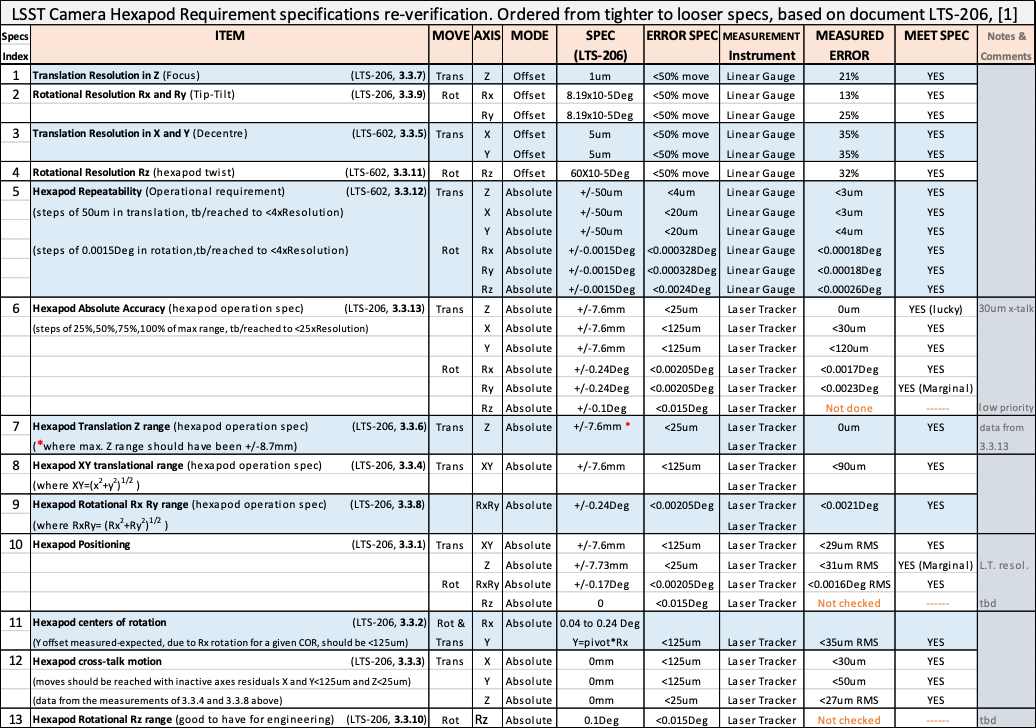
\includegraphics[width=3.125in,height=\textheight]{jira_imgs/2057.png}In
summary:\\
"Basically the fundamental requirements for Image Quality and Image
Quality correction as well as operational requirement specifications,
all seem to be met satisfactorily without load. It is not expected to
change appreciably with the camera mounted on the Hexapod and Rotator,
but some more testing, for completion, will probably be done with the
load."\\
\strut \\
\medskip
\end{minipage}
&   \\\hline
\href{https://jira.lsstcorp.org/secure/Tests.jspa#/testCase/LVV-T1599}{LVV-T1599}
&  1
& Pass &
\begin{minipage}[]{9cm}
\smallskip
This execution only tests the fixed applied since the last test case
execution. With the pass in Step 45, all test steps have passed or
passed with a slight deviation as noted in each step.\\
Therefore this execution is marked as pass.
\medskip
\end{minipage}
&   \\\hline
\href{https://jira.lsstcorp.org/secure/Tests.jspa#/testCase/LVV-T1600}{LVV-T1600}
&  2
& Initial Pass &
\begin{minipage}[]{9cm}
\smallskip

\medskip
\end{minipage}
&   \\\hline
\multicolumn{2}{r}{ T. Cycle \href{https://jira.lsstcorp.org/secure/Tests.jspa\#/testCycle/LVV-C191}{LVV-C191}:} &
\multicolumn{2}{p{10.9cm}}{\textbf{ Camera Hexapod Re-verification with ComCam }} & In Progress \\\hline
\textbf{Test Cases} &  \textbf{Ver.} & \textbf{Status} & \textbf{Comment} & \textbf{Issues} \\\toprule
\href{https://jira.lsstcorp.org/secure/Tests.jspa#/testCase/LVV-T1598}{LVV-T1598}
&  1
& Pass &
\begin{minipage}[]{9cm}
\smallskip

\medskip
\end{minipage}
&   \\\hline
\href{https://jira.lsstcorp.org/secure/Tests.jspa#/testCase/LVV-T1599}{LVV-T1599}
&  1
& Pass &
\begin{minipage}[]{9cm}
\smallskip
The ~CamHex is now on the TMA with ComCam installed.\\
For this execution only Step 26 \textbf{Test Sequence \#6 --
RawPositionSet Commands} is new and needs execution.
\medskip
\end{minipage}
&   \\\hline
\href{https://jira.lsstcorp.org/secure/Tests.jspa#/testCase/LVV-T1600}{LVV-T1600}
&  2
& Not Executed &
\begin{minipage}[]{9cm}
\smallskip

\medskip
\end{minipage}
&   \\\hline
\caption{Test Campaign Summary}
\label{table:summary}
\end{longtable}
}

\subsection{Overall Assessment}
\label{sect:overallassessment}

\hfill\break
\textbf{The following results are for the first test-cycle
\href{https://jira.lsstcorp.org/secure/Tests.jspa\#/testCycle/LVV-C114}{LVV-C114}:}\\
The camera hexapod was tested at Level 3 without a payload attached.
Depending on the test case, the hexapod was controlled through the EUI
or the CSC.\\
The overall assessment of the first test case execution was: One test
case INITIAL PASS, and two test cases: FAIL.\\
After the third execution, all three test cases belonging to test cycle
\href{https://jira.lsstcorp.org/secure/Tests.jspa\#/testCycle/LVV-C114}{LVV-C114}
of this test plan have the status: INITIAL PASS.\\
\strut \\
On the software side

\begin{itemize}
\tightlist
\item
  the EUI was reorganized to reflect the association of the commands
  with the states of the state machine correctly
  (\href{https://jira.lsstcorp.org/browse/DM-29738}{DM-29738})
\item
  the reaction of the state machine to the "clearError" command was
  improved (\href{https://jira.lsstcorp.org/browse/DM-29788}{DM-29788)}.
\item
  Some minor issues regarding rare events, such as the inappropriate
  disconnection of the encoder cable, power supplies, and network
  connection
  (\href{https://jira.lsstcorp.org/browse/DM-29791}{DM-29791},
  \href{https://jira.lsstcorp.org/browse/DM-29792}{DM-29792},
  \href{https://jira.lsstcorp.org/browse/DM-29793}{DM-29793}), have easy
  workarounds.\\
  Therefore, the corresponding test steps passed with deviations.\\
  \strut \\
\end{itemize}

The camera hexapod CSC software was improved by

\begin{itemize}
\tightlist
\item
  including checks into the camera hexapod CSC for position limits for
  the move and offset commands
  (\href{https://jira.lsstcorp.org/browse/DM-23092}{DM-23092)\\
  }
\item
  cleaning up XML for rotator and hexapods
  (\href{https://jira.lsstcorp.org/browse/DM-21699}{DM-21699})
\item
  Generating ~the inPosition event in the EFD
  (\href{https://jira.lsstcorp.org/browse/DM-29689}{DM-29689})
\item
  reporting the camera hexapod pivot point modifications in the EUI and
  the EFD (\href{https://jira.lsstcorp.org/browse/DM-29693}{DM-29693})
\item
  correcting the transition of the camera hexapod\textquotesingle s
  state machine back into standbyState
  (\href{https://jira.lsstcorp.org/browse/DM-29705}{DM-29705})
\item
  accepting the Disable command accepted and changing the state machine
  status correctly
  (\href{https://jira.lsstcorp.org/browse/DM-29706}{DM-29706})
\end{itemize}

\hfill\break
The configuration part of the CSC test case
(\href{https://jira.lsstcorp.org/secure/Tests.jspa\#/testCase/LVV-T1600}{LVV-T1600})
was not tested since the configuration system for all CSC is still under
development. The hexapod acceleration and velocity changes are not done
by stand-alone commands anymore and were, therefore, not tested. Since
the state machine of the CSC is still under development and will change
to a standbyState-entry state machine, the state machine transitions
were only partially tested as needed to conduct the other tests.\\
\strut \\
At the beginning of this verification activity, the hardware of the
camera hexapod presented issues in actuators 3 and 6. Both had dead
encoder zones that made the hexapod stop immediately. Recovery needed
direct intervention at the issue-causing actuator. The problem was
solved by taking out \textbf{all} actuators and servicing them by
cleaning the encoder band from Teflon and grease/oil and reassembling
the hexapod. In addition, during the service, the cables to the encoders
were found to be damaged due to the movements of the actuators. This
triggered a redesign of the actuator heads that is currently ongoing.
(see \href{https://jira.lsstcorp.org/browse/FRACAS-28}{FRACAS-28~}for
the actuator 3 failure and
\href{https://jira.lsstcorp.org/browse/FRACAS-54}{FRACAS-54~}for the
actuator 6 failure).\\
\strut \\
Though not directly part of this verification testing, a random failure
(a feedback fault in Drive 0 and Drive 2) caused significant delays
during test execution. The encoders inside of the actuators as well as
the drives themselves, were first suspected as the cause for the
failure. The actuators could be excluded as the origin of the fault by
exchanging the cabling between the actuators. The drives did not present
any obvious failure reason. The issue was solved after finishing this
test by exchanging the cables to one actuator and testing that this
solution could be reproduced by changing the cable from between the
drives. All cables were exchanged. The problem did not appear again.\\
\strut \\
Apart from the aforementioned issues, the camera hexapod did not reach
the XYZ accuracy as required
(\href{https://jira.lsstcorp.org/browse/LVV-19501}{LVV-19501)~}at the
beginning of the testing campaign.\\
This hardware-related issue concerns the following requirements

\begin{itemize}
\tightlist
\item
  \href{https://jira.lsstcorp.org/browse/LVV-18622}{LTS-206-REQ-0164-V-02:
  3.5.12\_1 Positioning - LSST Re-verification}
  \href{https://jira.lsstcorp.org/browse/LVV-18631}{}
\item
  \href{https://jira.lsstcorp.org/browse/LVV-18631}{LTS-206-REQ-0178-V-02:
  3.5.24\_1 Hexapod Absolute Accuracy - LSST Re-verification}.\\
  \strut \\
\end{itemize}

Specifically, the tests on the positioning in X, Y, and Z translation
combined with rotation failed to reach the required precision. The same
issue was observed for the hexapod\textquotesingle s absolute accuracy.
The reasons were lying, most likely in the measurement setup itself. The
laser tracker measurements are at the limit of the laser
tracker\textquotesingle s precision, and the MITUTOYO gauges mounts were
a preliminary solution. Testing the camera hexapod with an improved
MITUTOYO setup has shown that the same requirements are fulfilled for
the camera hexapod.\\
\strut \\
All executed hardware tests passed, as mentioned at the beginning of
this summary. Some measurements for the range in Z direction and
rotation around the Z-axis were given little priority since they are
testing a movement that is not expected to be used during normal
operations and were not performed due to missing time reasons.\\
\strut \\
\textbf{The following results are for the second
test-cycle~}\href{https://jira.lsstcorp.org/secure/Tests.jspa\#/testCycle/LVV-C191}{LVV-C191}:\\

\begin{itemize}
\tightlist
\item
  The main difference for this test cycle consists of ComCam being
  attached to the rotator.
\item
  All executed hardware tests passed again. Some measurements for the
  rotation around the Z-axis were given little priority since they are
  testing a movement that is not expected to be used during normal
  operations and were not performed due to missing time reasons.
\item
  The test case for the Camera Hexapod \textbf{Hardware
  Functional~}Re-verification
  (\href{https://jira.lsstcorp.org/secure/Tests.jspa\#/testCase/LVV-T1598}{LVV-T1598
  (1.0)}) has passed.
\item
  The
  \href{https://jira.lsstcorp.org/secure/Tests.jspa\#/testCase/LVV-T1599}{LVV-T1599}
  Camera Hexapod \textbf{Software Functional~}Re-verification test case
  was most successfully executed in the previous test cycle. Only one
  command was missing to be tested for the EUI. This test was
  successfully completed. Several requirements considering the telemetry
  and the Lookup Tables (LUTs) need to be tested together with the CSC
  (compensation mode) and were moved to the SAL test case LVV-T1600.
\end{itemize}

\subsection{Recommended Improvements}
\label{sect:recommendations}

\textbf{The following recommendations are for the situation after the
first test-cycle
\href{https://jira.lsstcorp.org/secure/Tests.jspa\#/testCycle/LVV-C114}{LVV-C114}:}\\
To improve the situation before the next test cycle, it is recommended
to finish the development of the camera hexapod low-level controller,
the EUI, and the CSC.\\
The EUI and CSC software tests regarding the state machine should be
executed when the state machine is updated to the standbyState-entry
state machine. Beforehand, the test cases should be updated to account
for state machine tests.\\
The configuration part of the CSC test case
(\href{https://jira.lsstcorp.org/secure/Tests.jspa\#/testCase/LVV-T1600}{LVV-T1600})
should be updated to account for the change in accordance with \citeds{LSE-209}
and need to be tested for the first time.\\
The camera hexapod acceleration and velocity changes should now be
tested as part of the configuration tests.\\
\strut \\
For the hardware, the camera hexapod should always be tested starting
from the origin to avoid possible hysteresis.\\
Each test step to measure the absolute accuracy of the camera hexapod
should be repeated at least three times to ensure the accuracy of the
test results.\\
\strut \\
The following hardware tests from the MOOG testing sequence should be
included

\begin{itemize}
\tightlist
\item
  3.3.10 Hexapod Rotational Rz range
\item
  3.3.1 ~Only the hexapod positioning in Rz. The rest was tested and is
  within specification.
\item
  3.3.13 Measure Rz
\end{itemize}

\hfill\break
\textbf{The following recommendations are for the situation after the
second test-cycle
\href{https://jira.lsstcorp.org/secure/Tests.jspa\#/testCycle/LVV-C191}{LVV-C191}:}\\
\strut \\
The hardware-related tests need to be re-executed when the redesign and
reconstruction of the actuator are finished.\\
This involves new hardware and is, therefore, not part of this test plan
for the re-verification of the vendor-delivered hardware.\\
\strut \\
During the test with the new hardware, including a test over the full
range up to the software limits. It must include the +/- 8.7mm position.

\newpage
\section{Detailed Test Results}
\label{sect:detailedtestresults}

\subsection{Test Cycle LVV-C114 }

Open test cycle {\it \href{https://jira.lsstcorp.org/secure/Tests.jspa#/testrun/LVV-C114}{Camera Hexapod Re-Verification}} in Jira.

Test Cycle name: Camera Hexapod Re-Verification\\
Status: Done

Re-verify the hardware and software requirements for the camera rotator
that MOOG previously tested.

\subsubsection{Software Version/Baseline}
\begin{enumerate}
\tightlist
\item
  Camera Hexapod Control Software with at least SAL v4.0
\item
  EFD with at least SAL v4.0
\end{enumerate}

\subsubsection{Configuration}
The configuration for the first test cycle is as follows:

\begin{itemize}
\tightlist
\item
  the hexapod is without a representative camera load
\item
  using the offlineState-entry state machine.
\end{itemize}

\subsubsection{Test Cases in LVV-C114 Test Cycle}

\paragraph{ LVV-T1598 - Camera Hexapod Hardware Functional Re-Verification }\mbox{}\\

Version \textbf{1}.
Status \textbf{Approved}.
Open  \href{https://jira.lsstcorp.org/secure/Tests.jspa#/testCase/LVV-T1598}{\textit{ LVV-T1598 } }
test case in Jira.

The objective of this test case is to re-verify the functional
requirements of the camera hexapod\textquotesingle s hardware after
shipment from the vendor\textquotesingle s facility to the Summit, as
defined in \citeds{LTS-206}.\\
This test case will only exercise the functionality that was executed
previously and meets the following criteria:

\begin{itemize}
\tightlist
\item
  It only requires the camera hexapod to be operable
\item
  Only requires the vendor\textquotesingle s EUI software and hardware
  via local control
\item
  Requires a laser tracker, mechanical gauges, induction current probe,
  temperature sensors
\item
  This test case can be executed with or without the camera rotator to
  be loaded with the camera simulated mass or actual camera hardware.\\
  \strut \\
\end{itemize}

The hardware functional requirements were previously verified during the
test campaign by the vendor at the vendor\textquotesingle s facility and
accepted by LSST during the Factory Acceptance Test review.\\
The test procedure used during the vendor\textquotesingle s acceptance
testing is the \emph{LSST Hexapods-Rotator Acceptance Test Procedure}
which is attached to this test case.\\
The test steps of this test case reference the vendor\textquotesingle s
acceptance test procedure for the details on how to perform the test.\\
The reference to the vendor\textquotesingle s acceptance test procedure
is included to perform the test similarly as it was performed
previously.\\
There are also deviations to the vendor\textquotesingle s acceptance
test procedure included in the test cases.\\
This became necessary due to the differences in the verification
configuration and deviations to requirements granted to the vendor by
Rubin.\\
\strut \\
See the attached \emph{LSST Rotator Hexapod\textquotesingle s Manual}
for more information on how to operate the hexapod.

\textbf{ Preconditions}:\\
Prior to the execution of this test case to re-verify the Camera Hexapod
hardware functional requirements, the following Summit tasks must be
completed:

\begin{itemize}
\tightlist
\item
  The Hexapod has been installed on the camera cart

  \begin{itemize}
  \tightlist
  \item
    \url{https://jira.lsstcorp.org/browse/SUMMIT-3224}
  \end{itemize}
\item
  The Hexapod Controller has been deployed on the summit

  \begin{itemize}
  \tightlist
  \item
    \url{https://jira.lsstcorp.org/browse/SUMMIT-3229}
  \end{itemize}
\item
  Boxes for the Hexapod have been transported to the 3rd level

  \begin{itemize}
  \tightlist
  \item
    \url{https://jira.lsstcorp.org/browse/SUMMIT-3230}
  \end{itemize}
\item
  All Hexapod cables and cabinets have been prepared for integration
  with the camera cart

  \begin{itemize}
  \tightlist
  \item
    \url{https://jira.lsstcorp.org/browse/SUMMIT-3231}
  \end{itemize}
\item
  The offset has been installed onto the integrating structure

  \begin{itemize}
  \tightlist
  \item
    \url{https://jira.lsstcorp.org/browse/SUMMIT-3293}
  \end{itemize}
\item
  The Camera Hexapod electrical connections have been tested

  \begin{itemize}
  \tightlist
  \item
    \url{https://jira.lsstcorp.org/browse/SUMMIT-3294}
  \end{itemize}
\end{itemize}

Execution status: {\bf Initial Pass }

Final comment:\\During the execution, the hexapod presents various random faults. The
problem was solved by exchanging the cabling for all actuators.
See\href{https://jira.lsstcorp.org/browse/FRACAS-64}{~FRACAS-64} and
\href{https://jira.lsstcorp.org/browse/FRACAS-56}{FRACAS-56}.\\
Please find the details of these tests in the attached report. This is
the summary from the report:\\
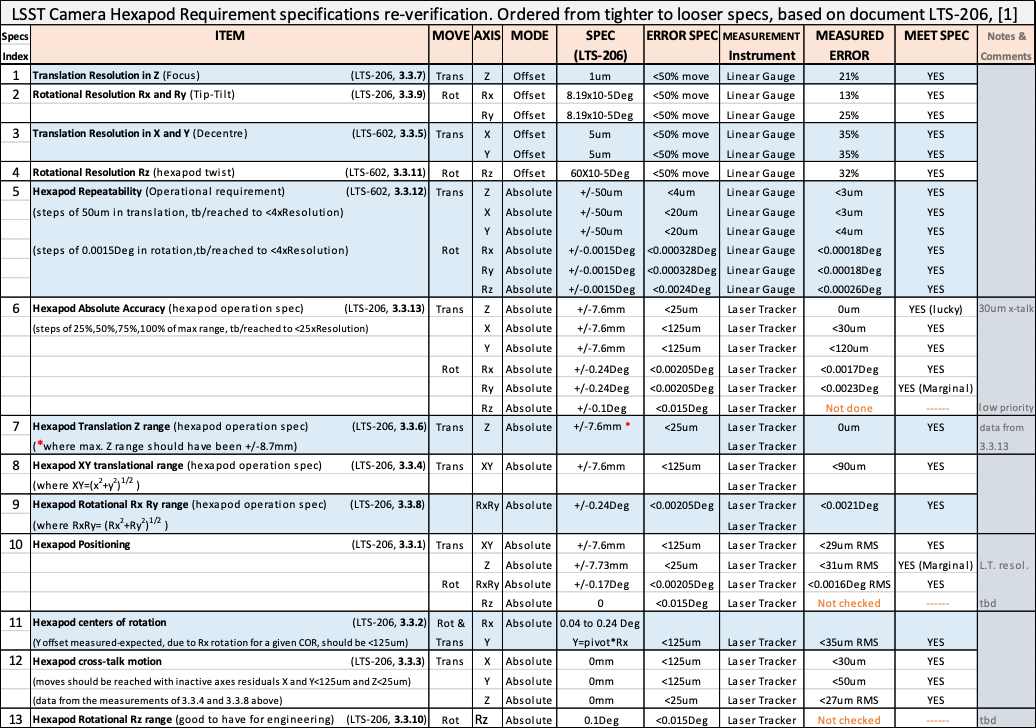
\includegraphics[width=3.125in,height=\textheight]{jira_imgs/2057.png}In
summary:\\
"Basically the fundamental requirements for Image Quality and Image
Quality correction as well as operational requirement specifications,
all seem to be met satisfactorily without load. It is not expected to
change appreciably with the camera mounted on the Hexapod and Rotator,
but some more testing, for completion, will probably be done with the
load."\\
\strut \\


Detailed steps results:

\begin{tabular}{p{2cm}p{14cm}}
\toprule
Step 1 & Step Execution Status: \textbf{ Not Executed } \\ \hline
\end{tabular}
 Description \\
{\footnotesize
\textbf{STARTING THE EUI}\\
\strut \\
Connect to the hexapod management computer using X2Go\\
Open a terminal\\
change to the folder\\
\strut \\
cd /rubin/hexapod/build/\\
\strut \\
Start the EUI with the command:\\
\strut \\
./runCamHexEui\\
\strut \\
for the camera and the M2 hexapod, respectively.

}
\hdashrule[0.5ex]{\textwidth}{1pt}{3mm}
  Expected Result \\
{\footnotesize
The EUI is in the Offline State/PublishOnly substate and is able to
publish through SAL but cannot receive commands.

}
\hdashrule[0.5ex]{\textwidth}{1pt}{3mm}
  Actual Result \\
{\footnotesize

}
\begin{tabular}{p{2cm}p{14cm}}
\toprule
Step 2 & Step Execution Status: \textbf{ Not Executed } \\ \hline
\end{tabular}
 Description \\
{\footnotesize
\textbf{OFFLINESTATE/AVAILABLESTATE}\\
On the Main tab, select the "Offline SubState Command" field in the
Commands to Send section, set the Offline SubState Triggers to "System
Ready" and click on the Send Command button.\\
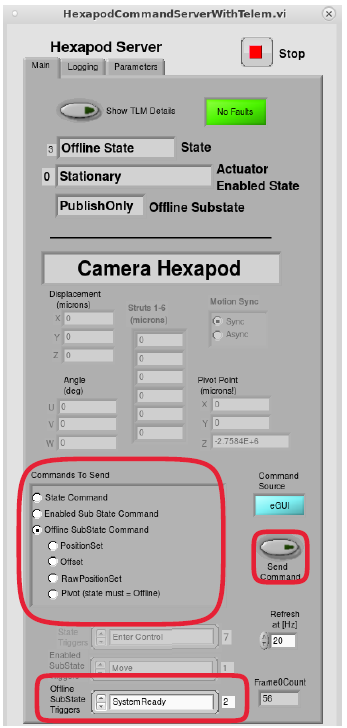
\includegraphics[width=1.79167in,height=\textheight]{jira_imgs/1024.png}

}
\hdashrule[0.5ex]{\textwidth}{1pt}{3mm}
  Expected Result \\
{\footnotesize
The system transitions from the OfflineState/PublishOnly substate to the
OfflineState/AvailableState substate and the Command Source says eGUI.\\
\strut \\

}
\hdashrule[0.5ex]{\textwidth}{1pt}{3mm}
  Actual Result \\
{\footnotesize

}
\begin{tabular}{p{2cm}p{14cm}}
\toprule
Step 3 & Step Execution Status: \textbf{ Not Executed } \\ \hline
\end{tabular}
 Description \\
{\footnotesize
\textbf{OFFLINESTATE -\textgreater{} STANDBYSTATE}\\
Click on the State Command field in the Commands to Send section.\\
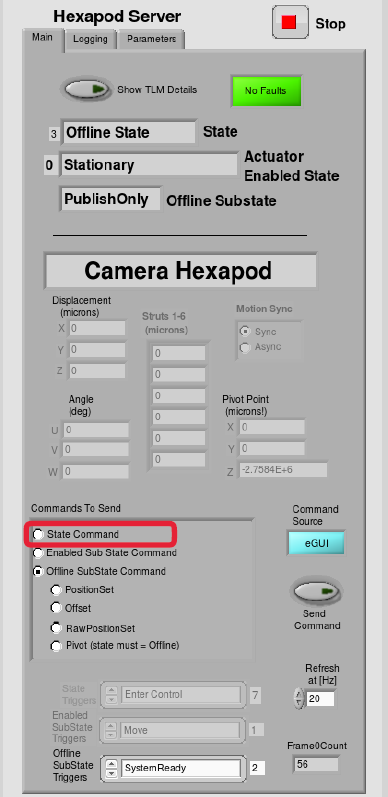
\includegraphics[width=1.79167in,height=\textheight]{jira_imgs/1028.png}

}
\hdashrule[0.5ex]{\textwidth}{1pt}{3mm}
  Expected Result \\
{\footnotesize
The State Triggers dialogue box shown below becomes visible.\\
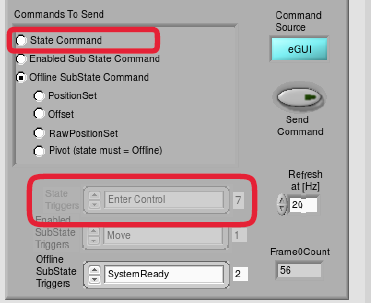
\includegraphics[width=1.79167in,height=\textheight]{jira_imgs/1029.png}

}
\hdashrule[0.5ex]{\textwidth}{1pt}{3mm}
  Actual Result \\
{\footnotesize

}
\begin{tabular}{p{2cm}p{14cm}}
\toprule
Step 4 & Step Execution Status: \textbf{ Not Executed } \\ \hline
\end{tabular}
 Description \\
{\footnotesize
Scroll through the available trigger options to select "Enter Control"
and click the Send Command button.

}
\hdashrule[0.5ex]{\textwidth}{1pt}{3mm}
  Expected Result \\
{\footnotesize
The system transitions to the Standby state and the primary state
display box at the top of the Main says Standby state.

}
\hdashrule[0.5ex]{\textwidth}{1pt}{3mm}
  Actual Result \\
{\footnotesize

}
\begin{tabular}{p{2cm}p{14cm}}
\toprule
Step 5 & Step Execution Status: \textbf{ Not Executed } \\ \hline
\end{tabular}
 Description \\
{\footnotesize
\textbf{STANDBYSTATE -\textgreater{} DISABLEDSTATE}\\
From the StandbyState, send a Start State command.

}
\hdashrule[0.5ex]{\textwidth}{1pt}{3mm}
  Expected Result \\
{\footnotesize
The system transitions into DisabledState and the current configuration
parameters are maintained from the default parameters or from the
previous DDS start command.~

}
\hdashrule[0.5ex]{\textwidth}{1pt}{3mm}
  Actual Result \\
{\footnotesize

}
\begin{tabular}{p{2cm}p{14cm}}
\toprule
Step 6 & Step Execution Status: \textbf{ Not Executed } \\ \hline
\end{tabular}
 Description \\
{\footnotesize
\textbf{DISABLEDSTATE -\textgreater{} ENABLEDSTATE}\\
From the DisabledState, send an Enable State Command.~

}
\hdashrule[0.5ex]{\textwidth}{1pt}{3mm}
  Expected Result \\
{\footnotesize
The system transitions into the EnabledState/Stationary substate, the
motor drives are enabled and and motion can be commanded.~

}
\hdashrule[0.5ex]{\textwidth}{1pt}{3mm}
  Actual Result \\
{\footnotesize

}
\begin{tabular}{p{2cm}p{14cm}}
\toprule
Step 7 & Step Execution Status: \textbf{ Not Executed } \\ \hline
\end{tabular}
 Description \\
{\footnotesize
\textless conditional state\textgreater{}\\
\textbf{FAULTSTATE}\\
If a Fault occurs in any of the other states, the system will
automatically transition to the Fault State. While in the Fault state,
send a clearError.\\
\ul{Note:} If the fault that occurs goes through the interlock system,
reset the safety relay switch and send a clearError command.

}
\hdashrule[0.5ex]{\textwidth}{1pt}{3mm}
  Expected Result \\
{\footnotesize
The system transitions back to the OfflineState/PublishOnly substate.
(Go back to Step 3)

}
\hdashrule[0.5ex]{\textwidth}{1pt}{3mm}
  Actual Result \\
{\footnotesize

}
\begin{tabular}{p{2cm}p{14cm}}
\toprule
Step 8 & Step Execution Status: \textbf{ Initial Pass } \\ \hline
\end{tabular}
 Description \\
{\footnotesize
\textbf{Follow \emph{3.3.1 Positioning} of the LSST Hexapods-Rotator
Acceptance Test Procedure, Sheet 23-24.}

}
\hdashrule[0.5ex]{\textwidth}{1pt}{3mm}
  Test Data \\
 {\footnotesize
\textbf{Deviation:~}Test this with no performance payload and at a
single elevation angle of zero degrees. Wait for 39s between movements.

}
\hdashrule[0.5ex]{\textwidth}{1pt}{3mm}
  Expected Result \\
{\footnotesize
The position of the hexapod is able to be commanded and no software
limits or limit switches are tripped.\\
The position of the hexapod is able to reach the commanded positions
within the absolute accuracy specifications of 25um in Z, 125um in XY,
205x10-5deg in RXRY, and 1500x10-5deg in RZ.

}
\hdashrule[0.5ex]{\textwidth}{1pt}{3mm}
  Actual Result \\
{\footnotesize
The camera hexapod was measured with the laser tracker during the 32
movements.\\
From the attached report:\\
"The camera hexapod positioning mostly meets requirements. Except for
some marginal outliers, the XY accuracy is 29um RMS and the RxRy angular
accuracy is 0.0015Deg RMS both meeting specs. The Z positioning is 31um
RMS, apparently not meeting the spec of 25um, but this is because the
laser tracker resolution is roughly 30um (in fact, most likely all
laser-tracker-based measurements are limited by this resolution value).
The Rz requirement of positioning accuracy \textless0.015Deg has not
been checked (tbd)."

}
\begin{tabular}{p{2cm}p{14cm}}
\toprule
Step 9 & Step Execution Status: \textbf{ Initial Pass } \\ \hline
\end{tabular}
 Description \\
{\footnotesize
\textbf{Follow \emph{3.3.2 Centers of Rotation} of the LSST
Hexapods-Rotator Acceptance Test Procedure, Sheet 24-25.}

}
\hdashrule[0.5ex]{\textwidth}{1pt}{3mm}
  Test Data \\
 {\footnotesize
\textbf{Deviation:~}Record pivot position through the EUI. Wait for 39s
between movements.

}
\hdashrule[0.5ex]{\textwidth}{1pt}{3mm}
  Expected Result \\
{\footnotesize
The center of rotation is able to be moved.

}
\hdashrule[0.5ex]{\textwidth}{1pt}{3mm}
  Actual Result \\
{\footnotesize
From the attached report:\\
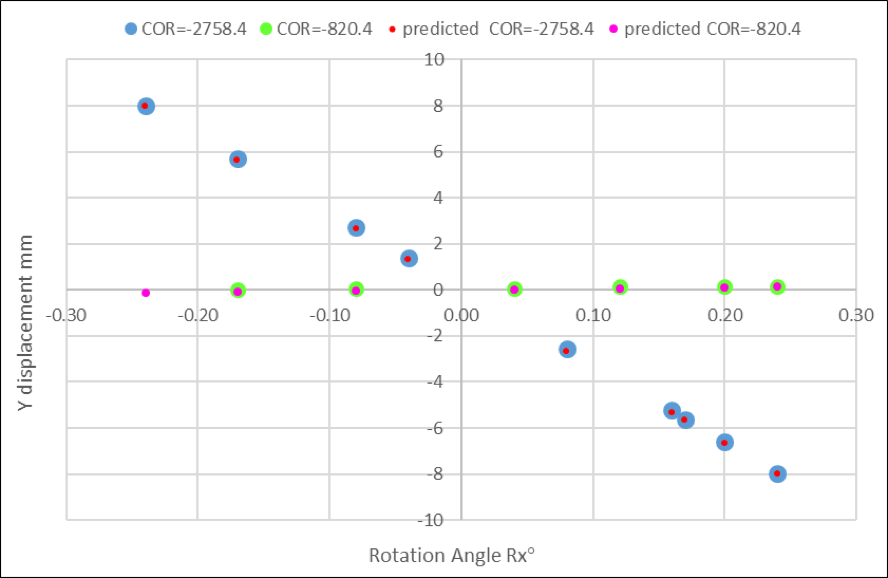
\includegraphics[width=4.46875in,height=\textheight]{jira_imgs/2055.png}"The
measured and predicted Y displacement for a commanded Rx rotation
coincide to better than 35um. The data on COR -820400um (-820.4 on the
plot) corresponding to pivot on rotator surface, is from March 2021. The
data for COR -2758400um (-2758.4 on the plot) pivot at L1S1, is from
March 2021 and June 2021 after the camera hexapod actuators
refurbishing, both sets of data coincide well. So COR definition works
as expected."

}
\begin{tabular}{p{2cm}p{14cm}}
\toprule
Step 10 & Step Execution Status: \textbf{ Pass } \\ \hline
\end{tabular}
 Description \\
{\footnotesize
\textbf{Follow \emph{3.3.3 Cross-Talk Motion~}of the LSST
Hexapods-Rotator Acceptance Test Procedure, Sheet 25.}

}
\hdashrule[0.5ex]{\textwidth}{1pt}{3mm}
  Expected Result \\
{\footnotesize
There is no cross-talk observed (actuator positioning errors and
erroneous geometry are minimal).

}
\hdashrule[0.5ex]{\textwidth}{1pt}{3mm}
  Actual Result \\
{\footnotesize
From the attached report: "(a) Using the data from the X and Y
Translational Range measurements (LTS-206, 3.3.4) and (b) from Rx and Ry
Rotational range measurements (LTS-206, 3.3.8), the camera hexapod
translation range's cross talk is shown to meet specs. All commanded
moves reach the destination with the inactive dimensions' residuals
being \textless125um for X and Y and \textless25um for Z."

}
\begin{tabular}{p{2cm}p{14cm}}
\toprule
Step 11 & Step Execution Status: \textbf{ Pass } \\ \hline
\end{tabular}
 Description \\
{\footnotesize
\textbf{Follow \emph{3.3.4 Radial (X and Y) Translational Range~}of the
LSST Hexapods-Rotator Acceptance Test Procedure, Sheet 25.}

}
\hdashrule[0.5ex]{\textwidth}{1pt}{3mm}
  Test Data \\
 {\footnotesize
\textbf{Deviation:~}Only test at a zero degree elevation angle. Wait for
39s between movements.

}
\hdashrule[0.5ex]{\textwidth}{1pt}{3mm}
  Expected Result \\
{\footnotesize
The hexapod is capable of moving to the positions in the XY plane listed
in the Acceptance Test Procedure.

}
\hdashrule[0.5ex]{\textwidth}{1pt}{3mm}
  Actual Result \\
{\footnotesize
From the attached report: The camera hexapod translation range meets
specs. All commanded values range within 125um. ~ ~ ~ ~ ~

}
\begin{tabular}{p{2cm}p{14cm}}
\toprule
Step 12 & Step Execution Status: \textbf{ Initial Pass } \\ \hline
\end{tabular}
 Description \\
{\footnotesize
\textbf{Follow \emph{3.3.6 Axial (Z) Translation Range~}of the LSST
Hexapods-Rotator Acceptance Test Procedure, Sheet 27.}

}
\hdashrule[0.5ex]{\textwidth}{1pt}{3mm}
  Test Data \\
 {\footnotesize
\textbf{Deviation:~}Only test at a zero degree elevation angle. Wait for
39s between movements.

}
\hdashrule[0.5ex]{\textwidth}{1pt}{3mm}
  Expected Result \\
{\footnotesize
The hexapod is capable of moving to the positions in the Z plane listed
in the Acceptance Test Procedure.~

}
\hdashrule[0.5ex]{\textwidth}{1pt}{3mm}
  Actual Result \\
{\footnotesize
From the attached report: "The camera hexapod Z translational range
meets specs. Positions reached within 25um. This test was not done
exactly as the Moog procedure says (+/-8.7mm) because of time
constraints. Instead, we just extracted the data from the absolute
accuracy test."

}
\begin{tabular}{p{2cm}p{14cm}}
\toprule
Step 13 & Step Execution Status: \textbf{ Pass } \\ \hline
\end{tabular}
 Description \\
{\footnotesize
\textbf{Follow \emph{3.3.8 Rotational Range Around X-Axis (Tip) and
Y-Axis (Tilt)~}of the LSST Hexapods-Rotator Acceptance Test Procedure,
Sheet 28-29.}

}
\hdashrule[0.5ex]{\textwidth}{1pt}{3mm}
  Test Data \\
 {\footnotesize
\textbf{Deviation:~}Only test at a zero degree elevation angle. Wait for
39s between movements.

}
\hdashrule[0.5ex]{\textwidth}{1pt}{3mm}
  Expected Result \\
{\footnotesize
The hexapod is capable of moving to the positions in the RXRY plane
listed in the Acceptance Test Procedure.

}
\hdashrule[0.5ex]{\textwidth}{1pt}{3mm}
  Actual Result \\
{\footnotesize
From the attached report: "The camera hexapod rotational range meets
specs. Positions reached within 0.0021Deg."

}
\begin{tabular}{p{2cm}p{14cm}}
\toprule
Step 14 & Step Execution Status: \textbf{ Not Executed } \\ \hline
\end{tabular}
 Description \\
{\footnotesize
\textbf{Follow \emph{3.3.10 Rotation Range Around Z-Axis (Twist)~}of the
LSST Hexapods-Rotator Acceptance Test Procedure, Sheet 30.}

}
\hdashrule[0.5ex]{\textwidth}{1pt}{3mm}
  Test Data \\
 {\footnotesize
\textbf{Deviation:~}Only test at a zero degree elevation angle. Wait for
39s between movements.

}
\hdashrule[0.5ex]{\textwidth}{1pt}{3mm}
  Expected Result \\
{\footnotesize
The hexapod is capable of moving to the positions in the RZ-axis listed
in the Acceptance Test Procedure.

}
\hdashrule[0.5ex]{\textwidth}{1pt}{3mm}
  Actual Result \\
{\footnotesize
From the attached report: "Never checked the full range because of time
and not critical, so lower priority, TBD anyway."

}
\begin{tabular}{p{2cm}p{14cm}}
\toprule
Step 15 & Step Execution Status: \textbf{ Initial Pass } \\ \hline
\end{tabular}
 Description \\
{\footnotesize
\textbf{Follow \emph{3.3.12 Hexapod Repeatability} of the LSST
Hexapods-Rotato Acceptance Test Procedure, Sheet 31.}

}
\hdashrule[0.5ex]{\textwidth}{1pt}{3mm}
  Expected Result \\
{\footnotesize
The repeatability is as good as the test equipment can capture. This
means that the repeatability is limited by the resolution of the test
equipment.

}
\hdashrule[0.5ex]{\textwidth}{1pt}{3mm}
  Actual Result \\
{\footnotesize
From the attached report:\\
\textbf{"Table 5}. Shows that translation repeatability tests meet
specifications, {[}1{]} and {[}4{]}. Starting from hexapod position
(0,0,0,0,0,0), repeatability testing moves of 50um in absolute mode, are
executed to within the specs of \textless4um for Z moves and
\textless20um for X and Y moves. Note that starting from any other
hexapod position away from the zero, means a different setup for the
Linear Gauges, so it is not practical to do, because of time."

}
\begin{tabular}{p{2cm}p{14cm}}
\toprule
Step 16 & Step Execution Status: \textbf{ Initial Pass } \\ \hline
\end{tabular}
 Description \\
{\footnotesize
\textbf{Follow \emph{3.3.13 Hexapod Absolute Accuracy~}of the LSST
Hexapods-Rotator Acceptance Test Procedure, Sheet 38-42.}

}
\hdashrule[0.5ex]{\textwidth}{1pt}{3mm}
  Test Data \\
 {\footnotesize
\textbf{Deviation:~}Only test at a zero degree elevation angle. Wait for
39s between movements.

}
\hdashrule[0.5ex]{\textwidth}{1pt}{3mm}
  Expected Result \\
{\footnotesize
The accuracy of the hexapod is good enough to be consistently repeated.
The accuracy of the hexapod is at least the following: 25um in Z, 125um
in XY, 205x10-5deg in RXRY, and 1500x10-5deg in RZ.

}
\hdashrule[0.5ex]{\textwidth}{1pt}{3mm}
  Actual Result \\
{\footnotesize
Data for (b) assembled from positioning and maximum range data.\\
Hexapod Absolute Accuracy in Rz not measured.\\
\strut \\
From the attached report: "a) shows that the camera hexapod translation
Absolute Accuracy meets specs. All commanded moves in X, Y or Z, are
reached within the required specs of \textless25um for Z and
\textless125um for X and Y. (b) shows that the Camera Hexapod Absolute
Rotation Accuracy meets the specs. Commanded moves are reached within
the required specs of 0.0021Deg for Rx, Ry, {[}4{]}. Unfortunately, a
set of measurements of Rz, as defined in {[}2{]}, is missing. Left
behind because it isn't a movement expected to be used in operation, so
was given little priority."

}
\begin{tabular}{p{2cm}p{14cm}}
\toprule
Step 17 & Step Execution Status: \textbf{ Initial Pass } \\ \hline
\end{tabular}
 Description \\
{\footnotesize
\textbf{Follow \emph{3.3.16 Hexapod Radial (X and Y) and Axial (Z)
Velocity Range} and~\emph{3.3.17 Hexapod Rotational Velocity~}of the
LSST Hexapods-Rotator Acceptance Test Procedure, Sheet 43-44.}

}
\hdashrule[0.5ex]{\textwidth}{1pt}{3mm}
  Test Data \\
 {\footnotesize
\textbf{Deviation:~}Only test this using synchronous mode. Wait for 39s
between movements.

}
\hdashrule[0.5ex]{\textwidth}{1pt}{3mm}
  Expected Result \\
{\footnotesize
The hexapod velocity exceeds the 152um/s in XY and 0.0039deg/s in RXYRY
and RZ requirements.

}
\hdashrule[0.5ex]{\textwidth}{1pt}{3mm}
  Actual Result \\
{\footnotesize
Though this point was not investigated separately the camera hexapod
reached all positions in a timely manner with all actuators nearly at
the same time.\\
Small movements as used for science operations take only a few seconds
what is well with the time frame given to the hexapod to reach its
position between two exposures of the camera.

}
\begin{tabular}{p{2cm}p{14cm}}
\toprule
Step 18 & Step Execution Status: \textbf{ Pass } \\ \hline
\end{tabular}
 Description \\
{\footnotesize
\textbf{Follow \emph{3.3.18 Hexapod Heat Dissipation~}of the LSST
Hexapods-Rotator Acceptance Test Procedure, Sheet 44.}

}
\hdashrule[0.5ex]{\textwidth}{1pt}{3mm}
  Expected Result \\
{\footnotesize
The current measured by the inductive current probes is calculated to
meet the heat dissipation requirement.

}
\hdashrule[0.5ex]{\textwidth}{1pt}{3mm}
  Actual Result \\
{\footnotesize
The heat dissipation was monitored through the temperature sensors at
the actuators and all temperatures stayed with in the allowed limits
during the test.

}

\paragraph{ LVV-T1599 - Camera Hexapod Software Functional Re-verification }\mbox{}\\

Version \textbf{1}.
Status \textbf{Approved}.
Open  \href{https://jira.lsstcorp.org/secure/Tests.jspa#/testCase/LVV-T1599}{\textit{ LVV-T1599 } }
test case in Jira.

The objective of this test case is to re-verify the functional
requirements of the camera hexapod\textquotesingle s software after the
shipment of the hardware from the vendor\textquotesingle s facility to
the Summit, as defined in \citeds{LTS-206} and \citeds{LTS-160}.\\
This test case will only exercise the functionality that was executed
previously and meets the following criteria:

\begin{itemize}
\tightlist
\item
  It only requires the camera hexapod to be operable
\item
  It only requires testing of the synchronous mode

  \begin{itemize}
  \tightlist
  \item
    \textbf{Asynchronous mode is not a standard mode of operation}
  \end{itemize}
\item
  Only requires the vendor\textquotesingle s EUI software and hardware
  via local control

  \begin{itemize}
  \tightlist
  \item
    It does \textbf{NOT} require integration with SAL
  \end{itemize}
\item
  This test case can be executed with or without the camera rotator to
  be loaded with the camera simulated mass or actual camera hardware.
\end{itemize}

The software functional requirements were previously verified during the
test campaign by the vendor at the vendor\textquotesingle s facility and
accepted by LSST during the Factory Acceptance Test review.\\
The test procedure used during the vendor\textquotesingle s acceptance
testing is the \emph{LSST Hexapods-Rotator Software Acceptance Test
Procedure} which is attached to this test case.\\
The test steps of this test case are taken directly from that document
in order to perform the test in a similar way as was performed
previously. The test steps include changes noted by the vendor.\\
\strut \\
See the attached \emph{LSST Hexapod Operator\textquotesingle s Manual}
for more information on how to operate the hexapod.

\textbf{ Preconditions}:\\
Prior to the execution of this test case to re-verify the Camera Hexapod
hardware functional requirements, the following Summit tasks must be
completed:

\begin{itemize}
\tightlist
\item
  The Hexapod has been installed on the camera cart

  \begin{itemize}
  \tightlist
  \item
    \url{https://jira.lsstcorp.org/browse/SUMMIT-3224}
  \end{itemize}
\item
  The Hexapod Controller has been deployed on the summit

  \begin{itemize}
  \tightlist
  \item
    \url{https://jira.lsstcorp.org/browse/SUMMIT-3229}
  \end{itemize}
\item
  Boxes for the Hexapod have been transported to the 3rd level

  \begin{itemize}
  \tightlist
  \item
    \url{https://jira.lsstcorp.org/browse/SUMMIT-3230}
  \end{itemize}
\item
  All Hexapod cables and cabinets have been prepared for integration
  with the camera cart

  \begin{itemize}
  \tightlist
  \item
    \url{https://jira.lsstcorp.org/browse/SUMMIT-3231}
  \end{itemize}
\item
  The offset has been installed onto the integrating structure

  \begin{itemize}
  \tightlist
  \item
    \url{https://jira.lsstcorp.org/browse/SUMMIT-3293}
  \end{itemize}
\item
  The Camera Hexapod electrical connections have been tested

  \begin{itemize}
  \tightlist
  \item
    \url{https://jira.lsstcorp.org/browse/SUMMIT-3294}
  \end{itemize}
\end{itemize}

Execution status: {\bf Pass }

Final comment:\\This execution only tests the fixed applied since the last test case
execution. With the pass in Step 45, all test steps have passed or
passed with a slight deviation as noted in each step.\\
Therefore this execution is marked as pass.


Detailed steps results:

\begin{tabular}{p{2cm}p{14cm}}
\toprule
Step 1 & Step Execution Status: \textbf{ Pass } \\ \hline
\end{tabular}
 Description \\
{\footnotesize
\textbf{STARTING THE EUI}\\
\strut \\
Double click the Hexapod GUI Viewer desktop icon on the computer.

\begin{itemize}
\tightlist
\item
  This can be done on the Dell Management PC or another computer on the
  same network
\end{itemize}

}
\hdashrule[0.5ex]{\textwidth}{1pt}{3mm}
  Expected Result \\
{\footnotesize
A prompt to enter the password is shown.

}
\hdashrule[0.5ex]{\textwidth}{1pt}{3mm}
  Actual Result \\
{\footnotesize
\begin{itemize}
\tightlist
\item
  Deviation: We are using X2go now
\end{itemize}

}
\begin{tabular}{p{2cm}p{14cm}}
\toprule
Step 2 & Step Execution Status: \textbf{ Pass } \\ \hline
\end{tabular}
 Description \\
{\footnotesize
Enter the password "lsst-vnc"

\begin{itemize}
\tightlist
\item
  If the EUI isn\textquotesingle t automatically up and running when the
  VNC opens, double click on the Hexapod-eGUI icon on the VNC viewer
\end{itemize}

}
\hdashrule[0.5ex]{\textwidth}{1pt}{3mm}
  Expected Result \\
{\footnotesize
The EUI is in the Offline State/PublishOnly substate and is able to
publish through SAL but cannot receive commands.

}
\hdashrule[0.5ex]{\textwidth}{1pt}{3mm}
  Actual Result \\
{\footnotesize

}
\begin{tabular}{p{2cm}p{14cm}}
\toprule
Step 3 & Step Execution Status: \textbf{ Pass } \\ \hline
\end{tabular}
 Description \\
{\footnotesize
\textbf{OFFLINESTATE/AVAILABLESTATE}\\
On the Main tab, select the "Offline SubState Cmd" field in the Commands
to Send section, set the Offline SubState Triggers to "System Ready" and
click on the Send Command button.\\
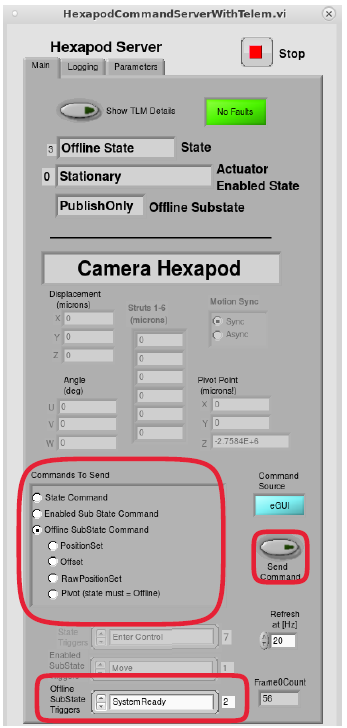
\includegraphics[width=1.79167in,height=\textheight]{jira_imgs/1024.png}

}
\hdashrule[0.5ex]{\textwidth}{1pt}{3mm}
  Expected Result \\
{\footnotesize
The system transitions from the OfflineState/PublishOnly substate to the
OfflineState/AvailableState substate and the Command Source says eGUI.\\
\strut \\

}
\hdashrule[0.5ex]{\textwidth}{1pt}{3mm}
  Actual Result \\
{\footnotesize

}
\begin{tabular}{p{2cm}p{14cm}}
\toprule
Step 4 & Step Execution Status: \textbf{ Pass } \\ \hline
\end{tabular}
 Description \\
{\footnotesize
\textbf{OFFLINESTATE -\textgreater{} STANDBYSTATE}\\
Click on the State Command field in the Commands to Send section.\\
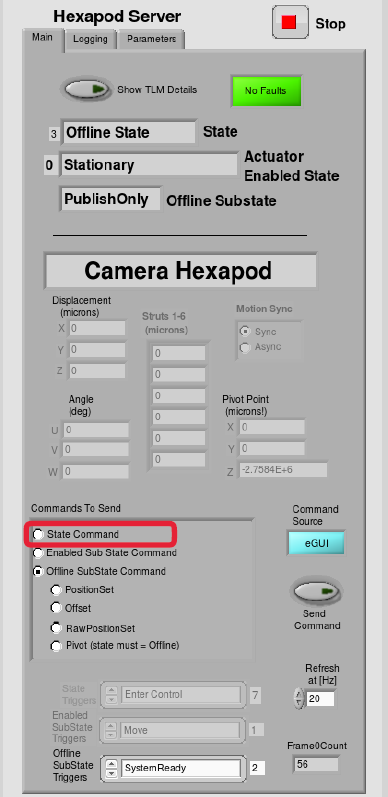
\includegraphics[width=1.79167in,height=\textheight]{jira_imgs/1028.png}

}
\hdashrule[0.5ex]{\textwidth}{1pt}{3mm}
  Expected Result \\
{\footnotesize
The State Triggers dialogue box shown below becomes visible.\\
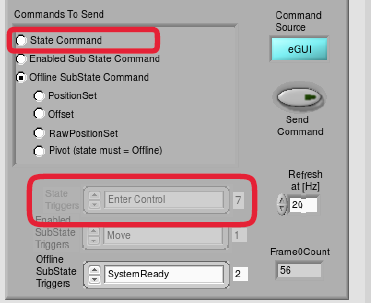
\includegraphics[width=1.79167in,height=\textheight]{jira_imgs/1029.png}

}
\hdashrule[0.5ex]{\textwidth}{1pt}{3mm}
  Actual Result \\
{\footnotesize

}
\begin{tabular}{p{2cm}p{14cm}}
\toprule
Step 5 & Step Execution Status: \textbf{ Pass } \\ \hline
\end{tabular}
 Description \\
{\footnotesize
Scroll through the available trigger options to select "Enter Control"
and click the Send Command button.

}
\hdashrule[0.5ex]{\textwidth}{1pt}{3mm}
  Expected Result \\
{\footnotesize
The system transitions to the Standby state and the primary state
display box at the top of the Main says Standby State.

}
\hdashrule[0.5ex]{\textwidth}{1pt}{3mm}
  Actual Result \\
{\footnotesize

}
\begin{tabular}{p{2cm}p{14cm}}
\toprule
Step 6 & Step Execution Status: \textbf{ Pass } \\ \hline
\end{tabular}
 Description \\
{\footnotesize
\textbf{STANDBYSTATE -\textgreater{} DISABLEDSTATE}\\
From the StandbyState, send a Start State command.

}
\hdashrule[0.5ex]{\textwidth}{1pt}{3mm}
  Expected Result \\
{\footnotesize
The system transitions into DisabledState and the current configuration
parameters are maintained from the default parameters or from the
previous DDS start command.~

}
\hdashrule[0.5ex]{\textwidth}{1pt}{3mm}
  Actual Result \\
{\footnotesize
Yes, the configuration was correctly loaded. No invalid configuration
file was tested.

}
\begin{tabular}{p{2cm}p{14cm}}
\toprule
Step 7 & Step Execution Status: \textbf{ Pass } \\ \hline
\end{tabular}
 Description \\
{\footnotesize
\textbf{DISABLEDSTATE -\textgreater{} ENABLEDSTATE}\\
From the DisabledState, send an Enable State Command.~

}
\hdashrule[0.5ex]{\textwidth}{1pt}{3mm}
  Expected Result \\
{\footnotesize
The system transitions into the EnabledState/Stationary substate, the
motor drives are enabled and and motion can be commanded.~

}
\hdashrule[0.5ex]{\textwidth}{1pt}{3mm}
  Actual Result \\
{\footnotesize

}
\begin{tabular}{p{2cm}p{14cm}}
\toprule
Step 8 & Step Execution Status: \textbf{ Not Executed } \\ \hline
\end{tabular}
 Description \\
{\footnotesize
\textless conditional state\textgreater{}\\
\textbf{FAULTSTATE}\\
If a Fault occurs in any of the other states, the system will
automatically transition to the Fault State. While in the Fault state,
send a clearError.\\
\ul{Note:} If the fault that occurs goes through the interlock system,
reset the safety relay switch and send a clearError command.

}
\hdashrule[0.5ex]{\textwidth}{1pt}{3mm}
  Expected Result \\
{\footnotesize
The system transitions back to the OfflineState/PublishOnly substate.
(Go back to Step 3)

}
\hdashrule[0.5ex]{\textwidth}{1pt}{3mm}
  Actual Result \\
{\footnotesize

}
\begin{tabular}{p{2cm}p{14cm}}
\toprule
Step 9 & Step Execution Status: \textbf{ Pass } \\ \hline
\end{tabular}
 Description \\
{\footnotesize
\textbf{Section 3.1.1 of the attached Software Acceptance Test
Procedure\\
Test Sequence \#1 - Synchronous PositionSet and Move Commands}\\
\strut \\
With the synchronous button enabled and in enabled/stationary state,
send a positionSet command of (0um, 0um, 200um, 0 deg, 0 deg, 0 deg)
using the EUI.

}
\hdashrule[0.5ex]{\textwidth}{1pt}{3mm}
  Expected Result \\
{\footnotesize
The hexapod doesn\textquotesingle t move.

}
\hdashrule[0.5ex]{\textwidth}{1pt}{3mm}
  Actual Result \\
{\footnotesize
The EUI accepts the positionSet command.

}
\begin{tabular}{p{2cm}p{14cm}}
\toprule
Step 10 & Step Execution Status: \textbf{ Pass } \\ \hline
\end{tabular}
 Description \\
{\footnotesize
With the synchronous button enabled and in enabled/stationary state,
send a positionSet command of (2000um, -3500um, 200um, .01 deg, -.05deg,
.002deg) using the EUI.

}
\hdashrule[0.5ex]{\textwidth}{1pt}{3mm}
  Expected Result \\
{\footnotesize
The hexapod doesn\textquotesingle t move.

}
\hdashrule[0.5ex]{\textwidth}{1pt}{3mm}
  Actual Result \\
{\footnotesize
The EUI accepts the positionSet command.

}
\begin{tabular}{p{2cm}p{14cm}}
\toprule
Step 11 & Step Execution Status: \textbf{ Pass } \\ \hline
\end{tabular}
 Description \\
{\footnotesize
Send a move command using the EUI.

}
\hdashrule[0.5ex]{\textwidth}{1pt}{3mm}
  Test Data \\
 {\footnotesize
Pivot position is shown in the GUI. Please mention in the results. Use
the MOOG pivot point for comparability with the previous results.

}
\hdashrule[0.5ex]{\textwidth}{1pt}{3mm}
  Expected Result \\
{\footnotesize
The hexapod moves to the last commanded position of (2000um, -3500um,
200um, .01 deg, -.05deg, .002deg) and the actuators complete the move at
nearly the same time as seen on the motion complete lights on the
telemetry screen.

}
\hdashrule[0.5ex]{\textwidth}{1pt}{3mm}
  Actual Result \\
{\footnotesize
The position of the bullet points in the EUI was improved via
‚Äã\href{https://jira.lsstcorp.org/browse/DM-29738}{DM-29738}‚Äã‚Äã‚Äã.
Passes without deviation, now.

}
\begin{tabular}{p{2cm}p{14cm}}
\toprule
Step 12 & Step Execution Status: \textbf{ Not Executed } \\ \hline
\end{tabular}
 Description \\
{\footnotesize
Wait 39s.

}
\hdashrule[0.5ex]{\textwidth}{1pt}{3mm}
  Expected Result \\
{\footnotesize

}
\hdashrule[0.5ex]{\textwidth}{1pt}{3mm}
  Actual Result \\
{\footnotesize
Deviation: This step is no longer necessary since the temperature
sensors on the hexapod actuators are working. ~Their telemetry is
available in EFD and is used to monitor the temperatures during the
tests.

}
\begin{tabular}{p{2cm}p{14cm}}
\toprule
Step 13 & Step Execution Status: \textbf{ Not Executed } \\ \hline
\end{tabular}
 Description \\
{\footnotesize
\textbf{Section 3.1.1 of the attached Software Acceptance Test
Procedure\\
Test Sequence \#2 - Pivot, PositionSet and Move Commands}\\
\strut \\
In enabled/stationary state and at the last commanded position of
(2000um, -3500um, 200um, .01 deg, -.05deg, .002deg), change the pivot
point from the default location to (0,0,0) using the EUI.

}
\hdashrule[0.5ex]{\textwidth}{1pt}{3mm}
  Expected Result \\
{\footnotesize
The actuator positions do not change, but the hexapod position is
(-407um, -3982um, 199um, 0.01deg, -0.05deg, 0.002deg)

}
\hdashrule[0.5ex]{\textwidth}{1pt}{3mm}
  Actual Result \\
{\footnotesize

}
\begin{tabular}{p{2cm}p{14cm}}
\toprule
Step 14 & Step Execution Status: \textbf{ Not Executed } \\ \hline
\end{tabular}
 Description \\
{\footnotesize
In the enabled/stationary state, send a positionSet command of (2000um,
-3500um, 200um, .01 deg, -.05deg, .002deg) using the EUI.

}
\hdashrule[0.5ex]{\textwidth}{1pt}{3mm}
  Expected Result \\
{\footnotesize
The hexapod doesn\textquotesingle t move.

}
\hdashrule[0.5ex]{\textwidth}{1pt}{3mm}
  Actual Result \\
{\footnotesize

}
\begin{tabular}{p{2cm}p{14cm}}
\toprule
Step 15 & Step Execution Status: \textbf{ Not Executed } \\ \hline
\end{tabular}
 Description \\
{\footnotesize
Send a move command using the EUI.

}
\hdashrule[0.5ex]{\textwidth}{1pt}{3mm}
  Expected Result \\
{\footnotesize
The hexapod moves to the commanded position of (2000um, -3500um, 200um,
.01 deg, -.05deg, .002deg) and the actuators change position to account
for the new pivot point.

}
\hdashrule[0.5ex]{\textwidth}{1pt}{3mm}
  Actual Result \\
{\footnotesize

}
\begin{tabular}{p{2cm}p{14cm}}
\toprule
Step 16 & Step Execution Status: \textbf{ Not Executed } \\ \hline
\end{tabular}
 Description \\
{\footnotesize
Wait 39s.

}
\hdashrule[0.5ex]{\textwidth}{1pt}{3mm}
  Expected Result \\
{\footnotesize

}
\hdashrule[0.5ex]{\textwidth}{1pt}{3mm}
  Actual Result \\
{\footnotesize
Deviation: This step is no longer necessary since the temperature
sensors on the hexapod actuators are working. ~Their telemetry is
available in EFD and is used to monitor the temperatures during the
tests.

}
\begin{tabular}{p{2cm}p{14cm}}
\toprule
Step 17 & Step Execution Status: \textbf{ Not Executed } \\ \hline
\end{tabular}
 Description \\
{\footnotesize
\textbf{Section 3.1.1 of the attached Software Acceptance Test
Procedure\\
Test Sequence \#4 - Synchronous Offset and Move Commands}\\
\strut \\
With the synchronous button enabled and in enabled/stationary state,
send a positionSet command of (500um, 800um, 200um, 0 deg, 0 deg, 0
deg).

}
\hdashrule[0.5ex]{\textwidth}{1pt}{3mm}
  Expected Result \\
{\footnotesize
The hexapod doesn\textquotesingle t move.

}
\hdashrule[0.5ex]{\textwidth}{1pt}{3mm}
  Actual Result \\
{\footnotesize

}
\begin{tabular}{p{2cm}p{14cm}}
\toprule
Step 18 & Step Execution Status: \textbf{ Not Executed } \\ \hline
\end{tabular}
 Description \\
{\footnotesize
With the synchronous button enabled and in enabled/stationary state,
send an offset command of (0um, 0um, 2000um, 0 deg, 0 deg, 0 deg).~

}
\hdashrule[0.5ex]{\textwidth}{1pt}{3mm}
  Expected Result \\
{\footnotesize
The hexapod doesn\textquotesingle t move.

}
\hdashrule[0.5ex]{\textwidth}{1pt}{3mm}
  Actual Result \\
{\footnotesize

}
\begin{tabular}{p{2cm}p{14cm}}
\toprule
Step 19 & Step Execution Status: \textbf{ Not Executed } \\ \hline
\end{tabular}
 Description \\
{\footnotesize
Send a move command.

}
\hdashrule[0.5ex]{\textwidth}{1pt}{3mm}
  Expected Result \\
{\footnotesize
The hexapod moves only 2000um in Z from the previous position. Since the
test is done in synchronous mode the actuators are expected to complete
the move at nearly the same time as seen on the motion complete lights
on the telemetry screen.

}
\hdashrule[0.5ex]{\textwidth}{1pt}{3mm}
  Actual Result \\
{\footnotesize

}
\begin{tabular}{p{2cm}p{14cm}}
\toprule
Step 20 & Step Execution Status: \textbf{ Not Executed } \\ \hline
\end{tabular}
 Description \\
{\footnotesize
Wait 39s.

}
\hdashrule[0.5ex]{\textwidth}{1pt}{3mm}
  Expected Result \\
{\footnotesize

}
\hdashrule[0.5ex]{\textwidth}{1pt}{3mm}
  Actual Result \\
{\footnotesize
Deviation: This step is no longer necessary since the temperature
sensors on the hexapod actuators are working. ~Their telemetry is
available in EFD and is used to monitor the temperatures during the
tests.

}
\begin{tabular}{p{2cm}p{14cm}}
\toprule
Step 21 & Step Execution Status: \textbf{ Not Executed } \\ \hline
\end{tabular}
 Description \\
{\footnotesize
\textbf{Instead of Asynchronous Test}\\
{With the synchronous button enabled and in enabled/stationary
state,}{\textbf{~}}{s}end a position set command of (0um, 0um, 0um,
0.1deg, 0deg, 0deg)

}
\hdashrule[0.5ex]{\textwidth}{1pt}{3mm}
  Expected Result \\
{\footnotesize
The hexapod doesn\textquotesingle t move.

}
\hdashrule[0.5ex]{\textwidth}{1pt}{3mm}
  Actual Result \\
{\footnotesize

}
\begin{tabular}{p{2cm}p{14cm}}
\toprule
Step 22 & Step Execution Status: \textbf{ Not Executed } \\ \hline
\end{tabular}
 Description \\
{\footnotesize
Send a move command.

}
\hdashrule[0.5ex]{\textwidth}{1pt}{3mm}
  Expected Result \\
{\footnotesize
The hexapod moves to the commanded position of (0um, 0um, 0um, 0.1deg,
0deg, 0deg)

}
\hdashrule[0.5ex]{\textwidth}{1pt}{3mm}
  Actual Result \\
{\footnotesize

}
\begin{tabular}{p{2cm}p{14cm}}
\toprule
Step 23 & Step Execution Status: \textbf{ Not Executed } \\ \hline
\end{tabular}
 Description \\
{\footnotesize
Wait 39s.

}
\hdashrule[0.5ex]{\textwidth}{1pt}{3mm}
  Expected Result \\
{\footnotesize

}
\hdashrule[0.5ex]{\textwidth}{1pt}{3mm}
  Actual Result \\
{\footnotesize
Deviation: This step is no longer necessary since the temperature
sensors on the hexapod actuators are working. ~Their telemetry is
available in EFD and is used to monitor the temperatures during the
tests.

}
\begin{tabular}{p{2cm}p{14cm}}
\toprule
Step 24 & Step Execution Status: \textbf{ Not Executed } \\ \hline
\end{tabular}
 Description \\
{\footnotesize
With the synchronous button enabled and in enabled/stationary
state,\textbf{~}send a position set command of (0um, 0um, 0um, 0deg,
0.1deg, 0deg)

}
\hdashrule[0.5ex]{\textwidth}{1pt}{3mm}
  Expected Result \\
{\footnotesize
The hexapod doesn\textquotesingle t move.

}
\hdashrule[0.5ex]{\textwidth}{1pt}{3mm}
  Actual Result \\
{\footnotesize

}
\begin{tabular}{p{2cm}p{14cm}}
\toprule
Step 25 & Step Execution Status: \textbf{ Not Executed } \\ \hline
\end{tabular}
 Description \\
{\footnotesize
Send a move command.

}
\hdashrule[0.5ex]{\textwidth}{1pt}{3mm}
  Expected Result \\
{\footnotesize
The hexapod moves to the commanded position of (0um, 0um, 0um, 0deg,
0.1deg, 0deg)

}
\hdashrule[0.5ex]{\textwidth}{1pt}{3mm}
  Actual Result \\
{\footnotesize

}
\begin{tabular}{p{2cm}p{14cm}}
\toprule
Step 26 & Step Execution Status: \textbf{ Not Executed } \\ \hline
\end{tabular}
 Description \\
{\footnotesize
Wait 39s.

}
\hdashrule[0.5ex]{\textwidth}{1pt}{3mm}
  Expected Result \\
{\footnotesize

}
\hdashrule[0.5ex]{\textwidth}{1pt}{3mm}
  Actual Result \\
{\footnotesize
Deviation: This step is no longer necessary since the temperature
sensors on the hexapod actuators are working. ~Their telemetry is
available in EFD and is used to monitor the temperatures during the
tests.

}
\begin{tabular}{p{2cm}p{14cm}}
\toprule
Step 27 & Step Execution Status: \textbf{ Not Executed } \\ \hline
\end{tabular}
 Description \\
{\footnotesize
With the synchronous button enabled and in enabled/stationary
state,\textbf{~}send a position set command of (0um, 0um, 0um, 0.1deg,
0.1deg, 0deg)

}
\hdashrule[0.5ex]{\textwidth}{1pt}{3mm}
  Expected Result \\
{\footnotesize
The hexapod doesn\textquotesingle t move.

}
\hdashrule[0.5ex]{\textwidth}{1pt}{3mm}
  Actual Result \\
{\footnotesize

}
\begin{tabular}{p{2cm}p{14cm}}
\toprule
Step 28 & Step Execution Status: \textbf{ Not Executed } \\ \hline
\end{tabular}
 Description \\
{\footnotesize
Send a move command.

}
\hdashrule[0.5ex]{\textwidth}{1pt}{3mm}
  Expected Result \\
{\footnotesize
The hexapod moves to the commanded position of (0um, 0um, 0um, 0.1deg,
0.1deg, 0deg)

}
\hdashrule[0.5ex]{\textwidth}{1pt}{3mm}
  Actual Result \\
{\footnotesize

}
\begin{tabular}{p{2cm}p{14cm}}
\toprule
Step 29 & Step Execution Status: \textbf{ Not Executed } \\ \hline
\end{tabular}
 Description \\
{\footnotesize
Wait 39s.

}
\hdashrule[0.5ex]{\textwidth}{1pt}{3mm}
  Expected Result \\
{\footnotesize

}
\hdashrule[0.5ex]{\textwidth}{1pt}{3mm}
  Actual Result \\
{\footnotesize
Deviation: This step is no longer necessary since the temperature
sensors on the hexapod actuators are working. ~Their telemetry is
available in EFD and is used to monitor the temperatures during the
tests.

}
\begin{tabular}{p{2cm}p{14cm}}
\toprule
Step 30 & Step Execution Status: \textbf{ Not Executed } \\ \hline
\end{tabular}
 Description \\
{\footnotesize
\textbf{Section 3.1.1 of the attached Software Acceptance Test
Procedure\\
Test Sequence \#5 - Stop Commands}\\
\strut \\
In enabled/stationary state, send a position set command of (0um, 0um,
5000um, 0 deg, 0 deg, 0 deg).

}
\hdashrule[0.5ex]{\textwidth}{1pt}{3mm}
  Expected Result \\
{\footnotesize
The hexapod doesn\textquotesingle t move.

}
\hdashrule[0.5ex]{\textwidth}{1pt}{3mm}
  Actual Result \\
{\footnotesize

}
\begin{tabular}{p{2cm}p{14cm}}
\toprule
Step 31 & Step Execution Status: \textbf{ Not Executed } \\ \hline
\end{tabular}
 Description \\
{\footnotesize
Send a move command.

}
\hdashrule[0.5ex]{\textwidth}{1pt}{3mm}
  Expected Result \\
{\footnotesize
The hexapod starts to move to the commanded position.

}
\hdashrule[0.5ex]{\textwidth}{1pt}{3mm}
  Actual Result \\
{\footnotesize

}
\begin{tabular}{p{2cm}p{14cm}}
\toprule
Step 32 & Step Execution Status: \textbf{ Not Executed } \\ \hline
\end{tabular}
 Description \\
{\footnotesize
Wait 3s.

}
\hdashrule[0.5ex]{\textwidth}{1pt}{3mm}
  Expected Result \\
{\footnotesize

}
\hdashrule[0.5ex]{\textwidth}{1pt}{3mm}
  Actual Result \\
{\footnotesize

}
\begin{tabular}{p{2cm}p{14cm}}
\toprule
Step 33 & Step Execution Status: \textbf{ Not Executed } \\ \hline
\end{tabular}
 Description \\
{\footnotesize
Send the stop command.~

}
\hdashrule[0.5ex]{\textwidth}{1pt}{3mm}
  Expected Result \\
{\footnotesize
The hexapod quickly comes to a stop prior to reaching the commanded
position.

}
\hdashrule[0.5ex]{\textwidth}{1pt}{3mm}
  Actual Result \\
{\footnotesize

}
\begin{tabular}{p{2cm}p{14cm}}
\toprule
Step 34 & Step Execution Status: \textbf{ Not Executed } \\ \hline
\end{tabular}
 Description \\
{\footnotesize
\textbf{Section 3.3.1 EUI Tests of the attached Software Acceptance Test
Procedure}\\
At startup, confirm that the system starts in the Offline/PublishOnly
state.

}
\hdashrule[0.5ex]{\textwidth}{1pt}{3mm}
  Expected Result \\
{\footnotesize
The rotator starts in the Offline/PublishOnly state.

}
\hdashrule[0.5ex]{\textwidth}{1pt}{3mm}
  Actual Result \\
{\footnotesize

}
\begin{tabular}{p{2cm}p{14cm}}
\toprule
Step 35 & Step Execution Status: \textbf{ Not Executed } \\ \hline
\end{tabular}
 Description \\
{\footnotesize
Send an offline substate trigger of systemReady.

}
\hdashrule[0.5ex]{\textwidth}{1pt}{3mm}
  Expected Result \\
{\footnotesize
The system transitions into the Offline/Available substate.

}
\hdashrule[0.5ex]{\textwidth}{1pt}{3mm}
  Actual Result \\
{\footnotesize

}
\begin{tabular}{p{2cm}p{14cm}}
\toprule
Step 36 & Step Execution Status: \textbf{ Not Executed } \\ \hline
\end{tabular}
 Description \\
{\footnotesize
Send an EnterControl trigger.

}
\hdashrule[0.5ex]{\textwidth}{1pt}{3mm}
  Expected Result \\
{\footnotesize
The system transitions from Offline/Available to Standby state.

}
\hdashrule[0.5ex]{\textwidth}{1pt}{3mm}
  Actual Result \\
{\footnotesize

}
\begin{tabular}{p{2cm}p{14cm}}
\toprule
Step 37 & Step Execution Status: \textbf{ Not Executed } \\ \hline
\end{tabular}
 Description \\
{\footnotesize
Send a Start trigger.

}
\hdashrule[0.5ex]{\textwidth}{1pt}{3mm}
  Expected Result \\
{\footnotesize
The system transitions from Standby to Disabled state.

}
\hdashrule[0.5ex]{\textwidth}{1pt}{3mm}
  Actual Result \\
{\footnotesize

}
\begin{tabular}{p{2cm}p{14cm}}
\toprule
Step 38 & Step Execution Status: \textbf{ Not Executed } \\ \hline
\end{tabular}
 Description \\
{\footnotesize
Send an Enable trigger.

}
\hdashrule[0.5ex]{\textwidth}{1pt}{3mm}
  Expected Result \\
{\footnotesize
The system transitions from Disabled to Enabled state.

}
\hdashrule[0.5ex]{\textwidth}{1pt}{3mm}
  Actual Result \\
{\footnotesize

}
\begin{tabular}{p{2cm}p{14cm}}
\toprule
Step 39 & Step Execution Status: \textbf{ Not Executed } \\ \hline
\end{tabular}
 Description \\
{\footnotesize
Send a Disable trigger.

}
\hdashrule[0.5ex]{\textwidth}{1pt}{3mm}
  Expected Result \\
{\footnotesize
The system transitions from Enabled to Disabled state.

}
\hdashrule[0.5ex]{\textwidth}{1pt}{3mm}
  Actual Result \\
{\footnotesize

}
\begin{tabular}{p{2cm}p{14cm}}
\toprule
Step 40 & Step Execution Status: \textbf{ Not Executed } \\ \hline
\end{tabular}
 Description \\
{\footnotesize
Send a Standby trigger.

}
\hdashrule[0.5ex]{\textwidth}{1pt}{3mm}
  Expected Result \\
{\footnotesize
The system transitions from Disabled state to Standby state.

}
\hdashrule[0.5ex]{\textwidth}{1pt}{3mm}
  Actual Result \\
{\footnotesize

}
\begin{tabular}{p{2cm}p{14cm}}
\toprule
Step 41 & Step Execution Status: \textbf{ Not Executed } \\ \hline
\end{tabular}
 Description \\
{\footnotesize
Send a exitControl trigger.

}
\hdashrule[0.5ex]{\textwidth}{1pt}{3mm}
  Expected Result \\
{\footnotesize
The system transitions from Standby state to Offline state.

}
\hdashrule[0.5ex]{\textwidth}{1pt}{3mm}
  Actual Result \\
{\footnotesize

}
\begin{tabular}{p{2cm}p{14cm}}
\toprule
Step 42 & Step Execution Status: \textbf{ Not Executed } \\ \hline
\end{tabular}
 Description \\
{\footnotesize
Return to the Enabled state and trip the safety interlock switch.

}
\hdashrule[0.5ex]{\textwidth}{1pt}{3mm}
  Expected Result \\
{\footnotesize
The system transitions to Fault state.

}
\hdashrule[0.5ex]{\textwidth}{1pt}{3mm}
  Actual Result \\
{\footnotesize

}
\begin{tabular}{p{2cm}p{14cm}}
\toprule
Step 43 & Step Execution Status: \textbf{ Not Executed } \\ \hline
\end{tabular}
 Description \\
{\footnotesize
Reset the safety interlock and send a ClearError trigger.

}
\hdashrule[0.5ex]{\textwidth}{1pt}{3mm}
  Expected Result \\
{\footnotesize
The EUI, upon receiving the ¨clearError¨ trigger, transitions from
FaultState to OfflineState/PublishOnly when the system was in any of the
OfflineStates before the error occurred. The EUI, upon receiving the
"clearError" trigger, transitions to StandbyState when it was in
EnableState or DisableState before the error occurred.

}
\hdashrule[0.5ex]{\textwidth}{1pt}{3mm}
  Actual Result \\
{\footnotesize

}
\begin{tabular}{p{2cm}p{14cm}}
\toprule
Step 44 & Step Execution Status: \textbf{ Not Executed } \\ \hline
\end{tabular}
 Description \\
{\footnotesize
\textbf{Section 4.1 Hexapod Events of the attached Software Acceptance
Test Procedure}\\
\strut \\
In the Enabled/Stationary state, unplug a motor encoder cable for one of
the actuators.

}
\hdashrule[0.5ex]{\textwidth}{1pt}{3mm}
  Test Data \\
 {\footnotesize
\textbf{Deviation:~}Perform the following set of steps using the EUI
instead of the DDS and verify the events are displayed on the EUI.

}
\hdashrule[0.5ex]{\textwidth}{1pt}{3mm}
  Expected Result \\
{\footnotesize
A Drive Fault error event is created and the system transitions to Fault
state.

}
\hdashrule[0.5ex]{\textwidth}{1pt}{3mm}
  Actual Result \\
{\footnotesize

}
\begin{tabular}{p{2cm}p{14cm}}
\toprule
Step 45 & Step Execution Status: \textbf{ Pass } \\ \hline
\end{tabular}
 Description \\
{\footnotesize
Send the "clearError" trigger and transition the state machine to the
Enabled/Stationary state.

}
\hdashrule[0.5ex]{\textwidth}{1pt}{3mm}
  Expected Result \\
{\footnotesize
The state machine is in the Enabled/Stationary state and therefore ready
to be commanded.

}
\hdashrule[0.5ex]{\textwidth}{1pt}{3mm}
  Actual Result \\
{\footnotesize
This was fixed and tested to be working as part of
\href{https://jira.lsstcorp.org/browse/DM-29788}{DM-29788}

}
\begin{tabular}{p{2cm}p{14cm}}
\toprule
Step 46 & Step Execution Status: \textbf{ Not Executed } \\ \hline
\end{tabular}
 Description \\
{\footnotesize
In the Enabled/Stationary state, unplug a linear encoder cable for one
of the actuators.~

}
\hdashrule[0.5ex]{\textwidth}{1pt}{3mm}
  Expected Result \\
{\footnotesize
A Drive Fault error event is created and the system transitions to Fault
state.

}
\hdashrule[0.5ex]{\textwidth}{1pt}{3mm}
  Actual Result \\
{\footnotesize

}
\begin{tabular}{p{2cm}p{14cm}}
\toprule
Step 47 & Step Execution Status: \textbf{ Not Executed } \\ \hline
\end{tabular}
 Description \\
{\footnotesize
Send the "clearError" trigger and bring the system to the
Enabled/Stationary state.

}
\hdashrule[0.5ex]{\textwidth}{1pt}{3mm}
  Expected Result \\
{\footnotesize
The system is in the Enabled/Stationary state and ready to be commanded.

}
\hdashrule[0.5ex]{\textwidth}{1pt}{3mm}
  Actual Result \\
{\footnotesize

}
\begin{tabular}{p{2cm}p{14cm}}
\toprule
Step 48 & Step Execution Status: \textbf{ Not Executed } \\ \hline
\end{tabular}
 Description \\
{\footnotesize
In the Enabled/Stationary state, unplug a linear encoder cable for one
of the actuators.~

}
\hdashrule[0.5ex]{\textwidth}{1pt}{3mm}
  Expected Result \\
{\footnotesize
A Drive Fault error event is created and the system transitions to Fault
state.

}
\hdashrule[0.5ex]{\textwidth}{1pt}{3mm}
  Actual Result \\
{\footnotesize

}
\begin{tabular}{p{2cm}p{14cm}}
\toprule
Step 49 & Step Execution Status: \textbf{ Not Executed } \\ \hline
\end{tabular}
 Description \\
{\footnotesize
Send the "clearError" trigger and bring the system to the
Enabled/Stationary state.

}
\hdashrule[0.5ex]{\textwidth}{1pt}{3mm}
  Expected Result \\
{\footnotesize
The system is in the Enabled/Stationary state and ready to be commanded.

}
\hdashrule[0.5ex]{\textwidth}{1pt}{3mm}
  Actual Result \\
{\footnotesize

}
\begin{tabular}{p{2cm}p{14cm}}
\toprule
Step 50 & Step Execution Status: \textbf{ Not Executed } \\ \hline
\end{tabular}
 Description \\
{\footnotesize
Unplug a motor power cable from one of the actuators and command a
PositionSet/Move.~

}
\hdashrule[0.5ex]{\textwidth}{1pt}{3mm}
  Expected Result \\
{\footnotesize
A Following Error event is created and the system transitions to Fault
state.

}
\hdashrule[0.5ex]{\textwidth}{1pt}{3mm}
  Actual Result \\
{\footnotesize

}
\begin{tabular}{p{2cm}p{14cm}}
\toprule
Step 51 & Step Execution Status: \textbf{ Not Executed } \\ \hline
\end{tabular}
 Description \\
{\footnotesize
Send the "clearError" trigger and bring the system to the
Enabled/Stationary state.

}
\hdashrule[0.5ex]{\textwidth}{1pt}{3mm}
  Expected Result \\
{\footnotesize
The system is in the Enabled/Stationary state and ready to be commanded.

}
\hdashrule[0.5ex]{\textwidth}{1pt}{3mm}
  Actual Result \\
{\footnotesize

}
\begin{tabular}{p{2cm}p{14cm}}
\toprule
Step 52 & Step Execution Status: \textbf{ Not Executed } \\ \hline
\end{tabular}
 Description \\
{\footnotesize
Activate an extension limit switch on one of the actuators by removing
the limit switch cover and manually tripping.~

}
\hdashrule[0.5ex]{\textwidth}{1pt}{3mm}
  Expected Result \\
{\footnotesize
An Extended Limit Switch error event is created and the system
transitions into Fault state.

}
\hdashrule[0.5ex]{\textwidth}{1pt}{3mm}
  Actual Result \\
{\footnotesize

}
\begin{tabular}{p{2cm}p{14cm}}
\toprule
Step 53 & Step Execution Status: \textbf{ Not Executed } \\ \hline
\end{tabular}
 Description \\
{\footnotesize
Send the "clearError" trigger and bring the system to the
Enabled/Stationary state.

}
\hdashrule[0.5ex]{\textwidth}{1pt}{3mm}
  Expected Result \\
{\footnotesize
The system is in the Enabled/Stationary state and ready to be commanded.

}
\hdashrule[0.5ex]{\textwidth}{1pt}{3mm}
  Actual Result \\
{\footnotesize

}
\begin{tabular}{p{2cm}p{14cm}}
\toprule
Step 54 & Step Execution Status: \textbf{ Not Executed } \\ \hline
\end{tabular}
 Description \\
{\footnotesize
Activate a retraction limit switch on one of the actuators by removing
the limit switch cover and manually tripping.

}
\hdashrule[0.5ex]{\textwidth}{1pt}{3mm}
  Expected Result \\
{\footnotesize
A Retracted Limit Switch error event is created and the system
transitions into Fault state.

}
\hdashrule[0.5ex]{\textwidth}{1pt}{3mm}
  Actual Result \\
{\footnotesize

}
\begin{tabular}{p{2cm}p{14cm}}
\toprule
Step 55 & Step Execution Status: \textbf{ Not Executed } \\ \hline
\end{tabular}
 Description \\
{\footnotesize
Send the "clearError" trigger and bring the system to the
Enabled/Stationary state.

}
\hdashrule[0.5ex]{\textwidth}{1pt}{3mm}
  Expected Result \\
{\footnotesize
The system is in the Enabled/Stationary state and ready to be commanded.

}
\hdashrule[0.5ex]{\textwidth}{1pt}{3mm}
  Actual Result \\
{\footnotesize

}
\begin{tabular}{p{2cm}p{14cm}}
\toprule
Step 56 & Step Execution Status: \textbf{ Not Executed } \\ \hline
\end{tabular}
 Description \\
{\footnotesize
Unplug the Ethercat cable between the control PC and the first Copley
XE2 drive.

}
\hdashrule[0.5ex]{\textwidth}{1pt}{3mm}
  Expected Result \\
{\footnotesize
An Ethercat Lost event is created and the system transitions to Fault
state.

}
\hdashrule[0.5ex]{\textwidth}{1pt}{3mm}
  Actual Result \\
{\footnotesize

}
\begin{tabular}{p{2cm}p{14cm}}
\toprule
Step 57 & Step Execution Status: \textbf{ Not Executed } \\ \hline
\end{tabular}
 Description \\
{\footnotesize
Send the "clearError" trigger and bring the system to the
Enabled/Stationary state.

}
\hdashrule[0.5ex]{\textwidth}{1pt}{3mm}
  Expected Result \\
{\footnotesize
The system is in the Enabled/Stationary state and ready to be commanded.

}
\hdashrule[0.5ex]{\textwidth}{1pt}{3mm}
  Actual Result \\
{\footnotesize

}

\paragraph{ LVV-T1600 - Integration of Camera Hexapod with SAL }\mbox{}\\

Version \textbf{2}.
Status \textbf{Approved}.
Open  \href{https://jira.lsstcorp.org/secure/Tests.jspa#/testCase/LVV-T1600}{\textit{ LVV-T1600 } }
test case in Jira.

The objective of this test case is to re-verify the functional
requirements of the camera hexapod\textquotesingle s software, after
shipment of the hardware from the vendor\textquotesingle s facility to
the Summit, as defined in \citeds{LTS-206} and \citeds{LTS-160}. This test case will only
exercise the functionality that was executed previously and meets the
following criteria:

\begin{itemize}
\tightlist
\item
  Only requires the use of Russell\textquotesingle s code to replace
  MOOG\textquotesingle s middleware code
\item
  Only requires the camera hexapod to be operable
\item
  Only requires command through the CSC after the cRIO is switched from
  GUI mode to DDS mode
\item
  Only requires testing of the synchronous mode

  \begin{itemize}
  \tightlist
  \item
    \textbf{Asynchronous mode is not a standard mode of operation}
  \end{itemize}
\item
  This test case can be executed with or without the camera rotator to
  be loaded with the camera simulated mass or actual camera hardware
\end{itemize}

The software functional requirements were previously verified during the
test campaign by the vendor at the vendor\textquotesingle s facility and
accepted by LSST during the Factory Acceptance Test review. The test
procedure used during the vendor\textquotesingle s acceptance testing is
the \emph{LSST Hexapods-Rotator Software Acceptance Test Procedure}
which is attached to this test case. The test steps of this test case
are derived from the same procedure, but the order of the steps have
been changed to reflect the \emph{Proposal of Hexapod Test~on Dec.
2019~}Confluence page which can be found linked in the Traceability
tab.\\
\strut \\
See the attached \emph{LSST Rotator Hexapod\textquotesingle s Manual}
for more information on how to operate the hexapod.

\textbf{ Preconditions}:\\
Prior to the execution of this test case to re-verify the Camera Hexapod
hardware functional requirements, the following Summit tasks must be
completed:

\begin{itemize}
\tightlist
\item
  The Hexapod has been installed on the camera cart

  \begin{itemize}
  \tightlist
  \item
    \url{https://jira.lsstcorp.org/browse/SUMMIT-3224}
  \end{itemize}
\item
  The Hexapod Controller has been deployed on the summit

  \begin{itemize}
  \tightlist
  \item
    \url{https://jira.lsstcorp.org/browse/SUMMIT-3229}
  \end{itemize}
\item
  Boxes for the Hexapod have been transported to the 3rd level

  \begin{itemize}
  \tightlist
  \item
    \url{https://jira.lsstcorp.org/browse/SUMMIT-3230}
  \end{itemize}
\item
  All Hexapod cables and cabinets have been prepared for integration
  with camera cart

  \begin{itemize}
  \tightlist
  \item
    \url{https://jira.lsstcorp.org/browse/SUMMIT-3231}
  \end{itemize}
\item
  The offset has been installed onto the integrating structure

  \begin{itemize}
  \tightlist
  \item
    \url{https://jira.lsstcorp.org/browse/SUMMIT-3293}
  \end{itemize}
\item
  The Camera Hexapod electrical connections have been tested

  \begin{itemize}
  \tightlist
  \item
    \url{https://jira.lsstcorp.org/browse/SUMMIT-3294}
  \end{itemize}
\end{itemize}

Execution status: {\bf Initial Pass }

Final comment:\\


Detailed steps results:

\begin{tabular}{p{2cm}p{14cm}}
\toprule
Step 1 & Step Execution Status: \textbf{ Pass } \\ \hline
\end{tabular}
 Description \\
{\footnotesize
\textbf{STARTING THE EUI}\\
\strut \\
Double click the Hexapod GUI Viewer desktop icon on the computer.

\begin{itemize}
\tightlist
\item
  This can be done on the Dell Management PC or another computer on the
  same network
\end{itemize}

}
\hdashrule[0.5ex]{\textwidth}{1pt}{3mm}
  Expected Result \\
{\footnotesize
A prompt to enter a password is shown.~

}
\hdashrule[0.5ex]{\textwidth}{1pt}{3mm}
  Actual Result \\
{\footnotesize
Deviation: We are using X2go now

}
\begin{tabular}{p{2cm}p{14cm}}
\toprule
Step 2 & Step Execution Status: \textbf{ Pass } \\ \hline
\end{tabular}
 Description \\
{\footnotesize
Enter the password "lsst-vnc"

\begin{itemize}
\tightlist
\item
  If the EUI isn\textquotesingle t automatically up and running when the
  VNC opens, double click on the Hexapod-eGUI icon on the VNC viewer
\end{itemize}

}
\hdashrule[0.5ex]{\textwidth}{1pt}{3mm}
  Expected Result \\
{\footnotesize
The EUI is in the Offline State/PublishOnly substate and is able to
publish through SAL but cannot receive commands.

}
\hdashrule[0.5ex]{\textwidth}{1pt}{3mm}
  Actual Result \\
{\footnotesize

}
\begin{tabular}{p{2cm}p{14cm}}
\toprule
Step 3 & Step Execution Status: \textbf{ Pass } \\ \hline
\end{tabular}
 Description \\
{\footnotesize
\textbf{OFFLINESTATE/PUBLISHONLY -\textgreater{}
OFFLINESTATE/AVAILABLESTATE}\\
On the Main tab, select the "Offline SubState Cmd" field in the Commands
to Send section, set the Offline SubState Triggers to "System Ready" and
click on the Send Command button.\\
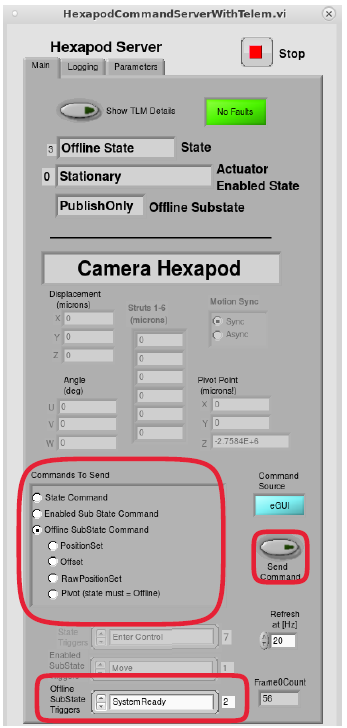
\includegraphics[width=1.79167in,height=\textheight]{jira_imgs/1024.png}

}
\hdashrule[0.5ex]{\textwidth}{1pt}{3mm}
  Expected Result \\
{\footnotesize
The system transitions from the OfflineState/PublishOnly substate to the
OfflineState/AvailableState substate.\\
\strut \\

}
\hdashrule[0.5ex]{\textwidth}{1pt}{3mm}
  Actual Result \\
{\footnotesize

}
\begin{tabular}{p{2cm}p{14cm}}
\toprule
Step 4 & Step Execution Status: \textbf{ Pass } \\ \hline
\end{tabular}
 Description \\
{\footnotesize
\textbf{SWITCHING TO DDS MODE}\\
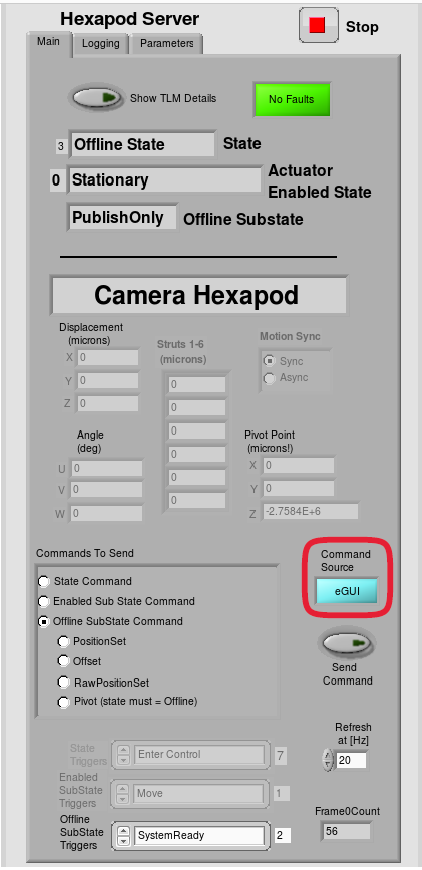
\includegraphics[width=1.6875in,height=\textheight]{jira_imgs/1025.png}If
the Command Source does not show DDS, go to the Parameters tab, select
DDS under the Command Source and click the Set Cmd Source button.\\
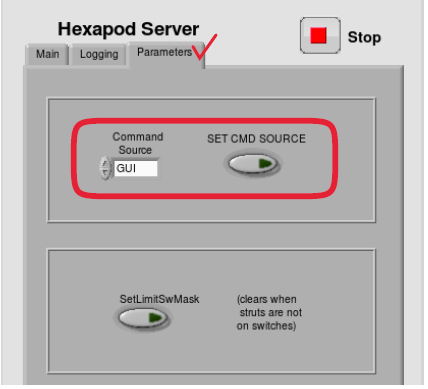
\includegraphics[width=2.34375in,height=\textheight]{jira_imgs/1026.png}\ul{\textbf{Note:}}\textbf{~If
the GUI is used after being set to DDS mode, the system will switch back
the Command Source to GUI and ignore any DDS commands. The Command
Source must show DDS in order to receive DDS commands.}

}
\hdashrule[0.5ex]{\textwidth}{1pt}{3mm}
  Expected Result \\
{\footnotesize
The system is capable of receiving/responding to DDS commands.

}
\hdashrule[0.5ex]{\textwidth}{1pt}{3mm}
  Actual Result \\
{\footnotesize

}
\begin{tabular}{p{2cm}p{14cm}}
\toprule
Step 5 & Step Execution Status: \textbf{ Pass } \\ \hline
\end{tabular}
 Description \\
{\footnotesize
\textbf{OFFLINESTATE -\textgreater{} STANDBYSTATE}\\
The system receives an enterControl State Transition command through
DDS.

}
\hdashrule[0.5ex]{\textwidth}{1pt}{3mm}
  Expected Result \\
{\footnotesize
The system transitions into the StandbyState and is capable of
receiving/responding to DDS commands.

}
\hdashrule[0.5ex]{\textwidth}{1pt}{3mm}
  Actual Result \\
{\footnotesize

}
\begin{tabular}{p{2cm}p{14cm}}
\toprule
Step 6 & Step Execution Status: \textbf{ Pass } \\ \hline
\end{tabular}
 Description \\
{\footnotesize
\textbf{STANDBYSTATE -\textgreater{} DISABLEDSTATE}\\
From the StandbyState, send a start command through the DDS.

}
\hdashrule[0.5ex]{\textwidth}{1pt}{3mm}
  Expected Result \\
{\footnotesize
The system transitions into DisabledState after receiving/responding to
DDS command and the wrapper in the PXI real time controller looks for
the configuration file.\\
\strut \\
If the configuration file is invalid or out of range, the system will
transition into a Fault State

}
\hdashrule[0.5ex]{\textwidth}{1pt}{3mm}
  Actual Result \\
{\footnotesize
Yes, the configuration was correctly loaded. No invalid configuration
file was tested.

}
\begin{tabular}{p{2cm}p{14cm}}
\toprule
Step 7 & Step Execution Status: \textbf{ Pass } \\ \hline
\end{tabular}
 Description \\
{\footnotesize
\textbf{DISABLEDSTATE -\textgreater{} ENABLEDSTATE}\\
From the DisabledState, send an enable state command through the DDS.\\
\textbf{}

}
\hdashrule[0.5ex]{\textwidth}{1pt}{3mm}
  Expected Result \\
{\footnotesize
The system transitions into the EnabledState/Stationary substate, the
motor drives are enabled, motor brakes are released and the system is
capable of receiving/responding to DDS commands.\\
\strut \\

}
\hdashrule[0.5ex]{\textwidth}{1pt}{3mm}
  Actual Result \\
{\footnotesize

}
\begin{tabular}{p{2cm}p{14cm}}
\toprule
Step 8 & Step Execution Status: \textbf{ Not Executed } \\ \hline
\end{tabular}
 Description \\
{\footnotesize
\textbf{FAULTSTATE}\\
If a Fault occurs in any of the other states, the system will
automatically transition to the Fault State. While in the Fault state,
send a clearError command through the DDS.\\
\ul{Note:} If the fault that occurs goes through the interlock system,
reset the safety relay switch and send a clearError command.

}
\hdashrule[0.5ex]{\textwidth}{1pt}{3mm}
  Expected Result \\
{\footnotesize
The system transitions back to the OfflineState/PublishOnly substate and
is not capable of receiving/responding to DDS commands. (Go back to Step
3)

}
\hdashrule[0.5ex]{\textwidth}{1pt}{3mm}
  Actual Result \\
{\footnotesize

}
\begin{tabular}{p{2cm}p{14cm}}
\toprule
Step 9 & Step Execution Status: \textbf{ Pass } \\ \hline
\end{tabular}
 Description \\
{\footnotesize
Verify that the thermal sensors are connected and producing telemetry
into the EFD.

}
\hdashrule[0.5ex]{\textwidth}{1pt}{3mm}
  Expected Result \\
{\footnotesize
All actuator temperatures are published to the EFD.

}
\hdashrule[0.5ex]{\textwidth}{1pt}{3mm}
  Actual Result \\
{\footnotesize
ESS CSC produces temperature data and data are ingested into the EFD.

}
\begin{tabular}{p{2cm}p{14cm}}
\toprule
Step 10 & Step Execution Status: \textbf{ Pass } \\ \hline
\end{tabular}
 Description \\
{\footnotesize
The following steps define what the Jupyter Notebook for this test case
implements. Executing the Jupyter notebook is the only actual command
and control step that needs to be executed.

}
\hdashrule[0.5ex]{\textwidth}{1pt}{3mm}
  Expected Result \\
{\footnotesize
The Jupyter notebook controls the system to run through the steps below.

}
\hdashrule[0.5ex]{\textwidth}{1pt}{3mm}
  Actual Result \\
{\footnotesize
Yes, all controls are done via Jupyternote books

}
\begin{tabular}{p{2cm}p{14cm}}
\toprule
Step 11 & Step Execution Status: \textbf{ Pass } \\ \hline
\end{tabular}
 Description \\
{\footnotesize
Verify all the telemetry is being ingested into the EFD.

}
\hdashrule[0.5ex]{\textwidth}{1pt}{3mm}
  Expected Result \\
{\footnotesize
All telemetry defined in the script is being ingested into the EFD.

}
\hdashrule[0.5ex]{\textwidth}{1pt}{3mm}
  Actual Result \\
{\footnotesize

}
\begin{tabular}{p{2cm}p{14cm}}
\toprule
Step 12 & Step Execution Status: \textbf{ Pass } \\ \hline
\end{tabular}
 Description \\
{\footnotesize
\textbf{{MOVE TEST}}\\
\textbf{Section 3.1.2 of the attached Software Acceptance Test
Procedure\\
Test Sequence \#1 - Synchronous PositionSet and Move Commands}\\
In enabled/stationary state, send a positionSet command of (0um, 0um,
200um, 0 deg, 0 deg, 0 deg, s).

}
\hdashrule[0.5ex]{\textwidth}{1pt}{3mm}
  Test Data \\
 {\footnotesize
\textbf{Deviation:~}Skip this step. positionSet and move command
replaced by new move command. Now, the hexapod starts movement directly
after receiving the command.

}
\hdashrule[0.5ex]{\textwidth}{1pt}{3mm}
  Expected Result \\
{\footnotesize
The hexapod does not move.

}
\hdashrule[0.5ex]{\textwidth}{1pt}{3mm}
  Actual Result \\
{\footnotesize

}
\begin{tabular}{p{2cm}p{14cm}}
\toprule
Step 13 & Step Execution Status: \textbf{ Pass } \\ \hline
\end{tabular}
 Description \\
{\footnotesize
With the synchronous button enabled and in enabled/stationary state,
send a positionSet command of (500um, -500um, 200um, 0.01deg, -0.015deg,
0deg).

}
\hdashrule[0.5ex]{\textwidth}{1pt}{3mm}
  Test Data \\
 {\footnotesize
\textbf{Deviation:~}Skip this step. positionSet and move command
replaced by new move command. Now, the hexapod starts movement directly
after receiving the command.

}
\hdashrule[0.5ex]{\textwidth}{1pt}{3mm}
  Expected Result \\
{\footnotesize
The hexapod does not move

}
\hdashrule[0.5ex]{\textwidth}{1pt}{3mm}
  Actual Result \\
{\footnotesize

}
\begin{tabular}{p{2cm}p{14cm}}
\toprule
Step 14 & Step Execution Status: \textbf{ Pass } \\ \hline
\end{tabular}
 Description \\
{\footnotesize
With the hexapod in in enabled/stationary state sync=True and send the
move command of (x= 500um,y= -500um, z=200um, u=0.01deg, v=-0.015deg,
w=0deg).

}
\hdashrule[0.5ex]{\textwidth}{1pt}{3mm}
  Expected Result \\
{\footnotesize
\begin{itemize}
\tightlist
\item
  The hexapod moves to (x= 500um,y= -500um, z=200um, u=0.01deg,
  v=-0.015deg, w=0deg)
\item
  Since the Hexapod is in synchronous mode, the actuators complete the
  move at nearly the same time.
\end{itemize}

}
\hdashrule[0.5ex]{\textwidth}{1pt}{3mm}
  Actual Result \\
{\footnotesize
Ok, tested here:\\
START- Camera Hexapod Integration Test -\/- LVV-T1992 Test Step 7 -
Starting time: 2021-06-03 19:35:40.503417 UTC\\
\strut \\

}
\begin{tabular}{p{2cm}p{14cm}}
\toprule
Step 15 & Step Execution Status: \textbf{ Pass } \\ \hline
\end{tabular}
 Description \\
{\footnotesize
Record the corresponding DDS events that were generated.

}
\hdashrule[0.5ex]{\textwidth}{1pt}{3mm}
  Expected Result \\
{\footnotesize
\begin{itemize}
\tightlist
\item
  The controllerState.enabledSubstate goes to MOVING\_POINT\_TO\_POINT
  when the move begins and STATIONARY when the move ends.
\item
  An inPosition event is generated when the move is complete
\end{itemize}

}
\hdashrule[0.5ex]{\textwidth}{1pt}{3mm}
  Actual Result \\
{\footnotesize
Ok, tested here:\\
START- Camera Hexapod Integration Test -\/- LVV-T1992 Test Step 7 -
Starting time: 2021-06-03 19:35:40.503417 UTC\\
\strut \\

}
\begin{tabular}{p{2cm}p{14cm}}
\toprule
Step 16 & Step Execution Status: \textbf{ Pass } \\ \hline
\end{tabular}
 Description \\
{\footnotesize
Wait 39 seconds.

}
\hdashrule[0.5ex]{\textwidth}{1pt}{3mm}
  Expected Result \\
{\footnotesize

}
\hdashrule[0.5ex]{\textwidth}{1pt}{3mm}
  Actual Result \\
{\footnotesize

}
\begin{tabular}{p{2cm}p{14cm}}
\toprule
Step 17 & Step Execution Status: \textbf{ Pass } \\ \hline
\end{tabular}
 Description \\
{\footnotesize
Record the corresponding thermal sensors and verify they are below 19
deg C. If they are above 19 deg C, wait until they are below 19 deg C to
perform the following steps.

}
\hdashrule[0.5ex]{\textwidth}{1pt}{3mm}
  Expected Result \\
{\footnotesize
All actuators are below 19 deg C.

}
\hdashrule[0.5ex]{\textwidth}{1pt}{3mm}
  Actual Result \\
{\footnotesize
Ok, tested here:\\
START- Camera Hexapod Integration Test -\/- LVV-T1992 Test Step 7 -
Starting time: 2021-06-03 19:35:40.503417 UTC

}
\begin{tabular}{p{2cm}p{14cm}}
\toprule
Step 18 & Step Execution Status: \textbf{ Pass } \\ \hline
\end{tabular}
 Description \\
{\footnotesize
\textbf{Section 3.1.2 of the attached Software Acceptance Test
Procedure\\
Test Sequence \#5 - Stop Commands}\\
In the enabled/stationary state, send a move command of (x=0um, y=0um,
z=5000um, u=0deg, v=0deg, w=0deg)

}
\hdashrule[0.5ex]{\textwidth}{1pt}{3mm}
  Expected Result \\
{\footnotesize
The hexapod doesn\textquotesingle t move.

}
\hdashrule[0.5ex]{\textwidth}{1pt}{3mm}
  Actual Result \\
{\footnotesize

}
\begin{tabular}{p{2cm}p{14cm}}
\toprule
Step 19 & Step Execution Status: \textbf{ Pass } \\ \hline
\end{tabular}
 Description \\
{\footnotesize
Wait 3s.

}
\hdashrule[0.5ex]{\textwidth}{1pt}{3mm}
  Expected Result \\
{\footnotesize

}
\hdashrule[0.5ex]{\textwidth}{1pt}{3mm}
  Actual Result \\
{\footnotesize

}
\begin{tabular}{p{2cm}p{14cm}}
\toprule
Step 20 & Step Execution Status: \textbf{ Pass } \\ \hline
\end{tabular}
 Description \\
{\footnotesize
Send a stop command.

}
\hdashrule[0.5ex]{\textwidth}{1pt}{3mm}
  Expected Result \\
{\footnotesize
The hexapod stops before reaching the previously commanded position

}
\hdashrule[0.5ex]{\textwidth}{1pt}{3mm}
  Actual Result \\
{\footnotesize

}
\begin{tabular}{p{2cm}p{14cm}}
\toprule
Step 21 & Step Execution Status: \textbf{ Pass } \\ \hline
\end{tabular}
 Description \\
{\footnotesize
Record the corresponding DDS events that were generated.

}
\hdashrule[0.5ex]{\textwidth}{1pt}{3mm}
  Expected Result \\
{\footnotesize
\begin{itemize}
\tightlist
\item
  The controllerState.enabledSubstate goes to CONTROLLED\_STOPPING when
  the stop is requested, then STATIONARY when the hexapod has halted.
\item
  In the EFD the codes for the EnabledSubstate are:

  \begin{itemize}
  \tightlist
  \item
    Stationary=0
  \item
    MovingPointToPoint=1
  \item
    SlewingOrTracking=2
  \item
    ControlledStopping=3
  \item
    Initializing=4
  \item
    Relative=5
  \item
    ConstantVelocity=6
  \end{itemize}
\item
  No inPosition event is generated.
\end{itemize}

}
\hdashrule[0.5ex]{\textwidth}{1pt}{3mm}
  Actual Result \\
{\footnotesize
For details See:\\
START- Camera Hexapod Integration Test -\/- LVV-T1992 -\/- Stop command
test -\/- Starting Time: 2021-06-03 20:02:36.549874\\
\strut \\
Hexapod started to move. Moved for 3s. Stopped as commanded.\\
Controlled\_Stop event generated in the EFD. No inPosition event
generated.\\
\strut \\

}
\begin{tabular}{p{2cm}p{14cm}}
\toprule
Step 22 & Step Execution Status: \textbf{ Pass } \\ \hline
\end{tabular}
 Description \\
{\footnotesize
Wait 39 seconds.

}
\hdashrule[0.5ex]{\textwidth}{1pt}{3mm}
  Expected Result \\
{\footnotesize

}
\hdashrule[0.5ex]{\textwidth}{1pt}{3mm}
  Actual Result \\
{\footnotesize

}
\begin{tabular}{p{2cm}p{14cm}}
\toprule
Step 23 & Step Execution Status: \textbf{ Pass } \\ \hline
\end{tabular}
 Description \\
{\footnotesize
Record the corresponding thermal sensors and verify they are below 19
deg C. If they are above 19 deg C, wait until they are below 19 deg C to
perform the following steps.

}
\hdashrule[0.5ex]{\textwidth}{1pt}{3mm}
  Expected Result \\
{\footnotesize
All actuators are below 19 deg C.

}
\hdashrule[0.5ex]{\textwidth}{1pt}{3mm}
  Actual Result \\
{\footnotesize
For details See:\\
START- Camera Hexapod Integration Test -\/- LVV-T1992 -\/- Stop command
test -\/- Starting Time: 2021-06-03 20:02:36.549874

}
\begin{tabular}{p{2cm}p{14cm}}
\toprule
Step 24 & Step Execution Status: \textbf{ Pass } \\ \hline
\end{tabular}
 Description \\
{\footnotesize
\textbf{Section 3.1.2 of the attached Software Acceptance Test
Procedure\\
Test Sequence \#9 - positionSet and moveLUT}\\
\strut \\
\textbf{Update: Test the "setCompensationMode" command.}\\
\strut \\
In enabled/stationary state, send a move command of (x=0um, y=0um,
z=800um, u=0deg, v=0deg, w=0deg)\\
\strut \\

}
\hdashrule[0.5ex]{\textwidth}{1pt}{3mm}
  Test Data \\
 {\footnotesize
\textbf{Deviation:} There is no "positionSet" and no "moveLUT" command
anymore. "positionSet" and "move" command replaced by new "move"
command. Now, the hexapod starts movement directly after receiving the
command. moveLUT is replaced by a "setCompensationMode".

}
\hdashrule[0.5ex]{\textwidth}{1pt}{3mm}
  Expected Result \\
{\footnotesize
The hexapod moves to the position (x=0um, y=0um, z=800um, u=0deg,
v=0deg, w=0deg) and, since we are moving in synchronous mode, the
actuators complete the move at nearly the same time.

}
\hdashrule[0.5ex]{\textwidth}{1pt}{3mm}
  Actual Result \\
{\footnotesize
Camera hexapod reached the commanded position

}
\begin{tabular}{p{2cm}p{14cm}}
\toprule
Step 25 & Step Execution Status: \textbf{ Pass } \\ \hline
\end{tabular}
 Description \\
{\footnotesize
Ensure that MTMount publishes the telescope elevation angle and
MTRotator publishes the rotation angle of the rotator. Either as real
components or through controllers simulating the components.

}
\hdashrule[0.5ex]{\textwidth}{1pt}{3mm}
  Expected Result \\
{\footnotesize
Published telescope elevation and rotator angle.

}
\hdashrule[0.5ex]{\textwidth}{1pt}{3mm}
  Actual Result \\
{\footnotesize
\textbf{Deviation:~}We are using the real components or the simulated
ones. The azimuth must also be published.\\
Rotator angle, elevation, and azimuth are published.

}
\begin{tabular}{p{2cm}p{14cm}}
\toprule
Step 26 & Step Execution Status: \textbf{ Pass } \\ \hline
\end{tabular}
 Description \\
{\footnotesize
In enabled/stationary state, set ~"setCompensationMode" command to
enable=True.

}
\hdashrule[0.5ex]{\textwidth}{1pt}{3mm}
  Expected Result \\
{\footnotesize
The hexapod does not move and the
~MTHexapod.command\_setCompensationMode appears as true in the EFD.\\
\strut \\
logevent\_compensatedPosition is sent to the EFD.\\
\strut \\

}
\hdashrule[0.5ex]{\textwidth}{1pt}{3mm}
  Actual Result \\
{\footnotesize
\begin{verbatim}
Deviation: The hexapod is expected to move to the compensated position. 
This is what happened. The hexapod moved to the compensated position.
Here are the differences from the notebook
Predicted LUT compensation:
     -0.93    -652.98     295.56      -0.02       0.00       0.00
Uncompensated position
      0.00       0.00     800.00      0.000000   0.000000   0.000000    2021-07-13 19:45:18.343772928
Compensated position
     -0.93    -652.98    1095.56      -0.017752   0.000000   0.000000    2021-07-13 19:53:08.232006656
\end{verbatim}

\hfill\break
Attached is the result from the EFD for the setCompensationMode event
and the positions of the actuators\\
\strut \\
\strut \\

}
\begin{tabular}{p{2cm}p{14cm}}
\toprule
Step 27 & Step Execution Status: \textbf{ Pass } \\ \hline
\end{tabular}
 Description \\
{\footnotesize
In enabled/stationary state, send a move command of (0um, 0um, 800um,
0deg, 0deg, 0deg)

}
\hdashrule[0.5ex]{\textwidth}{1pt}{3mm}
  Expected Result \\
{\footnotesize
The hexapod moves to a slightly different position than (0um, 0um,
800um, 0deg, 0deg, 0deg) and, since we are moving in synchronous mode,
the actuators complete the move at nearly the same time.

}
\hdashrule[0.5ex]{\textwidth}{1pt}{3mm}
  Actual Result \\
{\footnotesize
This failed before:\\
\href{https://jira.lsstcorp.org/browse/DM-29692}{DM-29692~}Camera
MThexapod CompensationMode does not work\\
\strut \\
is a duplicate of\\
\strut \\
\href{https://jira.lsstcorp.org/browse/DM-29423}{DM-29423} {MTHexapod
moves can be delayed or lost if compensation mode is enabled}\\
\strut \\
{As a consequence, a software update was performed.}\\
{to~}

\begin{itemize}
\tightlist
\item
  ts\_hexrotcomm v0.18.0 ~
\item
  ts\_mthexapod v0.16.0
\end{itemize}

\hfill\break
This works now with deviation. See step above.

}
\begin{tabular}{p{2cm}p{14cm}}
\toprule
Step 28 & Step Execution Status: \textbf{ Pass } \\ \hline
\end{tabular}
 Description \\
{\footnotesize
Check if there are any different events between move with and without
setCompensationMode=True. Check the movement in the EFD use:\\
Compare logevent\_compensatedPosition to logevent\_uncompensatedPosition

}
\hdashrule[0.5ex]{\textwidth}{1pt}{3mm}
  Expected Result \\
{\footnotesize
The changes are expected according to this table:\\
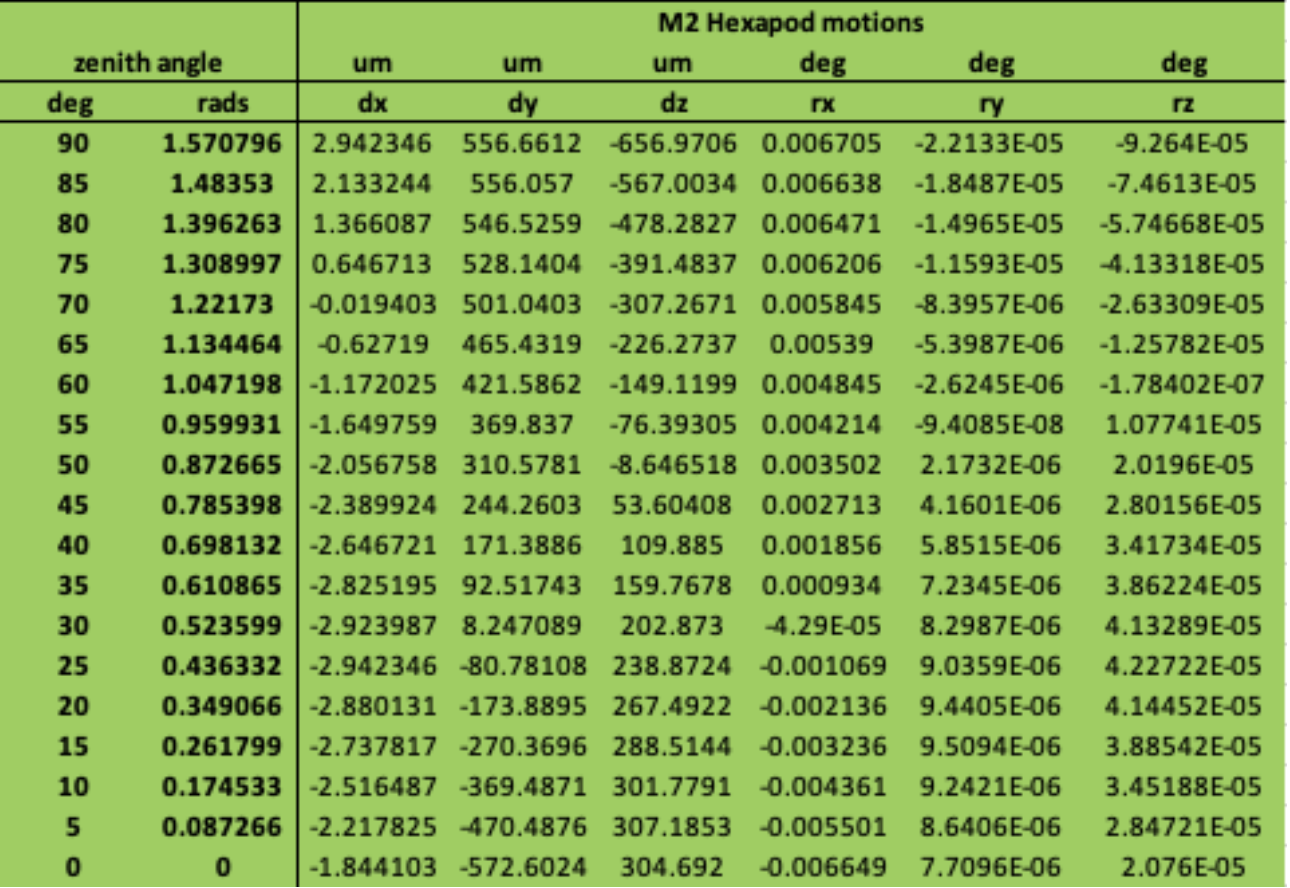
\includegraphics[width=1.5625in,height=\textheight]{jira_imgs/1620.png}\\

}
\hdashrule[0.5ex]{\textwidth}{1pt}{3mm}
  Actual Result \\
{\footnotesize
Yes, there is a difference between moving with and without compensation
mode activated.\\
The difference corresponds to the predicted difference\\
\strut \\
Predicted LUT compensation:\\
-0.93 -652.98 295.56 -0.02 0.00 0.00\\
Uncompensated position\\
0.00 0.00 800.00 0.000000 0.000000 0.000000 2021-07-13
19:45:18.343772928\\
Compensated position\\
-0.93 -652.98 1095.56 -0.017752 0.000000 0.000000 2021-07-13
19:53:08.232006656\\
\textbf{\hfill\break
Note: Check which table is actually used. Here the M2table is attached.
Do camera hexapod and M2 have the same tables for testing?}

}
\begin{tabular}{p{2cm}p{14cm}}
\toprule
Step 29 & Step Execution Status: \textbf{ Pass } \\ \hline
\end{tabular}
 Description \\
{\footnotesize
In enabled/stationary state, send a move command of (0um, 0um, 800um,
0deg, 0deg, 0deg)

}
\hdashrule[0.5ex]{\textwidth}{1pt}{3mm}
  Expected Result \\
{\footnotesize
The hexapod does not move since it stayed in compensationMode.

}
\hdashrule[0.5ex]{\textwidth}{1pt}{3mm}
  Actual Result \\
{\footnotesize
Confirmed. The hexapod does not move to a different position when
sending the same command again. The hexapod stays in the compensated
position.

}
\begin{tabular}{p{2cm}p{14cm}}
\toprule
Step 30 & Step Execution Status: \textbf{ Pass } \\ \hline
\end{tabular}
 Description \\
{\footnotesize
Wait 39 seconds.

}
\hdashrule[0.5ex]{\textwidth}{1pt}{3mm}
  Expected Result \\
{\footnotesize

}
\hdashrule[0.5ex]{\textwidth}{1pt}{3mm}
  Actual Result \\
{\footnotesize

}
\begin{tabular}{p{2cm}p{14cm}}
\toprule
Step 31 & Step Execution Status: \textbf{ Pass } \\ \hline
\end{tabular}
 Description \\
{\footnotesize
Record the corresponding thermal sensors and verify they are below 19
deg C. If they are above 19 deg C, wait until they are below 19 deg C to
perform the following steps.

}
\hdashrule[0.5ex]{\textwidth}{1pt}{3mm}
  Expected Result \\
{\footnotesize
All actuators are below 19 deg C.

}
\hdashrule[0.5ex]{\textwidth}{1pt}{3mm}
  Actual Result \\
{\footnotesize
Thermal sensors are below 19 deg

}
\begin{tabular}{p{2cm}p{14cm}}
\toprule
Step 32 & Step Execution Status: \textbf{ Pass } \\ \hline
\end{tabular}
 Description \\
{\footnotesize
{\textbf{OFFSET TEST}}\\
\textbf{Section 3.1.2 of the attached Software Acceptance Test
Procedure\\
Test Sequence \#4 - Synchronous Offset and Move Commands}\\
In enabled/stationary state, send a move command of (x=500um, y=800um,
z=200um, u=0deg, v=0deg, w=0deg)

}
\hdashrule[0.5ex]{\textwidth}{1pt}{3mm}
  Test Data \\
 {\footnotesize
\textbf{Deviation:} There is no positionSet command anymore. positionSet
and move command replaced by new move command. Now, the hexapod starts
movement directly after receiving the command.\\
\strut \\

}
\hdashrule[0.5ex]{\textwidth}{1pt}{3mm}
  Expected Result \\
{\footnotesize
\begin{itemize}
\tightlist
\item
  The hexapod moves to (x=500um, y=800um, z=200um, u=0deg, v=0deg,
  w=0deg)
\item
  Since the Hexapod is in synchronous mode, the actuators complete the
  move at nearly the same time.
\end{itemize}

}
\hdashrule[0.5ex]{\textwidth}{1pt}{3mm}
  Actual Result \\
{\footnotesize
Hexapod arrived to (500um, 800um, 200um, 0deg, 0deg, 0deg).\\
For details see: START- Camera Hexapod Integration Test -\/- LVV-T1992
-\/- offset command test -\/- Starting time: 2021-06-03 20:50:56.089773
UTC

}
\begin{tabular}{p{2cm}p{14cm}}
\toprule
Step 33 & Step Execution Status: \textbf{ Pass } \\ \hline
\end{tabular}
 Description \\
{\footnotesize
In enabled/stationary state, send an offset command of (0um, 0um, 500um,
0deg, 0deg, 0deg).

}
\hdashrule[0.5ex]{\textwidth}{1pt}{3mm}
  Expected Result \\
{\footnotesize
\begin{itemize}
\tightlist
\item
  The hexapod moves only 500um in Z from the previous position
\item
  The actuators complete the move at nearly the same time.
\end{itemize}

}
\hdashrule[0.5ex]{\textwidth}{1pt}{3mm}
  Actual Result \\
{\footnotesize

}
\begin{tabular}{p{2cm}p{14cm}}
\toprule
Step 34 & Step Execution Status: \textbf{ Pass } \\ \hline
\end{tabular}
 Description \\
{\footnotesize
Send a move command.~

}
\hdashrule[0.5ex]{\textwidth}{1pt}{3mm}
  Test Data \\
 {\footnotesize
\textbf{Deviation:} Skip this step. The Hexapod has already moved.

}
\hdashrule[0.5ex]{\textwidth}{1pt}{3mm}
  Expected Result \\
{\footnotesize
\begin{itemize}
\tightlist
\item
  The hexapod moves only 500um in Z from the previous position
\item
  The actuators complete the move at nearly the same time.
\end{itemize}

}
\hdashrule[0.5ex]{\textwidth}{1pt}{3mm}
  Actual Result \\
{\footnotesize

}
\begin{tabular}{p{2cm}p{14cm}}
\toprule
Step 35 & Step Execution Status: \textbf{ Pass } \\ \hline
\end{tabular}
 Description \\
{\footnotesize
Wait 39s.

}
\hdashrule[0.5ex]{\textwidth}{1pt}{3mm}
  Expected Result \\
{\footnotesize

}
\hdashrule[0.5ex]{\textwidth}{1pt}{3mm}
  Actual Result \\
{\footnotesize

}
\begin{tabular}{p{2cm}p{14cm}}
\toprule
Step 36 & Step Execution Status: \textbf{ Pass } \\ \hline
\end{tabular}
 Description \\
{\footnotesize
Record the corresponding DDS events that were generated.

}
\hdashrule[0.5ex]{\textwidth}{1pt}{3mm}
  Expected Result \\
{\footnotesize
\begin{itemize}
\tightlist
\item
  The controllerState.enabledSubstate goes to MOVING\_POINT\_TO\_POINT
  when the move begins and STATIONARY when the move ends
\item
  The inPosition event is True when the move finishes
\item
  The inPosition event is False when the enabledSubstate goes back to
  STATIONARY.
\end{itemize}

}
\hdashrule[0.5ex]{\textwidth}{1pt}{3mm}
  Actual Result \\
{\footnotesize
Move and offset correctly executed.\\
For details see: START- Camera Hexapod Integration Test -\/- LVV-T1992
-\/- offset command test -\/- Starting time: 2021-06-03 20:50:56.089773
UTC

}
\begin{tabular}{p{2cm}p{14cm}}
\toprule
Step 37 & Step Execution Status: \textbf{ Pass } \\ \hline
\end{tabular}
 Description \\
{\footnotesize
\textbf{Section 3.1.2 of the attached Software Acceptance Test
Procedure\\
Test Sequence \#2 -Pivot, PositionSet and Move Commands}\\
In enabled/stationary state, send a move command of
(x=2000um,y=-3500um,z=200um,u=0.01deg,v=-0.05deg, w=0.002deg,sync=true)

}
\hdashrule[0.5ex]{\textwidth}{1pt}{3mm}
  Test Data \\
 {\footnotesize
\textbf{Deviation:} Determine where the original pivot point is before
sending a pivot command of (0, 0, 0).\\
Record any offset commands necessary to test before sending the move
command.

}
\hdashrule[0.5ex]{\textwidth}{1pt}{3mm}
  Expected Result \\
{\footnotesize
The hexapod moves to the commanded position

}
\hdashrule[0.5ex]{\textwidth}{1pt}{3mm}
  Actual Result \\
{\footnotesize
\begin{verbatim}
INFO:Script:START- Camera Hexapod Integration Test -- LVV-T1600 Pivot test - Moving to testing position- Starting time: 2021-07-07 21:41:28.497169 UTC
\end{verbatim}

\begin{verbatim}
pivot at (0, 0, -2758400) microns 
maxXY =  11400.0 microns, maxZ=  13100.0  microns
maxUV =  0.36 deg, maxW=  0.1  deg
\end{verbatim}

\begin{verbatim}
Hex position in X,Y,Z,U,V,W
   1999.29    -3500.15      199.85        0.01       -0.05        0.00  

Hexapod calibrated actuator positions in um:
  -1534.55    -1185.38     2597.15     -905.41    -1476.09     1602.86  
\end{verbatim}

\begin{verbatim}
\end{verbatim}

}
\begin{tabular}{p{2cm}p{14cm}}
\toprule
Step 38 & Step Execution Status: \textbf{ Pass } \\ \hline
\end{tabular}
 Description \\
{\footnotesize
In the enabled/stationary state, send a pivot command of (0,0,0).

}
\hdashrule[0.5ex]{\textwidth}{1pt}{3mm}
  Expected Result \\
{\footnotesize
The actuator positions do not change but the hexapod position changes to
account for the new pivot point.

}
\hdashrule[0.5ex]{\textwidth}{1pt}{3mm}
  Actual Result \\
{\footnotesize
\begin{verbatim}
INFO:Script:START- Camera Hexapod Integration Test -- LVV-T1600 Pivot test - Pivot point set to (0,0,0)- Starting time: 2021-07-07 21:41:58.488606 UTC
\end{verbatim}

\begin{verbatim}
pivot at (0, 0, 0) microns 
maxXY =  11400.0 microns, maxZ=  13100.0  microns
maxUV =  0.36 deg, maxW=  0.1  deg
Hex position in X,Y,Z,U,V,W
\end{verbatim}

\begin{verbatim}
Hex position in X,Y,Z,U,V,W
   -407.78    -3981.80      198.75        0.01       -0.05        0.00  

Hexapod calibrated actuator positions in um:
  -1534.50    -1185.38     2597.17     -905.41    -1476.21     1602.94  
\end{verbatim}

}
\begin{tabular}{p{2cm}p{14cm}}
\toprule
Step 39 & Step Execution Status: \textbf{ Pass } \\ \hline
\end{tabular}
 Description \\
{\footnotesize
In the enabled/stationary state, send again the move command of
(x=2000um, y=-3500um, z=200um, u=0.01deg, v=-0.05deg,
w=0.002deg,sync=true)

}
\hdashrule[0.5ex]{\textwidth}{1pt}{3mm}
  Test Data \\
 {\footnotesize
\textbf{Deviation:} Record any offset commands necessary to test before
sending the move command.\\
\strut \\

}
\hdashrule[0.5ex]{\textwidth}{1pt}{3mm}
  Expected Result \\
{\footnotesize
Confirm the hexapod moves to the commanded position and the actuators
change position to account for the new pivot point. Position values in
the EFD appear different.

}
\hdashrule[0.5ex]{\textwidth}{1pt}{3mm}
  Actual Result \\
{\footnotesize
INFO:Script:START- Camera Hexapod Integration Test -\/- LVV-T1600 move
to ~(x=2000,y=-3500,z=200,u=0.01,v=-0.05,w=0.002,sync=True) again- Pivot
test - Starting time: 2021-07-07 21:41:58.488606 UTC

\begin{verbatim}
Hex position in X,Y,Z,U,V,W
   2000.54    -3499.86      200.15        0.01       -0.05        0.00  

Hexapod calibrated actuator positions in um:
  -2596.90      153.42     2323.62    -1966.31     -136.49     1328.17  
\end{verbatim}

\hfill\break
The logevent is created and correctly reflected in the EFD.\\
{The issued command expected under e.g.
"lsst.sal.MTHexapod.command\_pivot.x" is not updated. Look for
"lsst.sal.MTHexapod.command\_setPivot.x" and it works!}{\hfill\break
}

}
\begin{tabular}{p{2cm}p{14cm}}
\toprule
Step 40 & Step Execution Status: \textbf{ Pass } \\ \hline
\end{tabular}
 Description \\
{\footnotesize
Wait 39s.

}
\hdashrule[0.5ex]{\textwidth}{1pt}{3mm}
  Expected Result \\
{\footnotesize

}
\hdashrule[0.5ex]{\textwidth}{1pt}{3mm}
  Actual Result \\
{\footnotesize

}
\begin{tabular}{p{2cm}p{14cm}}
\toprule
Step 41 & Step Execution Status: \textbf{ Not Executed } \\ \hline
\end{tabular}
 Description \\
{\footnotesize
\textbf{{CONFIGURE LIMITS TEST}}\\
\textbf{Section 3.1.2 of the attached Software Acceptance Test
Procedure\\
Test Sequence \#6 - configureLimits Command}\\
In enabled/stationary state, send a configureLimits command of (12000um,
-1000um, 1000um, 0.1, -0.1, 0.05)

}
\hdashrule[0.5ex]{\textwidth}{1pt}{3mm}
  Test Data \\
 {\footnotesize
\textbf{Deviation:} Skip complete test. This test uses an obsolete
command. The configuration is now done before and should not be changed
this state

}
\hdashrule[0.5ex]{\textwidth}{1pt}{3mm}
  Expected Result \\
{\footnotesize
The command is rejected for being outside acceptable limits.

}
\hdashrule[0.5ex]{\textwidth}{1pt}{3mm}
  Actual Result \\
{\footnotesize

}
\begin{tabular}{p{2cm}p{14cm}}
\toprule
Step 42 & Step Execution Status: \textbf{ Not Executed } \\ \hline
\end{tabular}
 Description \\
{\footnotesize
In enabled/stationary state, send a configureLimits command of (1000um,
-1000um, 1000um, 0.1, -0.1, 0.05)

}
\hdashrule[0.5ex]{\textwidth}{1pt}{3mm}
  Expected Result \\
{\footnotesize
The command is accepted.

}
\hdashrule[0.5ex]{\textwidth}{1pt}{3mm}
  Actual Result \\
{\footnotesize

}
\begin{tabular}{p{2cm}p{14cm}}
\toprule
Step 43 & Step Execution Status: \textbf{ Not Executed } \\ \hline
\end{tabular}
 Description \\
{\footnotesize
In enabled/stationary state, send a positionSet command of (1200um, 0um,
200um, 0deg, 0deg, 0deg)

}
\hdashrule[0.5ex]{\textwidth}{1pt}{3mm}
  Expected Result \\
{\footnotesize
The command is rejected for being outside of range limits

}
\hdashrule[0.5ex]{\textwidth}{1pt}{3mm}
  Actual Result \\
{\footnotesize

}
\begin{tabular}{p{2cm}p{14cm}}
\toprule
Step 44 & Step Execution Status: \textbf{ Not Executed } \\ \hline
\end{tabular}
 Description \\
{\footnotesize
In enabled/stationary state, send a positionSet command of (990um,
990um, 200um, 0deg, 0deg, 0deg)

}
\hdashrule[0.5ex]{\textwidth}{1pt}{3mm}
  Expected Result \\
{\footnotesize
The command is rejected for being outside of range limits.

}
\hdashrule[0.5ex]{\textwidth}{1pt}{3mm}
  Actual Result \\
{\footnotesize

}
\begin{tabular}{p{2cm}p{14cm}}
\toprule
Step 45 & Step Execution Status: \textbf{ Not Executed } \\ \hline
\end{tabular}
 Description \\
{\footnotesize
In enabled/stationary state, send a positionSet command of (500um,
500um, 200um, 0deg, 0.1 deg, 0.01deg)

}
\hdashrule[0.5ex]{\textwidth}{1pt}{3mm}
  Expected Result \\
{\footnotesize
The command is accepted.

}
\hdashrule[0.5ex]{\textwidth}{1pt}{3mm}
  Actual Result \\
{\footnotesize

}
\begin{tabular}{p{2cm}p{14cm}}
\toprule
Step 46 & Step Execution Status: \textbf{ Not Executed } \\ \hline
\end{tabular}
 Description \\
{\footnotesize
Send a move command.

}
\hdashrule[0.5ex]{\textwidth}{1pt}{3mm}
  Expected Result \\
{\footnotesize
The previously accepted command is executed.

}
\hdashrule[0.5ex]{\textwidth}{1pt}{3mm}
  Actual Result \\
{\footnotesize

}
\begin{tabular}{p{2cm}p{14cm}}
\toprule
Step 47 & Step Execution Status: \textbf{ Not Executed } \\ \hline
\end{tabular}
 Description \\
{\footnotesize
Record the DDS events that were generated.

}
\hdashrule[0.5ex]{\textwidth}{1pt}{3mm}
  Expected Result \\
{\footnotesize
The change is reflected in the settingsApplied event and the EUI.

}
\hdashrule[0.5ex]{\textwidth}{1pt}{3mm}
  Actual Result \\
{\footnotesize

}
\begin{tabular}{p{2cm}p{14cm}}
\toprule
Step 48 & Step Execution Status: \textbf{ Not Executed } \\ \hline
\end{tabular}
 Description \\
{\footnotesize
{\textbf{CONFIGURE ACCELERATION TEST}}\\
\textbf{Section 3.1.2 of the attached Software Acceptance Test
Procedure\\
Test Sequence \#7 - configureAcceleration Command}\\
In enabled/stationary state, at a position of (0, 0, 0, 0, 0, 0) with
the velocity and acceleration values set to their nominal values, send a
positionSet command of (0um, 0um, 4900um, 0 deg, 0 deg, 0 deg, s).

}
\hdashrule[0.5ex]{\textwidth}{1pt}{3mm}
  Test Data \\
 {\footnotesize
\textbf{Deviation:} Skip complete test. This test uses an obsolete
command. The configuration is now done before and should not be changed
this state

}
\hdashrule[0.5ex]{\textwidth}{1pt}{3mm}
  Expected Result \\
{\footnotesize
The hexapod doesn\textquotesingle t move.

}
\hdashrule[0.5ex]{\textwidth}{1pt}{3mm}
  Actual Result \\
{\footnotesize

}
\begin{tabular}{p{2cm}p{14cm}}
\toprule
Step 49 & Step Execution Status: \textbf{ Not Executed } \\ \hline
\end{tabular}
 Description \\
{\footnotesize
Send a move command.

}
\hdashrule[0.5ex]{\textwidth}{1pt}{3mm}
  Expected Result \\
{\footnotesize
The move takes approximately 9 seconds to complete.

}
\hdashrule[0.5ex]{\textwidth}{1pt}{3mm}
  Actual Result \\
{\footnotesize

}
\begin{tabular}{p{2cm}p{14cm}}
\toprule
Step 50 & Step Execution Status: \textbf{ Not Executed } \\ \hline
\end{tabular}
 Description \\
{\footnotesize
Send a configureAcceleration command of 1000.

}
\hdashrule[0.5ex]{\textwidth}{1pt}{3mm}
  Expected Result \\
{\footnotesize
~Confirm command is rejected for being outside of acceptable limits.

}
\hdashrule[0.5ex]{\textwidth}{1pt}{3mm}
  Actual Result \\
{\footnotesize

}
\begin{tabular}{p{2cm}p{14cm}}
\toprule
Step 51 & Step Execution Status: \textbf{ Not Executed } \\ \hline
\end{tabular}
 Description \\
{\footnotesize
Send a configureAcceleration command of 100.

}
\hdashrule[0.5ex]{\textwidth}{1pt}{3mm}
  Expected Result \\
{\footnotesize
The command is accepted.~

}
\hdashrule[0.5ex]{\textwidth}{1pt}{3mm}
  Actual Result \\
{\footnotesize

}
\begin{tabular}{p{2cm}p{14cm}}
\toprule
Step 52 & Step Execution Status: \textbf{ Not Executed } \\ \hline
\end{tabular}
 Description \\
{\footnotesize
In enabled/stationary state, send a postionSet command of (0um, 0um,
0um, 0 deg, 0 deg, 0 deg, s).

}
\hdashrule[0.5ex]{\textwidth}{1pt}{3mm}
  Expected Result \\
{\footnotesize
The hexapod doesn\textquotesingle t move.

}
\hdashrule[0.5ex]{\textwidth}{1pt}{3mm}
  Actual Result \\
{\footnotesize

}
\begin{tabular}{p{2cm}p{14cm}}
\toprule
Step 53 & Step Execution Status: \textbf{ Not Executed } \\ \hline
\end{tabular}
 Description \\
{\footnotesize
Send a move command.~

}
\hdashrule[0.5ex]{\textwidth}{1pt}{3mm}
  Expected Result \\
{\footnotesize
It takes approximately 13 seconds to complete the commanded move with
the reduced acceleration value.

}
\hdashrule[0.5ex]{\textwidth}{1pt}{3mm}
  Actual Result \\
{\footnotesize

}
\begin{tabular}{p{2cm}p{14cm}}
\toprule
Step 54 & Step Execution Status: \textbf{ Not Executed } \\ \hline
\end{tabular}
 Description \\
{\footnotesize
Send a configureAcceleration command of 500 to return the acceleration
limit to its nominal value.

}
\hdashrule[0.5ex]{\textwidth}{1pt}{3mm}
  Expected Result \\
{\footnotesize
The command is accepted.

}
\hdashrule[0.5ex]{\textwidth}{1pt}{3mm}
  Actual Result \\
{\footnotesize

}
\begin{tabular}{p{2cm}p{14cm}}
\toprule
Step 55 & Step Execution Status: \textbf{ Not Executed } \\ \hline
\end{tabular}
 Description \\
{\footnotesize
Record the corresponding DDS events that were generated.

}
\hdashrule[0.5ex]{\textwidth}{1pt}{3mm}
  Expected Result \\
{\footnotesize
The change is reflected in the settingsApplied event and the EUI.

}
\hdashrule[0.5ex]{\textwidth}{1pt}{3mm}
  Actual Result \\
{\footnotesize

}
\begin{tabular}{p{2cm}p{14cm}}
\toprule
Step 56 & Step Execution Status: \textbf{ Not Executed } \\ \hline
\end{tabular}
 Description \\
{\footnotesize
\textbf{{CONFIGURE VELOCITY TEST}}\\
\textbf{Section 3.1.2 of the attached Software Acceptance Test
Procedure\\
Test Sequence \#8 - configureVelocity Command}\\
In enabled/stationary state, at a position of (0, 0, 0, 0, 0, 0), send a
configureVelocity command of (10000, .01, 100, .01).

}
\hdashrule[0.5ex]{\textwidth}{1pt}{3mm}
  Test Data \\
 {\footnotesize
\textbf{Deviation:} Skip complete test. This test uses an obsolete
command. The configuration is now done before and should not be changed
this state

}
\hdashrule[0.5ex]{\textwidth}{1pt}{3mm}
  Expected Result \\
{\footnotesize
This command is rejected for being outside of acceptable limits.

}
\hdashrule[0.5ex]{\textwidth}{1pt}{3mm}
  Actual Result \\
{\footnotesize

}
\begin{tabular}{p{2cm}p{14cm}}
\toprule
Step 57 & Step Execution Status: \textbf{ Not Executed } \\ \hline
\end{tabular}
 Description \\
{\footnotesize
In enabled/stationary state, send a configureVelocity command of (100,
.01, 200, .01).~

}
\hdashrule[0.5ex]{\textwidth}{1pt}{3mm}
  Expected Result \\
{\footnotesize
This command is accepted.

}
\hdashrule[0.5ex]{\textwidth}{1pt}{3mm}
  Actual Result \\
{\footnotesize

}
\begin{tabular}{p{2cm}p{14cm}}
\toprule
Step 58 & Step Execution Status: \textbf{ Not Executed } \\ \hline
\end{tabular}
 Description \\
{\footnotesize
In enabled/stationary state, send a positionSet command of (0, 0um,
2000um, 0 deg, 0 deg, 0 deg, s).

}
\hdashrule[0.5ex]{\textwidth}{1pt}{3mm}
  Expected Result \\
{\footnotesize
The command is accepted

}
\hdashrule[0.5ex]{\textwidth}{1pt}{3mm}
  Actual Result \\
{\footnotesize

}
\begin{tabular}{p{2cm}p{14cm}}
\toprule
Step 59 & Step Execution Status: \textbf{ Not Executed } \\ \hline
\end{tabular}
 Description \\
{\footnotesize
Send a move command.~

}
\hdashrule[0.5ex]{\textwidth}{1pt}{3mm}
  Expected Result \\
{\footnotesize
It takes approximately 20 seconds to complete the commanded move.

}
\hdashrule[0.5ex]{\textwidth}{1pt}{3mm}
  Actual Result \\
{\footnotesize

}
\begin{tabular}{p{2cm}p{14cm}}
\toprule
Step 60 & Step Execution Status: \textbf{ Not Executed } \\ \hline
\end{tabular}
 Description \\
{\footnotesize
In enabled/stationary state, send a configureVelocity command of (100,
.01, 100, .01).~

}
\hdashrule[0.5ex]{\textwidth}{1pt}{3mm}
  Expected Result \\
{\footnotesize
This command is accepted.

}
\hdashrule[0.5ex]{\textwidth}{1pt}{3mm}
  Actual Result \\
{\footnotesize

}
\begin{tabular}{p{2cm}p{14cm}}
\toprule
Step 61 & Step Execution Status: \textbf{ Not Executed } \\ \hline
\end{tabular}
 Description \\
{\footnotesize
In enabled/stationary state, send an offset command of (0, 0um, 2000um,
0 deg, 0 deg, 0 deg).

}
\hdashrule[0.5ex]{\textwidth}{1pt}{3mm}
  Expected Result \\
{\footnotesize
This command is accepted

}
\hdashrule[0.5ex]{\textwidth}{1pt}{3mm}
  Actual Result \\
{\footnotesize

}
\begin{tabular}{p{2cm}p{14cm}}
\toprule
Step 62 & Step Execution Status: \textbf{ Not Executed } \\ \hline
\end{tabular}
 Description \\
{\footnotesize
Send a move command.~

}
\hdashrule[0.5ex]{\textwidth}{1pt}{3mm}
  Expected Result \\
{\footnotesize
It takes approximately 40 seconds to complete the commanded move.

}
\hdashrule[0.5ex]{\textwidth}{1pt}{3mm}
  Actual Result \\
{\footnotesize

}
\begin{tabular}{p{2cm}p{14cm}}
\toprule
Step 63 & Step Execution Status: \textbf{ Not Executed } \\ \hline
\end{tabular}
 Description \\
{\footnotesize
Record the corresponding DDS events that were generated:

}
\hdashrule[0.5ex]{\textwidth}{1pt}{3mm}
  Expected Result \\
{\footnotesize
The change is reflected in the settingsApplied event and the EUI.

}
\hdashrule[0.5ex]{\textwidth}{1pt}{3mm}
  Actual Result \\
{\footnotesize

}
\begin{tabular}{p{2cm}p{14cm}}
\toprule
Step 64 & Step Execution Status: \textbf{ Pass } \\ \hline
\end{tabular}
 Description \\
{\footnotesize
\textbf{Section 3.3.2 of the attached Software Acceptance Test Procedure
Hexapod Action on State Commands}\\
In the Offline/PublishOnly state, send all commands

}
\hdashrule[0.5ex]{\textwidth}{1pt}{3mm}
  Expected Result \\
{\footnotesize
There is no change and command is rejected.

}
\hdashrule[0.5ex]{\textwidth}{1pt}{3mm}
  Actual Result \\
{\footnotesize

}
\begin{tabular}{p{2cm}p{14cm}}
\toprule
Step 65 & Step Execution Status: \textbf{ Not Executed } \\ \hline
\end{tabular}
 Description \\
{\footnotesize
In the Offline/Available state, send an enterControl command

}
\hdashrule[0.5ex]{\textwidth}{1pt}{3mm}
  Expected Result \\
{\footnotesize
The system enters the Standby state.

}
\hdashrule[0.5ex]{\textwidth}{1pt}{3mm}
  Actual Result \\
{\footnotesize

}
\begin{tabular}{p{2cm}p{14cm}}
\toprule
Step 66 & Step Execution Status: \textbf{ Not Executed } \\ \hline
\end{tabular}
 Description \\
{\footnotesize
In the Standby state, send any command except start or exitControl

}
\hdashrule[0.5ex]{\textwidth}{1pt}{3mm}
  Expected Result \\
{\footnotesize
There is no change and command is rejected.

}
\hdashrule[0.5ex]{\textwidth}{1pt}{3mm}
  Actual Result \\
{\footnotesize

}
\begin{tabular}{p{2cm}p{14cm}}
\toprule
Step 67 & Step Execution Status: \textbf{ Not Executed } \\ \hline
\end{tabular}
 Description \\
{\footnotesize
In the Standby state, send an exitControl command.

}
\hdashrule[0.5ex]{\textwidth}{1pt}{3mm}
  Expected Result \\
{\footnotesize
The system transitions into the Offline/Available state.

}
\hdashrule[0.5ex]{\textwidth}{1pt}{3mm}
  Actual Result \\
{\footnotesize

}
\begin{tabular}{p{2cm}p{14cm}}
\toprule
Step 68 & Step Execution Status: \textbf{ Not Executed } \\ \hline
\end{tabular}
 Description \\
{\footnotesize
In the Standby state, send a start command.

}
\hdashrule[0.5ex]{\textwidth}{1pt}{3mm}
  Expected Result \\
{\footnotesize
The system transitions into the Disabled state.

}
\hdashrule[0.5ex]{\textwidth}{1pt}{3mm}
  Actual Result \\
{\footnotesize

}
\begin{tabular}{p{2cm}p{14cm}}
\toprule
Step 69 & Step Execution Status: \textbf{ Not Executed } \\ \hline
\end{tabular}
 Description \\
{\footnotesize
In the Disabled state, send any command except for the enabled or
standby command.

}
\hdashrule[0.5ex]{\textwidth}{1pt}{3mm}
  Expected Result \\
{\footnotesize
There is no change and the command is rejected.

}
\hdashrule[0.5ex]{\textwidth}{1pt}{3mm}
  Actual Result \\
{\footnotesize

}
\begin{tabular}{p{2cm}p{14cm}}
\toprule
Step 70 & Step Execution Status: \textbf{ Pass } \\ \hline
\end{tabular}
 Description \\
{\footnotesize
In the Disabled state, send the standby command.

}
\hdashrule[0.5ex]{\textwidth}{1pt}{3mm}
  Expected Result \\
{\footnotesize
The system transitions into the Standby state.

}
\hdashrule[0.5ex]{\textwidth}{1pt}{3mm}
  Actual Result \\
{\footnotesize
Send Command:\\
\strut \\
\textbf{await salobj.set\_summary\_state(hexapod\_csc,
salobj.State.STANDBY)}\\
\strut \\
CSC answer:\\

\begin{verbatim}
[<State.DISABLED: 1>, <State.STANDBY: 5>]
\end{verbatim}

EUI and Chronograph (06/04/2021 19:30:11) reflect this correctly.\\
\strut \\
This resolves
\href{https://jira.lsstcorp.org/browse/DM-29705}{DM-29705~}Camera
hexapod state machine does not transition back to StandbyState

}
\begin{tabular}{p{2cm}p{14cm}}
\toprule
Step 71 & Step Execution Status: \textbf{ Not Executed } \\ \hline
\end{tabular}
 Description \\
{\footnotesize
In the Disabled state, send the enable command.

}
\hdashrule[0.5ex]{\textwidth}{1pt}{3mm}
  Expected Result \\
{\footnotesize
The system transitions into the Enabled/Stationary state.

}
\hdashrule[0.5ex]{\textwidth}{1pt}{3mm}
  Actual Result \\
{\footnotesize

}
\begin{tabular}{p{2cm}p{14cm}}
\toprule
Step 72 & Step Execution Status: \textbf{ Not Executed } \\ \hline
\end{tabular}
 Description \\
{\footnotesize
In the Enabled/Stationary state, send either the enterControl command,
exitControl command, start command, clearError command, or enable
command.

}
\hdashrule[0.5ex]{\textwidth}{1pt}{3mm}
  Expected Result \\
{\footnotesize
There is no change and command is rejected.

}
\hdashrule[0.5ex]{\textwidth}{1pt}{3mm}
  Actual Result \\
{\footnotesize

}
\begin{tabular}{p{2cm}p{14cm}}
\toprule
Step 73 & Step Execution Status: \textbf{ Pass } \\ \hline
\end{tabular}
 Description \\
{\footnotesize
In the Enabled/Stationary state, send a disable command.

}
\hdashrule[0.5ex]{\textwidth}{1pt}{3mm}
  Expected Result \\
{\footnotesize
The system transitions into Disabled state.

}
\hdashrule[0.5ex]{\textwidth}{1pt}{3mm}
  Actual Result \\
{\footnotesize
Send Command\\
\strut \\
\textbf{await salobj.set\_summary\_state(hexapod\_csc,
salobj.State.STANDBY)}\\
\strut \\
Answer in the Jupyter notebook:\\
\strut \\

\begin{verbatim}
[<State.DISABLED: 1>, <State.STANDBY: 5>]
\end{verbatim}

\hfill\break

EUI and Chronograph (06/04/2021 19:57:24) reflect this correctly.\\
\strut \\
This resolves
\href{https://jira.lsstcorp.org/browse/DM-29706}{DM-29706~}Disable
command accepted but state machine did not change the status

}
\begin{tabular}{p{2cm}p{14cm}}
\toprule
Step 74 & Step Execution Status: \textbf{ Not Executed } \\ \hline
\end{tabular}
 Description \\
{\footnotesize
In the Fault state, send any command except the clearError command.

}
\hdashrule[0.5ex]{\textwidth}{1pt}{3mm}
  Expected Result \\
{\footnotesize
There is no change and command is rejected.

}
\hdashrule[0.5ex]{\textwidth}{1pt}{3mm}
  Actual Result \\
{\footnotesize

}
\begin{tabular}{p{2cm}p{14cm}}
\toprule
Step 75 & Step Execution Status: \textbf{ Not Executed } \\ \hline
\end{tabular}
 Description \\
{\footnotesize
In the Fault state, send the clearError command.

}
\hdashrule[0.5ex]{\textwidth}{1pt}{3mm}
  Expected Result \\
{\footnotesize
The system transitions into the Offline/PublishOnly state.

}
\hdashrule[0.5ex]{\textwidth}{1pt}{3mm}
  Actual Result \\
{\footnotesize

}
\begin{tabular}{p{2cm}p{14cm}}
\toprule
Step 76 & Step Execution Status: \textbf{ Not Executed } \\ \hline
\end{tabular}
 Description \\
{\footnotesize
\textbf{Section 4 of the attached Software Acceptance Test Procedure}\\
In the Enabled/Stationary state, unplug a motor encoder cable for one of
the actuators.\textbf{}\\

}
\hdashrule[0.5ex]{\textwidth}{1pt}{3mm}
  Expected Result \\
{\footnotesize
A Drive Fault error event is created and the system transitions to Fault
state.

}
\hdashrule[0.5ex]{\textwidth}{1pt}{3mm}
  Actual Result \\
{\footnotesize

}
\begin{tabular}{p{2cm}p{14cm}}
\toprule
Step 77 & Step Execution Status: \textbf{ Not Executed } \\ \hline
\end{tabular}
 Description \\
{\footnotesize
In the Enabled/Stationary state, unplug a linear encoder cable for one
of the actuators.

}
\hdashrule[0.5ex]{\textwidth}{1pt}{3mm}
  Expected Result \\
{\footnotesize
A Drive Fault error event is created and the system transitions to Fault
state.

}
\hdashrule[0.5ex]{\textwidth}{1pt}{3mm}
  Actual Result \\
{\footnotesize

}
\begin{tabular}{p{2cm}p{14cm}}
\toprule
Step 78 & Step Execution Status: \textbf{ Not Executed } \\ \hline
\end{tabular}
 Description \\
{\footnotesize
Unplug a motor power cable from one of the actuators and command a Move.

}
\hdashrule[0.5ex]{\textwidth}{1pt}{3mm}
  Expected Result \\
{\footnotesize
A Following Error event is created and the system transitions to Fault
state.

}
\hdashrule[0.5ex]{\textwidth}{1pt}{3mm}
  Actual Result \\
{\footnotesize

}
\begin{tabular}{p{2cm}p{14cm}}
\toprule
Step 79 & Step Execution Status: \textbf{ Not Executed } \\ \hline
\end{tabular}
 Description \\
{\footnotesize
Activate an extension limit switch on one of the actuators by removing
the limit switch cover and manually tripping.

}
\hdashrule[0.5ex]{\textwidth}{1pt}{3mm}
  Expected Result \\
{\footnotesize
An Extended Limit Switch error event is created and the system
transitions into Fault state.

}
\hdashrule[0.5ex]{\textwidth}{1pt}{3mm}
  Actual Result \\
{\footnotesize

}
\begin{tabular}{p{2cm}p{14cm}}
\toprule
Step 80 & Step Execution Status: \textbf{ Not Executed } \\ \hline
\end{tabular}
 Description \\
{\footnotesize
Activate a retraction limit switch on one of the actuators by removing
the limit switch cover and manually tripping.

}
\hdashrule[0.5ex]{\textwidth}{1pt}{3mm}
  Expected Result \\
{\footnotesize
A Retracted Limit Switch error event is created and the system
transitions into Fault state.

}
\hdashrule[0.5ex]{\textwidth}{1pt}{3mm}
  Actual Result \\
{\footnotesize

}
\begin{tabular}{p{2cm}p{14cm}}
\toprule
Step 81 & Step Execution Status: \textbf{ Not Executed } \\ \hline
\end{tabular}
 Description \\
{\footnotesize
Unplug the Ethercat cable between the control PC and the first Copley
XE2 drive.

}
\hdashrule[0.5ex]{\textwidth}{1pt}{3mm}
  Expected Result \\
{\footnotesize
An Ethercat Lost event is created and the system transitions to Fault
state.

}
\hdashrule[0.5ex]{\textwidth}{1pt}{3mm}
  Actual Result \\
{\footnotesize

}


\subsection{Test Cycle LVV-C191 }

Open test cycle {\it \href{https://jira.lsstcorp.org/secure/Tests.jspa#/testrun/LVV-C191}{Camera Hexapod Re-verification with ComCam}} in Jira.

Test Cycle name: Camera Hexapod Re-verification with ComCam\\
Status: In Progress

Re-verify the hardware and software requirements for the Camera Hexapod
that were previously tested by MOOG.

\subsubsection{Software Version/Baseline}
\begin{enumerate}
\tightlist
\item
  Camera Hexapod Control Software with at least SAL v5.0
\item
  EFD with at least SAL v5.0
\end{enumerate}

\subsubsection{Configuration}
The configuration for the second test cycle is:

\begin{itemize}
\tightlist
\item
  The hexapod is with ComCam installed
\item
  Using the standbyState-entry state machine.
\item
  Including the hardware configuration of the hexapod after the
  refurbishment of the actuators
\item
  Including the new cabling solving the random fault issues for Drive 0
  and Drive 2 (for details see
  \href{https://jira.lsstcorp.org/browse/FRACAS-64}{FRACAS-64} and
  \href{https://jira.lsstcorp.org/browse/FRACAS-56}{FRACAS-56})
\end{itemize}

\subsubsection{Test Cases in LVV-C191 Test Cycle}

\paragraph{ LVV-T1598 - Camera Hexapod Hardware Functional Re-Verification }\mbox{}\\

Version \textbf{1}.
Status \textbf{Approved}.
Open  \href{https://jira.lsstcorp.org/secure/Tests.jspa#/testCase/LVV-T1598}{\textit{ LVV-T1598 } }
test case in Jira.

The objective of this test case is to re-verify the functional
requirements of the camera hexapod\textquotesingle s hardware after
shipment from the vendor\textquotesingle s facility to the Summit, as
defined in \citeds{LTS-206}.\\
This test case will only exercise the functionality that was executed
previously and meets the following criteria:

\begin{itemize}
\tightlist
\item
  It only requires the camera hexapod to be operable
\item
  Only requires the vendor\textquotesingle s EUI software and hardware
  via local control
\item
  Requires a laser tracker, mechanical gauges, induction current probe,
  temperature sensors
\item
  This test case can be executed with or without the camera rotator to
  be loaded with the camera simulated mass or actual camera hardware.\\
  \strut \\
\end{itemize}

The hardware functional requirements were previously verified during the
test campaign by the vendor at the vendor\textquotesingle s facility and
accepted by LSST during the Factory Acceptance Test review.\\
The test procedure used during the vendor\textquotesingle s acceptance
testing is the \emph{LSST Hexapods-Rotator Acceptance Test Procedure}
which is attached to this test case.\\
The test steps of this test case reference the vendor\textquotesingle s
acceptance test procedure for the details on how to perform the test.\\
The reference to the vendor\textquotesingle s acceptance test procedure
is included to perform the test similarly as it was performed
previously.\\
There are also deviations to the vendor\textquotesingle s acceptance
test procedure included in the test cases.\\
This became necessary due to the differences in the verification
configuration and deviations to requirements granted to the vendor by
Rubin.\\
\strut \\
See the attached \emph{LSST Rotator Hexapod\textquotesingle s Manual}
for more information on how to operate the hexapod.

\textbf{ Preconditions}:\\
Prior to the execution of this test case to re-verify the Camera Hexapod
hardware functional requirements, the following Summit tasks must be
completed:

\begin{itemize}
\tightlist
\item
  The Hexapod has been installed on the camera cart

  \begin{itemize}
  \tightlist
  \item
    \url{https://jira.lsstcorp.org/browse/SUMMIT-3224}
  \end{itemize}
\item
  The Hexapod Controller has been deployed on the summit

  \begin{itemize}
  \tightlist
  \item
    \url{https://jira.lsstcorp.org/browse/SUMMIT-3229}
  \end{itemize}
\item
  Boxes for the Hexapod have been transported to the 3rd level

  \begin{itemize}
  \tightlist
  \item
    \url{https://jira.lsstcorp.org/browse/SUMMIT-3230}
  \end{itemize}
\item
  All Hexapod cables and cabinets have been prepared for integration
  with the camera cart

  \begin{itemize}
  \tightlist
  \item
    \url{https://jira.lsstcorp.org/browse/SUMMIT-3231}
  \end{itemize}
\item
  The offset has been installed onto the integrating structure

  \begin{itemize}
  \tightlist
  \item
    \url{https://jira.lsstcorp.org/browse/SUMMIT-3293}
  \end{itemize}
\item
  The Camera Hexapod electrical connections have been tested

  \begin{itemize}
  \tightlist
  \item
    \url{https://jira.lsstcorp.org/browse/SUMMIT-3294}
  \end{itemize}
\end{itemize}

Execution status: {\bf Pass }

Final comment:\\


Detailed steps results:

\begin{tabular}{p{2cm}p{14cm}}
\toprule
Step 1 & Step Execution Status: \textbf{ Pass } \\ \hline
\end{tabular}
 Description \\
{\footnotesize
Release the Lock-Out-Tag-Out (LOTO) for the Rotator Circuit and the
Hexapod Circuit.

}
\hdashrule[0.5ex]{\textwidth}{1pt}{3mm}
  Expected Result \\
{\footnotesize

}
\hdashrule[0.5ex]{\textwidth}{1pt}{3mm}
  Actual Result \\
{\footnotesize
The LOTO is successfully released.

}
\begin{tabular}{p{2cm}p{14cm}}
\toprule
Step 2 & Step Execution Status: \textbf{ Pass } \\ \hline
\end{tabular}
 Description \\
{\footnotesize
Access the Netbooter for the Rotator and Hexapod and turn on the drives
and the CPU for each component in this order.\\
Here are the addresses for the netbooters:\\
\href{http://rot-netbooter.cp.lsst.org/}{rot-netbooter.cp.lsst.org}\\
\href{http://camhex-netbooter.cp.lsst.org/}{camhex-netbooter.cp.lsst.org}\\
The user/password is {admin/admin}.

}
\hdashrule[0.5ex]{\textwidth}{1pt}{3mm}
  Expected Result \\
{\footnotesize

}
\hdashrule[0.5ex]{\textwidth}{1pt}{3mm}
  Actual Result \\
{\footnotesize
Access to the netbooters is working. Drives and CPU came online.

}
\begin{tabular}{p{2cm}p{14cm}}
\toprule
Step 3 & Step Execution Status: \textbf{ Pass } \\ \hline
\end{tabular}
 Description \\
{\footnotesize
Raise (disengage) the E-Stops for the CCW and HexRot.\\
Announce on \#summit-announce Slack Channel.

}
\hdashrule[0.5ex]{\textwidth}{1pt}{3mm}
  Expected Result \\
{\footnotesize

}
\hdashrule[0.5ex]{\textwidth}{1pt}{3mm}
  Actual Result \\
{\footnotesize
E-Stops are released and the usage of the system is announced on the
corresponding Slack channel.

}
\begin{tabular}{p{2cm}p{14cm}}
\toprule
Step 4 & Step Execution Status: \textbf{ Pass } \\ \hline
\end{tabular}
 Description \\
{\footnotesize
Press the small black switch on the backside of the hexapod cabinet to
reset start-up faults.

}
\hdashrule[0.5ex]{\textwidth}{1pt}{3mm}
  Expected Result \\
{\footnotesize

}
\hdashrule[0.5ex]{\textwidth}{1pt}{3mm}
  Actual Result \\
{\footnotesize
The black switch on the backside of the camera hexapod cabinet was
pressed. Faults are reset.

}
\begin{tabular}{p{2cm}p{14cm}}
\toprule
Step 5 & Step Execution Status: \textbf{ Pass } \\ \hline
\end{tabular}
 Description \\
{\footnotesize
\textbf{STARTING THE EUI}\\
\strut \\
Connect to the "hexrot"- virtual machine
(https://vcenter.cp.lsst.org/ui/webconsole.html?vmId=vm-11015\&vmName=hexrot-vm01.cp.lsst.org\&numMksConnections=0\&serverGuid=061cc04f-9571-4243-81e1-e90822bb0f30\&locale=en-US)using
your IPA/VPN credentials.\\
Open a terminal.\\
Change to the folder\\
\strut \\
{cd /rubin/hexapod/build/}\\
\strut \\
Start the EUI with the command:\\
\strut \\
{./runCamHexEui\\
}\strut \\
for the camera and the M2 hexapod, respectively.

}
\hdashrule[0.5ex]{\textwidth}{1pt}{3mm}
  Example Code \\
{\footnotesize
\# Check if CamHex EUI is running\\
ps -aux \textbar{} grep runCamHex\\
\strut \\
cd /rubin/rotator/build\\
./runRotEui\\
\strut \\
\# Check if M2Hex EUI is running\\
ps -aux \textbar{} grep runM2Hex

}
\hdashrule[0.5ex]{\textwidth}{1pt}{3mm}
  Expected Result \\
{\footnotesize
The EUI is in the Offline State/PublishOnly substate and is able to
publish through SAL but cannot receive commands.

}
\hdashrule[0.5ex]{\textwidth}{1pt}{3mm}
  Actual Result \\
{\footnotesize
EUI successfully started up.

}
\begin{tabular}{p{2cm}p{14cm}}
\toprule
Step 6 & Step Execution Status: \textbf{ Pass } \\ \hline
\end{tabular}
 Description \\
{\footnotesize
\textbf{Transition from OFFLINE State/Publish Only Substate to OFFLINE
State/Available Substate.}\\
\strut \\
On the Main tab, select the \textbf{Offline SubState Command} radio
button field in the \textbf{Commands to Send} section.\\
Then, set the \textbf{Offline SubState Triggers} to \textbf{System
Ready}.\textbf{~}\\
Finally,\textbf{~}click on the \textbf{Send Command} button.\\
\strut \\
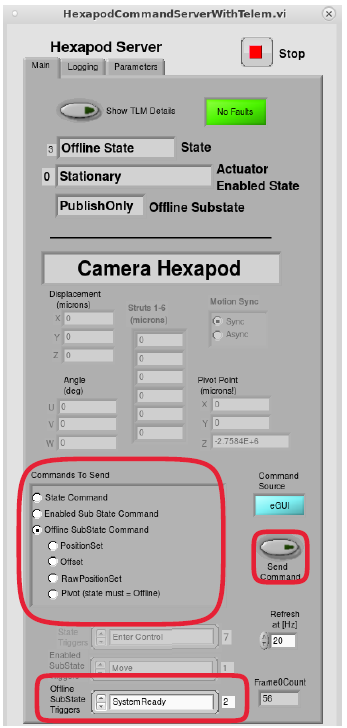
\includegraphics[width=1.79167in,height=\textheight]{jira_imgs/1024.png}

}
\hdashrule[0.5ex]{\textwidth}{1pt}{3mm}
  Expected Result \\
{\footnotesize
The system transitions from the OfflineState/PublishOnly substate to the
OfflineState/AvailableState substate and the Command Source says eGUI.\\
\strut \\

}
\hdashrule[0.5ex]{\textwidth}{1pt}{3mm}
  Actual Result \\
{\footnotesize
Successfully transitioned to the OfflineState/AvailableState substate.

}
\begin{tabular}{p{2cm}p{14cm}}
\toprule
Step 7 & Step Execution Status: \textbf{ Pass } \\ \hline
\end{tabular}
 Description \\
{\footnotesize
\textbf{Transition from OFFLINE State to STANDBY State.}

\hfill\break

On \textbf{Commands to Send}, select the \textbf{State Commands~}radio
button\textbf{.}

On \textbf{State Triggers}, scroll and select \textbf{Enter Control}.

Finally,\textbf{~}click on the \textbf{Send Command} button.

\hfill\break

The Hexapod should go to \textbf{STANDBY} state.

\hfill\break
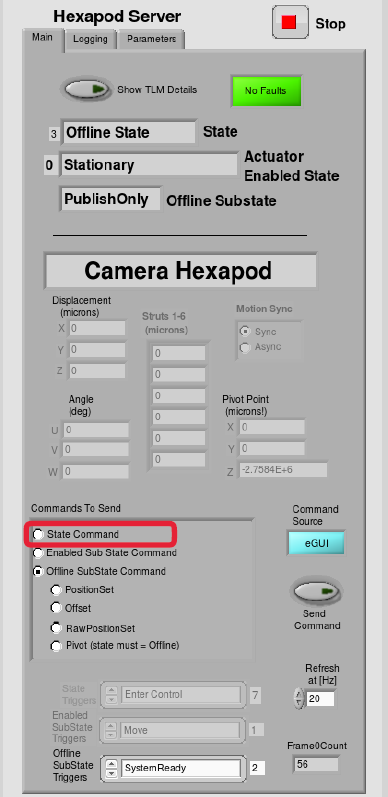
\includegraphics[width=1.79167in,height=\textheight]{jira_imgs/1028.png}

}
\hdashrule[0.5ex]{\textwidth}{1pt}{3mm}
  Expected Result \\
{\footnotesize
The system transitions to the Standby state and the primary state
display box at the top of the Main says Standby state.

}
\hdashrule[0.5ex]{\textwidth}{1pt}{3mm}
  Actual Result \\
{\footnotesize
The system transitioned successfully to the standbyState.

}
\begin{tabular}{p{2cm}p{14cm}}
\toprule
Step 8 & Step Execution Status: \textbf{ Pass } \\ \hline
\end{tabular}
 Description \\
{\footnotesize
\textbf{Transition from STANDBY State to DISABLED State.}

\hfill\break

On \textbf{Commands to Send}, select the \textbf{State Commands~}radio
button.

On \textbf{State Triggers}, scroll and select the \textbf{Start~}option.

Click on the \textbf{Send Command} button.

\hfill\break

The Hexapod should go to DISABLED state.

}
\hdashrule[0.5ex]{\textwidth}{1pt}{3mm}
  Expected Result \\
{\footnotesize
The system transitions into DISABLED State and the current configuration
parameters are maintained from the default parameters or from the
previous DDS start command.

}
\hdashrule[0.5ex]{\textwidth}{1pt}{3mm}
  Actual Result \\
{\footnotesize
The system transitioned successfully to the disabledState.

}
\begin{tabular}{p{2cm}p{14cm}}
\toprule
Step 9 & Step Execution Status: \textbf{ Pass } \\ \hline
\end{tabular}
 Description \\
{\footnotesize
\textbf{Transition from DISABLED State to ENABLED State.}

On \textbf{Commands to Send}, select the \textbf{State Commands~}radio
button.

On \textbf{State Triggers}, scroll and select the
\textbf{Enabled~}option.

Click on the \textbf{Send Command~}button.

The Hexapod should go to ENABLED state.

}
\hdashrule[0.5ex]{\textwidth}{1pt}{3mm}
  Expected Result \\
{\footnotesize
The system transitions into the ENABLED State/Stationary sub-state, the
motor drives are enabled and motion can be commanded.

}
\hdashrule[0.5ex]{\textwidth}{1pt}{3mm}
  Actual Result \\
{\footnotesize
The system transitioned successfully to the enabledState.

}
\begin{tabular}{p{2cm}p{14cm}}
\toprule
Step 10 & Step Execution Status: \textbf{ Not Executed } \\ \hline
\end{tabular}
 Description \\
{\footnotesize
\textless conditional state\textgreater{}\\
\strut \\
\textbf{Recovering from a FAULT State}\\
\strut \\
If a fault occurs in any of the other states, the system will
automatically transition to the FAULT State.\\
While in the Fault state, select the \textbf{clearError} option in the
\textbf{State Triggers~}option list. Then, click on the \textbf{Send
Command~}button\textbf{.}\\
\strut \\
\ul{Note:} If the fault that occurs goes through the interlock system,
reset the safety relay switch and send a \textbf{clearError} command.

}
\hdashrule[0.5ex]{\textwidth}{1pt}{3mm}
  Expected Result \\
{\footnotesize
The system transitions back to the STANDBY state. (Go back to Step 8)

}
\hdashrule[0.5ex]{\textwidth}{1pt}{3mm}
  Actual Result \\
{\footnotesize

}
\begin{tabular}{p{2cm}p{14cm}}
\toprule
Step 11 & Step Execution Status: \textbf{ Pass } \\ \hline
\end{tabular}
 Description \\
{\footnotesize
\textbf{Follow \emph{3.3.1 Positioning} of the LSST Hexapods-Rotator
Acceptance Test Procedure, Sheet 23-24.}

}
\hdashrule[0.5ex]{\textwidth}{1pt}{3mm}
  Test Data \\
 {\footnotesize
\textbf{Deviation:~}Depending on the configuration, this test is with no
performance payload or ComCam installed. The test is at a single
elevation angle of zero degrees. The tester monitors the temperature
using the EFD.

}
\hdashrule[0.5ex]{\textwidth}{1pt}{3mm}
  Expected Result \\
{\footnotesize
The position of the hexapod is able to be commanded, and no software
limits or limit switches are tripped.\\
The position of the hexapod is able to reach the commanded positions
within the absolute accuracy specifications of 25um in Z, 125um in XY,
205x10-5deg in RXRY, and 1500x10-5deg in RZ.

}
\hdashrule[0.5ex]{\textwidth}{1pt}{3mm}
  Actual Result \\
{\footnotesize
The test is successfully executed, considering the precision of the
laser tracker.\\
Details results are in cam.Hex.verif\_06072021\_30-31032022\_v4.xls\\

\begin{longtable}[]{@{}
  >{\centering\arraybackslash}p{(\columnwidth - 28\tabcolsep) * \real{0.0667}}
  >{\raggedright\arraybackslash}p{(\columnwidth - 28\tabcolsep) * \real{0.0667}}
  >{\centering\arraybackslash}p{(\columnwidth - 28\tabcolsep) * \real{0.0667}}
  >{\centering\arraybackslash}p{(\columnwidth - 28\tabcolsep) * \real{0.0667}}
  >{\centering\arraybackslash}p{(\columnwidth - 28\tabcolsep) * \real{0.0667}}
  >{\centering\arraybackslash}p{(\columnwidth - 28\tabcolsep) * \real{0.0667}}
  >{\centering\arraybackslash}p{(\columnwidth - 28\tabcolsep) * \real{0.0667}}
  >{\centering\arraybackslash}p{(\columnwidth - 28\tabcolsep) * \real{0.0667}}
  >{\centering\arraybackslash}p{(\columnwidth - 28\tabcolsep) * \real{0.0667}}
  >{\centering\arraybackslash}p{(\columnwidth - 28\tabcolsep) * \real{0.0667}}
  >{\raggedright\arraybackslash}p{(\columnwidth - 28\tabcolsep) * \real{0.0667}}
  >{\raggedright\arraybackslash}p{(\columnwidth - 28\tabcolsep) * \real{0.0667}}
  >{\centering\arraybackslash}p{(\columnwidth - 28\tabcolsep) * \real{0.0667}}
  >{\centering\arraybackslash}p{(\columnwidth - 28\tabcolsep) * \real{0.0667}}
  >{\raggedright\arraybackslash}p{(\columnwidth - 28\tabcolsep) * \real{0.0667}}@{}}
\toprule\noalign{}
\endhead
\bottomrule\noalign{}
\endlastfoot
10 & Hexapod Positioning (32 positions) ~ ~ ~ ~ ~ ~ ~ ~ ~ ~ ~ ~ ~ ~ ~ ~
~ ~ ~ ~ ~ ~ ~ ~ ~ ~ ~ {(LTS-206,~}{3.3.1}{)} & Trans & XY & Absolute &
~+/-7.6mm & \textless125um & Laser Tracker & \textless29um RMS & YES &
\begin{minipage}[t]{\linewidth}\raggedright
\hfill\break
\strut
\end{minipage} & \begin{minipage}[t]{\linewidth}\raggedright
\hfill\break
\strut
\end{minipage} & max. \textless119um & YES & ~stdev 36um \\
\begin{minipage}[t]{\linewidth}\centering
\hfill\break
\strut
\end{minipage} & \begin{minipage}[t]{\linewidth}\raggedright
\hfill\break
\strut
\end{minipage} & \begin{minipage}[t]{\linewidth}\centering
\hfill\break
\strut
\end{minipage} & Z & Absolute & ~+/-7.73mm & \textless25um & Laser
Tracker & \textless31um RMS & YES (Marginal) & L.T. resol. &
\begin{minipage}[t]{\linewidth}\raggedright
\hfill\break
\strut
\end{minipage} & max.\textless30um~ & YES (Marginal) & L.T.
res.\textasciitilde30um (3 outliers) \\
\begin{minipage}[t]{\linewidth}\centering
\hfill\break
\strut
\end{minipage} & \begin{minipage}[t]{\linewidth}\raggedright
\hfill\break
\strut
\end{minipage} & Rot & RxRy & Absolute & ~+/-0.17Deg &
\textless0.00205Deg & Laser Tracker & \textless0.0016Deg RMS & YES &
\begin{minipage}[t]{\linewidth}\raggedright
\hfill\break
\strut
\end{minipage} & \begin{minipage}[t]{\linewidth}\raggedright
\hfill\break
\strut
\end{minipage} & max.\textless0.0025{Deg} & YES (Marginal) & 6 outliers
(due to noise) \\
\begin{minipage}[t]{\linewidth}\centering
\hfill\break
\strut
\end{minipage} & \begin{minipage}[t]{\linewidth}\raggedright
\hfill\break
\strut
\end{minipage} & \begin{minipage}[t]{\linewidth}\centering
\hfill\break
\strut
\end{minipage} & Rz & Absolute & 0 & \textless0.015Deg & Laser Tracker &
Not checked & ~-\/-\/-\/-\/-\/- & tbd &
\begin{minipage}[t]{\linewidth}\raggedright
\hfill\break
\strut
\end{minipage} & max.\textless0.004{Deg} & YES &
\begin{minipage}[t]{\linewidth}\raggedright
\hfill\break
\strut
\end{minipage} \\
\end{longtable}

}
\begin{tabular}{p{2cm}p{14cm}}
\toprule
Step 12 & Step Execution Status: \textbf{ Pass } \\ \hline
\end{tabular}
 Description \\
{\footnotesize
\textbf{Follow \emph{3.3.2 Centers of Rotation} of the LSST
Hexapods-Rotator Acceptance Test Procedure, Sheet 24-25.}

}
\hdashrule[0.5ex]{\textwidth}{1pt}{3mm}
  Test Data \\
 {\footnotesize
\textbf{Deviation:~}Record pivot position through the EUI. The tester
monitors the temperature using the EFD.

}
\hdashrule[0.5ex]{\textwidth}{1pt}{3mm}
  Expected Result \\
{\footnotesize
The center of rotation is able to be moved.

}
\hdashrule[0.5ex]{\textwidth}{1pt}{3mm}
  Actual Result \\
{\footnotesize
The test is successfully executed, \textbf{considering the precision of
the laser tracker.}\\
Details results are in cam.Hex.verif\_06072021\_30-31032022\_v4.xls\\

\begin{longtable}[]{@{}
  >{\centering\arraybackslash}p{(\columnwidth - 28\tabcolsep) * \real{0.0667}}
  >{\raggedright\arraybackslash}p{(\columnwidth - 28\tabcolsep) * \real{0.0667}}
  >{\centering\arraybackslash}p{(\columnwidth - 28\tabcolsep) * \real{0.0667}}
  >{\raggedright\arraybackslash}p{(\columnwidth - 28\tabcolsep) * \real{0.0667}}
  >{\centering\arraybackslash}p{(\columnwidth - 28\tabcolsep) * \real{0.0667}}
  >{\raggedright\arraybackslash}p{(\columnwidth - 28\tabcolsep) * \real{0.0667}}
  >{\raggedright\arraybackslash}p{(\columnwidth - 28\tabcolsep) * \real{0.0667}}
  >{\raggedright\arraybackslash}p{(\columnwidth - 28\tabcolsep) * \real{0.0667}}
  >{\raggedright\arraybackslash}p{(\columnwidth - 28\tabcolsep) * \real{0.0667}}
  >{\raggedright\arraybackslash}p{(\columnwidth - 28\tabcolsep) * \real{0.0667}}
  >{\raggedright\arraybackslash}p{(\columnwidth - 28\tabcolsep) * \real{0.0667}}
  >{\raggedright\arraybackslash}p{(\columnwidth - 28\tabcolsep) * \real{0.0667}}
  >{\raggedright\arraybackslash}p{(\columnwidth - 28\tabcolsep) * \real{0.0667}}
  >{\raggedright\arraybackslash}p{(\columnwidth - 28\tabcolsep) * \real{0.0667}}
  >{\raggedright\arraybackslash}p{(\columnwidth - 28\tabcolsep) * \real{0.0667}}@{}}
\toprule\noalign{}
\endhead
\bottomrule\noalign{}
\endlastfoot
\begin{minipage}[t]{\linewidth}\centering
\hfill\break
\strut
\end{minipage} & \begin{minipage}[t]{\linewidth}\raggedright
\hfill\break
\strut
\end{minipage} & \begin{minipage}[t]{\linewidth}\centering
\hfill\break
\strut
\end{minipage} & \begin{minipage}[t]{\linewidth}\raggedright
\hfill\break
\strut
\end{minipage} & \begin{minipage}[t]{\linewidth}\centering
\hfill\break
\strut
\end{minipage} & \begin{minipage}[t]{\linewidth}\raggedright
\hfill\break
\strut
\end{minipage} & \begin{minipage}[t]{\linewidth}\raggedright
\hfill\break
\strut
\end{minipage} & \begin{minipage}[t]{\linewidth}\raggedright
\hfill\break
\strut
\end{minipage} & \multicolumn{3}{l}{%
Camera Hexapod Re-verification 2021} &
\begin{minipage}[t]{\linewidth}\raggedright
\hfill\break
\strut
\end{minipage} & \multicolumn{3}{l@{}}{%
Camera Hexapod Re-verification 2022} \\
\begin{minipage}[t]{\linewidth}\centering
\hfill\break
\strut
\end{minipage} & \begin{minipage}[t]{\linewidth}\raggedright
\hfill\break
\strut
\end{minipage} & \begin{minipage}[t]{\linewidth}\centering
\hfill\break
\strut
\end{minipage} & \begin{minipage}[t]{\linewidth}\raggedright
\hfill\break
\strut
\end{minipage} & \begin{minipage}[t]{\linewidth}\centering
\hfill\break
\strut
\end{minipage} & \begin{minipage}[t]{\linewidth}\raggedright
\hfill\break
\strut
\end{minipage} & \begin{minipage}[t]{\linewidth}\raggedright
\hfill\break
\strut
\end{minipage} & \begin{minipage}[t]{\linewidth}\raggedright
\hfill\break
\strut
\end{minipage} & \multicolumn{3}{l}{%
(no load on Hexapod\&Rotator unit)} &
\begin{minipage}[t]{\linewidth}\raggedright
\hfill\break
\strut
\end{minipage} & \multicolumn{3}{l@{}}{%
(with ComCam mounted on Rotator\&Hexapod)} \\
\multicolumn{8}{@{}c}{%
~ LSST Camera Hexapod Requirement specifications re-verification.
Ordered from tighter to looser specs, based on document LTS-206,
{[}1{]}} & \begin{minipage}[t]{\linewidth}\raggedright
\hfill\break
\strut
\end{minipage} & \begin{minipage}[t]{\linewidth}\raggedright
\hfill\break
\strut
\end{minipage} & \begin{minipage}[t]{\linewidth}\raggedright
\hfill\break
\strut
\end{minipage} & \begin{minipage}[t]{\linewidth}\raggedright
\hfill\break
\strut
\end{minipage} & \multicolumn{3}{l@{}}{%
{~February-March 2022}{~w/ComCom on Rotator}} \\
Specs & ITEM & MOVE & AXIS & MODE & SPEC & ERROR SPEC & MEASUREMENT &
MEASURED & MEET SPEC & Notes \& &
\begin{minipage}[t]{\linewidth}\centering
\hfill\break
\strut
\end{minipage} & MEASURED & MEET SPEC & Notes \& \\
Index & \begin{minipage}[t]{\linewidth}\raggedright
\hfill\break
\strut
\end{minipage} & \begin{minipage}[t]{\linewidth}\centering
\hfill\break
\strut
\end{minipage} & \begin{minipage}[t]{\linewidth}\centering
\hfill\break
\strut
\end{minipage} & \begin{minipage}[t]{\linewidth}\centering
\hfill\break
\strut
\end{minipage} & (LTS-206) & \begin{minipage}[t]{\linewidth}\centering
\hfill\break
\strut
\end{minipage} & Instrument & ERROR &
\begin{minipage}[t]{\linewidth}\centering
\hfill\break
\strut
\end{minipage} & Comments & \begin{minipage}[t]{\linewidth}\centering
\hfill\break
\strut
\end{minipage} & ERROR & \begin{minipage}[t]{\linewidth}\centering
\hfill\break
\strut
\end{minipage} & Comments \\
\end{longtable}

\hfill\break

\begin{longtable}[]{@{}
  >{\centering\arraybackslash}p{(\columnwidth - 28\tabcolsep) * \real{0.0667}}
  >{\raggedright\arraybackslash}p{(\columnwidth - 28\tabcolsep) * \real{0.0667}}
  >{\centering\arraybackslash}p{(\columnwidth - 28\tabcolsep) * \real{0.0667}}
  >{\centering\arraybackslash}p{(\columnwidth - 28\tabcolsep) * \real{0.0667}}
  >{\centering\arraybackslash}p{(\columnwidth - 28\tabcolsep) * \real{0.0667}}
  >{\centering\arraybackslash}p{(\columnwidth - 28\tabcolsep) * \real{0.0667}}
  >{\raggedright\arraybackslash}p{(\columnwidth - 28\tabcolsep) * \real{0.0667}}
  >{\raggedright\arraybackslash}p{(\columnwidth - 28\tabcolsep) * \real{0.0667}}
  >{\raggedright\arraybackslash}p{(\columnwidth - 28\tabcolsep) * \real{0.0667}}
  >{\raggedright\arraybackslash}p{(\columnwidth - 28\tabcolsep) * \real{0.0667}}
  >{\raggedright\arraybackslash}p{(\columnwidth - 28\tabcolsep) * \real{0.0667}}
  >{\raggedright\arraybackslash}p{(\columnwidth - 28\tabcolsep) * \real{0.0667}}
  >{\raggedright\arraybackslash}p{(\columnwidth - 28\tabcolsep) * \real{0.0667}}
  >{\raggedright\arraybackslash}p{(\columnwidth - 28\tabcolsep) * \real{0.0667}}
  >{\raggedright\arraybackslash}p{(\columnwidth - 28\tabcolsep) * \real{0.0667}}@{}}
\toprule\noalign{}
\endhead
\bottomrule\noalign{}
\endlastfoot
11 & Hexapod centers of rotation{~ ~ ~ ~ ~ ~ ~ ~ ~ ~ ~ ~ ~ ~ ~ ~ ~ ~ ~ ~
~ ~ ~ ~ ~ ~ ~ ~ ~ ~ ~ ~ ~ (LTS-206,~}{3.3.2}{)} & Rot \& & Rx & Absolute
& 0.04 to 0.24 Deg & \begin{minipage}[t]{\linewidth}\raggedright
\hfill\break
\strut
\end{minipage} & \begin{minipage}[t]{\linewidth}\raggedright
\hfill\break
\strut
\end{minipage} & \begin{minipage}[t]{\linewidth}\raggedright
\hfill\break
\strut
\end{minipage} & \begin{minipage}[t]{\linewidth}\raggedright
\hfill\break
\strut
\end{minipage} & \begin{minipage}[t]{\linewidth}\raggedright
\hfill\break
\strut
\end{minipage} & \begin{minipage}[t]{\linewidth}\raggedright
\hfill\break
\strut
\end{minipage} & \begin{minipage}[t]{\linewidth}\raggedright
\hfill\break
\strut
\end{minipage} & \begin{minipage}[t]{\linewidth}\raggedright
\hfill\break
\strut
\end{minipage} & \begin{minipage}[t]{\linewidth}\raggedright
\hfill\break
\strut
\end{minipage} \\
\begin{minipage}[t]{\linewidth}\centering
\hfill\break
\strut
\end{minipage} & (Y offset measured-expected, due to Rx rotation for a
given COR, should be \textless125um) & Trans & Y &
\begin{minipage}[t]{\linewidth}\centering
\hfill\break
\strut
\end{minipage} & Y=pivot*Rx & {ΔY}{\textless125um} & Laser Tracker &
\textless35um RMS & YES & \begin{minipage}[t]{\linewidth}\raggedright
\hfill\break
\strut
\end{minipage} & \begin{minipage}[t]{\linewidth}\raggedright
\hfill\break
\strut
\end{minipage} & max.\textless19um & YES &
\begin{minipage}[t]{\linewidth}\raggedright
\hfill\break
\strut
\end{minipage} \\
\end{longtable}

}
\begin{tabular}{p{2cm}p{14cm}}
\toprule
Step 13 & Step Execution Status: \textbf{ Pass } \\ \hline
\end{tabular}
 Description \\
{\footnotesize
\textbf{Follow \emph{3.3.3 Cross-Talk Motion~}of the LSST
Hexapods-Rotator Acceptance Test Procedure, Sheet 25.}

}
\hdashrule[0.5ex]{\textwidth}{1pt}{3mm}
  Expected Result \\
{\footnotesize
There is no cross-talk observed (actuator positioning errors and
erroneous geometry are minimal).

}
\hdashrule[0.5ex]{\textwidth}{1pt}{3mm}
  Actual Result \\
{\footnotesize
The test is successfully executed, considering the precision of the
laser tracker.\\
Details results are in cam.Hex.verif\_06072021\_30-31032022\_v4.xls\\

\begin{longtable}[]{@{}
  >{\centering\arraybackslash}p{(\columnwidth - 28\tabcolsep) * \real{0.0667}}
  >{\raggedright\arraybackslash}p{(\columnwidth - 28\tabcolsep) * \real{0.0667}}
  >{\centering\arraybackslash}p{(\columnwidth - 28\tabcolsep) * \real{0.0667}}
  >{\raggedright\arraybackslash}p{(\columnwidth - 28\tabcolsep) * \real{0.0667}}
  >{\centering\arraybackslash}p{(\columnwidth - 28\tabcolsep) * \real{0.0667}}
  >{\raggedright\arraybackslash}p{(\columnwidth - 28\tabcolsep) * \real{0.0667}}
  >{\raggedright\arraybackslash}p{(\columnwidth - 28\tabcolsep) * \real{0.0667}}
  >{\raggedright\arraybackslash}p{(\columnwidth - 28\tabcolsep) * \real{0.0667}}
  >{\raggedright\arraybackslash}p{(\columnwidth - 28\tabcolsep) * \real{0.0667}}
  >{\raggedright\arraybackslash}p{(\columnwidth - 28\tabcolsep) * \real{0.0667}}
  >{\raggedright\arraybackslash}p{(\columnwidth - 28\tabcolsep) * \real{0.0667}}
  >{\raggedright\arraybackslash}p{(\columnwidth - 28\tabcolsep) * \real{0.0667}}
  >{\raggedright\arraybackslash}p{(\columnwidth - 28\tabcolsep) * \real{0.0667}}
  >{\raggedright\arraybackslash}p{(\columnwidth - 28\tabcolsep) * \real{0.0667}}
  >{\raggedright\arraybackslash}p{(\columnwidth - 28\tabcolsep) * \real{0.0667}}@{}}
\toprule\noalign{}
\endhead
\bottomrule\noalign{}
\endlastfoot
\begin{minipage}[t]{\linewidth}\centering
\hfill\break
\strut
\end{minipage} & \begin{minipage}[t]{\linewidth}\raggedright
\hfill\break
\strut
\end{minipage} & \begin{minipage}[t]{\linewidth}\centering
\hfill\break
\strut
\end{minipage} & \begin{minipage}[t]{\linewidth}\raggedright
\hfill\break
\strut
\end{minipage} & \begin{minipage}[t]{\linewidth}\centering
\hfill\break
\strut
\end{minipage} & \begin{minipage}[t]{\linewidth}\raggedright
\hfill\break
\strut
\end{minipage} & \begin{minipage}[t]{\linewidth}\raggedright
\hfill\break
\strut
\end{minipage} & \begin{minipage}[t]{\linewidth}\raggedright
\hfill\break
\strut
\end{minipage} & \multicolumn{3}{l}{%
Camera Hexapod Re-verification 2021} &
\begin{minipage}[t]{\linewidth}\raggedright
\hfill\break
\strut
\end{minipage} & \multicolumn{3}{l@{}}{%
Camera Hexapod Re-verification 2022} \\
\begin{minipage}[t]{\linewidth}\centering
\hfill\break
\strut
\end{minipage} & \begin{minipage}[t]{\linewidth}\raggedright
\hfill\break
\strut
\end{minipage} & \begin{minipage}[t]{\linewidth}\centering
\hfill\break
\strut
\end{minipage} & \begin{minipage}[t]{\linewidth}\raggedright
\hfill\break
\strut
\end{minipage} & \begin{minipage}[t]{\linewidth}\centering
\hfill\break
\strut
\end{minipage} & \begin{minipage}[t]{\linewidth}\raggedright
\hfill\break
\strut
\end{minipage} & \begin{minipage}[t]{\linewidth}\raggedright
\hfill\break
\strut
\end{minipage} & \begin{minipage}[t]{\linewidth}\raggedright
\hfill\break
\strut
\end{minipage} & \multicolumn{3}{l}{%
(no load on Hexapod\&Rotator unit)} &
\begin{minipage}[t]{\linewidth}\raggedright
\hfill\break
\strut
\end{minipage} & \multicolumn{3}{l@{}}{%
(with ComCam mounted on Rotator\&Hexapod)} \\
\multicolumn{8}{@{}c}{%
~ LSST Camera Hexapod Requirement specifications re-verification.
Ordered from tighter to looser specs, based on document LTS-206,
{[}1{]}} & \begin{minipage}[t]{\linewidth}\raggedright
\hfill\break
\strut
\end{minipage} & \begin{minipage}[t]{\linewidth}\raggedright
\hfill\break
\strut
\end{minipage} & \begin{minipage}[t]{\linewidth}\raggedright
\hfill\break
\strut
\end{minipage} & \begin{minipage}[t]{\linewidth}\raggedright
\hfill\break
\strut
\end{minipage} & \multicolumn{3}{l@{}}{%
{~February-March 2022}{~w/ComCom on Rotator}} \\
Specs & ITEM & MOVE & AXIS & MODE & SPEC & ERROR SPEC & MEASUREMENT &
MEASURED & MEET SPEC & Notes \& &
\begin{minipage}[t]{\linewidth}\centering
\hfill\break
\strut
\end{minipage} & MEASURED & MEET SPEC & Notes \& \\
Index & \begin{minipage}[t]{\linewidth}\raggedright
\hfill\break
\strut
\end{minipage} & \begin{minipage}[t]{\linewidth}\centering
\hfill\break
\strut
\end{minipage} & \begin{minipage}[t]{\linewidth}\centering
\hfill\break
\strut
\end{minipage} & \begin{minipage}[t]{\linewidth}\centering
\hfill\break
\strut
\end{minipage} & (LTS-206) & \begin{minipage}[t]{\linewidth}\centering
\hfill\break
\strut
\end{minipage} & Instrument & ERROR &
\begin{minipage}[t]{\linewidth}\centering
\hfill\break
\strut
\end{minipage} & Comments & \begin{minipage}[t]{\linewidth}\centering
\hfill\break
\strut
\end{minipage} & ERROR & \begin{minipage}[t]{\linewidth}\centering
\hfill\break
\strut
\end{minipage} & Comments \\
\end{longtable}

~

\begin{longtable}[]{@{}
  >{\centering\arraybackslash}p{(\columnwidth - 28\tabcolsep) * \real{0.0667}}
  >{\raggedright\arraybackslash}p{(\columnwidth - 28\tabcolsep) * \real{0.0667}}
  >{\centering\arraybackslash}p{(\columnwidth - 28\tabcolsep) * \real{0.0667}}
  >{\centering\arraybackslash}p{(\columnwidth - 28\tabcolsep) * \real{0.0667}}
  >{\centering\arraybackslash}p{(\columnwidth - 28\tabcolsep) * \real{0.0667}}
  >{\centering\arraybackslash}p{(\columnwidth - 28\tabcolsep) * \real{0.0667}}
  >{\centering\arraybackslash}p{(\columnwidth - 28\tabcolsep) * \real{0.0667}}
  >{\centering\arraybackslash}p{(\columnwidth - 28\tabcolsep) * \real{0.0667}}
  >{\centering\arraybackslash}p{(\columnwidth - 28\tabcolsep) * \real{0.0667}}
  >{\centering\arraybackslash}p{(\columnwidth - 28\tabcolsep) * \real{0.0667}}
  >{\raggedright\arraybackslash}p{(\columnwidth - 28\tabcolsep) * \real{0.0667}}
  >{\raggedright\arraybackslash}p{(\columnwidth - 28\tabcolsep) * \real{0.0667}}
  >{\centering\arraybackslash}p{(\columnwidth - 28\tabcolsep) * \real{0.0667}}
  >{\centering\arraybackslash}p{(\columnwidth - 28\tabcolsep) * \real{0.0667}}
  >{\raggedright\arraybackslash}p{(\columnwidth - 28\tabcolsep) * \real{0.0667}}@{}}
\toprule\noalign{}
\endhead
\bottomrule\noalign{}
\endlastfoot
12 & Hexapod cross-talk motion ~ ~ ~ ~ ~ ~ ~ ~ ~ ~ ~ ~ ~ ~ ~ ~ ~ ~ ~ ~ ~
~ ~ ~ ~ ~ ~ ~ ~ ~ ~ ~ ~ {(LTS-206,~}{3.3.3}{)} & Trans & X & Absolute &
~0mm & \textless125um & Laser Tracker & \textless30um & YES &
\begin{minipage}[t]{\linewidth}\raggedright
\hfill\break
\strut
\end{minipage} & \begin{minipage}[t]{\linewidth}\raggedright
\hfill\break
\strut
\end{minipage} & \textless{} 50um & YES &
\begin{minipage}[t]{\linewidth}\raggedright
\hfill\break
\strut
\end{minipage} \\
\begin{minipage}[t]{\linewidth}\centering
\hfill\break
\strut
\end{minipage} & (moves should be reached with inactive axes residuals X
and Y\textless125um and Z\textless25um) &
\begin{minipage}[t]{\linewidth}\centering
\hfill\break
\strut
\end{minipage} & Y & Absolute & ~0mm & \textless125um & Laser Tracker &
\textless50um & YES & \begin{minipage}[t]{\linewidth}\raggedright
\hfill\break
\strut
\end{minipage} & \begin{minipage}[t]{\linewidth}\raggedright
\hfill\break
\strut
\end{minipage} & \textless{} 17um & YES &
\begin{minipage}[t]{\linewidth}\raggedright
\hfill\break
\strut
\end{minipage} \\
\begin{minipage}[t]{\linewidth}\centering
\hfill\break
\strut
\end{minipage} & (data from the measurements of 3.3.4 and 3.3.8 above) &
\begin{minipage}[t]{\linewidth}\centering
\hfill\break
\strut
\end{minipage} & Z & Absolute & ~0mm & \textless25um & Laser Tracker &
\textless27um RMS & YES & \begin{minipage}[t]{\linewidth}\raggedright
\hfill\break
\strut
\end{minipage} & \begin{minipage}[t]{\linewidth}\raggedright
\hfill\break
\strut
\end{minipage} & \textless{} 13um & YES &
\begin{minipage}[t]{\linewidth}\raggedright
\hfill\break
\strut
\end{minipage} \\
\begin{minipage}[t]{\linewidth}\centering
\hfill\break
\strut
\end{minipage} & \begin{minipage}[t]{\linewidth}\raggedright
\hfill\break
\strut
\end{minipage} & \begin{minipage}[t]{\linewidth}\centering
\hfill\break
\strut
\end{minipage} & Rx & Absolute & 0Deg & \textless0.00205Deg & Laser
Tracker & Not checked & ~-\/-\/-\/-\/-\/- &
\begin{minipage}[t]{\linewidth}\raggedright
\hfill\break
\strut
\end{minipage} & \begin{minipage}[t]{\linewidth}\raggedright
\hfill\break
\strut
\end{minipage} & max.\textless0.0037Deg & Yes (marginal) & Stdev
=0.0020Deg \\
\begin{minipage}[t]{\linewidth}\centering
\hfill\break
\strut
\end{minipage} & \begin{minipage}[t]{\linewidth}\raggedright
\hfill\break
\strut
\end{minipage} & \begin{minipage}[t]{\linewidth}\centering
\hfill\break
\strut
\end{minipage} & Ry & Absolute & 0Deg & \textless0.00205Deg & Laser
Tracker & Not checked & ~-\/-\/-\/-\/-\/- &
\begin{minipage}[t]{\linewidth}\raggedright
\hfill\break
\strut
\end{minipage} & \begin{minipage}[t]{\linewidth}\raggedright
\hfill\break
\strut
\end{minipage} & \textless0.0017Deg & YES &
\begin{minipage}[t]{\linewidth}\raggedright
\hfill\break
\strut
\end{minipage} \\
\begin{minipage}[t]{\linewidth}\centering
\hfill\break
\strut
\end{minipage} & \begin{minipage}[t]{\linewidth}\raggedright
\hfill\break
\strut
\end{minipage} & \begin{minipage}[t]{\linewidth}\centering
\hfill\break
\strut
\end{minipage} & Rz & Absolute & 0Deg & \textless0.015Deg & Laser
Tracker & Not checked & ~-\/-\/-\/-\/-\/- &
\begin{minipage}[t]{\linewidth}\raggedright
\hfill\break
\strut
\end{minipage} & \begin{minipage}[t]{\linewidth}\raggedright
\hfill\break
\strut
\end{minipage} & \textless0.0049Deg & YES &
\begin{minipage}[t]{\linewidth}\raggedright
\hfill\break
\strut
\end{minipage} \\
\end{longtable}

\hfill\break
Detailed test data:\\
\strut \\

\begin{longtable}[]{@{}
  >{\raggedright\arraybackslash}p{(\columnwidth - 18\tabcolsep) * \real{0.1000}}
  >{\centering\arraybackslash}p{(\columnwidth - 18\tabcolsep) * \real{0.1000}}
  >{\centering\arraybackslash}p{(\columnwidth - 18\tabcolsep) * \real{0.1000}}
  >{\centering\arraybackslash}p{(\columnwidth - 18\tabcolsep) * \real{0.1000}}
  >{\centering\arraybackslash}p{(\columnwidth - 18\tabcolsep) * \real{0.1000}}
  >{\centering\arraybackslash}p{(\columnwidth - 18\tabcolsep) * \real{0.1000}}
  >{\centering\arraybackslash}p{(\columnwidth - 18\tabcolsep) * \real{0.1000}}
  >{\centering\arraybackslash}p{(\columnwidth - 18\tabcolsep) * \real{0.1000}}
  >{\centering\arraybackslash}p{(\columnwidth - 18\tabcolsep) * \real{0.1000}}
  >{\centering\arraybackslash}p{(\columnwidth - 18\tabcolsep) * \real{0.1000}}@{}}
\toprule\noalign{}
\endhead
\bottomrule\noalign{}
\endlastfoot
\begin{minipage}[t]{\linewidth}\raggedright
\hfill\break
\strut
\end{minipage} & \multicolumn{9}{c@{}}{%
\multirow{2}{*}{absolute accuracy cross-talk}} \\
\begin{minipage}[t]{\linewidth}\raggedright
\hfill\break
\strut
\end{minipage} \\
\begin{minipage}[t]{\linewidth}\raggedright
\hfill\break
\strut
\end{minipage} & \begin{minipage}[t]{\linewidth}\centering
\hfill\break
\strut
\end{minipage} & 24/03/2022 & \begin{minipage}[t]{\linewidth}\centering
\hfill\break
\strut
\end{minipage} & \multicolumn{4}{c}{%
(data from the measurements of 3.3.4 and 3.3.8)} &
\begin{minipage}[t]{\linewidth}\centering
\hfill\break
\strut
\end{minipage} & \begin{minipage}[t]{\linewidth}\centering
\hfill\break
\strut
\end{minipage} \\
\begin{minipage}[t]{\linewidth}\raggedright
\hfill\break
\strut
\end{minipage} & X & Y & Z & \begin{minipage}[t]{\linewidth}\centering
\hfill\break
\strut
\end{minipage} & Rx & \begin{minipage}[t]{\linewidth}\centering
\hfill\break
\strut
\end{minipage} & Ry & \begin{minipage}[t]{\linewidth}\centering
\hfill\break
\strut
\end{minipage} & Rz \\
\begin{minipage}[t]{\linewidth}\raggedright
\hfill\break
\strut
\end{minipage} & 0,009 & -0,013 & -0,003 & 0,0002 & 0,0005 & 0,0016 &
0,0013 & -0,0043 & -0,0031 \\
\begin{minipage}[t]{\linewidth}\raggedright
\hfill\break
\strut
\end{minipage} & 0,050 & -0,008 & 0,010 & 0,0001 & 0,0004 & 0,0011 &
0,0008 & -0,0015 & -0,0003 \\
\begin{minipage}[t]{\linewidth}\raggedright
\hfill\break
\strut
\end{minipage} & 0,004 & -0,017 & -0,013 & -0,0013 & -0,0010 & 0,0001 &
-0,0002 & -0,0061 & -0,0049 \\
\begin{minipage}[t]{\linewidth}\raggedright
\hfill\break
\strut
\end{minipage} & 0,040 & -0,011 & 0,005 & -0,0007 & -0,0004 & -0,0001 &
-0,0004 & -0,0029 & -0,0017 \\
\begin{minipage}[t]{\linewidth}\raggedright
\hfill\break
\strut
\end{minipage} & 0,024 & -0,007 & -0,004 & -0,0001 & 0,0002 & 0,0009 &
0,0006 & -0,0001 & 0,0011 \\
\begin{minipage}[t]{\linewidth}\raggedright
\hfill\break
\strut
\end{minipage} & 0,042 & -0,014 & 0,011 & -0,0003 & 0,0000 & 0,0008 &
0,0005 & -0,0005 & 0,0007 \\
\begin{minipage}[t]{\linewidth}\raggedright
\hfill\break
\strut
\end{minipage} & 0,004 & -0,017 & 0,003 & -0,0012 & -0,0009 & 0,0008 &
0,0005 & -0,0036 & -0,0024 \\
\begin{minipage}[t]{\linewidth}\raggedright
\hfill\break
\strut
\end{minipage} & 0,035 & -0,006 & 0,007 & 0,0000 & 0,0003 & 0,0011 &
0,0008 & -0,0013 & -0,0001 \\
\begin{minipage}[t]{\linewidth}\raggedright
\hfill\break
\strut
\end{minipage} & 0,011 & -0,016 & 0,001 & -0,0026 & -0,0023 & -0,0010 &
-0,0013 & 0,0002 & 0,0014 \\
\begin{minipage}[t]{\linewidth}\raggedright
\hfill\break
\strut
\end{minipage} & \begin{minipage}[t]{\linewidth}\centering
\hfill\break
\strut
\end{minipage} & \begin{minipage}[t]{\linewidth}\centering
\hfill\break
\strut
\end{minipage} & \begin{minipage}[t]{\linewidth}\centering
\hfill\break
\strut
\end{minipage} & -0,0040 & -0,0037 & -0,0014 & -0,0017 & 0,0022 &
0,0034 \\
\begin{minipage}[t]{\linewidth}\raggedright
\hfill\break
\strut
\end{minipage} & \begin{minipage}[t]{\linewidth}\centering
\hfill\break
\strut
\end{minipage} & \begin{minipage}[t]{\linewidth}\centering
\hfill\break
\strut
\end{minipage} & \begin{minipage}[t]{\linewidth}\centering
\hfill\break
\strut
\end{minipage} & -0,0033 & -0,0030 & -0,0014 & -0,0017 & -0,0011 &
0,0001 \\
\begin{minipage}[t]{\linewidth}\raggedright
\hfill\break
\strut
\end{minipage} & \begin{minipage}[t]{\linewidth}\centering
\hfill\break
\strut
\end{minipage} & \begin{minipage}[t]{\linewidth}\centering
\hfill\break
\strut
\end{minipage} & \begin{minipage}[t]{\linewidth}\centering
\hfill\break
\strut
\end{minipage} & 0,0022 & 0,0025 & 0,0009 & 0,0006 & 0,0003 & 0,0015 \\
\begin{minipage}[t]{\linewidth}\raggedright
\hfill\break
\strut
\end{minipage} & \begin{minipage}[t]{\linewidth}\centering
\hfill\break
\strut
\end{minipage} & \begin{minipage}[t]{\linewidth}\centering
\hfill\break
\strut
\end{minipage} & \begin{minipage}[t]{\linewidth}\centering
\hfill\break
\strut
\end{minipage} & 0,0014 & 0,0017 & 0,0007 & 0,0004 & -0,0008 & 0,0004 \\
\begin{minipage}[t]{\linewidth}\raggedright
\hfill\break
\strut
\end{minipage} & \begin{minipage}[t]{\linewidth}\centering
\hfill\break
\strut
\end{minipage} & \begin{minipage}[t]{\linewidth}\centering
\hfill\break
\strut
\end{minipage} & \begin{minipage}[t]{\linewidth}\centering
\hfill\break
\strut
\end{minipage} & 0,0021 & 0,0024 & 0,0004 & 0,0001 & -0,0010 & 0,0002 \\
\begin{minipage}[t]{\linewidth}\raggedright
\hfill\break
\strut
\end{minipage} & \begin{minipage}[t]{\linewidth}\centering
\hfill\break
\strut
\end{minipage} & \begin{minipage}[t]{\linewidth}\centering
\hfill\break
\strut
\end{minipage} & \begin{minipage}[t]{\linewidth}\centering
\hfill\break
\strut
\end{minipage} & 0,0027 & 0,0030 &
\begin{minipage}[t]{\linewidth}\centering
\hfill\break
\strut
\end{minipage} & \begin{minipage}[t]{\linewidth}\centering
\hfill\break
\strut
\end{minipage} & -0,0022 & -0,0010 \\
\begin{minipage}[t]{\linewidth}\raggedright
\hfill\break
\strut
\end{minipage} & \begin{minipage}[t]{\linewidth}\centering
\hfill\break
\strut
\end{minipage} & \begin{minipage}[t]{\linewidth}\centering
\hfill\break
\strut
\end{minipage} & \begin{minipage}[t]{\linewidth}\centering
\hfill\break
\strut
\end{minipage} & \begin{minipage}[t]{\linewidth}\centering
\hfill\break
\strut
\end{minipage} & \begin{minipage}[t]{\linewidth}\centering
\hfill\break
\strut
\end{minipage} & \begin{minipage}[t]{\linewidth}\centering
\hfill\break
\strut
\end{minipage} & \begin{minipage}[t]{\linewidth}\centering
\hfill\break
\strut
\end{minipage} & 0,0029 & 0,0041 \\
\begin{minipage}[t]{\linewidth}\raggedright
\hfill\break
\strut
\end{minipage} & \begin{minipage}[t]{\linewidth}\centering
\hfill\break
\strut
\end{minipage} & \begin{minipage}[t]{\linewidth}\centering
\hfill\break
\strut
\end{minipage} & \begin{minipage}[t]{\linewidth}\centering
\hfill\break
\strut
\end{minipage} & \begin{minipage}[t]{\linewidth}\centering
\hfill\break
\strut
\end{minipage} & \begin{minipage}[t]{\linewidth}\centering
\hfill\break
\strut
\end{minipage} & \begin{minipage}[t]{\linewidth}\centering
\hfill\break
\strut
\end{minipage} & \begin{minipage}[t]{\linewidth}\centering
\hfill\break
\strut
\end{minipage} & -0,0011 & 0,0001 \\
\begin{minipage}[t]{\linewidth}\raggedright
\hfill\break
\strut
\end{minipage} & \begin{minipage}[t]{\linewidth}\centering
\hfill\break
\strut
\end{minipage} & \begin{minipage}[t]{\linewidth}\centering
\hfill\break
\strut
\end{minipage} & \begin{minipage}[t]{\linewidth}\centering
\hfill\break
\strut
\end{minipage} & \begin{minipage}[t]{\linewidth}\centering
\hfill\break
\strut
\end{minipage} & \begin{minipage}[t]{\linewidth}\centering
\hfill\break
\strut
\end{minipage} & \begin{minipage}[t]{\linewidth}\centering
\hfill\break
\strut
\end{minipage} & \begin{minipage}[t]{\linewidth}\centering
\hfill\break
\strut
\end{minipage} & -0,0001 & 0,0011 \\
\begin{minipage}[t]{\linewidth}\raggedright
\hfill\break
\strut
\end{minipage} & \begin{minipage}[t]{\linewidth}\centering
\hfill\break
\strut
\end{minipage} & \begin{minipage}[t]{\linewidth}\centering
\hfill\break
\strut
\end{minipage} & \begin{minipage}[t]{\linewidth}\centering
\hfill\break
\strut
\end{minipage} & \begin{minipage}[t]{\linewidth}\centering
\hfill\break
\strut
\end{minipage} & \begin{minipage}[t]{\linewidth}\centering
\hfill\break
\strut
\end{minipage} & \begin{minipage}[t]{\linewidth}\centering
\hfill\break
\strut
\end{minipage} & \begin{minipage}[t]{\linewidth}\centering
\hfill\break
\strut
\end{minipage} & -0,0003 & 0,0009 \\
\begin{minipage}[t]{\linewidth}\raggedright
\hfill\break
\strut
\end{minipage} & \begin{minipage}[t]{\linewidth}\centering
\hfill\break
\strut
\end{minipage} & \begin{minipage}[t]{\linewidth}\centering
\hfill\break
\strut
\end{minipage} & \begin{minipage}[t]{\linewidth}\centering
\hfill\break
\strut
\end{minipage} & \begin{minipage}[t]{\linewidth}\centering
\hfill\break
\strut
\end{minipage} & \begin{minipage}[t]{\linewidth}\centering
\hfill\break
\strut
\end{minipage} & \begin{minipage}[t]{\linewidth}\centering
\hfill\break
\strut
\end{minipage} & \begin{minipage}[t]{\linewidth}\centering
\hfill\break
\strut
\end{minipage} & -0,0018 & -0,0006 \\
\begin{minipage}[t]{\linewidth}\raggedright
\hfill\break
\strut
\end{minipage} & \begin{minipage}[t]{\linewidth}\centering
\hfill\break
\strut
\end{minipage} & \begin{minipage}[t]{\linewidth}\centering
\hfill\break
\strut
\end{minipage} & \begin{minipage}[t]{\linewidth}\centering
\hfill\break
\strut
\end{minipage} & \begin{minipage}[t]{\linewidth}\centering
\hfill\break
\strut
\end{minipage} & \begin{minipage}[t]{\linewidth}\centering
\hfill\break
\strut
\end{minipage} & \begin{minipage}[t]{\linewidth}\centering
\hfill\break
\strut
\end{minipage} & \begin{minipage}[t]{\linewidth}\centering
\hfill\break
\strut
\end{minipage} & -0,0036 & -0,0024 \\
\begin{minipage}[t]{\linewidth}\raggedright
\hfill\break
\strut
\end{minipage} & \begin{minipage}[t]{\linewidth}\centering
\hfill\break
\strut
\end{minipage} & \begin{minipage}[t]{\linewidth}\centering
\hfill\break
\strut
\end{minipage} & \begin{minipage}[t]{\linewidth}\centering
\hfill\break
\strut
\end{minipage} & \begin{minipage}[t]{\linewidth}\centering
\hfill\break
\strut
\end{minipage} & \begin{minipage}[t]{\linewidth}\centering
\hfill\break
\strut
\end{minipage} & \begin{minipage}[t]{\linewidth}\centering
\hfill\break
\strut
\end{minipage} & \begin{minipage}[t]{\linewidth}\centering
\hfill\break
\strut
\end{minipage} & -0,0040 & -0,0028 \\
\begin{minipage}[t]{\linewidth}\raggedright
\hfill\break
\strut
\end{minipage} & \begin{minipage}[t]{\linewidth}\centering
\hfill\break
\strut
\end{minipage} & \begin{minipage}[t]{\linewidth}\centering
\hfill\break
\strut
\end{minipage} & \begin{minipage}[t]{\linewidth}\centering
\hfill\break
\strut
\end{minipage} & \begin{minipage}[t]{\linewidth}\centering
\hfill\break
\strut
\end{minipage} & \begin{minipage}[t]{\linewidth}\centering
\hfill\break
\strut
\end{minipage} & \begin{minipage}[t]{\linewidth}\centering
\hfill\break
\strut
\end{minipage} & \begin{minipage}[t]{\linewidth}\centering
\hfill\break
\strut
\end{minipage} & -0,0010 & 0,0002 \\
\begin{minipage}[t]{\linewidth}\raggedright
\hfill\break
\strut
\end{minipage} & \begin{minipage}[t]{\linewidth}\centering
\hfill\break
\strut
\end{minipage} & \begin{minipage}[t]{\linewidth}\centering
\hfill\break
\strut
\end{minipage} & \begin{minipage}[t]{\linewidth}\centering
\hfill\break
\strut
\end{minipage} & \begin{minipage}[t]{\linewidth}\centering
\hfill\break
\strut
\end{minipage} & \begin{minipage}[t]{\linewidth}\centering
\hfill\break
\strut
\end{minipage} & \begin{minipage}[t]{\linewidth}\centering
\hfill\break
\strut
\end{minipage} & \begin{minipage}[t]{\linewidth}\centering
\hfill\break
\strut
\end{minipage} & -0,0020 & -0,0008 \\
\begin{minipage}[t]{\linewidth}\raggedright
\hfill\break
\strut
\end{minipage} & \begin{minipage}[t]{\linewidth}\centering
\hfill\break
\strut
\end{minipage} & \begin{minipage}[t]{\linewidth}\centering
\hfill\break
\strut
\end{minipage} & \begin{minipage}[t]{\linewidth}\centering
\hfill\break
\strut
\end{minipage} & \begin{minipage}[t]{\linewidth}\centering
\hfill\break
\strut
\end{minipage} & \begin{minipage}[t]{\linewidth}\centering
\hfill\break
\strut
\end{minipage} & \begin{minipage}[t]{\linewidth}\centering
\hfill\break
\strut
\end{minipage} & \begin{minipage}[t]{\linewidth}\centering
\hfill\break
\strut
\end{minipage} & -0,0023 & -0,0011 \\
\begin{minipage}[t]{\linewidth}\raggedright
\hfill\break
\strut
\end{minipage} & \begin{minipage}[t]{\linewidth}\centering
\hfill\break
\strut
\end{minipage} & \begin{minipage}[t]{\linewidth}\centering
\hfill\break
\strut
\end{minipage} & \begin{minipage}[t]{\linewidth}\centering
\hfill\break
\strut
\end{minipage} & \begin{minipage}[t]{\linewidth}\centering
\hfill\break
\strut
\end{minipage} & \begin{minipage}[t]{\linewidth}\centering
\hfill\break
\strut
\end{minipage} & \begin{minipage}[t]{\linewidth}\centering
\hfill\break
\strut
\end{minipage} & \begin{minipage}[t]{\linewidth}\centering
\hfill\break
\strut
\end{minipage} & -0,0007 & 0,0005 \\
\begin{minipage}[t]{\linewidth}\raggedright
\hfill\break
\strut
\end{minipage} & \begin{minipage}[t]{\linewidth}\centering
\hfill\break
\strut
\end{minipage} & \begin{minipage}[t]{\linewidth}\centering
\hfill\break
\strut
\end{minipage} & \begin{minipage}[t]{\linewidth}\centering
\hfill\break
\strut
\end{minipage} & \begin{minipage}[t]{\linewidth}\centering
\hfill\break
\strut
\end{minipage} & \begin{minipage}[t]{\linewidth}\centering
\hfill\break
\strut
\end{minipage} & \begin{minipage}[t]{\linewidth}\centering
\hfill\break
\strut
\end{minipage} & \begin{minipage}[t]{\linewidth}\centering
\hfill\break
\strut
\end{minipage} & 0,0019 & 0,0031 \\
\begin{minipage}[t]{\linewidth}\raggedright
\hfill\break
\strut
\end{minipage} & \begin{minipage}[t]{\linewidth}\centering
\hfill\break
\strut
\end{minipage} & \begin{minipage}[t]{\linewidth}\centering
\hfill\break
\strut
\end{minipage} & \begin{minipage}[t]{\linewidth}\centering
\hfill\break
\strut
\end{minipage} & \begin{minipage}[t]{\linewidth}\centering
\hfill\break
\strut
\end{minipage} & \begin{minipage}[t]{\linewidth}\centering
\hfill\break
\strut
\end{minipage} & \begin{minipage}[t]{\linewidth}\centering
\hfill\break
\strut
\end{minipage} & \begin{minipage}[t]{\linewidth}\centering
\hfill\break
\strut
\end{minipage} & -0,0006 & 0,0006 \\
\begin{minipage}[t]{\linewidth}\raggedright
\hfill\break
\strut
\end{minipage} & \begin{minipage}[t]{\linewidth}\centering
\hfill\break
\strut
\end{minipage} & \begin{minipage}[t]{\linewidth}\centering
\hfill\break
\strut
\end{minipage} & \begin{minipage}[t]{\linewidth}\centering
\hfill\break
\strut
\end{minipage} & \begin{minipage}[t]{\linewidth}\centering
\hfill\break
\strut
\end{minipage} & \begin{minipage}[t]{\linewidth}\centering
\hfill\break
\strut
\end{minipage} & \begin{minipage}[t]{\linewidth}\centering
\hfill\break
\strut
\end{minipage} & \begin{minipage}[t]{\linewidth}\centering
\hfill\break
\strut
\end{minipage} & 0,0020 & 0,0032 \\
\begin{minipage}[t]{\linewidth}\raggedright
\hfill\break
\strut
\end{minipage} & \begin{minipage}[t]{\linewidth}\centering
\hfill\break
\strut
\end{minipage} & \begin{minipage}[t]{\linewidth}\centering
\hfill\break
\strut
\end{minipage} & \begin{minipage}[t]{\linewidth}\centering
\hfill\break
\strut
\end{minipage} & \begin{minipage}[t]{\linewidth}\centering
\hfill\break
\strut
\end{minipage} & \begin{minipage}[t]{\linewidth}\centering
\hfill\break
\strut
\end{minipage} & \begin{minipage}[t]{\linewidth}\centering
\hfill\break
\strut
\end{minipage} & \begin{minipage}[t]{\linewidth}\centering
\hfill\break
\strut
\end{minipage} & \begin{minipage}[t]{\linewidth}\centering
\hfill\break
\strut
\end{minipage} & \begin{minipage}[t]{\linewidth}\centering
\hfill\break
\strut
\end{minipage} \\
max. & 0,050 & -0,017 & -0,013 &
\begin{minipage}[t]{\linewidth}\centering
\hfill\break
\strut
\end{minipage} & -0,0037 & \begin{minipage}[t]{\linewidth}\centering
\hfill\break
\strut
\end{minipage} & -0,0017 & \begin{minipage}[t]{\linewidth}\centering
\hfill\break
\strut
\end{minipage} & -0,0049 \\
aver. & 0,024 & -0,012 & 0,002 & -0,0003 & 0,0000 & 0,0003 & 0,0000 &
-0,0012 & 0,0000 \\
stdev. & 0,018 & 0,004 & 0,008 & 0,0020 & 0,0020 & 0,0010 & 0,0010 &
0,0020 & 0,0020 \\
\end{longtable}

}
\begin{tabular}{p{2cm}p{14cm}}
\toprule
Step 14 & Step Execution Status: \textbf{ Pass } \\ \hline
\end{tabular}
 Description \\
{\footnotesize
\textbf{Follow \emph{3.3.4 Radial (X and Y) Translational Range~}of the
LSST Hexapods-Rotator Acceptance Test Procedure, Sheet 25.}

}
\hdashrule[0.5ex]{\textwidth}{1pt}{3mm}
  Test Data \\
 {\footnotesize
\textbf{Deviation:~}Only test at a zero-degree elevation angle. Wait for
39s between movements.

}
\hdashrule[0.5ex]{\textwidth}{1pt}{3mm}
  Expected Result \\
{\footnotesize
The hexapod is capable of moving to the positions in the XY plane listed
in the Acceptance Test Procedure.

}
\hdashrule[0.5ex]{\textwidth}{1pt}{3mm}
  Actual Result \\
{\footnotesize
Test passed:\\
\strut \\

\begin{longtable}[]{@{}
  >{\centering\arraybackslash}p{(\columnwidth - 28\tabcolsep) * \real{0.0667}}
  >{\raggedright\arraybackslash}p{(\columnwidth - 28\tabcolsep) * \real{0.0667}}
  >{\centering\arraybackslash}p{(\columnwidth - 28\tabcolsep) * \real{0.0667}}
  >{\raggedright\arraybackslash}p{(\columnwidth - 28\tabcolsep) * \real{0.0667}}
  >{\centering\arraybackslash}p{(\columnwidth - 28\tabcolsep) * \real{0.0667}}
  >{\raggedright\arraybackslash}p{(\columnwidth - 28\tabcolsep) * \real{0.0667}}
  >{\raggedright\arraybackslash}p{(\columnwidth - 28\tabcolsep) * \real{0.0667}}
  >{\raggedright\arraybackslash}p{(\columnwidth - 28\tabcolsep) * \real{0.0667}}
  >{\raggedright\arraybackslash}p{(\columnwidth - 28\tabcolsep) * \real{0.0667}}
  >{\raggedright\arraybackslash}p{(\columnwidth - 28\tabcolsep) * \real{0.0667}}
  >{\raggedright\arraybackslash}p{(\columnwidth - 28\tabcolsep) * \real{0.0667}}
  >{\raggedright\arraybackslash}p{(\columnwidth - 28\tabcolsep) * \real{0.0667}}
  >{\raggedright\arraybackslash}p{(\columnwidth - 28\tabcolsep) * \real{0.0667}}
  >{\raggedright\arraybackslash}p{(\columnwidth - 28\tabcolsep) * \real{0.0667}}
  >{\raggedright\arraybackslash}p{(\columnwidth - 28\tabcolsep) * \real{0.0667}}@{}}
\toprule\noalign{}
\endhead
\bottomrule\noalign{}
\endlastfoot
\begin{minipage}[t]{\linewidth}\centering
\hfill\break
\strut
\end{minipage} & \begin{minipage}[t]{\linewidth}\raggedright
\hfill\break
\strut
\end{minipage} & \begin{minipage}[t]{\linewidth}\centering
\hfill\break
\strut
\end{minipage} & \begin{minipage}[t]{\linewidth}\raggedright
\hfill\break
\strut
\end{minipage} & \begin{minipage}[t]{\linewidth}\centering
\hfill\break
\strut
\end{minipage} & \begin{minipage}[t]{\linewidth}\raggedright
\hfill\break
\strut
\end{minipage} & \begin{minipage}[t]{\linewidth}\raggedright
\hfill\break
\strut
\end{minipage} & \begin{minipage}[t]{\linewidth}\raggedright
\hfill\break
\strut
\end{minipage} & \multicolumn{3}{l}{%
Camera Hexapod Re-verification 2021} &
\begin{minipage}[t]{\linewidth}\raggedright
\hfill\break
\strut
\end{minipage} & \multicolumn{3}{l@{}}{%
Camera Hexapod Re-verification 2022} \\
\begin{minipage}[t]{\linewidth}\centering
\hfill\break
\strut
\end{minipage} & \begin{minipage}[t]{\linewidth}\raggedright
\hfill\break
\strut
\end{minipage} & \begin{minipage}[t]{\linewidth}\centering
\hfill\break
\strut
\end{minipage} & \begin{minipage}[t]{\linewidth}\raggedright
\hfill\break
\strut
\end{minipage} & \begin{minipage}[t]{\linewidth}\centering
\hfill\break
\strut
\end{minipage} & \begin{minipage}[t]{\linewidth}\raggedright
\hfill\break
\strut
\end{minipage} & \begin{minipage}[t]{\linewidth}\raggedright
\hfill\break
\strut
\end{minipage} & \begin{minipage}[t]{\linewidth}\raggedright
\hfill\break
\strut
\end{minipage} & \multicolumn{3}{l}{%
(no load on Hexapod\&Rotator unit)} &
\begin{minipage}[t]{\linewidth}\raggedright
\hfill\break
\strut
\end{minipage} & \multicolumn{3}{l@{}}{%
(with ComCam mounted on Rotator\&Hexapod)} \\
\multicolumn{8}{@{}c}{%
~ LSST Camera Hexapod Requirement specifications re-verification.
Ordered from tighter to looser specs, based on document LTS-206,
{[}1{]}} & \begin{minipage}[t]{\linewidth}\raggedright
\hfill\break
\strut
\end{minipage} & \begin{minipage}[t]{\linewidth}\raggedright
\hfill\break
\strut
\end{minipage} & \begin{minipage}[t]{\linewidth}\raggedright
\hfill\break
\strut
\end{minipage} & \begin{minipage}[t]{\linewidth}\raggedright
\hfill\break
\strut
\end{minipage} & \multicolumn{3}{l@{}}{%
{~February-March 2022}{~w/ComCom on Rotator}} \\
Specs & ITEM & MOVE & AXIS & MODE & SPEC & ERROR SPEC & MEASUREMENT &
MEASURED & MEET SPEC & Notes \& &
\begin{minipage}[t]{\linewidth}\centering
\hfill\break
\strut
\end{minipage} & MEASURED & MEET SPEC & Notes \& \\
Index & \begin{minipage}[t]{\linewidth}\raggedright
\hfill\break
\strut
\end{minipage} & \begin{minipage}[t]{\linewidth}\centering
\hfill\break
\strut
\end{minipage} & \begin{minipage}[t]{\linewidth}\centering
\hfill\break
\strut
\end{minipage} & \begin{minipage}[t]{\linewidth}\centering
\hfill\break
\strut
\end{minipage} & (LTS-206) & \begin{minipage}[t]{\linewidth}\centering
\hfill\break
\strut
\end{minipage} & Instrument & ERROR &
\begin{minipage}[t]{\linewidth}\centering
\hfill\break
\strut
\end{minipage} & Comments & \begin{minipage}[t]{\linewidth}\centering
\hfill\break
\strut
\end{minipage} & ERROR & \begin{minipage}[t]{\linewidth}\centering
\hfill\break
\strut
\end{minipage} & Comments \\
8 & Hexapod radial XY translational range {(hexapod operation spec) ~ ~
~ ~ ~(LTS-206,~}{3.3.4}{)} & Trans & XY & Absolute & ~+/-7.6mm &
\textless125um & Laser Tracker & \textless90um & YES &
\begin{minipage}[t]{\linewidth}\raggedright
\hfill\break
\strut
\end{minipage} & \begin{minipage}[t]{\linewidth}\raggedright
\hfill\break
\strut
\end{minipage} & \textless32um & YES &
\begin{minipage}[t]{\linewidth}\raggedright
\hfill\break
\strut
\end{minipage} \\
\end{longtable}

\hfill\break
\textbackslash Detailed data:\\
\strut \\

\begin{longtable}[]{@{}
  >{\raggedright\arraybackslash}p{(\columnwidth - 34\tabcolsep) * \real{0.0556}}
  >{\raggedright\arraybackslash}p{(\columnwidth - 34\tabcolsep) * \real{0.0556}}
  >{\raggedright\arraybackslash}p{(\columnwidth - 34\tabcolsep) * \real{0.0556}}
  >{\raggedright\arraybackslash}p{(\columnwidth - 34\tabcolsep) * \real{0.0556}}
  >{\raggedright\arraybackslash}p{(\columnwidth - 34\tabcolsep) * \real{0.0556}}
  >{\raggedright\arraybackslash}p{(\columnwidth - 34\tabcolsep) * \real{0.0556}}
  >{\raggedright\arraybackslash}p{(\columnwidth - 34\tabcolsep) * \real{0.0556}}
  >{\raggedright\arraybackslash}p{(\columnwidth - 34\tabcolsep) * \real{0.0556}}
  >{\raggedright\arraybackslash}p{(\columnwidth - 34\tabcolsep) * \real{0.0556}}
  >{\raggedright\arraybackslash}p{(\columnwidth - 34\tabcolsep) * \real{0.0556}}
  >{\raggedright\arraybackslash}p{(\columnwidth - 34\tabcolsep) * \real{0.0556}}
  >{\raggedright\arraybackslash}p{(\columnwidth - 34\tabcolsep) * \real{0.0556}}
  >{\raggedright\arraybackslash}p{(\columnwidth - 34\tabcolsep) * \real{0.0556}}
  >{\raggedright\arraybackslash}p{(\columnwidth - 34\tabcolsep) * \real{0.0556}}
  >{\raggedright\arraybackslash}p{(\columnwidth - 34\tabcolsep) * \real{0.0556}}
  >{\raggedright\arraybackslash}p{(\columnwidth - 34\tabcolsep) * \real{0.0556}}
  >{\raggedright\arraybackslash}p{(\columnwidth - 34\tabcolsep) * \real{0.0556}}
  >{\raggedright\arraybackslash}p{(\columnwidth - 34\tabcolsep) * \real{0.0556}}@{}}
\toprule\noalign{}
\endhead
\bottomrule\noalign{}
\endlastfoot
\multicolumn{7}{@{}l}{%
30/03/2022 ~Radial X and Y Translational Range (MOOG 3.3.4), COR=
-2758400um} & \begin{minipage}[t]{\linewidth}\raggedright
\hfill\break
\strut
\end{minipage} & \begin{minipage}[t]{\linewidth}\raggedright
\hfill\break
\strut
\end{minipage} & \begin{minipage}[t]{\linewidth}\raggedright
\hfill\break
\strut
\end{minipage} & \begin{minipage}[t]{\linewidth}\raggedright
\hfill\break
\strut
\end{minipage} & \begin{minipage}[t]{\linewidth}\raggedright
\hfill\break
\strut
\end{minipage} & \begin{minipage}[t]{\linewidth}\raggedright
\hfill\break
\strut
\end{minipage} & \begin{minipage}[t]{\linewidth}\raggedright
\hfill\break
\strut
\end{minipage} & \begin{minipage}[t]{\linewidth}\raggedright
\hfill\break
\strut
\end{minipage} & \begin{minipage}[t]{\linewidth}\raggedright
\hfill\break
\strut
\end{minipage} & \begin{minipage}[t]{\linewidth}\raggedright
\hfill\break
\strut
\end{minipage} & \begin{minipage}[t]{\linewidth}\raggedright
\hfill\break
\strut
\end{minipage} \\
\begin{minipage}[t]{\linewidth}\raggedright
\hfill\break
\strut
\end{minipage} & \multicolumn{5}{l}{%
Commanded moves to position, from M2 hexapod EUI} &
\begin{minipage}[t]{\linewidth}\raggedright
\hfill\break
\strut
\end{minipage} & Commanded & \multicolumn{3}{l}{%
Raw data with LT in mm} & \begin{minipage}[t]{\linewidth}\raggedright
\hfill\break
\strut
\end{minipage} & \multicolumn{2}{l}{%
Reduced data mm} & \begin{minipage}[t]{\linewidth}\raggedright
\hfill\break
\strut
\end{minipage} & error & error & error XY \\
Move\# & X & Y & Z & Rx & Ry & Rz & XY & X & Y & Z &
\begin{minipage}[t]{\linewidth}\raggedright
\hfill\break
\strut
\end{minipage} & X & Y & Z & X & Y & mm \\
pos. zero & 0 & 0 & 0 & 0 & 0 & 0 &
\begin{minipage}[t]{\linewidth}\raggedright
\hfill\break
\strut
\end{minipage} & 859,094 & 0,006 & -19,057 &
\begin{minipage}[t]{\linewidth}\raggedright
\hfill\break
\strut
\end{minipage} & \begin{minipage}[t]{\linewidth}\raggedright
\hfill\break
\strut
\end{minipage} & \begin{minipage}[t]{\linewidth}\raggedright
\hfill\break
\strut
\end{minipage} & \begin{minipage}[t]{\linewidth}\raggedright
\hfill\break
\strut
\end{minipage} & \begin{minipage}[t]{\linewidth}\raggedright
\hfill\break
\strut
\end{minipage} & \begin{minipage}[t]{\linewidth}\raggedright
\hfill\break
\strut
\end{minipage} & \begin{minipage}[t]{\linewidth}\raggedright
\hfill\break
\strut
\end{minipage} \\
1 & 7,600 & 0,000 & 0 & 0 & 0 & 0 & 7,600 & 866,671 & 0,004 & -19,041 &
\begin{minipage}[t]{\linewidth}\raggedright
\hfill\break
\strut
\end{minipage} & 7,576 & -0,002 & 0,016 & -0,024 & -0,002 & 0,024 \\
2 & 5,374 & 5,374 & 0 & 0 & 0 & 0 & 7,600 & 864,465 & 5,360 & -19,058 &
\begin{minipage}[t]{\linewidth}\raggedright
\hfill\break
\strut
\end{minipage} & 5,371 & 5,353 & -0,002 & -0,003 & -0,021 & 0,021 \\
3 & 5,374 & -5,374 & 0 & 0 & 0 & 0 & 7,600 & 864,460 & -5,347 & -19,056
& \begin{minipage}[t]{\linewidth}\raggedright
\hfill\break
\strut
\end{minipage} & 5,366 & -5,354 & 0,001 & -0,008 & 0,020 & 0,022 \\
4 & 0,000 & 7,600 & 0 & 0 & 0 & 0 & 7,600 & 859,113 & 7,596 & -19,038 &
\begin{minipage}[t]{\linewidth}\raggedright
\hfill\break
\strut
\end{minipage} & 0,019 & 7,590 & 0,019 & 0,019 & -0,010 & 0,021 \\
5 & -5,374 & 5,374 & 0 & 0 & 0 & 0 & 7,600 & 853,717 & 5,377 & -19,051 &
\begin{minipage}[t]{\linewidth}\raggedright
\hfill\break
\strut
\end{minipage} & -5,378 & 5,370 & 0,006 & -0,004 & -0,004 & 0,005 \\
6 & -7,600 & 0,000 & 0 & 0 & 0 & 0 & 7,600 & 851,518 & 0,028 & -19,048 &
\begin{minipage}[t]{\linewidth}\raggedright
\hfill\break
\strut
\end{minipage} & -7,576 & 0,021 & 0,009 & 0,024 & 0,021 & 0,032 \\
7 & -5,374 & -5,374 & 0 & 0 & 0 & 0 & 7,600 & 853,724 & -5,347 & -19,058
& \begin{minipage}[t]{\linewidth}\raggedright
\hfill\break
\strut
\end{minipage} & -5,370 & -5,354 & -0,001 & 0,004 & 0,020 & 0,020 \\
8 & 0,000 & -7,600 & 0 & 0 & 0 & 0 & 7,600 & 859,095 & -7,579 & -19,047
& \begin{minipage}[t]{\linewidth}\raggedright
\hfill\break
\strut
\end{minipage} & 0,001 & -7,585 & 0,010 & 0,001 & 0,015 & 0,015 \\
\begin{minipage}[t]{\linewidth}\raggedright
\hfill\break
\strut
\end{minipage} & \begin{minipage}[t]{\linewidth}\raggedright
\hfill\break
\strut
\end{minipage} & \begin{minipage}[t]{\linewidth}\raggedright
\hfill\break
\strut
\end{minipage} & \begin{minipage}[t]{\linewidth}\raggedright
\hfill\break
\strut
\end{minipage} & \begin{minipage}[t]{\linewidth}\raggedright
\hfill\break
\strut
\end{minipage} & \begin{minipage}[t]{\linewidth}\raggedright
\hfill\break
\strut
\end{minipage} & \begin{minipage}[t]{\linewidth}\raggedright
\hfill\break
\strut
\end{minipage} & \begin{minipage}[t]{\linewidth}\raggedright
\hfill\break
\strut
\end{minipage} & \begin{minipage}[t]{\linewidth}\raggedright
\hfill\break
\strut
\end{minipage} & \begin{minipage}[t]{\linewidth}\raggedright
\hfill\break
\strut
\end{minipage} & \begin{minipage}[t]{\linewidth}\raggedright
\hfill\break
\strut
\end{minipage} & \begin{minipage}[t]{\linewidth}\raggedright
\hfill\break
\strut
\end{minipage} & \begin{minipage}[t]{\linewidth}\raggedright
\hfill\break
\strut
\end{minipage} & \begin{minipage}[t]{\linewidth}\raggedright
\hfill\break
\strut
\end{minipage} & average= & \begin{minipage}[t]{\linewidth}\raggedright
\hfill\break
\strut
\end{minipage} & \begin{minipage}[t]{\linewidth}\raggedright
\hfill\break
\strut
\end{minipage} & 0,020 \\
\begin{minipage}[t]{\linewidth}\raggedright
\hfill\break
\strut
\end{minipage} & \begin{minipage}[t]{\linewidth}\raggedright
\hfill\break
\strut
\end{minipage} & \begin{minipage}[t]{\linewidth}\raggedright
\hfill\break
\strut
\end{minipage} & \begin{minipage}[t]{\linewidth}\raggedright
\hfill\break
\strut
\end{minipage} & \begin{minipage}[t]{\linewidth}\raggedright
\hfill\break
\strut
\end{minipage} & \begin{minipage}[t]{\linewidth}\raggedright
\hfill\break
\strut
\end{minipage} & \begin{minipage}[t]{\linewidth}\raggedright
\hfill\break
\strut
\end{minipage} & \begin{minipage}[t]{\linewidth}\raggedright
\hfill\break
\strut
\end{minipage} & \begin{minipage}[t]{\linewidth}\raggedright
\hfill\break
\strut
\end{minipage} & \begin{minipage}[t]{\linewidth}\raggedright
\hfill\break
\strut
\end{minipage} & \begin{minipage}[t]{\linewidth}\raggedright
\hfill\break
\strut
\end{minipage} & \begin{minipage}[t]{\linewidth}\raggedright
\hfill\break
\strut
\end{minipage} & \begin{minipage}[t]{\linewidth}\raggedright
\hfill\break
\strut
\end{minipage} & \begin{minipage}[t]{\linewidth}\raggedright
\hfill\break
\strut
\end{minipage} & stdev = & \begin{minipage}[t]{\linewidth}\raggedright
\hfill\break
\strut
\end{minipage} & \begin{minipage}[t]{\linewidth}\raggedright
\hfill\break
\strut
\end{minipage} & 0,008 \\
\end{longtable}

}
\begin{tabular}{p{2cm}p{14cm}}
\toprule
Step 15 & Step Execution Status: \textbf{ Pass } \\ \hline
\end{tabular}
 Description \\
{\footnotesize
\textbf{Follow \emph{3.3.6 Axial (Z) Translation Range~}of the LSST
Hexapods-Rotator Acceptance Test Procedure, Sheet 27.}

}
\hdashrule[0.5ex]{\textwidth}{1pt}{3mm}
  Test Data \\
 {\footnotesize
\textbf{Deviation:~}Only test at a zero-degree elevation angle. Wait for
39s between movements.

}
\hdashrule[0.5ex]{\textwidth}{1pt}{3mm}
  Expected Result \\
{\footnotesize
The hexapod is capable of moving to the positions in the Z plane listed
in the Acceptance Test Procedure.~

}
\hdashrule[0.5ex]{\textwidth}{1pt}{3mm}
  Actual Result \\
{\footnotesize
The CamHex reaches the commanded position within the allowed tolerances.
-\/-\textgreater{} passed\\
\strut \\

\begin{longtable}[]{@{}
  >{\raggedright\arraybackslash}p{(\columnwidth - 30\tabcolsep) * \real{0.0625}}
  >{\centering\arraybackslash}p{(\columnwidth - 30\tabcolsep) * \real{0.0625}}
  >{\raggedright\arraybackslash}p{(\columnwidth - 30\tabcolsep) * \real{0.0625}}
  >{\centering\arraybackslash}p{(\columnwidth - 30\tabcolsep) * \real{0.0625}}
  >{\raggedright\arraybackslash}p{(\columnwidth - 30\tabcolsep) * \real{0.0625}}
  >{\centering\arraybackslash}p{(\columnwidth - 30\tabcolsep) * \real{0.0625}}
  >{\raggedright\arraybackslash}p{(\columnwidth - 30\tabcolsep) * \real{0.0625}}
  >{\raggedright\arraybackslash}p{(\columnwidth - 30\tabcolsep) * \real{0.0625}}
  >{\raggedright\arraybackslash}p{(\columnwidth - 30\tabcolsep) * \real{0.0625}}
  >{\raggedright\arraybackslash}p{(\columnwidth - 30\tabcolsep) * \real{0.0625}}
  >{\raggedright\arraybackslash}p{(\columnwidth - 30\tabcolsep) * \real{0.0625}}
  >{\raggedright\arraybackslash}p{(\columnwidth - 30\tabcolsep) * \real{0.0625}}
  >{\raggedright\arraybackslash}p{(\columnwidth - 30\tabcolsep) * \real{0.0625}}
  >{\raggedright\arraybackslash}p{(\columnwidth - 30\tabcolsep) * \real{0.0625}}
  >{\raggedright\arraybackslash}p{(\columnwidth - 30\tabcolsep) * \real{0.0625}}
  >{\raggedright\arraybackslash}p{(\columnwidth - 30\tabcolsep) * \real{0.0625}}@{}}
\toprule\noalign{}
\endhead
\bottomrule\noalign{}
\endlastfoot
\begin{minipage}[t]{\linewidth}\raggedright
\hfill\break
\strut
\end{minipage} & \begin{minipage}[t]{\linewidth}\centering
\hfill\break
\strut
\end{minipage} & \begin{minipage}[t]{\linewidth}\raggedright
\hfill\break
\strut
\end{minipage} & \begin{minipage}[t]{\linewidth}\centering
\hfill\break
\strut
\end{minipage} & \begin{minipage}[t]{\linewidth}\raggedright
\hfill\break
\strut
\end{minipage} & \begin{minipage}[t]{\linewidth}\centering
\hfill\break
\strut
\end{minipage} & \begin{minipage}[t]{\linewidth}\raggedright
\hfill\break
\strut
\end{minipage} & \begin{minipage}[t]{\linewidth}\raggedright
\hfill\break
\strut
\end{minipage} & \begin{minipage}[t]{\linewidth}\raggedright
\hfill\break
\strut
\end{minipage} & \multicolumn{3}{l}{%
Camera Hexapod Re-verification 2021} &
\begin{minipage}[t]{\linewidth}\raggedright
\hfill\break
\strut
\end{minipage} & \multicolumn{3}{l@{}}{%
Camera Hexapod Re-verification 2022} \\
\begin{minipage}[t]{\linewidth}\raggedright
\hfill\break
\strut
\end{minipage} & \begin{minipage}[t]{\linewidth}\centering
\hfill\break
\strut
\end{minipage} & \begin{minipage}[t]{\linewidth}\raggedright
\hfill\break
\strut
\end{minipage} & \begin{minipage}[t]{\linewidth}\centering
\hfill\break
\strut
\end{minipage} & \begin{minipage}[t]{\linewidth}\raggedright
\hfill\break
\strut
\end{minipage} & \begin{minipage}[t]{\linewidth}\centering
\hfill\break
\strut
\end{minipage} & \begin{minipage}[t]{\linewidth}\raggedright
\hfill\break
\strut
\end{minipage} & \begin{minipage}[t]{\linewidth}\raggedright
\hfill\break
\strut
\end{minipage} & \begin{minipage}[t]{\linewidth}\raggedright
\hfill\break
\strut
\end{minipage} & \multicolumn{3}{l}{%
(no load on Hexapod\&Rotator unit)} &
\begin{minipage}[t]{\linewidth}\raggedright
\hfill\break
\strut
\end{minipage} & \multicolumn{3}{l@{}}{%
(with ComCam mounted on Rotator\&Hexapod)} \\
\begin{minipage}[t]{\linewidth}\raggedright
\hfill\break
\strut
\end{minipage} & \multicolumn{8}{c}{%
~ LSST Camera Hexapod Requirement specifications re-verification.
Ordered from tighter to looser specs, based on document LTS-206,
{[}1{]}} & \begin{minipage}[t]{\linewidth}\raggedright
\hfill\break
\strut
\end{minipage} & \begin{minipage}[t]{\linewidth}\raggedright
\hfill\break
\strut
\end{minipage} & \begin{minipage}[t]{\linewidth}\raggedright
\hfill\break
\strut
\end{minipage} & \begin{minipage}[t]{\linewidth}\raggedright
\hfill\break
\strut
\end{minipage} & \multicolumn{3}{l@{}}{%
{~February-March 2022}{~w/ComCom on Rotator}} \\
\begin{minipage}[t]{\linewidth}\raggedright
\hfill\break
\strut
\end{minipage} & Specs & ITEM & MOVE & AXIS & MODE & SPEC & ERROR SPEC &
MEASUREMENT & MEASURED & MEET SPEC & Notes \& &
\begin{minipage}[t]{\linewidth}\centering
\hfill\break
\strut
\end{minipage} & MEASURED & MEET SPEC & Notes \& \\
\begin{minipage}[t]{\linewidth}\raggedright
\hfill\break
\strut
\end{minipage} & Index & \begin{minipage}[t]{\linewidth}\raggedright
\hfill\break
\strut
\end{minipage} & \begin{minipage}[t]{\linewidth}\centering
\hfill\break
\strut
\end{minipage} & \begin{minipage}[t]{\linewidth}\centering
\hfill\break
\strut
\end{minipage} & \begin{minipage}[t]{\linewidth}\centering
\hfill\break
\strut
\end{minipage} & (LTS-206) & \begin{minipage}[t]{\linewidth}\centering
\hfill\break
\strut
\end{minipage} & Instrument & ERROR &
\begin{minipage}[t]{\linewidth}\centering
\hfill\break
\strut
\end{minipage} & Comments & \begin{minipage}[t]{\linewidth}\centering
\hfill\break
\strut
\end{minipage} & ERROR & \begin{minipage}[t]{\linewidth}\centering
\hfill\break
\strut
\end{minipage} & Comments \\
\end{longtable}

\hfill\break

\begin{longtable}[]{@{}
  >{\centering\arraybackslash}p{(\columnwidth - 28\tabcolsep) * \real{0.0667}}
  >{\raggedright\arraybackslash}p{(\columnwidth - 28\tabcolsep) * \real{0.0667}}
  >{\centering\arraybackslash}p{(\columnwidth - 28\tabcolsep) * \real{0.0667}}
  >{\centering\arraybackslash}p{(\columnwidth - 28\tabcolsep) * \real{0.0667}}
  >{\centering\arraybackslash}p{(\columnwidth - 28\tabcolsep) * \real{0.0667}}
  >{\centering\arraybackslash}p{(\columnwidth - 28\tabcolsep) * \real{0.0667}}
  >{\centering\arraybackslash}p{(\columnwidth - 28\tabcolsep) * \real{0.0667}}
  >{\centering\arraybackslash}p{(\columnwidth - 28\tabcolsep) * \real{0.0667}}
  >{\centering\arraybackslash}p{(\columnwidth - 28\tabcolsep) * \real{0.0667}}
  >{\centering\arraybackslash}p{(\columnwidth - 28\tabcolsep) * \real{0.0667}}
  >{\raggedright\arraybackslash}p{(\columnwidth - 28\tabcolsep) * \real{0.0667}}
  >{\raggedright\arraybackslash}p{(\columnwidth - 28\tabcolsep) * \real{0.0667}}
  >{\centering\arraybackslash}p{(\columnwidth - 28\tabcolsep) * \real{0.0667}}
  >{\centering\arraybackslash}p{(\columnwidth - 28\tabcolsep) * \real{0.0667}}
  >{\raggedright\arraybackslash}p{(\columnwidth - 28\tabcolsep) * \real{0.0667}}@{}}
\toprule\noalign{}
\endhead
\bottomrule\noalign{}
\endlastfoot
7 & Hexapod Translation Z range {(hexapod operation spec) ~ ~ ~ ~ ~ ~ ~
(LTS-206,~}{3.3.6}{)} & Trans & Z & Absolute & ~+/-7.6mm{~}{*} &
\textless25um & Laser Tracker & 0um & YES & from 3.3.13 &
\begin{minipage}[t]{\linewidth}\raggedright
\hfill\break
\strut
\end{minipage} & \textless{} 25um & YES &
\begin{minipage}[t]{\linewidth}\raggedright
\hfill\break
\strut
\end{minipage} \\
\begin{minipage}[t]{\linewidth}\centering
\hfill\break
\strut
\end{minipage} & ({*}{where max. Z range should have been +/-8.7mm)} &
\begin{minipage}[t]{\linewidth}\centering
\hfill\break
\strut
\end{minipage} & \begin{minipage}[t]{\linewidth}\centering
\hfill\break
\strut
\end{minipage} & \begin{minipage}[t]{\linewidth}\centering
\hfill\break
\strut
\end{minipage} & \begin{minipage}[t]{\linewidth}\centering
\hfill\break
\strut
\end{minipage} & \begin{minipage}[t]{\linewidth}\centering
\hfill\break
\strut
\end{minipage} & \begin{minipage}[t]{\linewidth}\centering
\hfill\break
\strut
\end{minipage} & \begin{minipage}[t]{\linewidth}\centering
\hfill\break
\strut
\end{minipage} & \begin{minipage}[t]{\linewidth}\centering
\hfill\break
\strut
\end{minipage} & \begin{minipage}[t]{\linewidth}\raggedright
\hfill\break
\strut
\end{minipage} & \begin{minipage}[t]{\linewidth}\raggedright
\hfill\break
\strut
\end{minipage} & \begin{minipage}[t]{\linewidth}\centering
\hfill\break
\strut
\end{minipage} & \begin{minipage}[t]{\linewidth}\centering
\hfill\break
\strut
\end{minipage} & \begin{minipage}[t]{\linewidth}\raggedright
\hfill\break
\strut
\end{minipage} \\
\end{longtable}

}
\begin{tabular}{p{2cm}p{14cm}}
\toprule
Step 16 & Step Execution Status: \textbf{ Pass } \\ \hline
\end{tabular}
 Description \\
{\footnotesize
\textbf{Follow \emph{3.3.8 Rotational Range Around X-Axis (Tip) and
Y-Axis (Tilt)~}of the LSST Hexapods-Rotator Acceptance Test Procedure,
Sheet 28-29.}

}
\hdashrule[0.5ex]{\textwidth}{1pt}{3mm}
  Test Data \\
 {\footnotesize
\textbf{Deviation:~}Only test at a zero-degree elevation angle. Wait for
39s between movements.

}
\hdashrule[0.5ex]{\textwidth}{1pt}{3mm}
  Expected Result \\
{\footnotesize
The hexapod is capable of moving to the positions in the RXRY plane
listed in the Acceptance Test Procedure.

}
\hdashrule[0.5ex]{\textwidth}{1pt}{3mm}
  Actual Result \\
{\footnotesize
\begin{longtable}[]{@{}
  >{\raggedright\arraybackslash}p{(\columnwidth - 30\tabcolsep) * \real{0.0625}}
  >{\centering\arraybackslash}p{(\columnwidth - 30\tabcolsep) * \real{0.0625}}
  >{\raggedright\arraybackslash}p{(\columnwidth - 30\tabcolsep) * \real{0.0625}}
  >{\centering\arraybackslash}p{(\columnwidth - 30\tabcolsep) * \real{0.0625}}
  >{\raggedright\arraybackslash}p{(\columnwidth - 30\tabcolsep) * \real{0.0625}}
  >{\centering\arraybackslash}p{(\columnwidth - 30\tabcolsep) * \real{0.0625}}
  >{\raggedright\arraybackslash}p{(\columnwidth - 30\tabcolsep) * \real{0.0625}}
  >{\raggedright\arraybackslash}p{(\columnwidth - 30\tabcolsep) * \real{0.0625}}
  >{\raggedright\arraybackslash}p{(\columnwidth - 30\tabcolsep) * \real{0.0625}}
  >{\raggedright\arraybackslash}p{(\columnwidth - 30\tabcolsep) * \real{0.0625}}
  >{\raggedright\arraybackslash}p{(\columnwidth - 30\tabcolsep) * \real{0.0625}}
  >{\raggedright\arraybackslash}p{(\columnwidth - 30\tabcolsep) * \real{0.0625}}
  >{\raggedright\arraybackslash}p{(\columnwidth - 30\tabcolsep) * \real{0.0625}}
  >{\raggedright\arraybackslash}p{(\columnwidth - 30\tabcolsep) * \real{0.0625}}
  >{\raggedright\arraybackslash}p{(\columnwidth - 30\tabcolsep) * \real{0.0625}}
  >{\raggedright\arraybackslash}p{(\columnwidth - 30\tabcolsep) * \real{0.0625}}@{}}
\toprule\noalign{}
\endhead
\bottomrule\noalign{}
\endlastfoot
\begin{minipage}[t]{\linewidth}\raggedright
\hfill\break
\strut
\end{minipage} & \begin{minipage}[t]{\linewidth}\centering
\hfill\break
\strut
\end{minipage} & \begin{minipage}[t]{\linewidth}\raggedright
\hfill\break
\strut
\end{minipage} & \begin{minipage}[t]{\linewidth}\centering
\hfill\break
\strut
\end{minipage} & \begin{minipage}[t]{\linewidth}\raggedright
\hfill\break
\strut
\end{minipage} & \begin{minipage}[t]{\linewidth}\centering
\hfill\break
\strut
\end{minipage} & \begin{minipage}[t]{\linewidth}\raggedright
\hfill\break
\strut
\end{minipage} & \begin{minipage}[t]{\linewidth}\raggedright
\hfill\break
\strut
\end{minipage} & \begin{minipage}[t]{\linewidth}\raggedright
\hfill\break
\strut
\end{minipage} & \multicolumn{3}{l}{%
Camera Hexapod Re-verification 2021} &
\begin{minipage}[t]{\linewidth}\raggedright
\hfill\break
\strut
\end{minipage} & \multicolumn{3}{l@{}}{%
Camera Hexapod Re-verification 2022} \\
\begin{minipage}[t]{\linewidth}\raggedright
\hfill\break
\strut
\end{minipage} & \begin{minipage}[t]{\linewidth}\centering
\hfill\break
\strut
\end{minipage} & \begin{minipage}[t]{\linewidth}\raggedright
\hfill\break
\strut
\end{minipage} & \begin{minipage}[t]{\linewidth}\centering
\hfill\break
\strut
\end{minipage} & \begin{minipage}[t]{\linewidth}\raggedright
\hfill\break
\strut
\end{minipage} & \begin{minipage}[t]{\linewidth}\centering
\hfill\break
\strut
\end{minipage} & \begin{minipage}[t]{\linewidth}\raggedright
\hfill\break
\strut
\end{minipage} & \begin{minipage}[t]{\linewidth}\raggedright
\hfill\break
\strut
\end{minipage} & \begin{minipage}[t]{\linewidth}\raggedright
\hfill\break
\strut
\end{minipage} & \multicolumn{3}{l}{%
(no load on Hexapod\&Rotator unit)} &
\begin{minipage}[t]{\linewidth}\raggedright
\hfill\break
\strut
\end{minipage} & \multicolumn{3}{l@{}}{%
(with ComCam mounted on Rotator\&Hexapod)} \\
\begin{minipage}[t]{\linewidth}\raggedright
\hfill\break
\strut
\end{minipage} & \multicolumn{8}{c}{%
~ LSST Camera Hexapod Requirement specifications re-verification.
Ordered from tighter to looser specs, based on document LTS-206,
{[}1{]}} & \begin{minipage}[t]{\linewidth}\raggedright
\hfill\break
\strut
\end{minipage} & \begin{minipage}[t]{\linewidth}\raggedright
\hfill\break
\strut
\end{minipage} & \begin{minipage}[t]{\linewidth}\raggedright
\hfill\break
\strut
\end{minipage} & \begin{minipage}[t]{\linewidth}\raggedright
\hfill\break
\strut
\end{minipage} & \multicolumn{3}{l@{}}{%
{~February-March 2022}{~w/ComCom on Rotator}} \\
\begin{minipage}[t]{\linewidth}\raggedright
\hfill\break
\strut
\end{minipage} & Specs & ITEM & MOVE & AXIS & MODE & SPEC & ERROR SPEC &
MEASUREMENT & MEASURED & MEET SPEC & Notes \& &
\begin{minipage}[t]{\linewidth}\centering
\hfill\break
\strut
\end{minipage} & MEASURED & MEET SPEC & Notes \& \\
\begin{minipage}[t]{\linewidth}\raggedright
\hfill\break
\strut
\end{minipage} & Index & \begin{minipage}[t]{\linewidth}\raggedright
\hfill\break
\strut
\end{minipage} & \begin{minipage}[t]{\linewidth}\centering
\hfill\break
\strut
\end{minipage} & \begin{minipage}[t]{\linewidth}\centering
\hfill\break
\strut
\end{minipage} & \begin{minipage}[t]{\linewidth}\centering
\hfill\break
\strut
\end{minipage} & (LTS-206) & \begin{minipage}[t]{\linewidth}\centering
\hfill\break
\strut
\end{minipage} & Instrument & ERROR &
\begin{minipage}[t]{\linewidth}\centering
\hfill\break
\strut
\end{minipage} & Comments & \begin{minipage}[t]{\linewidth}\centering
\hfill\break
\strut
\end{minipage} & ERROR & \begin{minipage}[t]{\linewidth}\centering
\hfill\break
\strut
\end{minipage} & Comments \\
\end{longtable}

\hfill\break
\hfill\break

\begin{longtable}[]{@{}
  >{\centering\arraybackslash}p{(\columnwidth - 28\tabcolsep) * \real{0.0667}}
  >{\raggedright\arraybackslash}p{(\columnwidth - 28\tabcolsep) * \real{0.0667}}
  >{\centering\arraybackslash}p{(\columnwidth - 28\tabcolsep) * \real{0.0667}}
  >{\centering\arraybackslash}p{(\columnwidth - 28\tabcolsep) * \real{0.0667}}
  >{\centering\arraybackslash}p{(\columnwidth - 28\tabcolsep) * \real{0.0667}}
  >{\centering\arraybackslash}p{(\columnwidth - 28\tabcolsep) * \real{0.0667}}
  >{\centering\arraybackslash}p{(\columnwidth - 28\tabcolsep) * \real{0.0667}}
  >{\centering\arraybackslash}p{(\columnwidth - 28\tabcolsep) * \real{0.0667}}
  >{\centering\arraybackslash}p{(\columnwidth - 28\tabcolsep) * \real{0.0667}}
  >{\centering\arraybackslash}p{(\columnwidth - 28\tabcolsep) * \real{0.0667}}
  >{\raggedright\arraybackslash}p{(\columnwidth - 28\tabcolsep) * \real{0.0667}}
  >{\raggedright\arraybackslash}p{(\columnwidth - 28\tabcolsep) * \real{0.0667}}
  >{\centering\arraybackslash}p{(\columnwidth - 28\tabcolsep) * \real{0.0667}}
  >{\centering\arraybackslash}p{(\columnwidth - 28\tabcolsep) * \real{0.0667}}
  >{\raggedright\arraybackslash}p{(\columnwidth - 28\tabcolsep) * \real{0.0667}}@{}}
\toprule\noalign{}
\endhead
\bottomrule\noalign{}
\endlastfoot
9 & \begin{minipage}[t]{\linewidth}\raggedright
Hexapod Rotational Rx Ry range {(hexapod operation spec) ~ ~ ~ ~}\\
{(LTS-206,~}{3.3.8}{)}\strut
\end{minipage} & \begin{minipage}[t]{\linewidth}\centering
\hfill\break
\strut
\end{minipage} & RxRy & Absolute & ~+/-0.24Deg & \textless0.00205Deg &
Laser Tracker & \textless0.0021Deg & YES &
\begin{minipage}[t]{\linewidth}\raggedright
\hfill\break
\strut
\end{minipage} & \begin{minipage}[t]{\linewidth}\raggedright
\hfill\break
\strut
\end{minipage} & \begin{minipage}[t]{\linewidth}\centering
\textless0.0008\\
\strut
\end{minipage} & YES & \begin{minipage}[t]{\linewidth}\raggedright
\hfill\break
\strut
\end{minipage} \\
\begin{minipage}[t]{\linewidth}\centering
\hfill\break
\strut
\end{minipage} & (where RxRy=
(Rx{\textsuperscript{2}}{+Ry}{\textsuperscript{2}}{)}{\textsuperscript{1/2}}{~)}
& \begin{minipage}[t]{\linewidth}\centering
\hfill\break
\strut
\end{minipage} & \begin{minipage}[t]{\linewidth}\centering
\hfill\break
\strut
\end{minipage} & \begin{minipage}[t]{\linewidth}\centering
\hfill\break
\strut
\end{minipage} & \begin{minipage}[t]{\linewidth}\centering
\hfill\break
\strut
\end{minipage} & \begin{minipage}[t]{\linewidth}\centering
\hfill\break
\strut
\end{minipage} & \begin{minipage}[t]{\linewidth}\centering
\hfill\break
\strut
\end{minipage} & \begin{minipage}[t]{\linewidth}\centering
\hfill\break
\strut
\end{minipage} & \begin{minipage}[t]{\linewidth}\centering
\hfill\break
\strut
\end{minipage} & \begin{minipage}[t]{\linewidth}\raggedright
\hfill\break
\strut
\end{minipage} & \begin{minipage}[t]{\linewidth}\raggedright
\hfill\break
\strut
\end{minipage} & \begin{minipage}[t]{\linewidth}\centering
\hfill\break
\strut
\end{minipage} & \begin{minipage}[t]{\linewidth}\centering
\hfill\break
\strut
\end{minipage} & \begin{minipage}[t]{\linewidth}\raggedright
\hfill\break
\strut
\end{minipage} \\
\end{longtable}

\hfill\break

\begin{longtable}[]{@{}
  >{\raggedright\arraybackslash}p{(\columnwidth - 34\tabcolsep) * \real{0.0556}}
  >{\raggedright\arraybackslash}p{(\columnwidth - 34\tabcolsep) * \real{0.0556}}
  >{\raggedright\arraybackslash}p{(\columnwidth - 34\tabcolsep) * \real{0.0556}}
  >{\raggedright\arraybackslash}p{(\columnwidth - 34\tabcolsep) * \real{0.0556}}
  >{\raggedright\arraybackslash}p{(\columnwidth - 34\tabcolsep) * \real{0.0556}}
  >{\raggedright\arraybackslash}p{(\columnwidth - 34\tabcolsep) * \real{0.0556}}
  >{\raggedright\arraybackslash}p{(\columnwidth - 34\tabcolsep) * \real{0.0556}}
  >{\raggedright\arraybackslash}p{(\columnwidth - 34\tabcolsep) * \real{0.0556}}
  >{\raggedright\arraybackslash}p{(\columnwidth - 34\tabcolsep) * \real{0.0556}}
  >{\raggedright\arraybackslash}p{(\columnwidth - 34\tabcolsep) * \real{0.0556}}
  >{\raggedright\arraybackslash}p{(\columnwidth - 34\tabcolsep) * \real{0.0556}}
  >{\raggedright\arraybackslash}p{(\columnwidth - 34\tabcolsep) * \real{0.0556}}
  >{\raggedright\arraybackslash}p{(\columnwidth - 34\tabcolsep) * \real{0.0556}}
  >{\raggedright\arraybackslash}p{(\columnwidth - 34\tabcolsep) * \real{0.0556}}
  >{\raggedright\arraybackslash}p{(\columnwidth - 34\tabcolsep) * \real{0.0556}}
  >{\raggedright\arraybackslash}p{(\columnwidth - 34\tabcolsep) * \real{0.0556}}
  >{\raggedright\arraybackslash}p{(\columnwidth - 34\tabcolsep) * \real{0.0556}}
  >{\raggedright\arraybackslash}p{(\columnwidth - 34\tabcolsep) * \real{0.0556}}@{}}
\toprule\noalign{}
\endhead
\bottomrule\noalign{}
\endlastfoot
\multicolumn{5}{@{}l}{%
30/03/2022 ~Rx and Ry rotational Range (MOOG 3.3.8)} &
\begin{minipage}[t]{\linewidth}\raggedright
\hfill\break
\strut
\end{minipage} & \begin{minipage}[t]{\linewidth}\raggedright
\hfill\break
\strut
\end{minipage} & \begin{minipage}[t]{\linewidth}\raggedright
\hfill\break
\strut
\end{minipage} & \begin{minipage}[t]{\linewidth}\raggedright
\hfill\break
\strut
\end{minipage} & \begin{minipage}[t]{\linewidth}\raggedright
\hfill\break
\strut
\end{minipage} & \begin{minipage}[t]{\linewidth}\raggedright
\hfill\break
\strut
\end{minipage} & \begin{minipage}[t]{\linewidth}\raggedright
\hfill\break
\strut
\end{minipage} & \begin{minipage}[t]{\linewidth}\raggedright
\hfill\break
\strut
\end{minipage} & \begin{minipage}[t]{\linewidth}\raggedright
\hfill\break
\strut
\end{minipage} & \begin{minipage}[t]{\linewidth}\raggedright
\hfill\break
\strut
\end{minipage} & \begin{minipage}[t]{\linewidth}\raggedright
\hfill\break
\strut
\end{minipage} & \begin{minipage}[t]{\linewidth}\raggedright
\hfill\break
\strut
\end{minipage} & \begin{minipage}[t]{\linewidth}\raggedright
\hfill\break
\strut
\end{minipage} \\
\begin{minipage}[t]{\linewidth}\raggedright
\hfill\break
\strut
\end{minipage} & \multicolumn{2}{l}{%
~COR= -2758400um} & \begin{minipage}[t]{\linewidth}\raggedright
\hfill\break
\strut
\end{minipage} & \begin{minipage}[t]{\linewidth}\raggedright
\hfill\break
\strut
\end{minipage} & \begin{minipage}[t]{\linewidth}\raggedright
\hfill\break
\strut
\end{minipage} & \begin{minipage}[t]{\linewidth}\raggedright
\hfill\break
\strut
\end{minipage} & \begin{minipage}[t]{\linewidth}\raggedright
\hfill\break
\strut
\end{minipage} & \multicolumn{3}{l}{%
Raw data with LT in mm} & \begin{minipage}[t]{\linewidth}\raggedright
\hfill\break
\strut
\end{minipage} & \multicolumn{2}{l}{%
Reduced data Deg} & \begin{minipage}[t]{\linewidth}\raggedright
\hfill\break
\strut
\end{minipage} & error & error & error RxRy \\
Move\# & X & Y & Z & Rx & Ry & Rz &
\begin{minipage}[t]{\linewidth}\raggedright
\hfill\break
\strut
\end{minipage} & X & Y & Z & \begin{minipage}[t]{\linewidth}\raggedright
\hfill\break
\strut
\end{minipage} & Rx & Ry & \begin{minipage}[t]{\linewidth}\raggedright
\hfill\break
\strut
\end{minipage} & Rx & Ry & Deg \\
pos. zero & 0 & 0 & 0 & 0 & 0 & 0 &
\begin{minipage}[t]{\linewidth}\raggedright
\hfill\break
\strut
\end{minipage} & 0,000 & 0,000 & 0,000 &
\begin{minipage}[t]{\linewidth}\raggedright
\hfill\break
\strut
\end{minipage} & \begin{minipage}[t]{\linewidth}\raggedright
\hfill\break
\strut
\end{minipage} & \begin{minipage}[t]{\linewidth}\raggedright
\hfill\break
\strut
\end{minipage} & \begin{minipage}[t]{\linewidth}\raggedright
\hfill\break
\strut
\end{minipage} & \begin{minipage}[t]{\linewidth}\raggedright
\hfill\break
\strut
\end{minipage} & \begin{minipage}[t]{\linewidth}\raggedright
\hfill\break
\strut
\end{minipage} & \begin{minipage}[t]{\linewidth}\raggedright
\hfill\break
\strut
\end{minipage} \\
1 & 0 & 0 & 0 & 0,24 & 0,00 & 0 &
\begin{minipage}[t]{\linewidth}\raggedright
\hfill\break
\strut
\end{minipage} & 0,028 & -8,107 & -0,008 &
\begin{minipage}[t]{\linewidth}\raggedright
\hfill\break
\strut
\end{minipage} & 0,240 & 0,001 &
\begin{minipage}[t]{\linewidth}\raggedright
\hfill\break
\strut
\end{minipage} & -0,00032 & 0,00083 & 0,00089 \\
2 & 0 & 0 & 0 & 0,17 & 0,17 & 0 &
\begin{minipage}[t]{\linewidth}\raggedright
\hfill\break
\strut
\end{minipage} & 5,788 & -5,733 & -2,523 &
\begin{minipage}[t]{\linewidth}\raggedright
\hfill\break
\strut
\end{minipage} & 0,170 & 0,171 &
\begin{minipage}[t]{\linewidth}\raggedright
\hfill\break
\strut
\end{minipage} & -0,00050 & 0,00111 & 0,001219 \\
3 & 0 & 0 & 0 & 0,00 & 0,24 & 0 &
\begin{minipage}[t]{\linewidth}\raggedright
\hfill\break
\strut
\end{minipage} & 8,124 & 0,025 & -3,591 &
\begin{minipage}[t]{\linewidth}\raggedright
\hfill\break
\strut
\end{minipage} & -0,001 & 0,240 &
\begin{minipage}[t]{\linewidth}\raggedright
\hfill\break
\strut
\end{minipage} & -0,00075 & 0,00017 & 0,000771 \\
4 & 0 & 0 & 0 & -0,17 & 0,17 & 0 &
\begin{minipage}[t]{\linewidth}\raggedright
\hfill\break
\strut
\end{minipage} & 5,748 & 5,771 & -2,538 &
\begin{minipage}[t]{\linewidth}\raggedright
\hfill\break
\strut
\end{minipage} & -0,171 & 0,170 &
\begin{minipage}[t]{\linewidth}\raggedright
\hfill\break
\strut
\end{minipage} & -0,00061 & -0,00008 & 0,000614 \\
5 & 0 & 0 & 0 & -0,24 & 0,00 & 0 &
\begin{minipage}[t]{\linewidth}\raggedright
\hfill\break
\strut
\end{minipage} & -0,010 & 8,123 & -0,021 &
\begin{minipage}[t]{\linewidth}\raggedright
\hfill\break
\strut
\end{minipage} & -0,240 & 0,000 &
\begin{minipage}[t]{\linewidth}\raggedright
\hfill\break
\strut
\end{minipage} & -0,00016 & -0,00028 & 0,000326 \\
6 & 0 & 0 & 0 & -0,17 & -0,17 & 0 &
\begin{minipage}[t]{\linewidth}\raggedright
\hfill\break
\strut
\end{minipage} & -5,750 & 5,775 & 2,542 &
\begin{minipage}[t]{\linewidth}\raggedright
\hfill\break
\strut
\end{minipage} & -0,171 & -0,170 &
\begin{minipage}[t]{\linewidth}\raggedright
\hfill\break
\strut
\end{minipage} & -0,00074 & -0,00001 & 0,000738 \\
7 & 0 & 0 & 0 & 0,00 & -0,24 & 0 &
\begin{minipage}[t]{\linewidth}\raggedright
\hfill\break
\strut
\end{minipage} & -8,118 & 0,050 & 3,613 &
\begin{minipage}[t]{\linewidth}\raggedright
\hfill\break
\strut
\end{minipage} & -0,001 & -0,240 &
\begin{minipage}[t]{\linewidth}\raggedright
\hfill\break
\strut
\end{minipage} & -0,00148 & 0,00000 & 0,001477 \\
8 & 0 & 0 & 0 & 0,17 & -0,17 & 0 &
\begin{minipage}[t]{\linewidth}\raggedright
\hfill\break
\strut
\end{minipage} & -5,753 & -5,745 & 2,554 &
\begin{minipage}[t]{\linewidth}\raggedright
\hfill\break
\strut
\end{minipage} & 0,170 & -0,170 &
\begin{minipage}[t]{\linewidth}\raggedright
\hfill\break
\strut
\end{minipage} & -0,00015 & -0,00009 & 0,000177 \\
\begin{minipage}[t]{\linewidth}\raggedright
\hfill\break
\strut
\end{minipage} & \begin{minipage}[t]{\linewidth}\raggedright
\hfill\break
\strut
\end{minipage} & \begin{minipage}[t]{\linewidth}\raggedright
\hfill\break
\strut
\end{minipage} & \begin{minipage}[t]{\linewidth}\raggedright
\hfill\break
\strut
\end{minipage} & \begin{minipage}[t]{\linewidth}\raggedright
\hfill\break
\strut
\end{minipage} & \begin{minipage}[t]{\linewidth}\raggedright
\hfill\break
\strut
\end{minipage} & \begin{minipage}[t]{\linewidth}\raggedright
\hfill\break
\strut
\end{minipage} & \begin{minipage}[t]{\linewidth}\raggedright
\hfill\break
\strut
\end{minipage} & \begin{minipage}[t]{\linewidth}\raggedright
\hfill\break
\strut
\end{minipage} & \begin{minipage}[t]{\linewidth}\raggedright
\hfill\break
\strut
\end{minipage} & \begin{minipage}[t]{\linewidth}\raggedright
\hfill\break
\strut
\end{minipage} & \begin{minipage}[t]{\linewidth}\raggedright
\hfill\break
\strut
\end{minipage} & \begin{minipage}[t]{\linewidth}\raggedright
\hfill\break
\strut
\end{minipage} & \begin{minipage}[t]{\linewidth}\raggedright
\hfill\break
\strut
\end{minipage} & average= & \begin{minipage}[t]{\linewidth}\raggedright
\hfill\break
\strut
\end{minipage} & \begin{minipage}[t]{\linewidth}\raggedright
\hfill\break
\strut
\end{minipage} & 0,00078 \\
\begin{minipage}[t]{\linewidth}\raggedright
\hfill\break
\strut
\end{minipage} & \begin{minipage}[t]{\linewidth}\raggedright
\hfill\break
\strut
\end{minipage} & \begin{minipage}[t]{\linewidth}\raggedright
\hfill\break
\strut
\end{minipage} & \begin{minipage}[t]{\linewidth}\raggedright
\hfill\break
\strut
\end{minipage} & \begin{minipage}[t]{\linewidth}\raggedright
\hfill\break
\strut
\end{minipage} & \begin{minipage}[t]{\linewidth}\raggedright
\hfill\break
\strut
\end{minipage} & \begin{minipage}[t]{\linewidth}\raggedright
\hfill\break
\strut
\end{minipage} & \begin{minipage}[t]{\linewidth}\raggedright
\hfill\break
\strut
\end{minipage} & \begin{minipage}[t]{\linewidth}\raggedright
\hfill\break
\strut
\end{minipage} & \begin{minipage}[t]{\linewidth}\raggedright
\hfill\break
\strut
\end{minipage} & \begin{minipage}[t]{\linewidth}\raggedright
\hfill\break
\strut
\end{minipage} & \begin{minipage}[t]{\linewidth}\raggedright
\hfill\break
\strut
\end{minipage} & \begin{minipage}[t]{\linewidth}\raggedright
\hfill\break
\strut
\end{minipage} & \begin{minipage}[t]{\linewidth}\raggedright
\hfill\break
\strut
\end{minipage} & stdev = & \begin{minipage}[t]{\linewidth}\raggedright
\hfill\break
\strut
\end{minipage} & \begin{minipage}[t]{\linewidth}\raggedright
\hfill\break
\strut
\end{minipage} & 0,00043 \\
\end{longtable}

\hfill\break
Meeting the expectations. -\/-\textgreater{} Test passed.

}
\begin{tabular}{p{2cm}p{14cm}}
\toprule
Step 17 & Step Execution Status: \textbf{ Not Executed } \\ \hline
\end{tabular}
 Description \\
{\footnotesize
\textbf{Follow \emph{3.3.10 Rotation Range Around Z-Axis (Twist)~}of the
LSST Hexapods-Rotator Acceptance Test Procedure, Sheet 30.}

}
\hdashrule[0.5ex]{\textwidth}{1pt}{3mm}
  Test Data \\
 {\footnotesize
\textbf{Deviation:~}Only test at a zero-degree elevation angle. Wait for
39s between movements.

}
\hdashrule[0.5ex]{\textwidth}{1pt}{3mm}
  Expected Result \\
{\footnotesize
The hexapod is capable of moving to the positions in the RZ-axis listed
in the Acceptance Test Procedure.

}
\hdashrule[0.5ex]{\textwidth}{1pt}{3mm}
  Actual Result \\
{\footnotesize
\begin{longtable}[]{@{}
  >{\centering\arraybackslash}p{(\columnwidth - 28\tabcolsep) * \real{0.0667}}
  >{\raggedright\arraybackslash}p{(\columnwidth - 28\tabcolsep) * \real{0.0667}}
  >{\centering\arraybackslash}p{(\columnwidth - 28\tabcolsep) * \real{0.0667}}
  >{\raggedright\arraybackslash}p{(\columnwidth - 28\tabcolsep) * \real{0.0667}}
  >{\centering\arraybackslash}p{(\columnwidth - 28\tabcolsep) * \real{0.0667}}
  >{\raggedright\arraybackslash}p{(\columnwidth - 28\tabcolsep) * \real{0.0667}}
  >{\raggedright\arraybackslash}p{(\columnwidth - 28\tabcolsep) * \real{0.0667}}
  >{\raggedright\arraybackslash}p{(\columnwidth - 28\tabcolsep) * \real{0.0667}}
  >{\raggedright\arraybackslash}p{(\columnwidth - 28\tabcolsep) * \real{0.0667}}
  >{\raggedright\arraybackslash}p{(\columnwidth - 28\tabcolsep) * \real{0.0667}}
  >{\raggedright\arraybackslash}p{(\columnwidth - 28\tabcolsep) * \real{0.0667}}
  >{\raggedright\arraybackslash}p{(\columnwidth - 28\tabcolsep) * \real{0.0667}}
  >{\raggedright\arraybackslash}p{(\columnwidth - 28\tabcolsep) * \real{0.0667}}
  >{\raggedright\arraybackslash}p{(\columnwidth - 28\tabcolsep) * \real{0.0667}}
  >{\raggedright\arraybackslash}p{(\columnwidth - 28\tabcolsep) * \real{0.0667}}@{}}
\toprule\noalign{}
\endhead
\bottomrule\noalign{}
\endlastfoot
\begin{minipage}[t]{\linewidth}\centering
\hfill\break
\strut
\end{minipage} & \begin{minipage}[t]{\linewidth}\raggedright
\hfill\break
\strut
\end{minipage} & \begin{minipage}[t]{\linewidth}\centering
\hfill\break
\strut
\end{minipage} & \begin{minipage}[t]{\linewidth}\raggedright
\hfill\break
\strut
\end{minipage} & \begin{minipage}[t]{\linewidth}\centering
\hfill\break
\strut
\end{minipage} & \begin{minipage}[t]{\linewidth}\raggedright
\hfill\break
\strut
\end{minipage} & \begin{minipage}[t]{\linewidth}\raggedright
\hfill\break
\strut
\end{minipage} & \begin{minipage}[t]{\linewidth}\raggedright
\hfill\break
\strut
\end{minipage} & \multicolumn{3}{l}{%
Camera Hexapod Re-verification 2021} &
\begin{minipage}[t]{\linewidth}\raggedright
\hfill\break
\strut
\end{minipage} & \multicolumn{3}{l@{}}{%
Camera Hexapod Re-verification 2022} \\
\begin{minipage}[t]{\linewidth}\centering
\hfill\break
\strut
\end{minipage} & \begin{minipage}[t]{\linewidth}\raggedright
\hfill\break
\strut
\end{minipage} & \begin{minipage}[t]{\linewidth}\centering
\hfill\break
\strut
\end{minipage} & \begin{minipage}[t]{\linewidth}\raggedright
\hfill\break
\strut
\end{minipage} & \begin{minipage}[t]{\linewidth}\centering
\hfill\break
\strut
\end{minipage} & \begin{minipage}[t]{\linewidth}\raggedright
\hfill\break
\strut
\end{minipage} & \begin{minipage}[t]{\linewidth}\raggedright
\hfill\break
\strut
\end{minipage} & \begin{minipage}[t]{\linewidth}\raggedright
\hfill\break
\strut
\end{minipage} & \multicolumn{3}{l}{%
(no load on Hexapod\&Rotator unit)} &
\begin{minipage}[t]{\linewidth}\raggedright
\hfill\break
\strut
\end{minipage} & \multicolumn{3}{l@{}}{%
(with ComCam mounted on Rotator\&Hexapod)} \\
\multicolumn{8}{@{}c}{%
~ LSST Camera Hexapod Requirement specifications re-verification.
Ordered from tighter to looser specs, based on document LTS-206,
{[}1{]}} & \begin{minipage}[t]{\linewidth}\raggedright
\hfill\break
\strut
\end{minipage} & \begin{minipage}[t]{\linewidth}\raggedright
\hfill\break
\strut
\end{minipage} & \begin{minipage}[t]{\linewidth}\raggedright
\hfill\break
\strut
\end{minipage} & \begin{minipage}[t]{\linewidth}\raggedright
\hfill\break
\strut
\end{minipage} & \multicolumn{3}{l@{}}{%
{~February-March 2022}{~w/ComCom on Rotator}} \\
Specs & ITEM & MOVE & AXIS & MODE & SPEC & ERROR SPEC & MEASUREMENT &
MEASURED & MEET SPEC & Notes \& &
\begin{minipage}[t]{\linewidth}\centering
\hfill\break
\strut
\end{minipage} & MEASURED & MEET SPEC & Notes \& \\
Index & \begin{minipage}[t]{\linewidth}\raggedright
\hfill\break
\strut
\end{minipage} & \begin{minipage}[t]{\linewidth}\centering
\hfill\break
\strut
\end{minipage} & \begin{minipage}[t]{\linewidth}\centering
\hfill\break
\strut
\end{minipage} & \begin{minipage}[t]{\linewidth}\centering
\hfill\break
\strut
\end{minipage} & (LTS-206) & \begin{minipage}[t]{\linewidth}\centering
\hfill\break
\strut
\end{minipage} & Instrument & ERROR &
\begin{minipage}[t]{\linewidth}\centering
\hfill\break
\strut
\end{minipage} & Comments & \begin{minipage}[t]{\linewidth}\centering
\hfill\break
\strut
\end{minipage} & ERROR & \begin{minipage}[t]{\linewidth}\centering
\hfill\break
\strut
\end{minipage} & Comments \\
\end{longtable}

\hfill\break

\begin{longtable}[]{@{}
  >{\centering\arraybackslash}p{(\columnwidth - 28\tabcolsep) * \real{0.0667}}
  >{\raggedright\arraybackslash}p{(\columnwidth - 28\tabcolsep) * \real{0.0667}}
  >{\centering\arraybackslash}p{(\columnwidth - 28\tabcolsep) * \real{0.0667}}
  >{\raggedright\arraybackslash}p{(\columnwidth - 28\tabcolsep) * \real{0.0667}}
  >{\centering\arraybackslash}p{(\columnwidth - 28\tabcolsep) * \real{0.0667}}
  >{\centering\arraybackslash}p{(\columnwidth - 28\tabcolsep) * \real{0.0667}}
  >{\centering\arraybackslash}p{(\columnwidth - 28\tabcolsep) * \real{0.0667}}
  >{\centering\arraybackslash}p{(\columnwidth - 28\tabcolsep) * \real{0.0667}}
  >{\centering\arraybackslash}p{(\columnwidth - 28\tabcolsep) * \real{0.0667}}
  >{\centering\arraybackslash}p{(\columnwidth - 28\tabcolsep) * \real{0.0667}}
  >{\raggedright\arraybackslash}p{(\columnwidth - 28\tabcolsep) * \real{0.0667}}
  >{\raggedright\arraybackslash}p{(\columnwidth - 28\tabcolsep) * \real{0.0667}}
  >{\centering\arraybackslash}p{(\columnwidth - 28\tabcolsep) * \real{0.0667}}
  >{\centering\arraybackslash}p{(\columnwidth - 28\tabcolsep) * \real{0.0667}}
  >{\raggedright\arraybackslash}p{(\columnwidth - 28\tabcolsep) * \real{0.0667}}@{}}
\toprule\noalign{}
\endhead
\bottomrule\noalign{}
\endlastfoot
13 & Hexapod Rotational Rz range{~(good to have for engineering) ~
~(LTS-206,~}{3.3.10}{)} & Rot & Rz & Absolute & ~0.1Deg &
\textless0.015Deg & Laser Tracker & Not checked & ~-\/-\/-\/-\/-\/- &
tbd & \begin{minipage}[t]{\linewidth}\raggedright
\hfill\break
\strut
\end{minipage} & Not checked & ~-\/-\/-\/-\/-\/- &
\begin{minipage}[t]{\linewidth}\raggedright
\hfill\break
\strut
\end{minipage} \\
\end{longtable}

\hfill\break
Not actually used in operations. Rotation around Z-Axis is done by the
rotator, skipped due to time constraints.

}
\begin{tabular}{p{2cm}p{14cm}}
\toprule
Step 18 & Step Execution Status: \textbf{ Pass } \\ \hline
\end{tabular}
 Description \\
{\footnotesize
\textbf{Follow \emph{3.3.12 Hexapod Repeatability} of the LSST
Hexapods-Rotato Acceptance Test Procedure, Sheet 31.}

}
\hdashrule[0.5ex]{\textwidth}{1pt}{3mm}
  Expected Result \\
{\footnotesize
The repeatability is as good as the test equipment can capture. This
means that the repeatability is limited by the resolution of the test
equipment.

}
\hdashrule[0.5ex]{\textwidth}{1pt}{3mm}
  Actual Result \\
{\footnotesize
\begin{longtable}[]{@{}
  >{\centering\arraybackslash}p{(\columnwidth - 28\tabcolsep) * \real{0.0667}}
  >{\raggedright\arraybackslash}p{(\columnwidth - 28\tabcolsep) * \real{0.0667}}
  >{\centering\arraybackslash}p{(\columnwidth - 28\tabcolsep) * \real{0.0667}}
  >{\raggedright\arraybackslash}p{(\columnwidth - 28\tabcolsep) * \real{0.0667}}
  >{\centering\arraybackslash}p{(\columnwidth - 28\tabcolsep) * \real{0.0667}}
  >{\raggedright\arraybackslash}p{(\columnwidth - 28\tabcolsep) * \real{0.0667}}
  >{\raggedright\arraybackslash}p{(\columnwidth - 28\tabcolsep) * \real{0.0667}}
  >{\raggedright\arraybackslash}p{(\columnwidth - 28\tabcolsep) * \real{0.0667}}
  >{\raggedright\arraybackslash}p{(\columnwidth - 28\tabcolsep) * \real{0.0667}}
  >{\raggedright\arraybackslash}p{(\columnwidth - 28\tabcolsep) * \real{0.0667}}
  >{\raggedright\arraybackslash}p{(\columnwidth - 28\tabcolsep) * \real{0.0667}}
  >{\raggedright\arraybackslash}p{(\columnwidth - 28\tabcolsep) * \real{0.0667}}
  >{\raggedright\arraybackslash}p{(\columnwidth - 28\tabcolsep) * \real{0.0667}}
  >{\raggedright\arraybackslash}p{(\columnwidth - 28\tabcolsep) * \real{0.0667}}
  >{\raggedright\arraybackslash}p{(\columnwidth - 28\tabcolsep) * \real{0.0667}}@{}}
\toprule\noalign{}
\endhead
\bottomrule\noalign{}
\endlastfoot
\begin{minipage}[t]{\linewidth}\centering
\hfill\break
\strut
\end{minipage} & \begin{minipage}[t]{\linewidth}\raggedright
\hfill\break
\strut
\end{minipage} & \begin{minipage}[t]{\linewidth}\centering
\hfill\break
\strut
\end{minipage} & \begin{minipage}[t]{\linewidth}\raggedright
\hfill\break
\strut
\end{minipage} & \begin{minipage}[t]{\linewidth}\centering
\hfill\break
\strut
\end{minipage} & \begin{minipage}[t]{\linewidth}\raggedright
\hfill\break
\strut
\end{minipage} & \begin{minipage}[t]{\linewidth}\raggedright
\hfill\break
\strut
\end{minipage} & \begin{minipage}[t]{\linewidth}\raggedright
\hfill\break
\strut
\end{minipage} & \multicolumn{3}{l}{%
Camera Hexapod Re-verification 2021} &
\begin{minipage}[t]{\linewidth}\raggedright
\hfill\break
\strut
\end{minipage} & \multicolumn{3}{l@{}}{%
Camera Hexapod Re-verification 2022} \\
\begin{minipage}[t]{\linewidth}\centering
\hfill\break
\strut
\end{minipage} & \begin{minipage}[t]{\linewidth}\raggedright
\hfill\break
\strut
\end{minipage} & \begin{minipage}[t]{\linewidth}\centering
\hfill\break
\strut
\end{minipage} & \begin{minipage}[t]{\linewidth}\raggedright
\hfill\break
\strut
\end{minipage} & \begin{minipage}[t]{\linewidth}\centering
\hfill\break
\strut
\end{minipage} & \begin{minipage}[t]{\linewidth}\raggedright
\hfill\break
\strut
\end{minipage} & \begin{minipage}[t]{\linewidth}\raggedright
\hfill\break
\strut
\end{minipage} & \begin{minipage}[t]{\linewidth}\raggedright
\hfill\break
\strut
\end{minipage} & \multicolumn{3}{l}{%
(no load on Hexapod\&Rotator unit)} &
\begin{minipage}[t]{\linewidth}\raggedright
\hfill\break
\strut
\end{minipage} & \multicolumn{3}{l@{}}{%
(with ComCam mounted on Rotator\&Hexapod)} \\
\multicolumn{8}{@{}c}{%
~ LSST Camera Hexapod Requirement specifications re-verification.
Ordered from tighter to looser specs, based on document LTS-206,
{[}1{]}} & \begin{minipage}[t]{\linewidth}\raggedright
\hfill\break
\strut
\end{minipage} & \begin{minipage}[t]{\linewidth}\raggedright
\hfill\break
\strut
\end{minipage} & \begin{minipage}[t]{\linewidth}\raggedright
\hfill\break
\strut
\end{minipage} & \begin{minipage}[t]{\linewidth}\raggedright
\hfill\break
\strut
\end{minipage} & \multicolumn{3}{l@{}}{%
{~February-March 2022}{~w/ComCom on Rotator}} \\
Specs & ITEM & MOVE & AXIS & MODE & SPEC & ERROR SPEC & MEASUREMENT &
MEASURED & MEET SPEC & Notes \& &
\begin{minipage}[t]{\linewidth}\centering
\hfill\break
\strut
\end{minipage} & MEASURED & MEET SPEC & Notes \& \\
Index & \begin{minipage}[t]{\linewidth}\raggedright
\hfill\break
\strut
\end{minipage} & \begin{minipage}[t]{\linewidth}\centering
\hfill\break
\strut
\end{minipage} & \begin{minipage}[t]{\linewidth}\centering
\hfill\break
\strut
\end{minipage} & \begin{minipage}[t]{\linewidth}\centering
\hfill\break
\strut
\end{minipage} & (LTS-206) & \begin{minipage}[t]{\linewidth}\centering
\hfill\break
\strut
\end{minipage} & Instrument & ERROR &
\begin{minipage}[t]{\linewidth}\centering
\hfill\break
\strut
\end{minipage} & Comments & \begin{minipage}[t]{\linewidth}\centering
\hfill\break
\strut
\end{minipage} & ERROR & \begin{minipage}[t]{\linewidth}\centering
\hfill\break
\strut
\end{minipage} & Comments \\
\end{longtable}

\hfill\break

\begin{longtable}[]{@{}
  >{\centering\arraybackslash}p{(\columnwidth - 28\tabcolsep) * \real{0.0667}}
  >{\raggedright\arraybackslash}p{(\columnwidth - 28\tabcolsep) * \real{0.0667}}
  >{\centering\arraybackslash}p{(\columnwidth - 28\tabcolsep) * \real{0.0667}}
  >{\centering\arraybackslash}p{(\columnwidth - 28\tabcolsep) * \real{0.0667}}
  >{\centering\arraybackslash}p{(\columnwidth - 28\tabcolsep) * \real{0.0667}}
  >{\centering\arraybackslash}p{(\columnwidth - 28\tabcolsep) * \real{0.0667}}
  >{\centering\arraybackslash}p{(\columnwidth - 28\tabcolsep) * \real{0.0667}}
  >{\centering\arraybackslash}p{(\columnwidth - 28\tabcolsep) * \real{0.0667}}
  >{\centering\arraybackslash}p{(\columnwidth - 28\tabcolsep) * \real{0.0667}}
  >{\centering\arraybackslash}p{(\columnwidth - 28\tabcolsep) * \real{0.0667}}
  >{\raggedright\arraybackslash}p{(\columnwidth - 28\tabcolsep) * \real{0.0667}}
  >{\raggedright\arraybackslash}p{(\columnwidth - 28\tabcolsep) * \real{0.0667}}
  >{\centering\arraybackslash}p{(\columnwidth - 28\tabcolsep) * \real{0.0667}}
  >{\centering\arraybackslash}p{(\columnwidth - 28\tabcolsep) * \real{0.0667}}
  >{\raggedright\arraybackslash}p{(\columnwidth - 28\tabcolsep) * \real{0.0667}}@{}}
\toprule\noalign{}
\endhead
\bottomrule\noalign{}
\endlastfoot
5 & Hexapod Repeatability {(Operational requirement) ~ ~ ~ ~ ~ ~ ~ ~ ~ ~
(LTS-602,~}{3.3.12}{)} & Trans & Z & Absolute & ~+/-50um & \textless4um
& Linear Gauge & \textless3um & YES &
\begin{minipage}[t]{\linewidth}\raggedright
\hfill\break
\strut
\end{minipage} & \begin{minipage}[t]{\linewidth}\raggedright
\hfill\break
\strut
\end{minipage} & \textless3um & YES &
\begin{minipage}[t]{\linewidth}\raggedright
\hfill\break
\strut
\end{minipage} \\
\begin{minipage}[t]{\linewidth}\centering
\hfill\break
\strut
\end{minipage} & (steps of 50um in translation, tb/reached to
\textless4xResolution) & \begin{minipage}[t]{\linewidth}\centering
\hfill\break
\strut
\end{minipage} & X & Absolute & ~+/-50um & \textless20um & Linear Gauge
& \textless3um & YES & \begin{minipage}[t]{\linewidth}\raggedright
\hfill\break
\strut
\end{minipage} & \begin{minipage}[t]{\linewidth}\raggedright
\hfill\break
\strut
\end{minipage} & \textless1um & YES &
\begin{minipage}[t]{\linewidth}\raggedright
\hfill\break
\strut
\end{minipage} \\
\begin{minipage}[t]{\linewidth}\centering
\hfill\break
\strut
\end{minipage} & \begin{minipage}[t]{\linewidth}\raggedright
\hfill\break
\strut
\end{minipage} & \begin{minipage}[t]{\linewidth}\centering
\hfill\break
\strut
\end{minipage} & Y & Absolute & ~+/-50um & \textless20um & Linear Gauge
& \textless4um & YES & \begin{minipage}[t]{\linewidth}\raggedright
\hfill\break
\strut
\end{minipage} & \begin{minipage}[t]{\linewidth}\raggedright
\hfill\break
\strut
\end{minipage} & \textless4um & YES &
\begin{minipage}[t]{\linewidth}\raggedright
\hfill\break
\strut
\end{minipage} \\
\begin{minipage}[t]{\linewidth}\centering
\hfill\break
\strut
\end{minipage} & (steps of 0.0015Deg in rotation,tb/reached to
\textless4xResolution) & Rot & Rx & Absolute & ~+/-0.0015Deg &
\textless0.000328Deg & Linear Gauge & \textless0.00018Deg & YES &
\begin{minipage}[t]{\linewidth}\raggedright
\hfill\break
\strut
\end{minipage} & \begin{minipage}[t]{\linewidth}\raggedright
\hfill\break
\strut
\end{minipage} & \textless8.1E-5Deg & YES &
\begin{minipage}[t]{\linewidth}\raggedright
\hfill\break
\strut
\end{minipage} \\
\begin{minipage}[t]{\linewidth}\centering
\hfill\break
\strut
\end{minipage} & \begin{minipage}[t]{\linewidth}\raggedright
\hfill\break
\strut
\end{minipage} & \begin{minipage}[t]{\linewidth}\centering
\hfill\break
\strut
\end{minipage} & Ry & Absolute & ~+/-0.0015Deg & \textless0.000328Deg &
Linear Gauge & \textless0.00018Deg & YES &
\begin{minipage}[t]{\linewidth}\raggedright
\hfill\break
\strut
\end{minipage} & \begin{minipage}[t]{\linewidth}\raggedright
\hfill\break
\strut
\end{minipage} & \textless41.0E-5Deg & YES &
\begin{minipage}[t]{\linewidth}\raggedright
\hfill\break
\strut
\end{minipage} \\
\begin{minipage}[t]{\linewidth}\centering
\hfill\break
\strut
\end{minipage} & \begin{minipage}[t]{\linewidth}\raggedright
\hfill\break
\strut
\end{minipage} & \begin{minipage}[t]{\linewidth}\centering
\hfill\break
\strut
\end{minipage} & Rz & Absolute & ~+/-0.0015Deg & \textless0.0024Deg &
Linear Gauge & \textless0.00026Deg & YES &
\begin{minipage}[t]{\linewidth}\raggedright
\hfill\break
\strut
\end{minipage} & \begin{minipage}[t]{\linewidth}\raggedright
\hfill\break
\strut
\end{minipage} & \textless44.0E-5Deg & YES &
\begin{minipage}[t]{\linewidth}\raggedright
\hfill\break
\strut
\end{minipage} \\
\end{longtable}

Translation data in detail:\\

\begin{longtable}[]{@{}
  >{\raggedright\arraybackslash}p{(\columnwidth - 14\tabcolsep) * \real{0.1250}}
  >{\raggedright\arraybackslash}p{(\columnwidth - 14\tabcolsep) * \real{0.1250}}
  >{\raggedright\arraybackslash}p{(\columnwidth - 14\tabcolsep) * \real{0.1250}}
  >{\raggedright\arraybackslash}p{(\columnwidth - 14\tabcolsep) * \real{0.1250}}
  >{\raggedright\arraybackslash}p{(\columnwidth - 14\tabcolsep) * \real{0.1250}}
  >{\raggedright\arraybackslash}p{(\columnwidth - 14\tabcolsep) * \real{0.1250}}
  >{\raggedright\arraybackslash}p{(\columnwidth - 14\tabcolsep) * \real{0.1250}}
  >{\raggedright\arraybackslash}p{(\columnwidth - 14\tabcolsep) * \real{0.1250}}@{}}
\toprule\noalign{}
\endhead
\bottomrule\noalign{}
\endlastfoot
\begin{minipage}[t]{\linewidth}\raggedright
\hfill\break
\strut
\end{minipage} & \multicolumn{3}{l}{%
measured w/mitutoyo Feb.2022} &
\begin{minipage}[t]{\linewidth}\raggedright
\hfill\break
\strut
\end{minipage} & \begin{minipage}[t]{\linewidth}\raggedright
\hfill\break
\strut
\end{minipage} & \begin{minipage}[t]{\linewidth}\raggedright
\hfill\break
\strut
\end{minipage} & \begin{minipage}[t]{\linewidth}\raggedright
\hfill\break
\strut
\end{minipage} \\
\begin{minipage}[t]{\linewidth}\raggedright
\hfill\break
\strut
\end{minipage} & \begin{minipage}[t]{\linewidth}\raggedright
\hfill\break
\strut
\end{minipage} & \begin{minipage}[t]{\linewidth}\raggedright
\hfill\break
\strut
\end{minipage} & \begin{minipage}[t]{\linewidth}\raggedright
\hfill\break
\strut
\end{minipage} & \begin{minipage}[t]{\linewidth}\raggedright
\hfill\break
\strut
\end{minipage} & \begin{minipage}[t]{\linewidth}\raggedright
\hfill\break
\strut
\end{minipage} & \begin{minipage}[t]{\linewidth}\raggedright
\hfill\break
\strut
\end{minipage} & \begin{minipage}[t]{\linewidth}\raggedright
\hfill\break
\strut
\end{minipage} \\
\begin{minipage}[t]{\linewidth}\raggedright
\hfill\break
\strut
\end{minipage} & \multicolumn{3}{l}{%
measured w/mitutoyo Feb.2022} &
\begin{minipage}[t]{\linewidth}\raggedright
\hfill\break
\strut
\end{minipage} & \begin{minipage}[t]{\linewidth}\raggedright
\hfill\break
\strut
\end{minipage} & \begin{minipage}[t]{\linewidth}\raggedright
\hfill\break
\strut
\end{minipage} & \begin{minipage}[t]{\linewidth}\raggedright
\hfill\break
\strut
\end{minipage} \\
\begin{minipage}[t]{\linewidth}\raggedright
\hfill\break
\strut
\end{minipage} & raw data & \begin{minipage}[t]{\linewidth}\raggedright
\hfill\break
\strut
\end{minipage} & \begin{minipage}[t]{\linewidth}\raggedright
\hfill\break
\strut
\end{minipage} & \multicolumn{2}{l}{%
offset removed} & \begin{minipage}[t]{\linewidth}\raggedright
\hfill\break
\strut
\end{minipage} & \begin{minipage}[t]{\linewidth}\raggedright
\hfill\break
\strut
\end{minipage} \\
\begin{minipage}[t]{\linewidth}\raggedright
\hfill\break
\strut
\end{minipage} & mm & \begin{minipage}[t]{\linewidth}\centering
\hfill\break
\strut
\end{minipage} & \begin{minipage}[t]{\linewidth}\centering
\hfill\break
\strut
\end{minipage} & mm & \begin{minipage}[t]{\linewidth}\raggedright
\hfill\break
\strut
\end{minipage} & \begin{minipage}[t]{\linewidth}\raggedright
\hfill\break
\strut
\end{minipage} & \begin{minipage}[t]{\linewidth}\raggedright
\hfill\break
\strut
\end{minipage} \\
x & y & z & x & y & z & X error & x-talk \\
-0,004 & 0,015 & 0,002 & 0,000 & 0,000 & 0,000 & (um) & (um) \\
0,046 & 0,015 & 0,001 & 0,050 & 0,000 & -0,001 & 0 & 1 \\
-0,005 & 0,014 & 0,001 & -0,001 & -0,001 & -0,001 & -1 & 0 \\
-0,055 & 0,013 & 0 & -0,051 & -0,002 & -0,002 & -1 & 0 \\
-0,003 & 0,015 & 0,002 & 0,001 & 0,000 & 0,000 & 1 & 0 \\
0,046 & 0,015 & 0 & 0,050 & 0,000 & -0,002 & 0 & 1 \\
-0,005 & 0,015 & 0,001 & -0,001 & 0,000 & -0,001 & -1 & 1 \\
-0,055 & 0,014 & 0 & -0,051 & -0,001 & -0,002 & -1 & 1 \\
-0,003 & 0,015 & 0,003 & 0,001 & 0,000 & 0,001 & 1 & 1 \\
0,047 & 0,015 & 0,001 & 0,051 & 0,000 & -0,001 & 1 & 1 \\
-0,005 & 0,014 & 0,002 & -0,001 & -0,001 & 0,000 & -1 & 1 \\
-0,055 & 0,013 & 0,001 & -0,051 & -0,002 & -0,001 & -1 & 1 \\
-0,004 & 0,015 & 0,003 & 0,000 & 0,000 & 0,001 & 0 & 1 \\
\begin{minipage}[t]{\linewidth}\raggedright
\hfill\break
\strut
\end{minipage} & \begin{minipage}[t]{\linewidth}\raggedright
\hfill\break
\strut
\end{minipage} & \begin{minipage}[t]{\linewidth}\raggedright
\hfill\break
\strut
\end{minipage} & \begin{minipage}[t]{\linewidth}\raggedright
\hfill\break
\strut
\end{minipage} & \begin{minipage}[t]{\linewidth}\raggedright
\hfill\break
\strut
\end{minipage} & \begin{minipage}[t]{\linewidth}\raggedright
\hfill\break
\strut
\end{minipage} & y error & x-talk \\
-0,004 & 0,015 & 0,003 & 0,000 & 0,000 & 0,000 & (um) & (um) \\
-0,002 & 0,064 & 0,002 & 0,002 & 0,049 & -0,001 & -1 & 2 \\
-0,008 & 0,013 & 0,001 & -0,004 & -0,002 & -0,002 & -2 & 1 \\
-0,01 & -0,039 & -0,003 & -0,006 & -0,054 & -0,006 & -4 & 0 \\
-0,002 & 0,016 & 0,002 & 0,002 & 0,001 & -0,001 & 1 & 2 \\
-0,002 & 0,065 & 0,002 & 0,002 & 0,050 & -0,001 & 0 & 2 \\
-0,007 & 0,014 & 0,001 & -0,003 & -0,001 & -0,002 & -1 & 1 \\
-0,009 & -0,038 & -0,003 & -0,005 & -0,053 & -0,006 & -3 & 1 \\
-0,002 & 0,016 & 0,002 & 0,002 & 0,001 & -0,001 & 1 & 2 \\
-0,003 & 0,065 & 0,002 & 0,001 & 0,050 & -0,001 & 0 & 1 \\
-0,007 & 0,014 & 0,001 & -0,003 & -0,001 & -0,002 & -1 & 1 \\
-0,009 & -0,038 & -0,002 & -0,005 & -0,053 & -0,005 & -3 & 0 \\
-0,002 & 0,016 & 0,002 & 0,002 & 0,001 & -0,001 & 1 & 2 \\
\begin{minipage}[t]{\linewidth}\raggedright
\hfill\break
\strut
\end{minipage} & \begin{minipage}[t]{\linewidth}\raggedright
\hfill\break
\strut
\end{minipage} & \begin{minipage}[t]{\linewidth}\raggedright
\hfill\break
\strut
\end{minipage} & \begin{minipage}[t]{\linewidth}\raggedright
\hfill\break
\strut
\end{minipage} & \begin{minipage}[t]{\linewidth}\raggedright
\hfill\break
\strut
\end{minipage} & \begin{minipage}[t]{\linewidth}\raggedright
\hfill\break
\strut
\end{minipage} & z error & x-talk \\
-0,002 & 0,016 & 0,002 & 0,000 & 0,000 & 0,000 & (um) & (um) \\
-0,01 & 0,012 & 0,051 & -0,008 & -0,004 & 0,049 & -1 & 3 \\
-0,01 & 0,012 & 0,004 & -0,008 & -0,004 & 0,002 & 2 & 3 \\
-0,002 & 0,01 & -0,045 & 0,000 & -0,006 & -0,047 & 3 & 4 \\
-0,004 & 0,013 & 0,004 & -0,002 & -0,003 & 0,002 & 2 & 1 \\
-0,01 & 0,013 & 0,051 & -0,008 & -0,003 & 0,049 & -1 & 4 \\
-0,009 & 0,014 & 0,002 & -0,007 & -0,002 & 0,000 & 0 & 4 \\
-0,002 & 0,012 & -0,046 & 0,000 & -0,004 & -0,048 & 2 & 3 \\
-0,003 & 0,014 & 0,003 & -0,001 & -0,002 & 0,001 & 1 & 1 \\
-0,01 & 0,013 & 0,051 & -0,008 & -0,003 & 0,049 & -1 & 4 \\
-0,01 & 0,014 & 0,002 & -0,008 & -0,002 & 0,000 & 0 & 4 \\
-0,002 & 0,011 & -0,046 & 0,000 & -0,005 & -0,048 & 2 & 4 \\
-0,003 & 0,015 & 0,003 & -0,001 & -0,001 & 0,001 & 1 & 0 \\
\end{longtable}

\hfill\break

\begin{longtable}[]{@{}
  >{\raggedright\arraybackslash}p{(\columnwidth - 20\tabcolsep) * \real{0.0909}}
  >{\raggedright\arraybackslash}p{(\columnwidth - 20\tabcolsep) * \real{0.0909}}
  >{\raggedright\arraybackslash}p{(\columnwidth - 20\tabcolsep) * \real{0.0909}}
  >{\raggedright\arraybackslash}p{(\columnwidth - 20\tabcolsep) * \real{0.0909}}
  >{\raggedright\arraybackslash}p{(\columnwidth - 20\tabcolsep) * \real{0.0909}}
  >{\raggedright\arraybackslash}p{(\columnwidth - 20\tabcolsep) * \real{0.0909}}
  >{\raggedright\arraybackslash}p{(\columnwidth - 20\tabcolsep) * \real{0.0909}}
  >{\raggedright\arraybackslash}p{(\columnwidth - 20\tabcolsep) * \real{0.0909}}
  >{\raggedright\arraybackslash}p{(\columnwidth - 20\tabcolsep) * \real{0.0909}}
  >{\raggedright\arraybackslash}p{(\columnwidth - 20\tabcolsep) * \real{0.0909}}
  >{\raggedright\arraybackslash}p{(\columnwidth - 20\tabcolsep) * \real{0.0909}}@{}}
\toprule\noalign{}
\endhead
\bottomrule\noalign{}
\endlastfoot
\begin{minipage}[t]{\linewidth}\raggedright
\hfill\break
\strut
\end{minipage} & \begin{minipage}[t]{\linewidth}\raggedright
\hfill\break
\strut
\end{minipage} & \multicolumn{3}{l}{%
measured w/Mitutoyo Feb.2022} &
\begin{minipage}[t]{\linewidth}\raggedright
\hfill\break
\strut
\end{minipage} & \begin{minipage}[t]{\linewidth}\raggedright
\hfill\break
\strut
\end{minipage} & \begin{minipage}[t]{\linewidth}\raggedright
\hfill\break
\strut
\end{minipage} & \begin{minipage}[t]{\linewidth}\raggedright
\hfill\break
\strut
\end{minipage} & \begin{minipage}[t]{\linewidth}\raggedright
\hfill\break
\strut
\end{minipage} & \begin{minipage}[t]{\linewidth}\raggedright
\hfill\break
\strut
\end{minipage} \\
\begin{minipage}[t]{\linewidth}\raggedright
\hfill\break
\strut
\end{minipage} & \begin{minipage}[t]{\linewidth}\raggedright
\hfill\break
\strut
\end{minipage} & \multicolumn{3}{l}{%
measured w/Mitutoyo Feb.2022} &
\begin{minipage}[t]{\linewidth}\raggedright
\hfill\break
\strut
\end{minipage} & \begin{minipage}[t]{\linewidth}\raggedright
\hfill\break
\strut
\end{minipage} & \begin{minipage}[t]{\linewidth}\raggedright
\hfill\break
\strut
\end{minipage} & \begin{minipage}[t]{\linewidth}\raggedright
\hfill\break
\strut
\end{minipage} & \begin{minipage}[t]{\linewidth}\raggedright
\hfill\break
\strut
\end{minipage} & \begin{minipage}[t]{\linewidth}\raggedright
\hfill\break
\strut
\end{minipage} \\
\begin{minipage}[t]{\linewidth}\raggedright
\hfill\break
\strut
\end{minipage} & raw data~ & \begin{minipage}[t]{\linewidth}\raggedright
\hfill\break
\strut
\end{minipage} & \begin{minipage}[t]{\linewidth}\raggedright
\hfill\break
\strut
\end{minipage} & \multicolumn{2}{l}{%
offset removed} & \begin{minipage}[t]{\linewidth}\raggedright
\hfill\break
\strut
\end{minipage} & \multicolumn{2}{l}{%
measured rotations} & \begin{minipage}[t]{\linewidth}\raggedright
\hfill\break
\strut
\end{minipage} & \begin{minipage}[t]{\linewidth}\raggedright
\hfill\break
\strut
\end{minipage} \\
\begin{minipage}[t]{\linewidth}\raggedright
\hfill\break
\strut
\end{minipage} & mm & \begin{minipage}[t]{\linewidth}\raggedright
\hfill\break
\strut
\end{minipage} & \begin{minipage}[t]{\linewidth}\raggedright
\hfill\break
\strut
\end{minipage} & mm & \begin{minipage}[t]{\linewidth}\raggedright
\hfill\break
\strut
\end{minipage} & \begin{minipage}[t]{\linewidth}\raggedright
\hfill\break
\strut
\end{minipage} & \begin{minipage}[t]{\linewidth}\raggedright
\hfill\break
\strut
\end{minipage} & \begin{minipage}[t]{\linewidth}\raggedright
\hfill\break
\strut
\end{minipage} & \begin{minipage}[t]{\linewidth}\raggedright
\hfill\break
\strut
\end{minipage} & error \\
X & y & z & X & y & z & Rx & Rx & Ry & Rz & Deg \\
-0,003 & 0,016 & 0,002 & 0 & 0 & 0,000 & 0,00000 & 0,00000 &
\begin{minipage}[t]{\linewidth}\raggedright
\hfill\break
\strut
\end{minipage} & \begin{minipage}[t]{\linewidth}\raggedright
\hfill\break
\strut
\end{minipage} & \begin{minipage}[t]{\linewidth}\raggedright
\hfill\break
\strut
\end{minipage} \\
-0,007 & -0,036 & -0,027 & -0,004 & -0,052 & -0,029 & 0,00154 & 0,00201
& \begin{minipage}[t]{\linewidth}\raggedright
\hfill\break
\strut
\end{minipage} & \begin{minipage}[t]{\linewidth}\raggedright
\hfill\break
\strut
\end{minipage} & 3,7E-05 \\
-0,003 & 0,016 & 0,002 & 0,000 & 0,000 & 0,000 & 0,00000 & 0,00000 &
\begin{minipage}[t]{\linewidth}\raggedright
\hfill\break
\strut
\end{minipage} & \begin{minipage}[t]{\linewidth}\raggedright
\hfill\break
\strut
\end{minipage} & 0,0E+00 \\
-0,006 & 0,065 & 0,021 & -0,003 & 0,049 & 0,019 & -0,00145 & -0,00132 &
\begin{minipage}[t]{\linewidth}\raggedright
\hfill\break
\strut
\end{minipage} & \begin{minipage}[t]{\linewidth}\raggedright
\hfill\break
\strut
\end{minipage} & 5,1E-05 \\
-0,008 & 0,017 & -0,002 & -0,005 & 0,001 & -0,004 & -0,00003 & 0,00028 &
\begin{minipage}[t]{\linewidth}\raggedright
\hfill\break
\strut
\end{minipage} & \begin{minipage}[t]{\linewidth}\raggedright
\hfill\break
\strut
\end{minipage} & -3,0E-05 \\
-0,009 & -0,035 & -0,028 & -0,006 & -0,051 & -0,030 & 0,00151 & 0,00208
& \begin{minipage}[t]{\linewidth}\raggedright
\hfill\break
\strut
\end{minipage} & \begin{minipage}[t]{\linewidth}\raggedright
\hfill\break
\strut
\end{minipage} & 7,8E-06 \\
-0,003 & 0,018 & 0,001 & 0,000 & 0,002 & -0,001 & -0,00006 & 0,00007 &
\begin{minipage}[t]{\linewidth}\raggedright
\hfill\break
\strut
\end{minipage} & \begin{minipage}[t]{\linewidth}\raggedright
\hfill\break
\strut
\end{minipage} & -5,9E-05 \\
-0,006 & 0,065 & 0,022 & -0,003 & 0,049 & 0,020 & -0,00145 & -0,00139 &
\begin{minipage}[t]{\linewidth}\raggedright
\hfill\break
\strut
\end{minipage} & \begin{minipage}[t]{\linewidth}\raggedright
\hfill\break
\strut
\end{minipage} & 5,1E-05 \\
-0,008 & 0,017 & -0,002 & -0,005 & 0,001 & -0,004 & -0,00003 & 0,00028 &
\begin{minipage}[t]{\linewidth}\raggedright
\hfill\break
\strut
\end{minipage} & \begin{minipage}[t]{\linewidth}\raggedright
\hfill\break
\strut
\end{minipage} & -3,0E-05 \\
-0,009 & -0,035 & -0,027 & -0,006 & -0,051 & -0,029 & 0,00151 & 0,00201
& \begin{minipage}[t]{\linewidth}\raggedright
\hfill\break
\strut
\end{minipage} & \begin{minipage}[t]{\linewidth}\raggedright
\hfill\break
\strut
\end{minipage} & 7,8E-06 \\
-0,003 & 0,018 & 0,002 & 0,000 & 0,002 & 0,000 & -0,00006 & 0,00000 &
\begin{minipage}[t]{\linewidth}\raggedright
\hfill\break
\strut
\end{minipage} & \begin{minipage}[t]{\linewidth}\raggedright
\hfill\break
\strut
\end{minipage} & -5,9E-05 \\
-0,006 & 0,064 & 0,023 & -0,003 & 0,048 & 0,021 & -0,00142 & -0,00146 &
\begin{minipage}[t]{\linewidth}\raggedright
\hfill\break
\strut
\end{minipage} & \begin{minipage}[t]{\linewidth}\raggedright
\hfill\break
\strut
\end{minipage} & 8,1E-05 \\
-0,009 & 0,016 & -0,001 & -0,006 & 0,000 & -0,003 & 0,00000 & 0,00021 &
\begin{minipage}[t]{\linewidth}\raggedright
\hfill\break
\strut
\end{minipage} & \begin{minipage}[t]{\linewidth}\raggedright
\hfill\break
\strut
\end{minipage} & 0,0E+00 \\
\begin{minipage}[t]{\linewidth}\raggedright
\hfill\break
\strut
\end{minipage} & \begin{minipage}[t]{\linewidth}\raggedright
\hfill\break
\strut
\end{minipage} & \begin{minipage}[t]{\linewidth}\raggedright
\hfill\break
\strut
\end{minipage} & \begin{minipage}[t]{\linewidth}\raggedright
\hfill\break
\strut
\end{minipage} & \begin{minipage}[t]{\linewidth}\raggedright
\hfill\break
\strut
\end{minipage} & \begin{minipage}[t]{\linewidth}\raggedright
\hfill\break
\strut
\end{minipage} & 0,00148 & 0,00171 &
\begin{minipage}[t]{\linewidth}\raggedright
\hfill\break
\strut
\end{minipage} & \begin{minipage}[t]{\linewidth}\raggedright
\hfill\break
\strut
\end{minipage} & -2,2E-05 \\
\begin{minipage}[t]{\linewidth}\raggedright
\hfill\break
\strut
\end{minipage} & \begin{minipage}[t]{\linewidth}\raggedright
\hfill\break
\strut
\end{minipage} & \begin{minipage}[t]{\linewidth}\raggedright
\hfill\break
\strut
\end{minipage} & \begin{minipage}[t]{\linewidth}\raggedright
\hfill\break
\strut
\end{minipage} & \begin{minipage}[t]{\linewidth}\raggedright
\hfill\break
\strut
\end{minipage} & \begin{minipage}[t]{\linewidth}\raggedright
\hfill\break
\strut
\end{minipage} & \begin{minipage}[t]{\linewidth}\raggedright
\hfill\break
\strut
\end{minipage} & \begin{minipage}[t]{\linewidth}\raggedright
\hfill\break
\strut
\end{minipage} & \begin{minipage}[t]{\linewidth}\raggedright
\hfill\break
\strut
\end{minipage} & \begin{minipage}[t]{\linewidth}\raggedright
\hfill\break
\strut
\end{minipage} & \begin{minipage}[t]{\linewidth}\raggedright
\hfill\break
\strut
\end{minipage} \\
-0,009 & 0,016 & -0,001 & 0,000 & 0,000 & 0,000 &
\begin{minipage}[t]{\linewidth}\raggedright
\hfill\break
\strut
\end{minipage} & \begin{minipage}[t]{\linewidth}\raggedright
\hfill\break
\strut
\end{minipage} & 0,00000 & \begin{minipage}[t]{\linewidth}\raggedright
\hfill\break
\strut
\end{minipage} & \begin{minipage}[t]{\linewidth}\raggedright
\hfill\break
\strut
\end{minipage} \\
0,027 & 0,014 & -0,003 & 0,036 & -0,002 & -0,002 &
\begin{minipage}[t]{\linewidth}\raggedright
\hfill\break
\strut
\end{minipage} & \begin{minipage}[t]{\linewidth}\raggedright
\hfill\break
\strut
\end{minipage} & 0,00135 & \begin{minipage}[t]{\linewidth}\raggedright
\hfill\break
\strut
\end{minipage} & -1,5E-04 \\
-0,001 & 0,020 & 0,001 & 0,008 & 0,004 & 0,002 &
\begin{minipage}[t]{\linewidth}\raggedright
\hfill\break
\strut
\end{minipage} & \begin{minipage}[t]{\linewidth}\raggedright
\hfill\break
\strut
\end{minipage} & 0,00030 & \begin{minipage}[t]{\linewidth}\raggedright
\hfill\break
\strut
\end{minipage} & 3,0E-04 \\
-0,038 & 0,019 & 0,001 & -0,029 & 0,003 & 0,002 &
\begin{minipage}[t]{\linewidth}\raggedright
\hfill\break
\strut
\end{minipage} & \begin{minipage}[t]{\linewidth}\raggedright
\hfill\break
\strut
\end{minipage} & -0,00109 & \begin{minipage}[t]{\linewidth}\raggedright
\hfill\break
\strut
\end{minipage} & 4,1E-04 \\
-0,010 & 0,017 & 0,000 & -0,001 & 0,001 & 0,001 &
\begin{minipage}[t]{\linewidth}\raggedright
\hfill\break
\strut
\end{minipage} & \begin{minipage}[t]{\linewidth}\raggedright
\hfill\break
\strut
\end{minipage} & -0,00004 & \begin{minipage}[t]{\linewidth}\raggedright
\hfill\break
\strut
\end{minipage} & -3,8E-05 \\
0,027 & 0,015 & -0,003 & 0,036 & -0,001 & -0,002 &
\begin{minipage}[t]{\linewidth}\raggedright
\hfill\break
\strut
\end{minipage} & \begin{minipage}[t]{\linewidth}\raggedright
\hfill\break
\strut
\end{minipage} & 0,00135 & \begin{minipage}[t]{\linewidth}\raggedright
\hfill\break
\strut
\end{minipage} & -1,5E-04 \\
-0,002 & 0,020 & 0,000 & 0,007 & 0,004 & 0,001 &
\begin{minipage}[t]{\linewidth}\raggedright
\hfill\break
\strut
\end{minipage} & \begin{minipage}[t]{\linewidth}\raggedright
\hfill\break
\strut
\end{minipage} & 0,00026 & \begin{minipage}[t]{\linewidth}\raggedright
\hfill\break
\strut
\end{minipage} & 2,6E-04 \\
-0,041 & 0,020 & 0,001 & -0,032 & 0,004 & 0,002 &
\begin{minipage}[t]{\linewidth}\raggedright
\hfill\break
\strut
\end{minipage} & \begin{minipage}[t]{\linewidth}\raggedright
\hfill\break
\strut
\end{minipage} & -0,00120 & \begin{minipage}[t]{\linewidth}\raggedright
\hfill\break
\strut
\end{minipage} & 3,0E-04 \\
-0,010 & 0,017 & -0,001 & -0,001 & 0,001 & 0,000 &
\begin{minipage}[t]{\linewidth}\raggedright
\hfill\break
\strut
\end{minipage} & \begin{minipage}[t]{\linewidth}\raggedright
\hfill\break
\strut
\end{minipage} & -0,00004 & \begin{minipage}[t]{\linewidth}\raggedright
\hfill\break
\strut
\end{minipage} & -3,8E-05 \\
0,026 & 0,014 & -0,003 & 0,035 & -0,002 & -0,002 &
\begin{minipage}[t]{\linewidth}\raggedright
\hfill\break
\strut
\end{minipage} & \begin{minipage}[t]{\linewidth}\raggedright
\hfill\break
\strut
\end{minipage} & 0,00131 & \begin{minipage}[t]{\linewidth}\raggedright
\hfill\break
\strut
\end{minipage} & -1,9E-04 \\
-0,003 & 0,020 & 0,001 & 0,006 & 0,004 & 0,002 &
\begin{minipage}[t]{\linewidth}\raggedright
\hfill\break
\strut
\end{minipage} & \begin{minipage}[t]{\linewidth}\raggedright
\hfill\break
\strut
\end{minipage} & 0,00023 & \begin{minipage}[t]{\linewidth}\raggedright
\hfill\break
\strut
\end{minipage} & 2,3E-04 \\
-0,038 & 0,020 & 0,000 & -0,029 & 0,004 & 0,001 &
\begin{minipage}[t]{\linewidth}\raggedright
\hfill\break
\strut
\end{minipage} & \begin{minipage}[t]{\linewidth}\raggedright
\hfill\break
\strut
\end{minipage} & -0,00109 & \begin{minipage}[t]{\linewidth}\raggedright
\hfill\break
\strut
\end{minipage} & 4,1E-04 \\
-0,010 & 0,017 & 0,001 & -0,001 & 0,001 & 0,002 &
\begin{minipage}[t]{\linewidth}\raggedright
\hfill\break
\strut
\end{minipage} & \begin{minipage}[t]{\linewidth}\raggedright
\hfill\break
\strut
\end{minipage} & -0,00004 & \begin{minipage}[t]{\linewidth}\raggedright
\hfill\break
\strut
\end{minipage} & -3,8E-05 \\
\begin{minipage}[t]{\linewidth}\raggedright
\hfill\break
\strut
\end{minipage} & \begin{minipage}[t]{\linewidth}\raggedright
\hfill\break
\strut
\end{minipage} & \begin{minipage}[t]{\linewidth}\raggedright
\hfill\break
\strut
\end{minipage} & \begin{minipage}[t]{\linewidth}\raggedright
\hfill\break
\strut
\end{minipage} & \begin{minipage}[t]{\linewidth}\raggedright
\hfill\break
\strut
\end{minipage} & \begin{minipage}[t]{\linewidth}\raggedright
\hfill\break
\strut
\end{minipage} & \begin{minipage}[t]{\linewidth}\raggedright
\hfill\break
\strut
\end{minipage} & \begin{minipage}[t]{\linewidth}\raggedright
\hfill\break
\strut
\end{minipage} & 0,001232 & \begin{minipage}[t]{\linewidth}\raggedright
\hfill\break
\strut
\end{minipage} & -2,7E-04 \\
\begin{minipage}[t]{\linewidth}\raggedright
\hfill\break
\strut
\end{minipage} & \begin{minipage}[t]{\linewidth}\raggedright
\hfill\break
\strut
\end{minipage} & \begin{minipage}[t]{\linewidth}\raggedright
\hfill\break
\strut
\end{minipage} & \begin{minipage}[t]{\linewidth}\raggedright
\hfill\break
\strut
\end{minipage} & \begin{minipage}[t]{\linewidth}\raggedright
\hfill\break
\strut
\end{minipage} & \begin{minipage}[t]{\linewidth}\raggedright
\hfill\break
\strut
\end{minipage} & \begin{minipage}[t]{\linewidth}\raggedright
\hfill\break
\strut
\end{minipage} & \begin{minipage}[t]{\linewidth}\raggedright
\hfill\break
\strut
\end{minipage} & \begin{minipage}[t]{\linewidth}\raggedright
\hfill\break
\strut
\end{minipage} & \begin{minipage}[t]{\linewidth}\raggedright
\hfill\break
\strut
\end{minipage} & \begin{minipage}[t]{\linewidth}\raggedright
\hfill\break
\strut
\end{minipage} \\
-0,010 & 0,017 & 0,001 & 0,000 & 0,000 & 0,000 &
\begin{minipage}[t]{\linewidth}\raggedright
\hfill\break
\strut
\end{minipage} & \begin{minipage}[t]{\linewidth}\raggedright
\hfill\break
\strut
\end{minipage} & \begin{minipage}[t]{\linewidth}\raggedright
\hfill\break
\strut
\end{minipage} & 0,00000 & \begin{minipage}[t]{\linewidth}\raggedright
\hfill\break
\strut
\end{minipage} \\
0,015 & 0,018 & 0,000 & 0,025 & 0,001 & -0,001 &
\begin{minipage}[t]{\linewidth}\raggedright
\hfill\break
\strut
\end{minipage} & \begin{minipage}[t]{\linewidth}\raggedright
\hfill\break
\strut
\end{minipage} & \begin{minipage}[t]{\linewidth}\raggedright
\hfill\break
\strut
\end{minipage} & 0,00185 & 3,5E-04 \\
-0,010 & 0,018 & 0,000 & 0,000 & 0,001 & -0,001 &
\begin{minipage}[t]{\linewidth}\raggedright
\hfill\break
\strut
\end{minipage} & \begin{minipage}[t]{\linewidth}\raggedright
\hfill\break
\strut
\end{minipage} & \begin{minipage}[t]{\linewidth}\raggedright
\hfill\break
\strut
\end{minipage} & 0,00000 & 0,0E+00 \\
-0,029 & 0,016 & 0,000 & -0,019 & -0,001 & -0,001 &
\begin{minipage}[t]{\linewidth}\raggedright
\hfill\break
\strut
\end{minipage} & \begin{minipage}[t]{\linewidth}\raggedright
\hfill\break
\strut
\end{minipage} & \begin{minipage}[t]{\linewidth}\raggedright
\hfill\break
\strut
\end{minipage} & -0,00140 & 9,5E-05 \\
-0,004 & 0,018 & 0,001 & 0,006 & 0,001 & 0,000 &
\begin{minipage}[t]{\linewidth}\raggedright
\hfill\break
\strut
\end{minipage} & \begin{minipage}[t]{\linewidth}\raggedright
\hfill\break
\strut
\end{minipage} & \begin{minipage}[t]{\linewidth}\raggedright
\hfill\break
\strut
\end{minipage} & 0,00044 & 4,4E-04 \\
0,015 & 0,019 & 0,001 & 0,025 & 0,002 & 0,000 &
\begin{minipage}[t]{\linewidth}\raggedright
\hfill\break
\strut
\end{minipage} & \begin{minipage}[t]{\linewidth}\raggedright
\hfill\break
\strut
\end{minipage} & \begin{minipage}[t]{\linewidth}\raggedright
\hfill\break
\strut
\end{minipage} & 0,00185 & 3,5E-04 \\
-0,011 & 0,018 & 0,001 & -0,001 & 0,001 & 0,000 &
\begin{minipage}[t]{\linewidth}\raggedright
\hfill\break
\strut
\end{minipage} & \begin{minipage}[t]{\linewidth}\raggedright
\hfill\break
\strut
\end{minipage} & \begin{minipage}[t]{\linewidth}\raggedright
\hfill\break
\strut
\end{minipage} & -0,00007 & -7,4E-05 \\
-0,030 & 0,016 & 0,000 & -0,020 & -0,001 & -0,001 &
\begin{minipage}[t]{\linewidth}\raggedright
\hfill\break
\strut
\end{minipage} & \begin{minipage}[t]{\linewidth}\raggedright
\hfill\break
\strut
\end{minipage} & \begin{minipage}[t]{\linewidth}\raggedright
\hfill\break
\strut
\end{minipage} & -0,00148 & 2,1E-05 \\
-0,004 & 0,018 & 0,001 & 0,006 & 0,001 & 0,000 &
\begin{minipage}[t]{\linewidth}\raggedright
\hfill\break
\strut
\end{minipage} & \begin{minipage}[t]{\linewidth}\raggedright
\hfill\break
\strut
\end{minipage} & \begin{minipage}[t]{\linewidth}\raggedright
\hfill\break
\strut
\end{minipage} & 0,00044 & 4,4E-04 \\
0,015 & 0,019 & 0,000 & 0,025 & 0,002 & -0,001 &
\begin{minipage}[t]{\linewidth}\raggedright
\hfill\break
\strut
\end{minipage} & \begin{minipage}[t]{\linewidth}\raggedright
\hfill\break
\strut
\end{minipage} & \begin{minipage}[t]{\linewidth}\raggedright
\hfill\break
\strut
\end{minipage} & 0,00185 & 3,5E-04 \\
-0,010 & 0,019 & 0,001 & 0,000 & 0,002 & 0,000 &
\begin{minipage}[t]{\linewidth}\raggedright
\hfill\break
\strut
\end{minipage} & \begin{minipage}[t]{\linewidth}\raggedright
\hfill\break
\strut
\end{minipage} & \begin{minipage}[t]{\linewidth}\raggedright
\hfill\break
\strut
\end{minipage} & 0,00000 & 0,0E+00 \\
-0,028 & 0,017 & 0,000 & -0,018 & 0,000 & -0,001 &
\begin{minipage}[t]{\linewidth}\raggedright
\hfill\break
\strut
\end{minipage} & \begin{minipage}[t]{\linewidth}\raggedright
\hfill\break
\strut
\end{minipage} & \begin{minipage}[t]{\linewidth}\raggedright
\hfill\break
\strut
\end{minipage} & -0,00133 & 1,7E-04 \\
-0,004 & 0,019 & 0,001 & 0,006 & 0,002 & 0,000 &
\begin{minipage}[t]{\linewidth}\raggedright
\hfill\break
\strut
\end{minipage} & \begin{minipage}[t]{\linewidth}\raggedright
\hfill\break
\strut
\end{minipage} & \begin{minipage}[t]{\linewidth}\raggedright
\hfill\break
\strut
\end{minipage} & 0,00044 & 4,4E-04 \\
\begin{minipage}[t]{\linewidth}\raggedright
\hfill\break
\strut
\end{minipage} & \begin{minipage}[t]{\linewidth}\raggedright
\hfill\break
\strut
\end{minipage} & \begin{minipage}[t]{\linewidth}\raggedright
\hfill\break
\strut
\end{minipage} & \begin{minipage}[t]{\linewidth}\raggedright
\hfill\break
\strut
\end{minipage} & \begin{minipage}[t]{\linewidth}\raggedright
\hfill\break
\strut
\end{minipage} & \begin{minipage}[t]{\linewidth}\raggedright
\hfill\break
\strut
\end{minipage} & \begin{minipage}[t]{\linewidth}\raggedright
\hfill\break
\strut
\end{minipage} & \begin{minipage}[t]{\linewidth}\raggedright
\hfill\break
\strut
\end{minipage} & \begin{minipage}[t]{\linewidth}\raggedright
\hfill\break
\strut
\end{minipage} & 0,001626 & 1,3E-04 \\
\end{longtable}

All values are within the expectations.-\/-\textgreater{} passed

}
\begin{tabular}{p{2cm}p{14cm}}
\toprule
Step 19 & Step Execution Status: \textbf{ Pass } \\ \hline
\end{tabular}
 Description \\
{\footnotesize
\textbf{Follow \emph{3.3.13 Hexapod Absolute Accuracy~}of the LSST
Hexapods-Rotator Acceptance Test Procedure, Sheet 38-42.}

}
\hdashrule[0.5ex]{\textwidth}{1pt}{3mm}
  Test Data \\
 {\footnotesize
\textbf{Deviation:~}Only test at a zero-degree elevation angle. Wait for
39s between movements.

}
\hdashrule[0.5ex]{\textwidth}{1pt}{3mm}
  Expected Result \\
{\footnotesize
The accuracy of the hexapod is good enough to be consistently repeated.
The accuracy of the hexapod is at least the following: 25um in Z, 125um
in XY, 205x10-5deg in RXRY, and 1500x10-5deg in RZ.

}
\hdashrule[0.5ex]{\textwidth}{1pt}{3mm}
  Actual Result \\
{\footnotesize
\begin{longtable}[]{@{}
  >{\centering\arraybackslash}p{(\columnwidth - 28\tabcolsep) * \real{0.0667}}
  >{\raggedright\arraybackslash}p{(\columnwidth - 28\tabcolsep) * \real{0.0667}}
  >{\centering\arraybackslash}p{(\columnwidth - 28\tabcolsep) * \real{0.0667}}
  >{\raggedright\arraybackslash}p{(\columnwidth - 28\tabcolsep) * \real{0.0667}}
  >{\centering\arraybackslash}p{(\columnwidth - 28\tabcolsep) * \real{0.0667}}
  >{\raggedright\arraybackslash}p{(\columnwidth - 28\tabcolsep) * \real{0.0667}}
  >{\raggedright\arraybackslash}p{(\columnwidth - 28\tabcolsep) * \real{0.0667}}
  >{\raggedright\arraybackslash}p{(\columnwidth - 28\tabcolsep) * \real{0.0667}}
  >{\raggedright\arraybackslash}p{(\columnwidth - 28\tabcolsep) * \real{0.0667}}
  >{\raggedright\arraybackslash}p{(\columnwidth - 28\tabcolsep) * \real{0.0667}}
  >{\raggedright\arraybackslash}p{(\columnwidth - 28\tabcolsep) * \real{0.0667}}
  >{\raggedright\arraybackslash}p{(\columnwidth - 28\tabcolsep) * \real{0.0667}}
  >{\raggedright\arraybackslash}p{(\columnwidth - 28\tabcolsep) * \real{0.0667}}
  >{\raggedright\arraybackslash}p{(\columnwidth - 28\tabcolsep) * \real{0.0667}}
  >{\raggedright\arraybackslash}p{(\columnwidth - 28\tabcolsep) * \real{0.0667}}@{}}
\toprule\noalign{}
\endhead
\bottomrule\noalign{}
\endlastfoot
\begin{minipage}[t]{\linewidth}\centering
\hfill\break
\strut
\end{minipage} & \begin{minipage}[t]{\linewidth}\raggedright
\hfill\break
\strut
\end{minipage} & \begin{minipage}[t]{\linewidth}\centering
\hfill\break
\strut
\end{minipage} & \begin{minipage}[t]{\linewidth}\raggedright
\hfill\break
\strut
\end{minipage} & \begin{minipage}[t]{\linewidth}\centering
\hfill\break
\strut
\end{minipage} & \begin{minipage}[t]{\linewidth}\raggedright
\hfill\break
\strut
\end{minipage} & \begin{minipage}[t]{\linewidth}\raggedright
\hfill\break
\strut
\end{minipage} & \begin{minipage}[t]{\linewidth}\raggedright
\hfill\break
\strut
\end{minipage} & \multicolumn{3}{l}{%
Camera Hexapod Re-verification 2021} &
\begin{minipage}[t]{\linewidth}\raggedright
\hfill\break
\strut
\end{minipage} & \multicolumn{3}{l@{}}{%
Camera Hexapod Re-verification 2022} \\
\begin{minipage}[t]{\linewidth}\centering
\hfill\break
\strut
\end{minipage} & \begin{minipage}[t]{\linewidth}\raggedright
\hfill\break
\strut
\end{minipage} & \begin{minipage}[t]{\linewidth}\centering
\hfill\break
\strut
\end{minipage} & \begin{minipage}[t]{\linewidth}\raggedright
\hfill\break
\strut
\end{minipage} & \begin{minipage}[t]{\linewidth}\centering
\hfill\break
\strut
\end{minipage} & \begin{minipage}[t]{\linewidth}\raggedright
\hfill\break
\strut
\end{minipage} & \begin{minipage}[t]{\linewidth}\raggedright
\hfill\break
\strut
\end{minipage} & \begin{minipage}[t]{\linewidth}\raggedright
\hfill\break
\strut
\end{minipage} & \multicolumn{3}{l}{%
(no load on Hexapod\&Rotator unit)} &
\begin{minipage}[t]{\linewidth}\raggedright
\hfill\break
\strut
\end{minipage} & \multicolumn{3}{l@{}}{%
(with ComCam mounted on Rotator\&Hexapod)} \\
\multicolumn{8}{@{}c}{%
~ LSST Camera Hexapod Requirement specifications re-verification.
Ordered from tighter to looser specs, based on document LTS-206,
{[}1{]}} & \begin{minipage}[t]{\linewidth}\raggedright
\hfill\break
\strut
\end{minipage} & \begin{minipage}[t]{\linewidth}\raggedright
\hfill\break
\strut
\end{minipage} & \begin{minipage}[t]{\linewidth}\raggedright
\hfill\break
\strut
\end{minipage} & \begin{minipage}[t]{\linewidth}\raggedright
\hfill\break
\strut
\end{minipage} & \multicolumn{3}{l@{}}{%
{~February-March 2022}{~w/ComCom on Rotator}} \\
Specs & ITEM & MOVE & AXIS & MODE & SPEC & ERROR SPEC & MEASUREMENT &
MEASURED & MEET SPEC & Notes \& &
\begin{minipage}[t]{\linewidth}\centering
\hfill\break
\strut
\end{minipage} & MEASURED & MEET SPEC & Notes \& \\
Index & \begin{minipage}[t]{\linewidth}\raggedright
\hfill\break
\strut
\end{minipage} & \begin{minipage}[t]{\linewidth}\centering
\hfill\break
\strut
\end{minipage} & \begin{minipage}[t]{\linewidth}\centering
\hfill\break
\strut
\end{minipage} & \begin{minipage}[t]{\linewidth}\centering
\hfill\break
\strut
\end{minipage} & (LTS-206) & \begin{minipage}[t]{\linewidth}\centering
\hfill\break
\strut
\end{minipage} & Instrument & ERROR &
\begin{minipage}[t]{\linewidth}\centering
\hfill\break
\strut
\end{minipage} & Comments & \begin{minipage}[t]{\linewidth}\centering
\hfill\break
\strut
\end{minipage} & ERROR & \begin{minipage}[t]{\linewidth}\centering
\hfill\break
\strut
\end{minipage} & Comments \\
\end{longtable}

\hfill\break

\begin{longtable}[]{@{}
  >{\centering\arraybackslash}p{(\columnwidth - 28\tabcolsep) * \real{0.0667}}
  >{\raggedright\arraybackslash}p{(\columnwidth - 28\tabcolsep) * \real{0.0667}}
  >{\centering\arraybackslash}p{(\columnwidth - 28\tabcolsep) * \real{0.0667}}
  >{\centering\arraybackslash}p{(\columnwidth - 28\tabcolsep) * \real{0.0667}}
  >{\centering\arraybackslash}p{(\columnwidth - 28\tabcolsep) * \real{0.0667}}
  >{\centering\arraybackslash}p{(\columnwidth - 28\tabcolsep) * \real{0.0667}}
  >{\centering\arraybackslash}p{(\columnwidth - 28\tabcolsep) * \real{0.0667}}
  >{\centering\arraybackslash}p{(\columnwidth - 28\tabcolsep) * \real{0.0667}}
  >{\centering\arraybackslash}p{(\columnwidth - 28\tabcolsep) * \real{0.0667}}
  >{\centering\arraybackslash}p{(\columnwidth - 28\tabcolsep) * \real{0.0667}}
  >{\centering\arraybackslash}p{(\columnwidth - 28\tabcolsep) * \real{0.0667}}
  >{\centering\arraybackslash}p{(\columnwidth - 28\tabcolsep) * \real{0.0667}}
  >{\centering\arraybackslash}p{(\columnwidth - 28\tabcolsep) * \real{0.0667}}
  >{\centering\arraybackslash}p{(\columnwidth - 28\tabcolsep) * \real{0.0667}}
  >{\raggedright\arraybackslash}p{(\columnwidth - 28\tabcolsep) * \real{0.0667}}@{}}
\toprule\noalign{}
\endhead
\bottomrule\noalign{}
\endlastfoot
6 & Hexapod Absolute Accuracy {(hexapod operation spec) ~ ~ ~ ~ ~ ~
~(LTS-206,~}{3.3.13}{)} & Trans & Z & Absolute & ~+/-7.6mm &
\textless25um & Laser Tracker & 0um & YES (lucky) & 30um{~x-talk} &
\begin{minipage}[t]{\linewidth}\centering
\hfill\break
\strut
\end{minipage} & \textless{} 24um & YES &
\begin{minipage}[t]{\linewidth}\raggedright
\hfill\break
\strut
\end{minipage} \\
\begin{minipage}[t]{\linewidth}\centering
\hfill\break
\strut
\end{minipage} & (steps of 25\%,50\%,75\%,100\% of max range, tb/reached
to \textless25xResolution) & \begin{minipage}[t]{\linewidth}\centering
\hfill\break
\strut
\end{minipage} & X & Absolute & ~+/-7.6mm & \textless125um & Laser
Tracker & \textless30um & YES &
\begin{minipage}[t]{\linewidth}\centering
\hfill\break
\strut
\end{minipage} & \begin{minipage}[t]{\linewidth}\centering
\hfill\break
\strut
\end{minipage} & \textless{} 40um & YES &
\begin{minipage}[t]{\linewidth}\raggedright
\hfill\break
\strut
\end{minipage} \\
\begin{minipage}[t]{\linewidth}\centering
\hfill\break
\strut
\end{minipage} & \begin{minipage}[t]{\linewidth}\raggedright
\hfill\break
\strut
\end{minipage} & \begin{minipage}[t]{\linewidth}\centering
\hfill\break
\strut
\end{minipage} & Y & Absolute & ~+/-7.6mm & \textless125um & Laser
Tracker & \textless120um & YES &
\begin{minipage}[t]{\linewidth}\centering
\hfill\break
\strut
\end{minipage} & \begin{minipage}[t]{\linewidth}\centering
\hfill\break
\strut
\end{minipage} & \textless{} 51um & YES &
\begin{minipage}[t]{\linewidth}\raggedright
\hfill\break
\strut
\end{minipage} \\
\begin{minipage}[t]{\linewidth}\centering
\hfill\break
\strut
\end{minipage} & \begin{minipage}[t]{\linewidth}\raggedright
\hfill\break
\strut
\end{minipage} & Rot & Rx & Absolute & ~+/-0.24Deg & \textless0.00205Deg
& Laser Tracker & \textless0.0017Deg & YES &
\begin{minipage}[t]{\linewidth}\centering
\hfill\break
\strut
\end{minipage} & \begin{minipage}[t]{\linewidth}\centering
\hfill\break
\strut
\end{minipage} & \textless{} 0.0006Deg & YES & doing frequent zeroing \\
\begin{minipage}[t]{\linewidth}\centering
\hfill\break
\strut
\end{minipage} & \begin{minipage}[t]{\linewidth}\raggedright
\hfill\break
\strut
\end{minipage} & \begin{minipage}[t]{\linewidth}\centering
\hfill\break
\strut
\end{minipage} & Ry & Absolute & ~+/-0.24Deg & \textless0.00205Deg &
Laser Tracker & \textless0.0023Deg & YES (Marginal) &
\begin{minipage}[t]{\linewidth}\centering
\hfill\break
\strut
\end{minipage} & \begin{minipage}[t]{\linewidth}\centering
\hfill\break
\strut
\end{minipage} & \textless0.0003Deg & YES & has improved the data \\
\begin{minipage}[t]{\linewidth}\centering
\hfill\break
\strut
\end{minipage} & \begin{minipage}[t]{\linewidth}\raggedright
\hfill\break
\strut
\end{minipage} & \begin{minipage}[t]{\linewidth}\centering
\hfill\break
\strut
\end{minipage} & Rz & Absolute & ~+/-0.1Deg & \textless0.015Deg & Laser
Tracker & Not done & ~-\/-\/-\/-\/-\/- & low{~priority} &
\begin{minipage}[t]{\linewidth}\centering
\hfill\break
\strut
\end{minipage} & Not done & ~-\/-\/-\/-\/-\/- & low priority \\
\end{longtable}

\hfill\break
\hfill\break
\hfill\break

\begin{longtable}[]{@{}
  >{\raggedright\arraybackslash}p{(\columnwidth - 30\tabcolsep) * \real{0.0625}}
  >{\raggedright\arraybackslash}p{(\columnwidth - 30\tabcolsep) * \real{0.0625}}
  >{\raggedright\arraybackslash}p{(\columnwidth - 30\tabcolsep) * \real{0.0625}}
  >{\raggedright\arraybackslash}p{(\columnwidth - 30\tabcolsep) * \real{0.0625}}
  >{\raggedright\arraybackslash}p{(\columnwidth - 30\tabcolsep) * \real{0.0625}}
  >{\raggedright\arraybackslash}p{(\columnwidth - 30\tabcolsep) * \real{0.0625}}
  >{\raggedright\arraybackslash}p{(\columnwidth - 30\tabcolsep) * \real{0.0625}}
  >{\raggedright\arraybackslash}p{(\columnwidth - 30\tabcolsep) * \real{0.0625}}
  >{\raggedright\arraybackslash}p{(\columnwidth - 30\tabcolsep) * \real{0.0625}}
  >{\raggedright\arraybackslash}p{(\columnwidth - 30\tabcolsep) * \real{0.0625}}
  >{\raggedright\arraybackslash}p{(\columnwidth - 30\tabcolsep) * \real{0.0625}}
  >{\raggedright\arraybackslash}p{(\columnwidth - 30\tabcolsep) * \real{0.0625}}
  >{\raggedright\arraybackslash}p{(\columnwidth - 30\tabcolsep) * \real{0.0625}}
  >{\raggedright\arraybackslash}p{(\columnwidth - 30\tabcolsep) * \real{0.0625}}
  >{\raggedright\arraybackslash}p{(\columnwidth - 30\tabcolsep) * \real{0.0625}}
  >{\raggedright\arraybackslash}p{(\columnwidth - 30\tabcolsep) * \real{0.0625}}@{}}
\toprule\noalign{}
\endhead
\bottomrule\noalign{}
\endlastfoot
\begin{minipage}[t]{\linewidth}\raggedright
\hfill\break
\strut
\end{minipage} & \begin{minipage}[t]{\linewidth}\raggedright
\hfill\break
\strut
\end{minipage} & \multicolumn{4}{l}{%
absolute accuracy 3.3.13 ~March 2022} &
\begin{minipage}[t]{\linewidth}\raggedright
\hfill\break
\strut
\end{minipage} & \begin{minipage}[t]{\linewidth}\raggedright
\hfill\break
\strut
\end{minipage} & \multicolumn{3}{l}{%
~ ~ ~ ~ Zero position of the 3 SMRs} &
\begin{minipage}[t]{\linewidth}\raggedright
\hfill\break
\strut
\end{minipage} & \begin{minipage}[t]{\linewidth}\raggedright
\hfill\break
\strut
\end{minipage} & \begin{minipage}[t]{\linewidth}\raggedright
\hfill\break
\strut
\end{minipage} & \begin{minipage}[t]{\linewidth}\raggedright
\hfill\break
\strut
\end{minipage} & \begin{minipage}[t]{\linewidth}\raggedright
\hfill\break
\strut
\end{minipage} \\
\begin{minipage}[t]{\linewidth}\raggedright
\hfill\break
\strut
\end{minipage} & \begin{minipage}[t]{\linewidth}\raggedright
\hfill\break
\strut
\end{minipage} & \begin{minipage}[t]{\linewidth}\raggedright
\hfill\break
\strut
\end{minipage} & \begin{minipage}[t]{\linewidth}\raggedright
\hfill\break
\strut
\end{minipage} & \begin{minipage}[t]{\linewidth}\raggedright
\hfill\break
\strut
\end{minipage} & \begin{minipage}[t]{\linewidth}\raggedright
\hfill\break
\strut
\end{minipage} & \begin{minipage}[t]{\linewidth}\raggedright
\hfill\break
\strut
\end{minipage} & \begin{minipage}[t]{\linewidth}\raggedright
\hfill\break
\strut
\end{minipage} & p1 & 859,076 & 0,000 & -19,05 &
\begin{minipage}[t]{\linewidth}\raggedright
\hfill\break
\strut
\end{minipage} & \begin{minipage}[t]{\linewidth}\raggedright
\hfill\break
\strut
\end{minipage} & \begin{minipage}[t]{\linewidth}\raggedright
\hfill\break
\strut
\end{minipage} & \begin{minipage}[t]{\linewidth}\raggedright
\hfill\break
\strut
\end{minipage} \\
\multicolumn{5}{@{}l}{%
LTS-206 ~3.3.13. Translation absolute accuracy} &
\begin{minipage}[t]{\linewidth}\raggedright
\hfill\break
\strut
\end{minipage} & \begin{minipage}[t]{\linewidth}\raggedright
\hfill\break
\strut
\end{minipage} & \begin{minipage}[t]{\linewidth}\raggedright
\hfill\break
\strut
\end{minipage} & p2 & -0,286 & 859,076 & -19,05 &
\begin{minipage}[t]{\linewidth}\raggedright
\hfill\break
\strut
\end{minipage} & \begin{minipage}[t]{\linewidth}\raggedright
\hfill\break
\strut
\end{minipage} & \begin{minipage}[t]{\linewidth}\raggedright
\hfill\break
\strut
\end{minipage} & \begin{minipage}[t]{\linewidth}\raggedright
\hfill\break
\strut
\end{minipage} \\
\begin{minipage}[t]{\linewidth}\raggedright
\hfill\break
\strut
\end{minipage} & \multicolumn{5}{l}{%
01/07/2021, Absolute Accuracy Test (Moog 3.3.13)} &
\begin{minipage}[t]{\linewidth}\raggedright
\hfill\break
\strut
\end{minipage} & \begin{minipage}[t]{\linewidth}\raggedright
\hfill\break
\strut
\end{minipage} & p3 & -859,076 & 0,921 & -19,05 &
\begin{minipage}[t]{\linewidth}\raggedright
\hfill\break
\strut
\end{minipage} & \begin{minipage}[t]{\linewidth}\raggedright
\hfill\break
\strut
\end{minipage} & \begin{minipage}[t]{\linewidth}\raggedright
\hfill\break
\strut
\end{minipage} & error \\
Max range & X & Y & Z & Rx & Ry & Rz &
\begin{minipage}[t]{\linewidth}\raggedright
\hfill\break
\strut
\end{minipage} & \begin{minipage}[t]{\linewidth}\raggedright
\hfill\break
\strut
\end{minipage} & \begin{minipage}[t]{\linewidth}\raggedright
\hfill\break
\strut
\end{minipage} & \begin{minipage}[t]{\linewidth}\raggedright
\hfill\break
\strut
\end{minipage} & \begin{minipage}[t]{\linewidth}\raggedright
\hfill\break
\strut
\end{minipage} & X & Y & Z & mm \\
7,6 & 0 & 0 & 0 & 0 & 0 & 0 &
\begin{minipage}[t]{\linewidth}\raggedright
\hfill\break
\strut
\end{minipage} & -0,281 & 859,046 & -19,064 &
\begin{minipage}[t]{\linewidth}\raggedright
\hfill\break
\strut
\end{minipage} & 0,005 & -0,030 & -0,014 & -0,014 \\
25\% & 0 & 0 & 1,9 & 0 & 0 & 0 &
\begin{minipage}[t]{\linewidth}\raggedright
\hfill\break
\strut
\end{minipage} & -0,239 & 859,067 & -17,137 &
\begin{minipage}[t]{\linewidth}\raggedright
\hfill\break
\strut
\end{minipage} & 0,047 & -0,009 & 1,913 & 0,013 \\
50\% & 0 & 0 & 3,8 & 0 & 0 & 0 &
\begin{minipage}[t]{\linewidth}\raggedright
\hfill\break
\strut
\end{minipage} & -0,282 & 859,060 & -15,245 &
\begin{minipage}[t]{\linewidth}\raggedright
\hfill\break
\strut
\end{minipage} & 0,004 & -0,016 & 3,805 & 0,005 \\
75\% & 0 & 0 & 5,7 & 0 & 0 & 0 &
\begin{minipage}[t]{\linewidth}\raggedright
\hfill\break
\strut
\end{minipage} & -0,240 & 859,075 & -13,342 &
\begin{minipage}[t]{\linewidth}\raggedright
\hfill\break
\strut
\end{minipage} & 0,045 & -0,001 & 5,708 & 0,008 \\
100\% & 0 & 0 & 7,6 & 0 & 0 & 0 &
\begin{minipage}[t]{\linewidth}\raggedright
\hfill\break
\strut
\end{minipage} & -0,262 & 859,064 & -11,434 &
\begin{minipage}[t]{\linewidth}\raggedright
\hfill\break
\strut
\end{minipage} & 0,024 & -0,012 & 7,616 & 0,016 \\
-25\% & 0 & 0 & -1,9 & 0 & 0 & 0 &
\begin{minipage}[t]{\linewidth}\raggedright
\hfill\break
\strut
\end{minipage} & -0,244 & 859,059 & -20,940 &
\begin{minipage}[t]{\linewidth}\raggedright
\hfill\break
\strut
\end{minipage} & 0,041 & -0,017 & -1,890 & 0,010 \\
-50\% & 0 & 0 & -3,8 & 0 & 0 & 0 &
\begin{minipage}[t]{\linewidth}\raggedright
\hfill\break
\strut
\end{minipage} & -0,282 & 859,040 & -22,874 &
\begin{minipage}[t]{\linewidth}\raggedright
\hfill\break
\strut
\end{minipage} & 0,003 & -0,036 & -3,824 & -0,024 \\
-75\% & 0 & 0 & -5,7 & 0 & 0 & 0 &
\begin{minipage}[t]{\linewidth}\raggedright
\hfill\break
\strut
\end{minipage} & -0,267 & 859,062 & -24,743 &
\begin{minipage}[t]{\linewidth}\raggedright
\hfill\break
\strut
\end{minipage} & 0,018 & -0,014 & -5,693 & 0,007 \\
-100\% & 0 & 0 & -7,6 & 0 & 0 & 0 &
\begin{minipage}[t]{\linewidth}\raggedright
\hfill\break
\strut
\end{minipage} & -0,265 & 859,056 & -26,673 &
\begin{minipage}[t]{\linewidth}\raggedright
\hfill\break
\strut
\end{minipage} & 0,021 & -0,020 & -7,623 & -0,023 \\
Max range mm & \multicolumn{5}{l}{%
01/07/2021, Absolute Accuracy Test (Moog 3.3.13)} &
\begin{minipage}[t]{\linewidth}\raggedright
\hfill\break
\strut
\end{minipage} & \begin{minipage}[t]{\linewidth}\raggedright
\hfill\break
\strut
\end{minipage} & \begin{minipage}[t]{\linewidth}\raggedright
\hfill\break
\strut
\end{minipage} & \begin{minipage}[t]{\linewidth}\raggedright
\hfill\break
\strut
\end{minipage} & \begin{minipage}[t]{\linewidth}\raggedright
\hfill\break
\strut
\end{minipage} & \begin{minipage}[t]{\linewidth}\raggedright
\hfill\break
\strut
\end{minipage} & \begin{minipage}[t]{\linewidth}\raggedright
\hfill\break
\strut
\end{minipage} & \begin{minipage}[t]{\linewidth}\raggedright
\hfill\break
\strut
\end{minipage} & \begin{minipage}[t]{\linewidth}\raggedright
\hfill\break
\strut
\end{minipage} & \begin{minipage}[t]{\linewidth}\raggedright
\hfill\break
\strut
\end{minipage} \\
7,6 & 0 & 0 & 0 & 0 & 0 & 0 &
\begin{minipage}[t]{\linewidth}\raggedright
\hfill\break
\strut
\end{minipage} & -0,268 & 859,026 & -19,073 &
\begin{minipage}[t]{\linewidth}\raggedright
\hfill\break
\strut
\end{minipage} & 0,012 & -0,020 & -0,009 & -0,020 \\
25\% & 0 & 1,9 & 0 & 0 & 0 & 0 &
\begin{minipage}[t]{\linewidth}\raggedright
\hfill\break
\strut
\end{minipage} & -0,229 & 860,952 & -19,036 &
\begin{minipage}[t]{\linewidth}\raggedright
\hfill\break
\strut
\end{minipage} & 0,052 & 1,906 & 0,028 & 0,006 \\
50\% & 0 & 3,8 & 0 & 0 & 0 & 0 &
\begin{minipage}[t]{\linewidth}\raggedright
\hfill\break
\strut
\end{minipage} & -0,276 & 862,808 & -19,079 &
\begin{minipage}[t]{\linewidth}\raggedright
\hfill\break
\strut
\end{minipage} & 0,004 & 3,762 & -0,015 & -0,038 \\
75\% & 0 & 5,7 & 0 & 0 & 0 & 0 &
\begin{minipage}[t]{\linewidth}\raggedright
\hfill\break
\strut
\end{minipage} & -0,246 & 864,726 & -19,041 &
\begin{minipage}[t]{\linewidth}\raggedright
\hfill\break
\strut
\end{minipage} & 0,034 & 5,680 & 0,023 & -0,020 \\
100\% & 0 & 7,6 & 0 & 0 & 0 & 0 &
\begin{minipage}[t]{\linewidth}\raggedright
\hfill\break
\strut
\end{minipage} & -0,257 & 866,606 & -19,071 &
\begin{minipage}[t]{\linewidth}\raggedright
\hfill\break
\strut
\end{minipage} & 0,024 & 7,560 & -0,007 & -0,040 \\
-25\% & 0 & -1,9 & 0 & 0 & 0 & 0 &
\begin{minipage}[t]{\linewidth}\raggedright
\hfill\break
\strut
\end{minipage} & -0,238 & 857,172 & -19,039 &
\begin{minipage}[t]{\linewidth}\raggedright
\hfill\break
\strut
\end{minipage} & 0,042 & -1,874 & 0,025 & 0,026 \\
-50\% & 0 & -3,8 & 0 & 0 & 0 & 0 &
\begin{minipage}[t]{\linewidth}\raggedright
\hfill\break
\strut
\end{minipage} & -0,275 & 855,251 & -19,062 &
\begin{minipage}[t]{\linewidth}\raggedright
\hfill\break
\strut
\end{minipage} & 0,005 & -3,795 & 0,002 & 0,005 \\
-75\% & 0 & -5,7 & 0 & 0 & 0 & 0 &
\begin{minipage}[t]{\linewidth}\raggedright
\hfill\break
\strut
\end{minipage} & -0,228 & 853,368 & -19,057 &
\begin{minipage}[t]{\linewidth}\raggedright
\hfill\break
\strut
\end{minipage} & 0,052 & -5,678 & 0,007 & 0,022 \\
-100\% & 0 & -7,6 & 0 & 0 & 0 & 0 &
\begin{minipage}[t]{\linewidth}\raggedright
\hfill\break
\strut
\end{minipage} & -0,279 & 851,459 & -19,063 &
\begin{minipage}[t]{\linewidth}\raggedright
\hfill\break
\strut
\end{minipage} & 0,001 & -7,587 & 0,001 & 0,013 \\
Max range mm & \multicolumn{5}{l}{%
01/07/2021, Absolute Accuracy Test (Moog 3.3.13)} &
\begin{minipage}[t]{\linewidth}\raggedright
\hfill\break
\strut
\end{minipage} & \begin{minipage}[t]{\linewidth}\raggedright
\hfill\break
\strut
\end{minipage} & \begin{minipage}[t]{\linewidth}\raggedright
\hfill\break
\strut
\end{minipage} & \begin{minipage}[t]{\linewidth}\raggedright
\hfill\break
\strut
\end{minipage} & \begin{minipage}[t]{\linewidth}\raggedright
\hfill\break
\strut
\end{minipage} & \begin{minipage}[t]{\linewidth}\raggedright
\hfill\break
\strut
\end{minipage} & \begin{minipage}[t]{\linewidth}\raggedright
\hfill\break
\strut
\end{minipage} & \begin{minipage}[t]{\linewidth}\raggedright
\hfill\break
\strut
\end{minipage} & \begin{minipage}[t]{\linewidth}\raggedright
\hfill\break
\strut
\end{minipage} & \begin{minipage}[t]{\linewidth}\raggedright
\hfill\break
\strut
\end{minipage} \\
7,6 & 0 & 0 & 0 & 0 & 0 & 0 &
\begin{minipage}[t]{\linewidth}\raggedright
\hfill\break
\strut
\end{minipage} & -0,271 & 859,031 & -19,071 &
\begin{minipage}[t]{\linewidth}\raggedright
\hfill\break
\strut
\end{minipage} & -0,003 & 0,005 & 0,002 & -0,003 \\
25\% & 1,9 & 0 & 0 & 0 & 0 & 0 &
\begin{minipage}[t]{\linewidth}\raggedright
\hfill\break
\strut
\end{minipage} & 1,615 & 859,039 & -19,073 &
\begin{minipage}[t]{\linewidth}\raggedright
\hfill\break
\strut
\end{minipage} & 1,896 & -0,007 & -0,009 & -0,004 \\
50\% & 3,8 & 0 & 0 & 0 & 0 & 0 &
\begin{minipage}[t]{\linewidth}\raggedright
\hfill\break
\strut
\end{minipage} & 3,516 & 859,029 & -19,075 &
\begin{minipage}[t]{\linewidth}\raggedright
\hfill\break
\strut
\end{minipage} & 3,797 & -0,017 & -0,011 & -0,003 \\
75\% & 5,7 & 0 & 0 & 0 & 0 & 0 &
\begin{minipage}[t]{\linewidth}\raggedright
\hfill\break
\strut
\end{minipage} & 5,434 & 859,025 & -19,077 &
\begin{minipage}[t]{\linewidth}\raggedright
\hfill\break
\strut
\end{minipage} & 5,714 & -0,021 & -0,013 & 0,014 \\
100\% & 7,6 & 0 & 0 & 0 & 0 & 0 &
\begin{minipage}[t]{\linewidth}\raggedright
\hfill\break
\strut
\end{minipage} & 7,334 & 859,043 & -19,064 &
\begin{minipage}[t]{\linewidth}\raggedright
\hfill\break
\strut
\end{minipage} & 7,615 & -0,003 & 0,000 & 0,015 \\
-25\% & -1,9 & 0 & 0 & 0 & 0 & 0 &
\begin{minipage}[t]{\linewidth}\raggedright
\hfill\break
\strut
\end{minipage} & -2,167 & 859,036 & -19,068 &
\begin{minipage}[t]{\linewidth}\raggedright
\hfill\break
\strut
\end{minipage} & -1,886 & -0,010 & -0,004 & 0,014 \\
-50\% & -3,8 & 0 & 0 & 0 & 0 & 0 &
\begin{minipage}[t]{\linewidth}\raggedright
\hfill\break
\strut
\end{minipage} & -4,058 & 859,048 & -19,059 &
\begin{minipage}[t]{\linewidth}\raggedright
\hfill\break
\strut
\end{minipage} & -3,777 & 0,002 & 0,005 & 0,023 \\
-75\% & -5,7 & 0 & 0 & 0 & 0 & 0 &
\begin{minipage}[t]{\linewidth}\raggedright
\hfill\break
\strut
\end{minipage} & -5,943 & 859,049 & -19,058 &
\begin{minipage}[t]{\linewidth}\raggedright
\hfill\break
\strut
\end{minipage} & -5,662 & 0,003 & 0,006 & 0,038 \\
-100\% & -7,6 & 0 & 0 & 0 & 0 & 0 &
\begin{minipage}[t]{\linewidth}\raggedright
\hfill\break
\strut
\end{minipage} & -7,830 & 859,035 & -19,063 &
\begin{minipage}[t]{\linewidth}\raggedright
\hfill\break
\strut
\end{minipage} & -7,549 & -0,011 & 0,001 & 0,051 \\
zero & 0 & 0 & 0 & 0 & 0 & 0 &
\begin{minipage}[t]{\linewidth}\raggedright
\hfill\break
\strut
\end{minipage} & -0,286 & 859,076 & -19,050 &
\begin{minipage}[t]{\linewidth}\raggedright
\hfill\break
\strut
\end{minipage} & \begin{minipage}[t]{\linewidth}\raggedright
\hfill\break
\strut
\end{minipage} & \begin{minipage}[t]{\linewidth}\raggedright
\hfill\break
\strut
\end{minipage} & \begin{minipage}[t]{\linewidth}\raggedright
\hfill\break
\strut
\end{minipage} & \begin{minipage}[t]{\linewidth}\raggedright
\hfill\break
\strut
\end{minipage} \\
\end{longtable}

\hfill\break
Details for the rotational absolute accuracy:\\

\begin{longtable}[]{@{}
  >{\raggedright\arraybackslash}p{(\columnwidth - 30\tabcolsep) * \real{0.0625}}
  >{\raggedright\arraybackslash}p{(\columnwidth - 30\tabcolsep) * \real{0.0625}}
  >{\raggedright\arraybackslash}p{(\columnwidth - 30\tabcolsep) * \real{0.0625}}
  >{\raggedright\arraybackslash}p{(\columnwidth - 30\tabcolsep) * \real{0.0625}}
  >{\raggedright\arraybackslash}p{(\columnwidth - 30\tabcolsep) * \real{0.0625}}
  >{\raggedright\arraybackslash}p{(\columnwidth - 30\tabcolsep) * \real{0.0625}}
  >{\raggedright\arraybackslash}p{(\columnwidth - 30\tabcolsep) * \real{0.0625}}
  >{\raggedright\arraybackslash}p{(\columnwidth - 30\tabcolsep) * \real{0.0625}}
  >{\raggedright\arraybackslash}p{(\columnwidth - 30\tabcolsep) * \real{0.0625}}
  >{\raggedright\arraybackslash}p{(\columnwidth - 30\tabcolsep) * \real{0.0625}}
  >{\raggedright\arraybackslash}p{(\columnwidth - 30\tabcolsep) * \real{0.0625}}
  >{\raggedright\arraybackslash}p{(\columnwidth - 30\tabcolsep) * \real{0.0625}}
  >{\raggedright\arraybackslash}p{(\columnwidth - 30\tabcolsep) * \real{0.0625}}
  >{\raggedright\arraybackslash}p{(\columnwidth - 30\tabcolsep) * \real{0.0625}}
  >{\raggedright\arraybackslash}p{(\columnwidth - 30\tabcolsep) * \real{0.0625}}
  >{\raggedright\arraybackslash}p{(\columnwidth - 30\tabcolsep) * \real{0.0625}}@{}}
\toprule\noalign{}
\endhead
\bottomrule\noalign{}
\endlastfoot
\multicolumn{9}{@{}l}{%
LTS-206 ~3.3.13. Rotation Absolute Accuracy tests (assembled from
positioning and maximum range data)} &
\begin{minipage}[t]{\linewidth}\raggedright
\hfill\break
\strut
\end{minipage} & \begin{minipage}[t]{\linewidth}\raggedright
\hfill\break
\strut
\end{minipage} & \begin{minipage}[t]{\linewidth}\raggedright
\hfill\break
\strut
\end{minipage} & \begin{minipage}[t]{\linewidth}\raggedright
\hfill\break
\strut
\end{minipage} & \begin{minipage}[t]{\linewidth}\raggedright
\hfill\break
\strut
\end{minipage} & \begin{minipage}[t]{\linewidth}\raggedright
\hfill\break
\strut
\end{minipage} & \begin{minipage}[t]{\linewidth}\raggedright
\hfill\break
\strut
\end{minipage} \\
\multicolumn{4}{@{}l}{%
Rx rotational absolute accuracy test} &
\begin{minipage}[t]{\linewidth}\raggedright
\hfill\break
\strut
\end{minipage} & \begin{minipage}[t]{\linewidth}\raggedright
\hfill\break
\strut
\end{minipage} & \begin{minipage}[t]{\linewidth}\raggedright
\hfill\break
\strut
\end{minipage} & \begin{minipage}[t]{\linewidth}\raggedright
\hfill\break
\strut
\end{minipage} & \begin{minipage}[t]{\linewidth}\raggedright
\hfill\break
\strut
\end{minipage} & \multicolumn{2}{l}{%
Zero Values~} & \begin{minipage}[t]{\linewidth}\raggedright
\hfill\break
\strut
\end{minipage} & \begin{minipage}[t]{\linewidth}\raggedright
\hfill\break
\strut
\end{minipage} & \begin{minipage}[t]{\linewidth}\raggedright
\hfill\break
\strut
\end{minipage} & \begin{minipage}[t]{\linewidth}\raggedright
\hfill\break
\strut
\end{minipage} & \begin{minipage}[t]{\linewidth}\raggedright
\hfill\break
\strut
\end{minipage} \\
\multicolumn{2}{@{}l}{%
23/3/2022} & \begin{minipage}[t]{\linewidth}\raggedright
\hfill\break
\strut
\end{minipage} & \begin{minipage}[t]{\linewidth}\raggedright
\hfill\break
\strut
\end{minipage} & \begin{minipage}[t]{\linewidth}\raggedright
\hfill\break
\strut
\end{minipage} & \begin{minipage}[t]{\linewidth}\raggedright
\hfill\break
\strut
\end{minipage} & \begin{minipage}[t]{\linewidth}\raggedright
\hfill\break
\strut
\end{minipage} & \begin{minipage}[t]{\linewidth}\raggedright
\hfill\break
\strut
\end{minipage} & p1 & 859,078 & -0,043 & -19,0742 &
\begin{minipage}[t]{\linewidth}\raggedright
\hfill\break
\strut
\end{minipage} & \begin{minipage}[t]{\linewidth}\raggedright
\hfill\break
\strut
\end{minipage} & \begin{minipage}[t]{\linewidth}\raggedright
\hfill\break
\strut
\end{minipage} & \begin{minipage}[t]{\linewidth}\raggedright
\hfill\break
\strut
\end{minipage} \\
\begin{minipage}[t]{\linewidth}\raggedright
\hfill\break
\strut
\end{minipage} & \multicolumn{2}{l}{%
~COR= -2758400um} & \begin{minipage}[t]{\linewidth}\raggedright
\hfill\break
\strut
\end{minipage} & \begin{minipage}[t]{\linewidth}\raggedright
\hfill\break
\strut
\end{minipage} & \begin{minipage}[t]{\linewidth}\raggedright
\hfill\break
\strut
\end{minipage} & \begin{minipage}[t]{\linewidth}\raggedright
\hfill\break
\strut
\end{minipage} & \begin{minipage}[t]{\linewidth}\raggedright
\hfill\break
\strut
\end{minipage} & p2 & -859,076 & 0,886 & -19,0754 &
\begin{minipage}[t]{\linewidth}\raggedright
\hfill\break
\strut
\end{minipage} & \begin{minipage}[t]{\linewidth}\raggedright
\hfill\break
\strut
\end{minipage} & \begin{minipage}[t]{\linewidth}\raggedright
\hfill\break
\strut
\end{minipage} & \begin{minipage}[t]{\linewidth}\raggedright
\hfill\break
\strut
\end{minipage} \\
\begin{minipage}[t]{\linewidth}\raggedright
\hfill\break
\strut
\end{minipage} & \begin{minipage}[t]{\linewidth}\raggedright
\hfill\break
\strut
\end{minipage} & \multicolumn{2}{l}{%
trans. in mm} & \begin{minipage}[t]{\linewidth}\raggedright
\hfill\break
\strut
\end{minipage} & rot. in Deg &
\begin{minipage}[t]{\linewidth}\raggedright
\hfill\break
\strut
\end{minipage} & \begin{minipage}[t]{\linewidth}\raggedright
\hfill\break
\strut
\end{minipage} & \multicolumn{3}{l}{%
reduced laser tracker data mm} & \multicolumn{3}{l}{%
~ ~ measured rotation angle in Deg} &
\begin{minipage}[t]{\linewidth}\raggedright
\hfill\break
\strut
\end{minipage} & error \\
Move\# & X & Y & Z & Rx & Ry & Rz &
\begin{minipage}[t]{\linewidth}\raggedright
\hfill\break
\strut
\end{minipage} & X & Y & Z & \begin{minipage}[t]{\linewidth}\raggedright
\hfill\break
\strut
\end{minipage} & Rx & Ry & Rz & Deg \\
\begin{minipage}[t]{\linewidth}\raggedright
\hfill\break
\strut
\end{minipage} & \begin{minipage}[t]{\linewidth}\raggedright
\hfill\break
\strut
\end{minipage} & \begin{minipage}[t]{\linewidth}\raggedright
\hfill\break
\strut
\end{minipage} & \begin{minipage}[t]{\linewidth}\raggedright
\hfill\break
\strut
\end{minipage} & 0 & \begin{minipage}[t]{\linewidth}\raggedright
\hfill\break
\strut
\end{minipage} & \begin{minipage}[t]{\linewidth}\raggedright
\hfill\break
\strut
\end{minipage} & \begin{minipage}[t]{\linewidth}\raggedright
\hfill\break
\strut
\end{minipage} & 0,000 & 0,000 & -0,001 &
\begin{minipage}[t]{\linewidth}\raggedright
\hfill\break
\strut
\end{minipage} & 0,000 & \begin{minipage}[t]{\linewidth}\raggedright
\hfill\break
\strut
\end{minipage} & \begin{minipage}[t]{\linewidth}\raggedright
\hfill\break
\strut
\end{minipage} & 0,0000 \\
25\% & \begin{minipage}[t]{\linewidth}\raggedright
\hfill\break
\strut
\end{minipage} & \begin{minipage}[t]{\linewidth}\raggedright
\hfill\break
\strut
\end{minipage} & \begin{minipage}[t]{\linewidth}\raggedright
\hfill\break
\strut
\end{minipage} & 0,06 & \begin{minipage}[t]{\linewidth}\raggedright
\hfill\break
\strut
\end{minipage} & \begin{minipage}[t]{\linewidth}\raggedright
\hfill\break
\strut
\end{minipage} & \begin{minipage}[t]{\linewidth}\raggedright
\hfill\break
\strut
\end{minipage} & 0,008 & -2,016 & -0,001 &
\begin{minipage}[t]{\linewidth}\raggedright
\hfill\break
\strut
\end{minipage} & 0,060 & \begin{minipage}[t]{\linewidth}\raggedright
\hfill\break
\strut
\end{minipage} & \begin{minipage}[t]{\linewidth}\raggedright
\hfill\break
\strut
\end{minipage} & -0,0004 \\
50 & \begin{minipage}[t]{\linewidth}\raggedright
\hfill\break
\strut
\end{minipage} & \begin{minipage}[t]{\linewidth}\raggedright
\hfill\break
\strut
\end{minipage} & \begin{minipage}[t]{\linewidth}\raggedright
\hfill\break
\strut
\end{minipage} & 0,12 & \begin{minipage}[t]{\linewidth}\raggedright
\hfill\break
\strut
\end{minipage} & \begin{minipage}[t]{\linewidth}\raggedright
\hfill\break
\strut
\end{minipage} & \begin{minipage}[t]{\linewidth}\raggedright
\hfill\break
\strut
\end{minipage} & 0,032 & -4,042 & -0,012 &
\begin{minipage}[t]{\linewidth}\raggedright
\hfill\break
\strut
\end{minipage} & 0,119 & \begin{minipage}[t]{\linewidth}\raggedright
\hfill\break
\strut
\end{minipage} & \begin{minipage}[t]{\linewidth}\raggedright
\hfill\break
\strut
\end{minipage} & -0,0005 \\
75 & \begin{minipage}[t]{\linewidth}\raggedright
\hfill\break
\strut
\end{minipage} & \begin{minipage}[t]{\linewidth}\raggedright
\hfill\break
\strut
\end{minipage} & \begin{minipage}[t]{\linewidth}\raggedright
\hfill\break
\strut
\end{minipage} & 0,18 & \begin{minipage}[t]{\linewidth}\raggedright
\hfill\break
\strut
\end{minipage} & \begin{minipage}[t]{\linewidth}\raggedright
\hfill\break
\strut
\end{minipage} & \begin{minipage}[t]{\linewidth}\raggedright
\hfill\break
\strut
\end{minipage} & 0,041 & -6,076 & -0,029 &
\begin{minipage}[t]{\linewidth}\raggedright
\hfill\break
\strut
\end{minipage} & 0,180 & \begin{minipage}[t]{\linewidth}\raggedright
\hfill\break
\strut
\end{minipage} & \begin{minipage}[t]{\linewidth}\raggedright
\hfill\break
\strut
\end{minipage} & -0,0004 \\
100 & \begin{minipage}[t]{\linewidth}\raggedright
\hfill\break
\strut
\end{minipage} & \begin{minipage}[t]{\linewidth}\raggedright
\hfill\break
\strut
\end{minipage} & \begin{minipage}[t]{\linewidth}\raggedright
\hfill\break
\strut
\end{minipage} & 0,24 & \begin{minipage}[t]{\linewidth}\raggedright
\hfill\break
\strut
\end{minipage} & \begin{minipage}[t]{\linewidth}\raggedright
\hfill\break
\strut
\end{minipage} & \begin{minipage}[t]{\linewidth}\raggedright
\hfill\break
\strut
\end{minipage} & 0,027 & -8,108 & -0,034 &
\begin{minipage}[t]{\linewidth}\raggedright
\hfill\break
\strut
\end{minipage} & 0,240 & \begin{minipage}[t]{\linewidth}\raggedright
\hfill\break
\strut
\end{minipage} & \begin{minipage}[t]{\linewidth}\raggedright
\hfill\break
\strut
\end{minipage} & -0,0003 \\
-25 & \begin{minipage}[t]{\linewidth}\raggedright
\hfill\break
\strut
\end{minipage} & \begin{minipage}[t]{\linewidth}\raggedright
\hfill\break
\strut
\end{minipage} & \begin{minipage}[t]{\linewidth}\raggedright
\hfill\break
\strut
\end{minipage} & -0,06 & \begin{minipage}[t]{\linewidth}\raggedright
\hfill\break
\strut
\end{minipage} & \begin{minipage}[t]{\linewidth}\raggedright
\hfill\break
\strut
\end{minipage} & \begin{minipage}[t]{\linewidth}\raggedright
\hfill\break
\strut
\end{minipage} & 0,025 & 2,040 & -0,001 &
\begin{minipage}[t]{\linewidth}\raggedright
\hfill\break
\strut
\end{minipage} & -0,060 & \begin{minipage}[t]{\linewidth}\raggedright
\hfill\break
\strut
\end{minipage} & \begin{minipage}[t]{\linewidth}\raggedright
\hfill\break
\strut
\end{minipage} & -0,0003 \\
-50 & \begin{minipage}[t]{\linewidth}\raggedright
\hfill\break
\strut
\end{minipage} & \begin{minipage}[t]{\linewidth}\raggedright
\hfill\break
\strut
\end{minipage} & \begin{minipage}[t]{\linewidth}\raggedright
\hfill\break
\strut
\end{minipage} & -0,12 & \begin{minipage}[t]{\linewidth}\raggedright
\hfill\break
\strut
\end{minipage} & \begin{minipage}[t]{\linewidth}\raggedright
\hfill\break
\strut
\end{minipage} & \begin{minipage}[t]{\linewidth}\raggedright
\hfill\break
\strut
\end{minipage} & 0,015 & 4,077 & -0,013 &
\begin{minipage}[t]{\linewidth}\raggedright
\hfill\break
\strut
\end{minipage} & -0,121 & \begin{minipage}[t]{\linewidth}\raggedright
\hfill\break
\strut
\end{minipage} & \begin{minipage}[t]{\linewidth}\raggedright
\hfill\break
\strut
\end{minipage} & -0,0005 \\
-75 & \begin{minipage}[t]{\linewidth}\raggedright
\hfill\break
\strut
\end{minipage} & \begin{minipage}[t]{\linewidth}\raggedright
\hfill\break
\strut
\end{minipage} & \begin{minipage}[t]{\linewidth}\raggedright
\hfill\break
\strut
\end{minipage} & -0,18 & \begin{minipage}[t]{\linewidth}\raggedright
\hfill\break
\strut
\end{minipage} & \begin{minipage}[t]{\linewidth}\raggedright
\hfill\break
\strut
\end{minipage} & \begin{minipage}[t]{\linewidth}\raggedright
\hfill\break
\strut
\end{minipage} & 0,020 & 6,108 & -0,006 &
\begin{minipage}[t]{\linewidth}\raggedright
\hfill\break
\strut
\end{minipage} & -0,181 & \begin{minipage}[t]{\linewidth}\raggedright
\hfill\break
\strut
\end{minipage} & \begin{minipage}[t]{\linewidth}\raggedright
\hfill\break
\strut
\end{minipage} & -0,0006 \\
-100 & \begin{minipage}[t]{\linewidth}\raggedright
\hfill\break
\strut
\end{minipage} & \begin{minipage}[t]{\linewidth}\raggedright
\hfill\break
\strut
\end{minipage} & \begin{minipage}[t]{\linewidth}\raggedright
\hfill\break
\strut
\end{minipage} & -0,24 & \begin{minipage}[t]{\linewidth}\raggedright
\hfill\break
\strut
\end{minipage} & \begin{minipage}[t]{\linewidth}\raggedright
\hfill\break
\strut
\end{minipage} & \begin{minipage}[t]{\linewidth}\raggedright
\hfill\break
\strut
\end{minipage} & 0,000 & 8,130 & -0,009 &
\begin{minipage}[t]{\linewidth}\raggedright
\hfill\break
\strut
\end{minipage} & -0,240 & \begin{minipage}[t]{\linewidth}\raggedright
\hfill\break
\strut
\end{minipage} & \begin{minipage}[t]{\linewidth}\raggedright
\hfill\break
\strut
\end{minipage} & -0,0004 \\
\multicolumn{4}{@{}l}{%
Ry rotational absolute accuracy test} &
\begin{minipage}[t]{\linewidth}\raggedright
\hfill\break
\strut
\end{minipage} & \begin{minipage}[t]{\linewidth}\raggedright
\hfill\break
\strut
\end{minipage} & \begin{minipage}[t]{\linewidth}\raggedright
\hfill\break
\strut
\end{minipage} & \begin{minipage}[t]{\linewidth}\raggedright
\hfill\break
\strut
\end{minipage} & \begin{minipage}[t]{\linewidth}\raggedright
\hfill\break
\strut
\end{minipage} & \begin{minipage}[t]{\linewidth}\raggedright
\hfill\break
\strut
\end{minipage} & \begin{minipage}[t]{\linewidth}\raggedright
\hfill\break
\strut
\end{minipage} & \begin{minipage}[t]{\linewidth}\raggedright
\hfill\break
\strut
\end{minipage} & \begin{minipage}[t]{\linewidth}\raggedright
\hfill\break
\strut
\end{minipage} & \begin{minipage}[t]{\linewidth}\raggedright
\hfill\break
\strut
\end{minipage} & \begin{minipage}[t]{\linewidth}\raggedright
\hfill\break
\strut
\end{minipage} & \begin{minipage}[t]{\linewidth}\raggedright
\hfill\break
\strut
\end{minipage} \\
\begin{minipage}[t]{\linewidth}\raggedright
\hfill\break
\strut
\end{minipage} & \begin{minipage}[t]{\linewidth}\raggedright
\hfill\break
\strut
\end{minipage} & \begin{minipage}[t]{\linewidth}\raggedright
\hfill\break
\strut
\end{minipage} & \begin{minipage}[t]{\linewidth}\raggedright
\hfill\break
\strut
\end{minipage} & \begin{minipage}[t]{\linewidth}\raggedright
\hfill\break
\strut
\end{minipage} & 0 & \begin{minipage}[t]{\linewidth}\raggedright
\hfill\break
\strut
\end{minipage} & \begin{minipage}[t]{\linewidth}\raggedright
\hfill\break
\strut
\end{minipage} & 0,000 & 0,000 & 0,000 &
\begin{minipage}[t]{\linewidth}\raggedright
\hfill\break
\strut
\end{minipage} & \begin{minipage}[t]{\linewidth}\raggedright
\hfill\break
\strut
\end{minipage} & 0,000 & \begin{minipage}[t]{\linewidth}\raggedright
\hfill\break
\strut
\end{minipage} & 0,0000 \\
25\% & \begin{minipage}[t]{\linewidth}\raggedright
\hfill\break
\strut
\end{minipage} & \begin{minipage}[t]{\linewidth}\raggedright
\hfill\break
\strut
\end{minipage} & \begin{minipage}[t]{\linewidth}\raggedright
\hfill\break
\strut
\end{minipage} & \begin{minipage}[t]{\linewidth}\raggedright
\hfill\break
\strut
\end{minipage} & 0,06 & \begin{minipage}[t]{\linewidth}\raggedright
\hfill\break
\strut
\end{minipage} & \begin{minipage}[t]{\linewidth}\raggedright
\hfill\break
\strut
\end{minipage} & 2,025 & 0,017 & -0,016 &
\begin{minipage}[t]{\linewidth}\raggedright
\hfill\break
\strut
\end{minipage} & \begin{minipage}[t]{\linewidth}\raggedright
\hfill\break
\strut
\end{minipage} & 0,060 & \begin{minipage}[t]{\linewidth}\raggedright
\hfill\break
\strut
\end{minipage} & -0,0001 \\
50 & \begin{minipage}[t]{\linewidth}\raggedright
\hfill\break
\strut
\end{minipage} & \begin{minipage}[t]{\linewidth}\raggedright
\hfill\break
\strut
\end{minipage} & \begin{minipage}[t]{\linewidth}\raggedright
\hfill\break
\strut
\end{minipage} & \begin{minipage}[t]{\linewidth}\raggedright
\hfill\break
\strut
\end{minipage} & 0,12 & \begin{minipage}[t]{\linewidth}\raggedright
\hfill\break
\strut
\end{minipage} & \begin{minipage}[t]{\linewidth}\raggedright
\hfill\break
\strut
\end{minipage} & 4,054 & -0,010 & -0,016 &
\begin{minipage}[t]{\linewidth}\raggedright
\hfill\break
\strut
\end{minipage} & \begin{minipage}[t]{\linewidth}\raggedright
\hfill\break
\strut
\end{minipage} & 0,120 & \begin{minipage}[t]{\linewidth}\raggedright
\hfill\break
\strut
\end{minipage} & -0,0001 \\
75 & \begin{minipage}[t]{\linewidth}\raggedright
\hfill\break
\strut
\end{minipage} & \begin{minipage}[t]{\linewidth}\raggedright
\hfill\break
\strut
\end{minipage} & \begin{minipage}[t]{\linewidth}\raggedright
\hfill\break
\strut
\end{minipage} & \begin{minipage}[t]{\linewidth}\raggedright
\hfill\break
\strut
\end{minipage} & 0,18 & \begin{minipage}[t]{\linewidth}\raggedright
\hfill\break
\strut
\end{minipage} & \begin{minipage}[t]{\linewidth}\raggedright
\hfill\break
\strut
\end{minipage} & 6,081 & 0,011 & -0,026 &
\begin{minipage}[t]{\linewidth}\raggedright
\hfill\break
\strut
\end{minipage} & \begin{minipage}[t]{\linewidth}\raggedright
\hfill\break
\strut
\end{minipage} & 0,180 & \begin{minipage}[t]{\linewidth}\raggedright
\hfill\break
\strut
\end{minipage} & -0,0002 \\
100 & \begin{minipage}[t]{\linewidth}\raggedright
\hfill\break
\strut
\end{minipage} & \begin{minipage}[t]{\linewidth}\raggedright
\hfill\break
\strut
\end{minipage} & \begin{minipage}[t]{\linewidth}\raggedright
\hfill\break
\strut
\end{minipage} & \begin{minipage}[t]{\linewidth}\raggedright
\hfill\break
\strut
\end{minipage} & 0,24 & \begin{minipage}[t]{\linewidth}\raggedright
\hfill\break
\strut
\end{minipage} & \begin{minipage}[t]{\linewidth}\raggedright
\hfill\break
\strut
\end{minipage} & 8,129 & 0,001 & -0,033 &
\begin{minipage}[t]{\linewidth}\raggedright
\hfill\break
\strut
\end{minipage} & \begin{minipage}[t]{\linewidth}\raggedright
\hfill\break
\strut
\end{minipage} & 0,240 & \begin{minipage}[t]{\linewidth}\raggedright
\hfill\break
\strut
\end{minipage} & 0,0003 \\
-25 & \begin{minipage}[t]{\linewidth}\raggedright
\hfill\break
\strut
\end{minipage} & \begin{minipage}[t]{\linewidth}\raggedright
\hfill\break
\strut
\end{minipage} & \begin{minipage}[t]{\linewidth}\raggedright
\hfill\break
\strut
\end{minipage} & \begin{minipage}[t]{\linewidth}\raggedright
\hfill\break
\strut
\end{minipage} & -0,06 & \begin{minipage}[t]{\linewidth}\raggedright
\hfill\break
\strut
\end{minipage} & \begin{minipage}[t]{\linewidth}\raggedright
\hfill\break
\strut
\end{minipage} & -2,037 & 0,018 & -0,011 &
\begin{minipage}[t]{\linewidth}\raggedright
\hfill\break
\strut
\end{minipage} & \begin{minipage}[t]{\linewidth}\raggedright
\hfill\break
\strut
\end{minipage} & -0,060 & \begin{minipage}[t]{\linewidth}\raggedright
\hfill\break
\strut
\end{minipage} & -0,0002 \\
-50 & \begin{minipage}[t]{\linewidth}\raggedright
\hfill\break
\strut
\end{minipage} & \begin{minipage}[t]{\linewidth}\raggedright
\hfill\break
\strut
\end{minipage} & \begin{minipage}[t]{\linewidth}\raggedright
\hfill\break
\strut
\end{minipage} & \begin{minipage}[t]{\linewidth}\raggedright
\hfill\break
\strut
\end{minipage} & -0,12 & \begin{minipage}[t]{\linewidth}\raggedright
\hfill\break
\strut
\end{minipage} & \begin{minipage}[t]{\linewidth}\raggedright
\hfill\break
\strut
\end{minipage} & -4,058 & 0,027 & 0,012 &
\begin{minipage}[t]{\linewidth}\raggedright
\hfill\break
\strut
\end{minipage} & \begin{minipage}[t]{\linewidth}\raggedright
\hfill\break
\strut
\end{minipage} & -0,120 & \begin{minipage}[t]{\linewidth}\raggedright
\hfill\break
\strut
\end{minipage} & 0,0000 \\
-75 & \begin{minipage}[t]{\linewidth}\raggedright
\hfill\break
\strut
\end{minipage} & \begin{minipage}[t]{\linewidth}\raggedright
\hfill\break
\strut
\end{minipage} & \begin{minipage}[t]{\linewidth}\raggedright
\hfill\break
\strut
\end{minipage} & \begin{minipage}[t]{\linewidth}\raggedright
\hfill\break
\strut
\end{minipage} & -0,18 & \begin{minipage}[t]{\linewidth}\raggedright
\hfill\break
\strut
\end{minipage} & \begin{minipage}[t]{\linewidth}\raggedright
\hfill\break
\strut
\end{minipage} & -6,093 & 0,022 & -0,016 &
\begin{minipage}[t]{\linewidth}\raggedright
\hfill\break
\strut
\end{minipage} & \begin{minipage}[t]{\linewidth}\raggedright
\hfill\break
\strut
\end{minipage} & -0,180 & \begin{minipage}[t]{\linewidth}\raggedright
\hfill\break
\strut
\end{minipage} & -0,0001 \\
-100 & \begin{minipage}[t]{\linewidth}\raggedright
\hfill\break
\strut
\end{minipage} & \begin{minipage}[t]{\linewidth}\raggedright
\hfill\break
\strut
\end{minipage} & \begin{minipage}[t]{\linewidth}\raggedright
\hfill\break
\strut
\end{minipage} & \begin{minipage}[t]{\linewidth}\raggedright
\hfill\break
\strut
\end{minipage} & -0,24 & \begin{minipage}[t]{\linewidth}\raggedright
\hfill\break
\strut
\end{minipage} & \begin{minipage}[t]{\linewidth}\raggedright
\hfill\break
\strut
\end{minipage} & -8,113 & 0,013 & -0,021 &
\begin{minipage}[t]{\linewidth}\raggedright
\hfill\break
\strut
\end{minipage} & \begin{minipage}[t]{\linewidth}\raggedright
\hfill\break
\strut
\end{minipage} & -0,240 & \begin{minipage}[t]{\linewidth}\raggedright
\hfill\break
\strut
\end{minipage} & 0,0001 \\
\begin{minipage}[t]{\linewidth}\raggedright
\hfill\break
\strut
\end{minipage} & \begin{minipage}[t]{\linewidth}\raggedright
\hfill\break
\strut
\end{minipage} & \begin{minipage}[t]{\linewidth}\raggedright
\hfill\break
\strut
\end{minipage} & \begin{minipage}[t]{\linewidth}\raggedright
\hfill\break
\strut
\end{minipage} & \begin{minipage}[t]{\linewidth}\raggedright
\hfill\break
\strut
\end{minipage} & \begin{minipage}[t]{\linewidth}\raggedright
\hfill\break
\strut
\end{minipage} & \begin{minipage}[t]{\linewidth}\raggedright
\hfill\break
\strut
\end{minipage} & \begin{minipage}[t]{\linewidth}\raggedright
\hfill\break
\strut
\end{minipage} & \begin{minipage}[t]{\linewidth}\raggedright
\hfill\break
\strut
\end{minipage} & \begin{minipage}[t]{\linewidth}\raggedright
\hfill\break
\strut
\end{minipage} & \begin{minipage}[t]{\linewidth}\raggedright
\hfill\break
\strut
\end{minipage} & \begin{minipage}[t]{\linewidth}\raggedright
\hfill\break
\strut
\end{minipage} & \begin{minipage}[t]{\linewidth}\raggedright
\hfill\break
\strut
\end{minipage} & \begin{minipage}[t]{\linewidth}\raggedright
\hfill\break
\strut
\end{minipage} & \begin{minipage}[t]{\linewidth}\raggedright
\hfill\break
\strut
\end{minipage} & \begin{minipage}[t]{\linewidth}\raggedright
\hfill\break
\strut
\end{minipage} \\
\end{longtable}

\hfill\break
All within the expected range -\/-\textgreater{} pass

}
\begin{tabular}{p{2cm}p{14cm}}
\toprule
Step 20 & Step Execution Status: \textbf{ Pass } \\ \hline
\end{tabular}
 Description \\
{\footnotesize
\textbf{Follow \emph{3.3.16 Hexapod Radial (X and Y) and Axial (Z)
Velocity Range} and~\emph{3.3.17 Hexapod Rotational Velocity~}of the
LSST Hexapods-Rotator Acceptance Test Procedure, Sheet 43-44.}

}
\hdashrule[0.5ex]{\textwidth}{1pt}{3mm}
  Test Data \\
 {\footnotesize
\textbf{Deviation:~}Only test this using synchronous mode. Wait for 39s
between movements.

}
\hdashrule[0.5ex]{\textwidth}{1pt}{3mm}
  Expected Result \\
{\footnotesize
The hexapod velocity exceeds 152um/s in XY and 0.0039deg/s in RXYRY and
RZ requirements.

}
\hdashrule[0.5ex]{\textwidth}{1pt}{3mm}
  Actual Result \\
{\footnotesize
\begin{itemize}
\tightlist
\item
  Speed in Z from 8.7.2022: ~15460 um in 40 sec = 387um/s. This is twice
  the expected speed.
\item
  Since all six legs are involved in a movement in Z, the speed in X and
  Y can be assumed to be the same.
\item
  Rotation around RX 0.3deg in 19s = 0.015deg/s. This is about four
  times the speed required.
\item
  Since all legs move at the same speed, RX, RY and RX rotations are
  assumed to happen at the same speed.
\end{itemize}

}
\begin{tabular}{p{2cm}p{14cm}}
\toprule
Step 21 & Step Execution Status: \textbf{ Pass } \\ \hline
\end{tabular}
 Description \\
{\footnotesize
\textbf{Follow \emph{3.3.18 Hexapod Heat Dissipation~}of the LSST
Hexapods-Rotator Acceptance Test Procedure, Sheet 44.}

}
\hdashrule[0.5ex]{\textwidth}{1pt}{3mm}
  Expected Result \\
{\footnotesize
The current measured by the inductive current probes is calculated to
meet the heat dissipation requirement.

}
\hdashrule[0.5ex]{\textwidth}{1pt}{3mm}
  Actual Result \\
{\footnotesize
The heat dissipation was monitored during all tests by using the
temperature sensors at the actuators (part of the Environmental Sensor
Suite (ESS)).\\
The temperature was at all times in the allowed range, even when we did
various consecutive long moves or many (\textasciitilde1500) small moves
to simulate an observing night. -\/-\textgreater{} passed

}

\paragraph{ LVV-T1599 - Camera Hexapod Software Functional Re-verification }\mbox{}\\

Version \textbf{1}.
Status \textbf{Approved}.
Open  \href{https://jira.lsstcorp.org/secure/Tests.jspa#/testCase/LVV-T1599}{\textit{ LVV-T1599 } }
test case in Jira.

The objective of this test case is to re-verify the functional
requirements of the camera hexapod\textquotesingle s software after the
shipment of the hardware from the vendor\textquotesingle s facility to
the Summit, as defined in \citeds{LTS-206} and \citeds{LTS-160}.\\
This test case will only exercise the functionality that was executed
previously and meets the following criteria:

\begin{itemize}
\tightlist
\item
  It only requires the camera hexapod to be operable
\item
  It only requires testing of the synchronous mode

  \begin{itemize}
  \tightlist
  \item
    \textbf{Asynchronous mode is not a standard mode of operation}
  \end{itemize}
\item
  Only requires the vendor\textquotesingle s EUI software and hardware
  via local control

  \begin{itemize}
  \tightlist
  \item
    It does \textbf{NOT} require integration with SAL
  \end{itemize}
\item
  This test case can be executed with or without the camera rotator to
  be loaded with the camera simulated mass or actual camera hardware.
\end{itemize}

The software functional requirements were previously verified during the
test campaign by the vendor at the vendor\textquotesingle s facility and
accepted by LSST during the Factory Acceptance Test review.\\
The test procedure used during the vendor\textquotesingle s acceptance
testing is the \emph{LSST Hexapods-Rotator Software Acceptance Test
Procedure} which is attached to this test case.\\
The test steps of this test case are taken directly from that document
in order to perform the test in a similar way as was performed
previously. The test steps include changes noted by the vendor.\\
\strut \\
See the attached \emph{LSST Hexapod Operator\textquotesingle s Manual}
for more information on how to operate the hexapod.

\textbf{ Preconditions}:\\
Prior to the execution of this test case to re-verify the Camera Hexapod
hardware functional requirements, the following Summit tasks must be
completed:

\begin{itemize}
\tightlist
\item
  The Hexapod has been installed on the camera cart

  \begin{itemize}
  \tightlist
  \item
    \url{https://jira.lsstcorp.org/browse/SUMMIT-3224}
  \end{itemize}
\item
  The Hexapod Controller has been deployed on the summit

  \begin{itemize}
  \tightlist
  \item
    \url{https://jira.lsstcorp.org/browse/SUMMIT-3229}
  \end{itemize}
\item
  Boxes for the Hexapod have been transported to the 3rd level

  \begin{itemize}
  \tightlist
  \item
    \url{https://jira.lsstcorp.org/browse/SUMMIT-3230}
  \end{itemize}
\item
  All Hexapod cables and cabinets have been prepared for integration
  with the camera cart

  \begin{itemize}
  \tightlist
  \item
    \url{https://jira.lsstcorp.org/browse/SUMMIT-3231}
  \end{itemize}
\item
  The offset has been installed onto the integrating structure

  \begin{itemize}
  \tightlist
  \item
    \url{https://jira.lsstcorp.org/browse/SUMMIT-3293}
  \end{itemize}
\item
  The Camera Hexapod electrical connections have been tested

  \begin{itemize}
  \tightlist
  \item
    \url{https://jira.lsstcorp.org/browse/SUMMIT-3294}
  \end{itemize}
\end{itemize}

Execution status: {\bf Pass }

Final comment:\\The ~CamHex is now on the TMA with ComCam installed.\\
For this execution only Step 26 \textbf{Test Sequence \#6 --
RawPositionSet Commands} is new and needs execution.


Detailed steps results:

\begin{tabular}{p{2cm}p{14cm}}
\toprule
Step 1 & Step Execution Status: \textbf{ Pass } \\ \hline
\end{tabular}
 Description \\
{\footnotesize
Release the Lock-Out-Tag-Out (LOTO) for the Rotator Circuit and the
Hexapod Circuit.

}
\hdashrule[0.5ex]{\textwidth}{1pt}{3mm}
  Expected Result \\
{\footnotesize

}
\hdashrule[0.5ex]{\textwidth}{1pt}{3mm}
  Actual Result \\
{\footnotesize
It was already released.

}
\begin{tabular}{p{2cm}p{14cm}}
\toprule
Step 2 & Step Execution Status: \textbf{ Pass } \\ \hline
\end{tabular}
 Description \\
{\footnotesize
Access the Netbooter for the Rotator and Hexapod and turn on the drives
and the CPU for each component in this order.\\
Here are the addresses for the netbooters:\\
\href{http://rot-netbooter.cp.lsst.org/}{rot-netbooter.cp.lsst.org}\\
\href{http://camhex-netbooter.cp.lsst.org/}{camhex-netbooter.cp.lsst.org}\\
The user/password is {admin/admin}.

}
\hdashrule[0.5ex]{\textwidth}{1pt}{3mm}
  Expected Result \\
{\footnotesize

}
\hdashrule[0.5ex]{\textwidth}{1pt}{3mm}
  Actual Result \\
{\footnotesize

}
\begin{tabular}{p{2cm}p{14cm}}
\toprule
Step 3 & Step Execution Status: \textbf{ Pass } \\ \hline
\end{tabular}
 Description \\
{\footnotesize
Raise (disengage) the E-Stops for the CCW and HexRot.\\
Announce on \#summit-announce Slack Channel.

}
\hdashrule[0.5ex]{\textwidth}{1pt}{3mm}
  Expected Result \\
{\footnotesize

}
\hdashrule[0.5ex]{\textwidth}{1pt}{3mm}
  Actual Result \\
{\footnotesize
E-Stops released.

}
\begin{tabular}{p{2cm}p{14cm}}
\toprule
Step 4 & Step Execution Status: \textbf{ Pass } \\ \hline
\end{tabular}
 Description \\
{\footnotesize
Press the small black switch on the backside of the hexapod cabinet to
reset start-up faults.

}
\hdashrule[0.5ex]{\textwidth}{1pt}{3mm}
  Expected Result \\
{\footnotesize

}
\hdashrule[0.5ex]{\textwidth}{1pt}{3mm}
  Actual Result \\
{\footnotesize
Not needed anymore.

}
\begin{tabular}{p{2cm}p{14cm}}
\toprule
Step 5 & Step Execution Status: \textbf{ Pass } \\ \hline
\end{tabular}
 Description \\
{\footnotesize
\textbf{STARTING THE EUI}\\
\strut \\
Connect to the "hexrot"- virtual machine
(https://vcenter.cp.lsst.org/ui/webconsole.html?vmId=vm-11015\&vmName=hexrot-vm01.cp.lsst.org\&numMksConnections=0\&serverGuid=061cc04f-9571-4243-81e1-e90822bb0f30\&locale=en-US)using
your IPA/VPN credentials.\\
Open a terminal.\\
Change to the folder\\
\strut \\
{cd /rubin/hexapod/build/}\\
\strut \\
Start the EUI with the command:\\
\strut \\
{./runCamHexEui\\
}\strut \\
for the camera and the M2 hexapod, respectively.

}
\hdashrule[0.5ex]{\textwidth}{1pt}{3mm}
  Example Code \\
{\footnotesize
\# Check if CamHex EUI is running\\
ps -aux \textbar{} grep runCamHex\\
\strut \\
cd /rubin/rotator/build\\
./runRotEui\\
\strut \\
\# Check if M2Hex EUI is running\\
ps -aux \textbar{} grep runM2Hex

}
\hdashrule[0.5ex]{\textwidth}{1pt}{3mm}
  Expected Result \\
{\footnotesize
The EUI is in the Offline State/PublishOnly substate and is able to
publish through SAL but cannot receive commands.

}
\hdashrule[0.5ex]{\textwidth}{1pt}{3mm}
  Actual Result \\
{\footnotesize
Working fine. Used the commands for the CamHex.

}
\begin{tabular}{p{2cm}p{14cm}}
\toprule
Step 6 & Step Execution Status: \textbf{ Pass } \\ \hline
\end{tabular}
 Description \\
{\footnotesize
\textbf{Transition from OFFLINE State/Publish Only Substate to OFFLINE
State/Available Substate.}\\
\strut \\
On the Main tab, select the \textbf{Offline SubState Command} radio
button field in the \textbf{Commands to Send} section.\\
Then, set the \textbf{Offline SubState Triggers} to \textbf{System
Ready}.\textbf{~}\\
Finally,\textbf{~}click on the \textbf{Send Command} button.\\
\strut \\
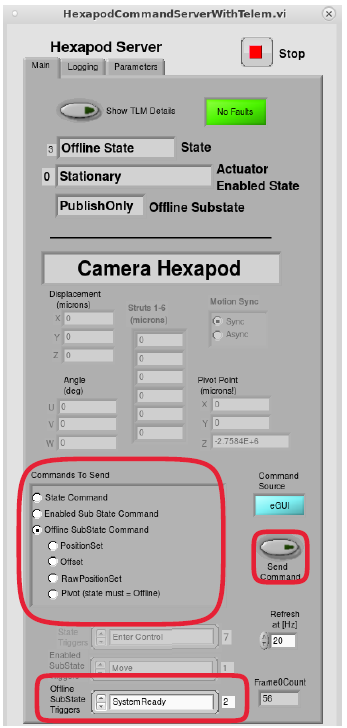
\includegraphics[width=1.79167in,height=\textheight]{jira_imgs/1024.png}

}
\hdashrule[0.5ex]{\textwidth}{1pt}{3mm}
  Expected Result \\
{\footnotesize
The system transitions from the OfflineState/PublishOnly substate to the
OfflineState/AvailableState substate and the Command Source says eGUI.\\
\strut \\

}
\hdashrule[0.5ex]{\textwidth}{1pt}{3mm}
  Actual Result \\
{\footnotesize
worked.

}
\begin{tabular}{p{2cm}p{14cm}}
\toprule
Step 7 & Step Execution Status: \textbf{ Pass } \\ \hline
\end{tabular}
 Description \\
{\footnotesize
\textbf{Transition from OFFLINE State to STANDBY State.}

\hfill\break

On \textbf{Commands to Send}, select the \textbf{State Commands~}radio
button\textbf{.}

On \textbf{State Triggers}, scroll and select \textbf{Enter Control}.

Finally,\textbf{~}click on the \textbf{Send Command} button.

\hfill\break

The Hexapod should go to \textbf{STANDBY} state.

\hfill\break
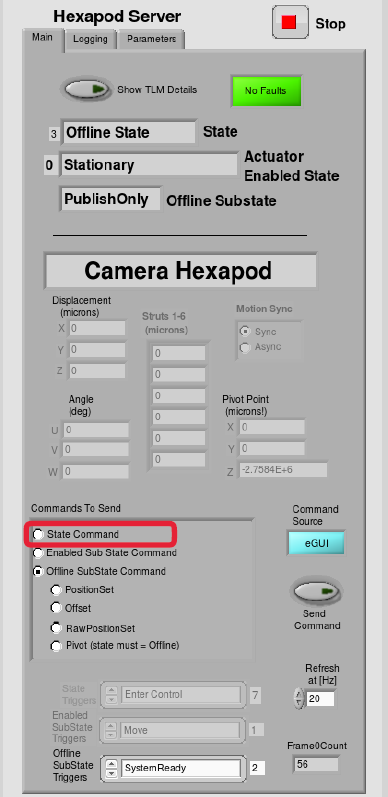
\includegraphics[width=1.79167in,height=\textheight]{jira_imgs/1028.png}

}
\hdashrule[0.5ex]{\textwidth}{1pt}{3mm}
  Expected Result \\
{\footnotesize
The system transitions to the Standby state and the primary state
display box at the top of the Main says Standby state.

}
\hdashrule[0.5ex]{\textwidth}{1pt}{3mm}
  Actual Result \\
{\footnotesize
worked

}
\begin{tabular}{p{2cm}p{14cm}}
\toprule
Step 8 & Step Execution Status: \textbf{ Pass } \\ \hline
\end{tabular}
 Description \\
{\footnotesize
\textbf{Transition from STANDBY State to DISABLED State.}

\hfill\break

On \textbf{Commands to Send}, select the \textbf{State Commands~}radio
button.

On \textbf{State Triggers}, scroll and select the \textbf{Start~}option.

Click on the \textbf{Send Command} button.

\hfill\break

The Hexapod should go to DISABLED state.

}
\hdashrule[0.5ex]{\textwidth}{1pt}{3mm}
  Expected Result \\
{\footnotesize
The system transitions into DISABLED State and the current configuration
parameters are maintained from the default parameters or from the
previous DDS start command.

}
\hdashrule[0.5ex]{\textwidth}{1pt}{3mm}
  Actual Result \\
{\footnotesize
worked

}
\begin{tabular}{p{2cm}p{14cm}}
\toprule
Step 9 & Step Execution Status: \textbf{ Pass } \\ \hline
\end{tabular}
 Description \\
{\footnotesize
\textbf{Transition from DISABLED State to ENABLED State.}

On \textbf{Commands to Send}, select the \textbf{State Commands~}radio
button.

On \textbf{State Triggers}, scroll and select the
\textbf{Enabled~}option.

Click on the \textbf{Send Command~}button.

The Hexapod should go to ENABLED state.

}
\hdashrule[0.5ex]{\textwidth}{1pt}{3mm}
  Expected Result \\
{\footnotesize
The system transitions into the ENABLED State/Stationary sub-state, the
motor drives are enabled and motion can be commanded.

}
\hdashrule[0.5ex]{\textwidth}{1pt}{3mm}
  Actual Result \\
{\footnotesize
worked.\\
\strut \\

}
\begin{tabular}{p{2cm}p{14cm}}
\toprule
Step 10 & Step Execution Status: \textbf{ Not Executed } \\ \hline
\end{tabular}
 Description \\
{\footnotesize
\textless conditional state\textgreater{}\\
\strut \\
\textbf{Recovering from a FAULT State}\\
\strut \\
If a fault occurs in any of the other states, the system will
automatically transition to the FAULT State.\\
While in the Fault state, select the \textbf{clearError} option in the
\textbf{State Triggers~}option list. Then, click on the \textbf{Send
Command~}button\textbf{.}\\
\strut \\
\ul{Note:} If the fault that occurs goes through the interlock system,
reset the safety relay switch and send a \textbf{clearError} command.

}
\hdashrule[0.5ex]{\textwidth}{1pt}{3mm}
  Expected Result \\
{\footnotesize
The system transitions back to the STANDBY state. (Go back to Step 8)

}
\hdashrule[0.5ex]{\textwidth}{1pt}{3mm}
  Actual Result \\
{\footnotesize

}
\begin{tabular}{p{2cm}p{14cm}}
\toprule
Step 11 & Step Execution Status: \textbf{ Not Executed } \\ \hline
\end{tabular}
 Description \\
{\footnotesize
\textbf{Section 3.1.1 of the attached Software Acceptance Test
Procedure\\
Test Sequence \#1 - Synchronous PositionSet and Move Commands}\\
\strut \\
With the synchronous button enabled and in enabled/stationary state,
send a positionSet command of (2000um, -3500um, 200um, .01 deg, -.05deg,
.002deg) using the EUI.

}
\hdashrule[0.5ex]{\textwidth}{1pt}{3mm}
  Test Data \\
 {\footnotesize
\textbf{Deviation:~}There is no positionSet command anymore. Hexapod
moves not immediately when a move command is sent.\\
The pivot position is shown in the GUI. Please mention this in the
results. Use the MOOG pivot point for comparability with the previous
results.

}
\hdashrule[0.5ex]{\textwidth}{1pt}{3mm}
  Expected Result \\
{\footnotesize
\begin{itemize}
\tightlist
\item
  The hexapod moves to the last commanded position of (2000um, -3500um,
  200um, .01 deg, -.05deg, .002deg)
\item
  The actuators complete the move at nearly the same time as seen on the
  motion-complete lights on the telemetry screen.
\end{itemize}

}
\hdashrule[0.5ex]{\textwidth}{1pt}{3mm}
  Actual Result \\
{\footnotesize

}
\begin{tabular}{p{2cm}p{14cm}}
\toprule
Step 12 & Step Execution Status: \textbf{ Not Executed } \\ \hline
\end{tabular}
 Description \\
{\footnotesize
Record the corresponding thermal sensors and verify they are below 19
deg C. If they are above 19 deg C, wait until they are below 19 deg C to
perform the following steps.

}
\hdashrule[0.5ex]{\textwidth}{1pt}{3mm}
  Expected Result \\
{\footnotesize
All actuators are below 19 deg C.

}
\hdashrule[0.5ex]{\textwidth}{1pt}{3mm}
  Actual Result \\
{\footnotesize

}
\begin{tabular}{p{2cm}p{14cm}}
\toprule
Step 13 & Step Execution Status: \textbf{ Not Executed } \\ \hline
\end{tabular}
 Description \\
{\footnotesize
\textbf{Section 3.1.1 of the attached Software Acceptance Test
Procedure\\
Test Sequence \#2 - Pivot, PositionSet and Move Commands}\\
\strut \\
In enabled/stationary state and at the last commanded position of
(2000um, -3500um, 200um, .01 deg, -.05deg, .002deg), change the pivot
point from the default location to (0,0,0) using the EUI.

}
\hdashrule[0.5ex]{\textwidth}{1pt}{3mm}
  Expected Result \\
{\footnotesize
The actuator positions do not change, but the hexapod position is
(-407um, -3982um, 199um, 0.01deg, -0.05deg, 0.002deg).

}
\hdashrule[0.5ex]{\textwidth}{1pt}{3mm}
  Actual Result \\
{\footnotesize

}
\begin{tabular}{p{2cm}p{14cm}}
\toprule
Step 14 & Step Execution Status: \textbf{ Not Executed } \\ \hline
\end{tabular}
 Description \\
{\footnotesize
In the enabled/stationary state, send a move command of (2000um,
-3500um, 200um, .01 deg, -.05deg, .002deg) using the EUI.

}
\hdashrule[0.5ex]{\textwidth}{1pt}{3mm}
  Expected Result \\
{\footnotesize
\begin{itemize}
\tightlist
\item
  The hexapod moves to the commanded position of (2000um, -3500um,
  200um, .01 deg, -.05deg, .002deg)
\item
  The actuators change position to account for the new pivot point.
\end{itemize}

}
\hdashrule[0.5ex]{\textwidth}{1pt}{3mm}
  Actual Result \\
{\footnotesize

}
\begin{tabular}{p{2cm}p{14cm}}
\toprule
Step 15 & Step Execution Status: \textbf{ Not Executed } \\ \hline
\end{tabular}
 Description \\
{\footnotesize
Record the corresponding thermal sensors and verify they are below 19
deg C. If they are above 19 deg C, wait until they are below 19 deg C to
perform the following steps.~

}
\hdashrule[0.5ex]{\textwidth}{1pt}{3mm}
  Expected Result \\
{\footnotesize
All actuators are below 19 deg C.

}
\hdashrule[0.5ex]{\textwidth}{1pt}{3mm}
  Actual Result \\
{\footnotesize

}
\begin{tabular}{p{2cm}p{14cm}}
\toprule
Step 16 & Step Execution Status: \textbf{ Not Executed } \\ \hline
\end{tabular}
 Description \\
{\footnotesize
\textbf{Section 3.1.1 of the attached Software Acceptance Test
Procedure\\
Test Sequence \#4 - Synchronous Offset and Move Commands}\\
\strut \\
With the synchronous button enabled and in enabled/stationary state,
send a move command of (500um, 800um, 200um, 0 deg, 0 deg, 0 deg).

}
\hdashrule[0.5ex]{\textwidth}{1pt}{3mm}
  Expected Result \\
{\footnotesize

}
\hdashrule[0.5ex]{\textwidth}{1pt}{3mm}
  Actual Result \\
{\footnotesize

}
\begin{tabular}{p{2cm}p{14cm}}
\toprule
Step 17 & Step Execution Status: \textbf{ Not Executed } \\ \hline
\end{tabular}
 Description \\
{\footnotesize
With the synchronous button enabled and in enabled/stationary state,
send an offset command of (0um, 0um, 2000um, 0 deg, 0 deg, 0 deg).~

}
\hdashrule[0.5ex]{\textwidth}{1pt}{3mm}
  Expected Result \\
{\footnotesize
The hexapod moves only 2000um in Z from the previous position. Since the
test is done in synchronous mode, the actuators are expected to complete
the move at nearly the same time as seen on the motion-complete lights
on the telemetry screen.

}
\hdashrule[0.5ex]{\textwidth}{1pt}{3mm}
  Actual Result \\
{\footnotesize

}
\begin{tabular}{p{2cm}p{14cm}}
\toprule
Step 18 & Step Execution Status: \textbf{ Not Executed } \\ \hline
\end{tabular}
 Description \\
{\footnotesize
Record the corresponding thermal sensors and verify they are below 19
deg C. If they are above 19 deg C, wait until they are below 19 deg C to
perform the following steps.~

}
\hdashrule[0.5ex]{\textwidth}{1pt}{3mm}
  Expected Result \\
{\footnotesize
All actuators are below 19 deg C.

}
\hdashrule[0.5ex]{\textwidth}{1pt}{3mm}
  Actual Result \\
{\footnotesize

}
\begin{tabular}{p{2cm}p{14cm}}
\toprule
Step 19 & Step Execution Status: \textbf{ Not Executed } \\ \hline
\end{tabular}
 Description \\
{\footnotesize
\textbf{Instead of Asynchronous Test}\\
{With the synchronous button enabled and in enabled/stationary
state,}{\textbf{~}}{s}end a move command of (0um, 0um, 0um, 0.1deg,
0deg, 0deg)

}
\hdashrule[0.5ex]{\textwidth}{1pt}{3mm}
  Expected Result \\
{\footnotesize
The hexapod moves to the commanded position of (0um, 0um, 0um, 0.1deg,
0deg, 0deg)

}
\hdashrule[0.5ex]{\textwidth}{1pt}{3mm}
  Actual Result \\
{\footnotesize

}
\begin{tabular}{p{2cm}p{14cm}}
\toprule
Step 20 & Step Execution Status: \textbf{ Not Executed } \\ \hline
\end{tabular}
 Description \\
{\footnotesize
With the synchronous button enabled and in enabled/stationary
state,\textbf{~}send a move command of (0um, 0um, 0um, 0deg, 0.1deg,
0deg)

}
\hdashrule[0.5ex]{\textwidth}{1pt}{3mm}
  Expected Result \\
{\footnotesize
The hexapod moves to the commanded position of (0um, 0um, 0um, 0deg,
0.1deg, 0deg).

}
\hdashrule[0.5ex]{\textwidth}{1pt}{3mm}
  Actual Result \\
{\footnotesize

}
\begin{tabular}{p{2cm}p{14cm}}
\toprule
Step 21 & Step Execution Status: \textbf{ Not Executed } \\ \hline
\end{tabular}
 Description \\
{\footnotesize
With the synchronous button enabled and in enabled/stationary
state,\textbf{~}send a move command of (0um, 0um, 0um, 0deg, 0.1deg,
0.1deg)

}
\hdashrule[0.5ex]{\textwidth}{1pt}{3mm}
  Expected Result \\
{\footnotesize
The hexapod moves to the commanded position of (0um, 0um, 0um, 0deg,
0.1deg, 0.1deg).

}
\hdashrule[0.5ex]{\textwidth}{1pt}{3mm}
  Actual Result \\
{\footnotesize

}
\begin{tabular}{p{2cm}p{14cm}}
\toprule
Step 22 & Step Execution Status: \textbf{ Not Executed } \\ \hline
\end{tabular}
 Description \\
{\footnotesize
Record the corresponding thermal sensors and verify they are below 19
deg C. If they are above 19 deg C, wait until they are below 19 deg C to
perform the following steps.~

}
\hdashrule[0.5ex]{\textwidth}{1pt}{3mm}
  Expected Result \\
{\footnotesize
All actuators are below 19 deg C.

}
\hdashrule[0.5ex]{\textwidth}{1pt}{3mm}
  Actual Result \\
{\footnotesize

}
\begin{tabular}{p{2cm}p{14cm}}
\toprule
Step 23 & Step Execution Status: \textbf{ Not Executed } \\ \hline
\end{tabular}
 Description \\
{\footnotesize
\textbf{Section 3.1.1 of the attached Software Acceptance Test
Procedure\\
Test Sequence \#5 - Stop Commands}\\
\strut \\
In enabled/stationary state, send a move command of (0um, 0um, 5000um, 0
deg, 0 deg, 0 deg).

}
\hdashrule[0.5ex]{\textwidth}{1pt}{3mm}
  Expected Result \\
{\footnotesize
The hexapod starts to move to the commanded position.

}
\hdashrule[0.5ex]{\textwidth}{1pt}{3mm}
  Actual Result \\
{\footnotesize

}
\begin{tabular}{p{2cm}p{14cm}}
\toprule
Step 24 & Step Execution Status: \textbf{ Not Executed } \\ \hline
\end{tabular}
 Description \\
{\footnotesize
Wait 3s.

}
\hdashrule[0.5ex]{\textwidth}{1pt}{3mm}
  Expected Result \\
{\footnotesize

}
\hdashrule[0.5ex]{\textwidth}{1pt}{3mm}
  Actual Result \\
{\footnotesize

}
\begin{tabular}{p{2cm}p{14cm}}
\toprule
Step 25 & Step Execution Status: \textbf{ Not Executed } \\ \hline
\end{tabular}
 Description \\
{\footnotesize
Send the stop command.~

}
\hdashrule[0.5ex]{\textwidth}{1pt}{3mm}
  Expected Result \\
{\footnotesize
The hexapod quickly comes to a stop prior to reaching the commanded
position.

}
\hdashrule[0.5ex]{\textwidth}{1pt}{3mm}
  Actual Result \\
{\footnotesize

}
\begin{tabular}{p{2cm}p{14cm}}
\toprule
Step 26 & Step Execution Status: \textbf{ Pass } \\ \hline
\end{tabular}
 Description \\
{\footnotesize
\textbf{{Test Sequence \#6}{~}{--}{~}{RawPositionSet Commands}}

\begin{itemize}
\tightlist
\item
  {In enabled/stationary state, send a rawPositionSet command of
  (1000um, 1000um,}{1000um, 50um, 50um, 50um).}{~}
\item
  {Confirm that no motion occurs.}
\item
  {Send a move command. }
\item
  {Confirm that all actuators move to the position values specified
  in}{~the rawPositionSet command.}
\end{itemize}

}
\hdashrule[0.5ex]{\textwidth}{1pt}{3mm}
  Expected Result \\
{\footnotesize
The CamHex reaches the expected position.

}
\hdashrule[0.5ex]{\textwidth}{1pt}{3mm}
  Actual Result \\
{\footnotesize
Deviation: Command to (100um, 100um,100um, 50um, 50um, 50um) for safety
reasons.\\
Hexapod reached the commanded position. -\/-\textgreater{} pass

}
\begin{tabular}{p{2cm}p{14cm}}
\toprule
Step 27 & Step Execution Status: \textbf{ Not Executed } \\ \hline
\end{tabular}
 Description \\
{\footnotesize
\textbf{Section 3.3.1 EUI Tests of the attached Software Acceptance Test
Procedure}\\
At startup, confirm that the system starts in the Offline/PublishOnly
state.

}
\hdashrule[0.5ex]{\textwidth}{1pt}{3mm}
  Expected Result \\
{\footnotesize
The CamHex starts in the Offline/PublishOnly state.

}
\hdashrule[0.5ex]{\textwidth}{1pt}{3mm}
  Actual Result \\
{\footnotesize

}
\begin{tabular}{p{2cm}p{14cm}}
\toprule
Step 28 & Step Execution Status: \textbf{ Not Executed } \\ \hline
\end{tabular}
 Description \\
{\footnotesize
Send an offline substate trigger of systemReady.

}
\hdashrule[0.5ex]{\textwidth}{1pt}{3mm}
  Expected Result \\
{\footnotesize
The system transitions into the Offline/Available substate.

}
\hdashrule[0.5ex]{\textwidth}{1pt}{3mm}
  Actual Result \\
{\footnotesize

}
\begin{tabular}{p{2cm}p{14cm}}
\toprule
Step 29 & Step Execution Status: \textbf{ Not Executed } \\ \hline
\end{tabular}
 Description \\
{\footnotesize
Send an EnterControl trigger.

}
\hdashrule[0.5ex]{\textwidth}{1pt}{3mm}
  Expected Result \\
{\footnotesize
The system transitions from Offline/Available to Standby state.

}
\hdashrule[0.5ex]{\textwidth}{1pt}{3mm}
  Actual Result \\
{\footnotesize

}
\begin{tabular}{p{2cm}p{14cm}}
\toprule
Step 30 & Step Execution Status: \textbf{ Not Executed } \\ \hline
\end{tabular}
 Description \\
{\footnotesize
Send a Start trigger.

}
\hdashrule[0.5ex]{\textwidth}{1pt}{3mm}
  Expected Result \\
{\footnotesize
The system transitions from Standby to Disabled state.

}
\hdashrule[0.5ex]{\textwidth}{1pt}{3mm}
  Actual Result \\
{\footnotesize

}
\begin{tabular}{p{2cm}p{14cm}}
\toprule
Step 31 & Step Execution Status: \textbf{ Not Executed } \\ \hline
\end{tabular}
 Description \\
{\footnotesize
Send an Enable trigger.

}
\hdashrule[0.5ex]{\textwidth}{1pt}{3mm}
  Expected Result \\
{\footnotesize
The system transitions from Disabled to Enabled state.

}
\hdashrule[0.5ex]{\textwidth}{1pt}{3mm}
  Actual Result \\
{\footnotesize

}
\begin{tabular}{p{2cm}p{14cm}}
\toprule
Step 32 & Step Execution Status: \textbf{ Not Executed } \\ \hline
\end{tabular}
 Description \\
{\footnotesize
Send a Disable trigger.

}
\hdashrule[0.5ex]{\textwidth}{1pt}{3mm}
  Expected Result \\
{\footnotesize
The system transitions from Enabled to Disabled state.

}
\hdashrule[0.5ex]{\textwidth}{1pt}{3mm}
  Actual Result \\
{\footnotesize

}
\begin{tabular}{p{2cm}p{14cm}}
\toprule
Step 33 & Step Execution Status: \textbf{ Not Executed } \\ \hline
\end{tabular}
 Description \\
{\footnotesize
Send a Standby trigger.

}
\hdashrule[0.5ex]{\textwidth}{1pt}{3mm}
  Expected Result \\
{\footnotesize
The system transitions from Disabled state to Standby state.

}
\hdashrule[0.5ex]{\textwidth}{1pt}{3mm}
  Actual Result \\
{\footnotesize

}
\begin{tabular}{p{2cm}p{14cm}}
\toprule
Step 34 & Step Execution Status: \textbf{ Not Executed } \\ \hline
\end{tabular}
 Description \\
{\footnotesize
Send a exitControl trigger.

}
\hdashrule[0.5ex]{\textwidth}{1pt}{3mm}
  Expected Result \\
{\footnotesize
The system transitions from Standby state to Offline state.

}
\hdashrule[0.5ex]{\textwidth}{1pt}{3mm}
  Actual Result \\
{\footnotesize

}
\begin{tabular}{p{2cm}p{14cm}}
\toprule
Step 35 & Step Execution Status: \textbf{ Not Executed } \\ \hline
\end{tabular}
 Description \\
{\footnotesize
Return to the Enabled state and trip the safety interlock switch.

}
\hdashrule[0.5ex]{\textwidth}{1pt}{3mm}
  Expected Result \\
{\footnotesize
The system transitions to Fault state.

}
\hdashrule[0.5ex]{\textwidth}{1pt}{3mm}
  Actual Result \\
{\footnotesize

}
\begin{tabular}{p{2cm}p{14cm}}
\toprule
Step 36 & Step Execution Status: \textbf{ Not Executed } \\ \hline
\end{tabular}
 Description \\
{\footnotesize
Reset the safety interlock and send a ClearError trigger.

}
\hdashrule[0.5ex]{\textwidth}{1pt}{3mm}
  Expected Result \\
{\footnotesize
\begin{itemize}
\tightlist
\item
  The EUI, upon receiving the ¨clearError¨ trigger, transitions from
  FaultState to OfflineState/PublishOnly when the system was in any of
  the OfflineStates before the error occurred.~
\item
  The EUI, upon receiving the "clearError" trigger, transitions to
  StandbyState when it was in EnableState or DisableState before the
  error occurred.
\end{itemize}

}
\hdashrule[0.5ex]{\textwidth}{1pt}{3mm}
  Actual Result \\
{\footnotesize

}
\begin{tabular}{p{2cm}p{14cm}}
\toprule
Step 37 & Step Execution Status: \textbf{ Not Executed } \\ \hline
\end{tabular}
 Description \\
{\footnotesize
\textbf{Section 4.1 Hexapod Events of the attached Software Acceptance
Test Procedure}\\
\strut \\
In the Enabled/Stationary state, unplug a motor encoder cable for one of
the actuators.

}
\hdashrule[0.5ex]{\textwidth}{1pt}{3mm}
  Test Data \\
 {\footnotesize
\textbf{Deviation:~}Perform the following set of steps using the EUI
instead of the DDS and verify the events are displayed on the EUI.

}
\hdashrule[0.5ex]{\textwidth}{1pt}{3mm}
  Expected Result \\
{\footnotesize
A Drive Fault error event is created and the system transitions to Fault
state.

}
\hdashrule[0.5ex]{\textwidth}{1pt}{3mm}
  Actual Result \\
{\footnotesize

}
\begin{tabular}{p{2cm}p{14cm}}
\toprule
Step 38 & Step Execution Status: \textbf{ Not Executed } \\ \hline
\end{tabular}
 Description \\
{\footnotesize
Send the "clearError" trigger and transition the state machine to the
Enabled/Stationary state.

}
\hdashrule[0.5ex]{\textwidth}{1pt}{3mm}
  Expected Result \\
{\footnotesize
The state machine is in the Enabled/Stationary state and therefore ready
to be commanded.

}
\hdashrule[0.5ex]{\textwidth}{1pt}{3mm}
  Actual Result \\
{\footnotesize

}
\begin{tabular}{p{2cm}p{14cm}}
\toprule
Step 39 & Step Execution Status: \textbf{ Not Executed } \\ \hline
\end{tabular}
 Description \\
{\footnotesize
In the Enabled/Stationary state, unplug a linear encoder cable for one
of the actuators.~

}
\hdashrule[0.5ex]{\textwidth}{1pt}{3mm}
  Expected Result \\
{\footnotesize
A Drive Fault error event is created and the system transitions to Fault
state.

}
\hdashrule[0.5ex]{\textwidth}{1pt}{3mm}
  Actual Result \\
{\footnotesize

}
\begin{tabular}{p{2cm}p{14cm}}
\toprule
Step 40 & Step Execution Status: \textbf{ Not Executed } \\ \hline
\end{tabular}
 Description \\
{\footnotesize
Send the "clearError" trigger and bring the system to the
Enabled/Stationary state.

}
\hdashrule[0.5ex]{\textwidth}{1pt}{3mm}
  Expected Result \\
{\footnotesize
The system is in the Enabled/Stationary state and ready to be commanded.

}
\hdashrule[0.5ex]{\textwidth}{1pt}{3mm}
  Actual Result \\
{\footnotesize

}
\begin{tabular}{p{2cm}p{14cm}}
\toprule
Step 41 & Step Execution Status: \textbf{ Not Executed } \\ \hline
\end{tabular}
 Description \\
{\footnotesize
In the Enabled/Stationary state, unplug a linear encoder cable for one
of the actuators.~

}
\hdashrule[0.5ex]{\textwidth}{1pt}{3mm}
  Expected Result \\
{\footnotesize
A Drive Fault error event is created and the system transitions to Fault
state.

}
\hdashrule[0.5ex]{\textwidth}{1pt}{3mm}
  Actual Result \\
{\footnotesize

}
\begin{tabular}{p{2cm}p{14cm}}
\toprule
Step 42 & Step Execution Status: \textbf{ Not Executed } \\ \hline
\end{tabular}
 Description \\
{\footnotesize
Send the "clearError" trigger and bring the system to the
Enabled/Stationary state.

}
\hdashrule[0.5ex]{\textwidth}{1pt}{3mm}
  Expected Result \\
{\footnotesize
The system is in the Enabled/Stationary state and ready to be commanded.

}
\hdashrule[0.5ex]{\textwidth}{1pt}{3mm}
  Actual Result \\
{\footnotesize

}
\begin{tabular}{p{2cm}p{14cm}}
\toprule
Step 43 & Step Execution Status: \textbf{ Not Executed } \\ \hline
\end{tabular}
 Description \\
{\footnotesize
Unplug a motor power cable from one of the actuators and command a
PositionSet/Move.~

}
\hdashrule[0.5ex]{\textwidth}{1pt}{3mm}
  Expected Result \\
{\footnotesize
A Following Error event is created and the system transitions to Fault
state.

}
\hdashrule[0.5ex]{\textwidth}{1pt}{3mm}
  Actual Result \\
{\footnotesize

}
\begin{tabular}{p{2cm}p{14cm}}
\toprule
Step 44 & Step Execution Status: \textbf{ Not Executed } \\ \hline
\end{tabular}
 Description \\
{\footnotesize
Send the "clearError" trigger and bring the system to the
Enabled/Stationary state.

}
\hdashrule[0.5ex]{\textwidth}{1pt}{3mm}
  Expected Result \\
{\footnotesize
The system is in the Enabled/Stationary state and ready to be commanded.

}
\hdashrule[0.5ex]{\textwidth}{1pt}{3mm}
  Actual Result \\
{\footnotesize

}
\begin{tabular}{p{2cm}p{14cm}}
\toprule
Step 45 & Step Execution Status: \textbf{ Not Executed } \\ \hline
\end{tabular}
 Description \\
{\footnotesize
Activate an extension limit switch on one of the actuators by removing
the limit switch cover and manually tripping.~

}
\hdashrule[0.5ex]{\textwidth}{1pt}{3mm}
  Expected Result \\
{\footnotesize
An Extended Limit Switch error event is created and the system
transitions into Fault state.

}
\hdashrule[0.5ex]{\textwidth}{1pt}{3mm}
  Actual Result \\
{\footnotesize

}
\begin{tabular}{p{2cm}p{14cm}}
\toprule
Step 46 & Step Execution Status: \textbf{ Not Executed } \\ \hline
\end{tabular}
 Description \\
{\footnotesize
Send the "clearError" trigger and bring the system to the
Enabled/Stationary state.

}
\hdashrule[0.5ex]{\textwidth}{1pt}{3mm}
  Expected Result \\
{\footnotesize
The system is in the Enabled/Stationary state and ready to be commanded.

}
\hdashrule[0.5ex]{\textwidth}{1pt}{3mm}
  Actual Result \\
{\footnotesize

}
\begin{tabular}{p{2cm}p{14cm}}
\toprule
Step 47 & Step Execution Status: \textbf{ Not Executed } \\ \hline
\end{tabular}
 Description \\
{\footnotesize
Activate a retraction limit switch on one of the actuators by removing
the limit switch cover and manually tripping.

}
\hdashrule[0.5ex]{\textwidth}{1pt}{3mm}
  Expected Result \\
{\footnotesize
A Retracted Limit Switch error event is created and the system
transitions into Fault state.

}
\hdashrule[0.5ex]{\textwidth}{1pt}{3mm}
  Actual Result \\
{\footnotesize

}
\begin{tabular}{p{2cm}p{14cm}}
\toprule
Step 48 & Step Execution Status: \textbf{ Not Executed } \\ \hline
\end{tabular}
 Description \\
{\footnotesize
Send the "clearError" trigger and bring the system to the
Enabled/Stationary state.

}
\hdashrule[0.5ex]{\textwidth}{1pt}{3mm}
  Expected Result \\
{\footnotesize
The system is in the Enabled/Stationary state and ready to be commanded.

}
\hdashrule[0.5ex]{\textwidth}{1pt}{3mm}
  Actual Result \\
{\footnotesize

}
\begin{tabular}{p{2cm}p{14cm}}
\toprule
Step 49 & Step Execution Status: \textbf{ Not Executed } \\ \hline
\end{tabular}
 Description \\
{\footnotesize
Unplug the Ethercat cable between the control PC and the first Copley
XE2 drive.

}
\hdashrule[0.5ex]{\textwidth}{1pt}{3mm}
  Expected Result \\
{\footnotesize
An Ethercat Lost event is created and the system transitions to Fault
state.

}
\hdashrule[0.5ex]{\textwidth}{1pt}{3mm}
  Actual Result \\
{\footnotesize

}
\begin{tabular}{p{2cm}p{14cm}}
\toprule
Step 50 & Step Execution Status: \textbf{ Not Executed } \\ \hline
\end{tabular}
 Description \\
{\footnotesize
Send the "clearError" trigger and bring the system to the
Enabled/Stationary state.

}
\hdashrule[0.5ex]{\textwidth}{1pt}{3mm}
  Expected Result \\
{\footnotesize
The system is in the Enabled/Stationary state and ready to be commanded.

}
\hdashrule[0.5ex]{\textwidth}{1pt}{3mm}
  Actual Result \\
{\footnotesize

}

\paragraph{ LVV-T1600 - Integration of Camera Hexapod with SAL }\mbox{}\\

Version \textbf{2}.
Status \textbf{Approved}.
Open  \href{https://jira.lsstcorp.org/secure/Tests.jspa#/testCase/LVV-T1600}{\textit{ LVV-T1600 } }
test case in Jira.

The objective of this test case is to re-verify the functional
requirements of the camera hexapod\textquotesingle s software, after
shipment of the hardware from the vendor\textquotesingle s facility to
the Summit, as defined in \citeds{LTS-206} and \citeds{LTS-160}. This test case will only
exercise the functionality that was executed previously and meets the
following criteria:

\begin{itemize}
\tightlist
\item
  Only requires the use of Russell\textquotesingle s code to replace
  MOOG\textquotesingle s middleware code
\item
  Only requires the camera hexapod to be operable
\item
  Only requires command through the CSC after the cRIO is switched from
  GUI mode to DDS mode
\item
  Only requires testing of the synchronous mode

  \begin{itemize}
  \tightlist
  \item
    \textbf{Asynchronous mode is not a standard mode of operation}
  \end{itemize}
\item
  This test case can be executed with or without the camera rotator to
  be loaded with the camera simulated mass or actual camera hardware
\end{itemize}

The software functional requirements were previously verified during the
test campaign by the vendor at the vendor\textquotesingle s facility and
accepted by LSST during the Factory Acceptance Test review. The test
procedure used during the vendor\textquotesingle s acceptance testing is
the \emph{LSST Hexapods-Rotator Software Acceptance Test Procedure}
which is attached to this test case. The test steps of this test case
are derived from the same procedure, but the order of the steps have
been changed to reflect the \emph{Proposal of Hexapod Test~on Dec.
2019~}Confluence page which can be found linked in the Traceability
tab.\\
\strut \\
See the attached \emph{LSST Rotator Hexapod\textquotesingle s Manual}
for more information on how to operate the hexapod.

\textbf{ Preconditions}:\\
Prior to the execution of this test case to re-verify the Camera Hexapod
hardware functional requirements, the following Summit tasks must be
completed:

\begin{itemize}
\tightlist
\item
  The Hexapod has been installed on the camera cart

  \begin{itemize}
  \tightlist
  \item
    \url{https://jira.lsstcorp.org/browse/SUMMIT-3224}
  \end{itemize}
\item
  The Hexapod Controller has been deployed on the summit

  \begin{itemize}
  \tightlist
  \item
    \url{https://jira.lsstcorp.org/browse/SUMMIT-3229}
  \end{itemize}
\item
  Boxes for the Hexapod have been transported to the 3rd level

  \begin{itemize}
  \tightlist
  \item
    \url{https://jira.lsstcorp.org/browse/SUMMIT-3230}
  \end{itemize}
\item
  All Hexapod cables and cabinets have been prepared for integration
  with camera cart

  \begin{itemize}
  \tightlist
  \item
    \url{https://jira.lsstcorp.org/browse/SUMMIT-3231}
  \end{itemize}
\item
  The offset has been installed onto the integrating structure

  \begin{itemize}
  \tightlist
  \item
    \url{https://jira.lsstcorp.org/browse/SUMMIT-3293}
  \end{itemize}
\item
  The Camera Hexapod electrical connections have been tested

  \begin{itemize}
  \tightlist
  \item
    \url{https://jira.lsstcorp.org/browse/SUMMIT-3294}
  \end{itemize}
\end{itemize}

Execution status: {\bf Not Executed }

Final comment:\\


Detailed steps results:

\begin{tabular}{p{2cm}p{14cm}}
\toprule
Step 1 & Step Execution Status: \textbf{ Not Executed } \\ \hline
\end{tabular}
 Description \\
{\footnotesize
\textbf{STARTING THE EUI}\\
\strut \\
Double click the Hexapod GUI Viewer desktop icon on the computer.

\begin{itemize}
\tightlist
\item
  This can be done on the Dell Management PC or another computer on the
  same network
\end{itemize}

}
\hdashrule[0.5ex]{\textwidth}{1pt}{3mm}
  Expected Result \\
{\footnotesize
A prompt to enter a password is shown.~

}
\hdashrule[0.5ex]{\textwidth}{1pt}{3mm}
  Actual Result \\
{\footnotesize

}
\begin{tabular}{p{2cm}p{14cm}}
\toprule
Step 2 & Step Execution Status: \textbf{ Not Executed } \\ \hline
\end{tabular}
 Description \\
{\footnotesize
Enter the password "lsst-vnc"

\begin{itemize}
\tightlist
\item
  If the EUI isn\textquotesingle t automatically up and running when the
  VNC opens, double click on the Hexapod-eGUI icon on the VNC viewer
\end{itemize}

}
\hdashrule[0.5ex]{\textwidth}{1pt}{3mm}
  Expected Result \\
{\footnotesize
The EUI is in the Offline State/PublishOnly substate and is able to
publish through SAL but cannot receive commands.

}
\hdashrule[0.5ex]{\textwidth}{1pt}{3mm}
  Actual Result \\
{\footnotesize

}
\begin{tabular}{p{2cm}p{14cm}}
\toprule
Step 3 & Step Execution Status: \textbf{ Not Executed } \\ \hline
\end{tabular}
 Description \\
{\footnotesize
\textbf{OFFLINESTATE/PUBLISHONLY -\textgreater{}
OFFLINESTATE/AVAILABLESTATE}\\
On the Main tab, select the "Offline SubState Cmd" field in the Commands
to Send section, set the Offline SubState Triggers to "System Ready" and
click on the Send Command button.\\
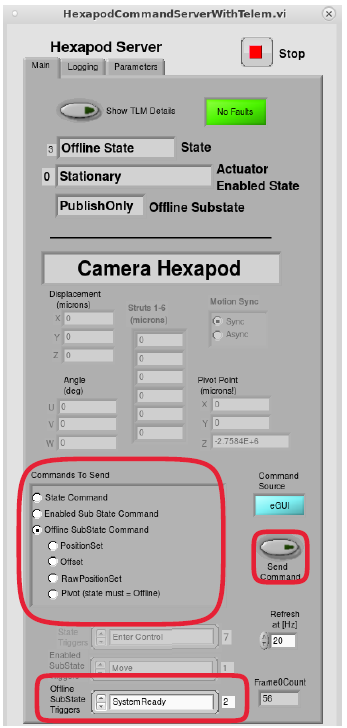
\includegraphics[width=1.79167in,height=\textheight]{jira_imgs/1024.png}

}
\hdashrule[0.5ex]{\textwidth}{1pt}{3mm}
  Expected Result \\
{\footnotesize
The system transitions from the OfflineState/PublishOnly substate to the
OfflineState/AvailableState substate.\\
\strut \\

}
\hdashrule[0.5ex]{\textwidth}{1pt}{3mm}
  Actual Result \\
{\footnotesize

}
\begin{tabular}{p{2cm}p{14cm}}
\toprule
Step 4 & Step Execution Status: \textbf{ Not Executed } \\ \hline
\end{tabular}
 Description \\
{\footnotesize
\textbf{SWITCHING TO DDS MODE}\\
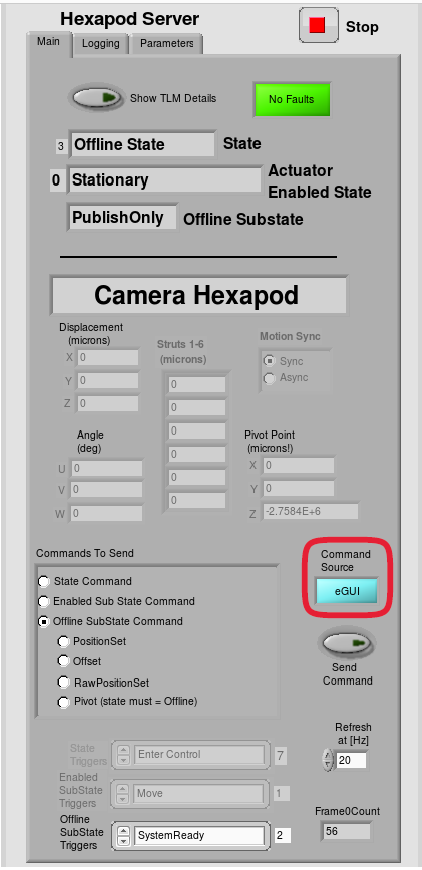
\includegraphics[width=1.6875in,height=\textheight]{jira_imgs/1025.png}If
the Command Source does not show DDS, go to the Parameters tab, select
DDS under the Command Source and click the Set Cmd Source button.\\
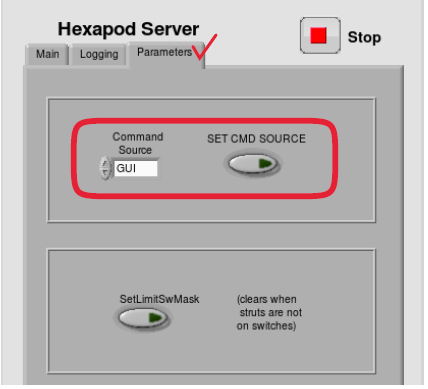
\includegraphics[width=2.34375in,height=\textheight]{jira_imgs/1026.png}\ul{\textbf{Note:}}\textbf{~If
the GUI is used after being set to DDS mode, the system will switch back
the Command Source to GUI and ignore any DDS commands. The Command
Source must show DDS in order to receive DDS commands.}

}
\hdashrule[0.5ex]{\textwidth}{1pt}{3mm}
  Expected Result \\
{\footnotesize
The system is capable of receiving/responding to DDS commands.

}
\hdashrule[0.5ex]{\textwidth}{1pt}{3mm}
  Actual Result \\
{\footnotesize

}
\begin{tabular}{p{2cm}p{14cm}}
\toprule
Step 5 & Step Execution Status: \textbf{ Not Executed } \\ \hline
\end{tabular}
 Description \\
{\footnotesize
\textbf{OFFLINESTATE -\textgreater{} STANDBYSTATE}\\
The system receives an enterControl State Transition command through
DDS.

}
\hdashrule[0.5ex]{\textwidth}{1pt}{3mm}
  Expected Result \\
{\footnotesize
The system transitions into the StandbyState and is capable of
receiving/responding to DDS commands.

}
\hdashrule[0.5ex]{\textwidth}{1pt}{3mm}
  Actual Result \\
{\footnotesize

}
\begin{tabular}{p{2cm}p{14cm}}
\toprule
Step 6 & Step Execution Status: \textbf{ Not Executed } \\ \hline
\end{tabular}
 Description \\
{\footnotesize
\textbf{STANDBYSTATE -\textgreater{} DISABLEDSTATE}\\
From the StandbyState, send a start command through the DDS.

}
\hdashrule[0.5ex]{\textwidth}{1pt}{3mm}
  Expected Result \\
{\footnotesize
The system transitions into DisabledState after receiving/responding to
DDS command and the wrapper in the PXI real time controller looks for
the configuration file.\\
\strut \\
If the configuration file is invalid or out of range, the system will
transition into a Fault State

}
\hdashrule[0.5ex]{\textwidth}{1pt}{3mm}
  Actual Result \\
{\footnotesize

}
\begin{tabular}{p{2cm}p{14cm}}
\toprule
Step 7 & Step Execution Status: \textbf{ Not Executed } \\ \hline
\end{tabular}
 Description \\
{\footnotesize
\textbf{DISABLEDSTATE -\textgreater{} ENABLEDSTATE}\\
From the DisabledState, send an enable state command through the DDS.\\
\textbf{}

}
\hdashrule[0.5ex]{\textwidth}{1pt}{3mm}
  Expected Result \\
{\footnotesize
The system transitions into the EnabledState/Stationary substate, the
motor drives are enabled, motor brakes are released and the system is
capable of receiving/responding to DDS commands.\\
\strut \\

}
\hdashrule[0.5ex]{\textwidth}{1pt}{3mm}
  Actual Result \\
{\footnotesize

}
\begin{tabular}{p{2cm}p{14cm}}
\toprule
Step 8 & Step Execution Status: \textbf{ Not Executed } \\ \hline
\end{tabular}
 Description \\
{\footnotesize
\textbf{FAULTSTATE}\\
If a Fault occurs in any of the other states, the system will
automatically transition to the Fault State. While in the Fault state,
send a clearError command through the DDS.\\
\ul{Note:} If the fault that occurs goes through the interlock system,
reset the safety relay switch and send a clearError command.

}
\hdashrule[0.5ex]{\textwidth}{1pt}{3mm}
  Expected Result \\
{\footnotesize
The system transitions back to the OfflineState/PublishOnly substate and
is not capable of receiving/responding to DDS commands. (Go back to Step
3)

}
\hdashrule[0.5ex]{\textwidth}{1pt}{3mm}
  Actual Result \\
{\footnotesize

}
\begin{tabular}{p{2cm}p{14cm}}
\toprule
Step 9 & Step Execution Status: \textbf{ Not Executed } \\ \hline
\end{tabular}
 Description \\
{\footnotesize
Verify that the thermal sensors are connected and producing telemetry
into the EFD.

}
\hdashrule[0.5ex]{\textwidth}{1pt}{3mm}
  Expected Result \\
{\footnotesize
All actuator temperatures are published to the EFD.

}
\hdashrule[0.5ex]{\textwidth}{1pt}{3mm}
  Actual Result \\
{\footnotesize

}
\begin{tabular}{p{2cm}p{14cm}}
\toprule
Step 10 & Step Execution Status: \textbf{ Not Executed } \\ \hline
\end{tabular}
 Description \\
{\footnotesize
The following steps define what the Jupyter Notebook for this test case
implements. Executing the Jupyter notebook is the only actual command
and control step that needs to be executed.

}
\hdashrule[0.5ex]{\textwidth}{1pt}{3mm}
  Expected Result \\
{\footnotesize
The Jupyter notebook controls the system to run through the steps below.

}
\hdashrule[0.5ex]{\textwidth}{1pt}{3mm}
  Actual Result \\
{\footnotesize

}
\begin{tabular}{p{2cm}p{14cm}}
\toprule
Step 11 & Step Execution Status: \textbf{ Not Executed } \\ \hline
\end{tabular}
 Description \\
{\footnotesize
Verify all the telemetry is being ingested into the EFD.

}
\hdashrule[0.5ex]{\textwidth}{1pt}{3mm}
  Expected Result \\
{\footnotesize
All telemetry defined in the script is being ingested into the EFD.

}
\hdashrule[0.5ex]{\textwidth}{1pt}{3mm}
  Actual Result \\
{\footnotesize

}
\begin{tabular}{p{2cm}p{14cm}}
\toprule
Step 12 & Step Execution Status: \textbf{ Not Executed } \\ \hline
\end{tabular}
 Description \\
{\footnotesize
\textbf{{MOVE TEST}}\\
\textbf{Section 3.1.2 of the attached Software Acceptance Test
Procedure\\
Test Sequence \#1 - Synchronous PositionSet and Move Commands}\\
In enabled/stationary state, send a positionSet command of (0um, 0um,
200um, 0 deg, 0 deg, 0 deg, s).

}
\hdashrule[0.5ex]{\textwidth}{1pt}{3mm}
  Test Data \\
 {\footnotesize
\textbf{Deviation:~}Skip this step. positionSet and move command
replaced by new move command. Now, the hexapod starts movement directly
after receiving the command.

}
\hdashrule[0.5ex]{\textwidth}{1pt}{3mm}
  Expected Result \\
{\footnotesize
The hexapod does not move.

}
\hdashrule[0.5ex]{\textwidth}{1pt}{3mm}
  Actual Result \\
{\footnotesize

}
\begin{tabular}{p{2cm}p{14cm}}
\toprule
Step 13 & Step Execution Status: \textbf{ Not Executed } \\ \hline
\end{tabular}
 Description \\
{\footnotesize
With the synchronous button enabled and in enabled/stationary state,
send a positionSet command of (500um, -500um, 200um, 0.01deg, -0.015deg,
0deg).

}
\hdashrule[0.5ex]{\textwidth}{1pt}{3mm}
  Test Data \\
 {\footnotesize
\textbf{Deviation:~}Skip this step. positionSet and move command
replaced by new move command. Now, the hexapod starts movement directly
after receiving the command.

}
\hdashrule[0.5ex]{\textwidth}{1pt}{3mm}
  Expected Result \\
{\footnotesize
The hexapod does not move

}
\hdashrule[0.5ex]{\textwidth}{1pt}{3mm}
  Actual Result \\
{\footnotesize

}
\begin{tabular}{p{2cm}p{14cm}}
\toprule
Step 14 & Step Execution Status: \textbf{ Not Executed } \\ \hline
\end{tabular}
 Description \\
{\footnotesize
With the hexapod in in enabled/stationary state sync=True and send the
move command of (x= 500um,y= -500um, z=200um, u=0.01deg, v=-0.015deg,
w=0deg).

}
\hdashrule[0.5ex]{\textwidth}{1pt}{3mm}
  Expected Result \\
{\footnotesize
\begin{itemize}
\tightlist
\item
  The hexapod moves to (x= 500um,y= -500um, z=200um, u=0.01deg,
  v=-0.015deg, w=0deg)
\item
  Since the Hexapod is in synchronous mode, the actuators complete the
  move at nearly the same time.
\end{itemize}

}
\hdashrule[0.5ex]{\textwidth}{1pt}{3mm}
  Actual Result \\
{\footnotesize

}
\begin{tabular}{p{2cm}p{14cm}}
\toprule
Step 15 & Step Execution Status: \textbf{ Not Executed } \\ \hline
\end{tabular}
 Description \\
{\footnotesize
Record the corresponding DDS events that were generated.

}
\hdashrule[0.5ex]{\textwidth}{1pt}{3mm}
  Expected Result \\
{\footnotesize
\begin{itemize}
\tightlist
\item
  The controllerState.enabledSubstate goes to MOVING\_POINT\_TO\_POINT
  when the move begins and STATIONARY when the move ends.
\item
  An inPosition event is generated when the move is complete
\end{itemize}

}
\hdashrule[0.5ex]{\textwidth}{1pt}{3mm}
  Actual Result \\
{\footnotesize

}
\begin{tabular}{p{2cm}p{14cm}}
\toprule
Step 16 & Step Execution Status: \textbf{ Not Executed } \\ \hline
\end{tabular}
 Description \\
{\footnotesize
Wait 39 seconds.

}
\hdashrule[0.5ex]{\textwidth}{1pt}{3mm}
  Expected Result \\
{\footnotesize

}
\hdashrule[0.5ex]{\textwidth}{1pt}{3mm}
  Actual Result \\
{\footnotesize

}
\begin{tabular}{p{2cm}p{14cm}}
\toprule
Step 17 & Step Execution Status: \textbf{ Not Executed } \\ \hline
\end{tabular}
 Description \\
{\footnotesize
Record the corresponding thermal sensors and verify they are below 19
deg C. If they are above 19 deg C, wait until they are below 19 deg C to
perform the following steps.

}
\hdashrule[0.5ex]{\textwidth}{1pt}{3mm}
  Expected Result \\
{\footnotesize
All actuators are below 19 deg C.

}
\hdashrule[0.5ex]{\textwidth}{1pt}{3mm}
  Actual Result \\
{\footnotesize

}
\begin{tabular}{p{2cm}p{14cm}}
\toprule
Step 18 & Step Execution Status: \textbf{ Not Executed } \\ \hline
\end{tabular}
 Description \\
{\footnotesize
\textbf{Section 3.1.2 of the attached Software Acceptance Test
Procedure\\
Test Sequence \#5 - Stop Commands}\\
In the enabled/stationary state, send a move command of (x=0um, y=0um,
z=5000um, u=0deg, v=0deg, w=0deg)

}
\hdashrule[0.5ex]{\textwidth}{1pt}{3mm}
  Expected Result \\
{\footnotesize
The hexapod doesn\textquotesingle t move.

}
\hdashrule[0.5ex]{\textwidth}{1pt}{3mm}
  Actual Result \\
{\footnotesize

}
\begin{tabular}{p{2cm}p{14cm}}
\toprule
Step 19 & Step Execution Status: \textbf{ Not Executed } \\ \hline
\end{tabular}
 Description \\
{\footnotesize
Wait 3s.

}
\hdashrule[0.5ex]{\textwidth}{1pt}{3mm}
  Expected Result \\
{\footnotesize

}
\hdashrule[0.5ex]{\textwidth}{1pt}{3mm}
  Actual Result \\
{\footnotesize

}
\begin{tabular}{p{2cm}p{14cm}}
\toprule
Step 20 & Step Execution Status: \textbf{ Not Executed } \\ \hline
\end{tabular}
 Description \\
{\footnotesize
Send a stop command.

}
\hdashrule[0.5ex]{\textwidth}{1pt}{3mm}
  Expected Result \\
{\footnotesize
The hexapod stops before reaching the previously commanded position

}
\hdashrule[0.5ex]{\textwidth}{1pt}{3mm}
  Actual Result \\
{\footnotesize

}
\begin{tabular}{p{2cm}p{14cm}}
\toprule
Step 21 & Step Execution Status: \textbf{ Not Executed } \\ \hline
\end{tabular}
 Description \\
{\footnotesize
Record the corresponding DDS events that were generated.

}
\hdashrule[0.5ex]{\textwidth}{1pt}{3mm}
  Expected Result \\
{\footnotesize
\begin{itemize}
\tightlist
\item
  The controllerState.enabledSubstate goes to CONTROLLED\_STOPPING when
  the stop is requested, then STATIONARY when the hexapod has halted.
\item
  In the EFD the codes for the EnabledSubstate are:

  \begin{itemize}
  \tightlist
  \item
    Stationary=0
  \item
    MovingPointToPoint=1
  \item
    SlewingOrTracking=2
  \item
    ControlledStopping=3
  \item
    Initializing=4
  \item
    Relative=5
  \item
    ConstantVelocity=6
  \end{itemize}
\item
  No inPosition event is generated.
\end{itemize}

}
\hdashrule[0.5ex]{\textwidth}{1pt}{3mm}
  Actual Result \\
{\footnotesize

}
\begin{tabular}{p{2cm}p{14cm}}
\toprule
Step 22 & Step Execution Status: \textbf{ Not Executed } \\ \hline
\end{tabular}
 Description \\
{\footnotesize
Wait 39 seconds.

}
\hdashrule[0.5ex]{\textwidth}{1pt}{3mm}
  Expected Result \\
{\footnotesize

}
\hdashrule[0.5ex]{\textwidth}{1pt}{3mm}
  Actual Result \\
{\footnotesize

}
\begin{tabular}{p{2cm}p{14cm}}
\toprule
Step 23 & Step Execution Status: \textbf{ Not Executed } \\ \hline
\end{tabular}
 Description \\
{\footnotesize
Record the corresponding thermal sensors and verify they are below 19
deg C. If they are above 19 deg C, wait until they are below 19 deg C to
perform the following steps.

}
\hdashrule[0.5ex]{\textwidth}{1pt}{3mm}
  Expected Result \\
{\footnotesize
All actuators are below 19 deg C.

}
\hdashrule[0.5ex]{\textwidth}{1pt}{3mm}
  Actual Result \\
{\footnotesize

}
\begin{tabular}{p{2cm}p{14cm}}
\toprule
Step 24 & Step Execution Status: \textbf{ Not Executed } \\ \hline
\end{tabular}
 Description \\
{\footnotesize
\textbf{Section 3.1.2 of the attached Software Acceptance Test
Procedure\\
Test Sequence \#9 - positionSet and moveLUT}\\
\strut \\
\textbf{Update: Test the "setCompensationMode" command.}\\
\strut \\
In enabled/stationary state, send a move command of (x=0um, y=0um,
z=800um, u=0deg, v=0deg, w=0deg)\\
\strut \\

}
\hdashrule[0.5ex]{\textwidth}{1pt}{3mm}
  Test Data \\
 {\footnotesize
\textbf{Deviation:} There is no "positionSet" and no "moveLUT" command
anymore. "positionSet" and "move" command replaced by new "move"
command. Now, the hexapod starts movement directly after receiving the
command. moveLUT is replaced by a "setCompensationMode".

}
\hdashrule[0.5ex]{\textwidth}{1pt}{3mm}
  Expected Result \\
{\footnotesize
The hexapod moves to the position (x=0um, y=0um, z=800um, u=0deg,
v=0deg, w=0deg) and, since we are moving in synchronous mode, the
actuators complete the move at nearly the same time.

}
\hdashrule[0.5ex]{\textwidth}{1pt}{3mm}
  Actual Result \\
{\footnotesize

}
\begin{tabular}{p{2cm}p{14cm}}
\toprule
Step 25 & Step Execution Status: \textbf{ Not Executed } \\ \hline
\end{tabular}
 Description \\
{\footnotesize
Ensure that MTMount publishes the telescope elevation angle and
MTRotator publishes the rotation angle of the rotator. Either as real
components or through controllers simulating the components.

}
\hdashrule[0.5ex]{\textwidth}{1pt}{3mm}
  Expected Result \\
{\footnotesize
Published telescope elevation and rotator angle.

}
\hdashrule[0.5ex]{\textwidth}{1pt}{3mm}
  Actual Result \\
{\footnotesize

}
\begin{tabular}{p{2cm}p{14cm}}
\toprule
Step 26 & Step Execution Status: \textbf{ Not Executed } \\ \hline
\end{tabular}
 Description \\
{\footnotesize
In enabled/stationary state, set ~"setCompensationMode" command to
enable=True.

}
\hdashrule[0.5ex]{\textwidth}{1pt}{3mm}
  Expected Result \\
{\footnotesize
The hexapod does not move and the
~MTHexapod.command\_setCompensationMode appears as true in the EFD.\\
\strut \\
logevent\_compensatedPosition is sent to the EFD.\\
\strut \\

}
\hdashrule[0.5ex]{\textwidth}{1pt}{3mm}
  Actual Result \\
{\footnotesize

}
\begin{tabular}{p{2cm}p{14cm}}
\toprule
Step 27 & Step Execution Status: \textbf{ Not Executed } \\ \hline
\end{tabular}
 Description \\
{\footnotesize
In enabled/stationary state, send a move command of (0um, 0um, 800um,
0deg, 0deg, 0deg)

}
\hdashrule[0.5ex]{\textwidth}{1pt}{3mm}
  Expected Result \\
{\footnotesize
The hexapod moves to a slightly different position than (0um, 0um,
800um, 0deg, 0deg, 0deg) and, since we are moving in synchronous mode,
the actuators complete the move at nearly the same time.

}
\hdashrule[0.5ex]{\textwidth}{1pt}{3mm}
  Actual Result \\
{\footnotesize

}
\begin{tabular}{p{2cm}p{14cm}}
\toprule
Step 28 & Step Execution Status: \textbf{ Not Executed } \\ \hline
\end{tabular}
 Description \\
{\footnotesize
Check if there are any different events between move with and without
setCompensationMode=True. Check the movement in the EFD use:\\
Compare logevent\_compensatedPosition to logevent\_uncompensatedPosition

}
\hdashrule[0.5ex]{\textwidth}{1pt}{3mm}
  Expected Result \\
{\footnotesize
The changes are expected according to this table:\\
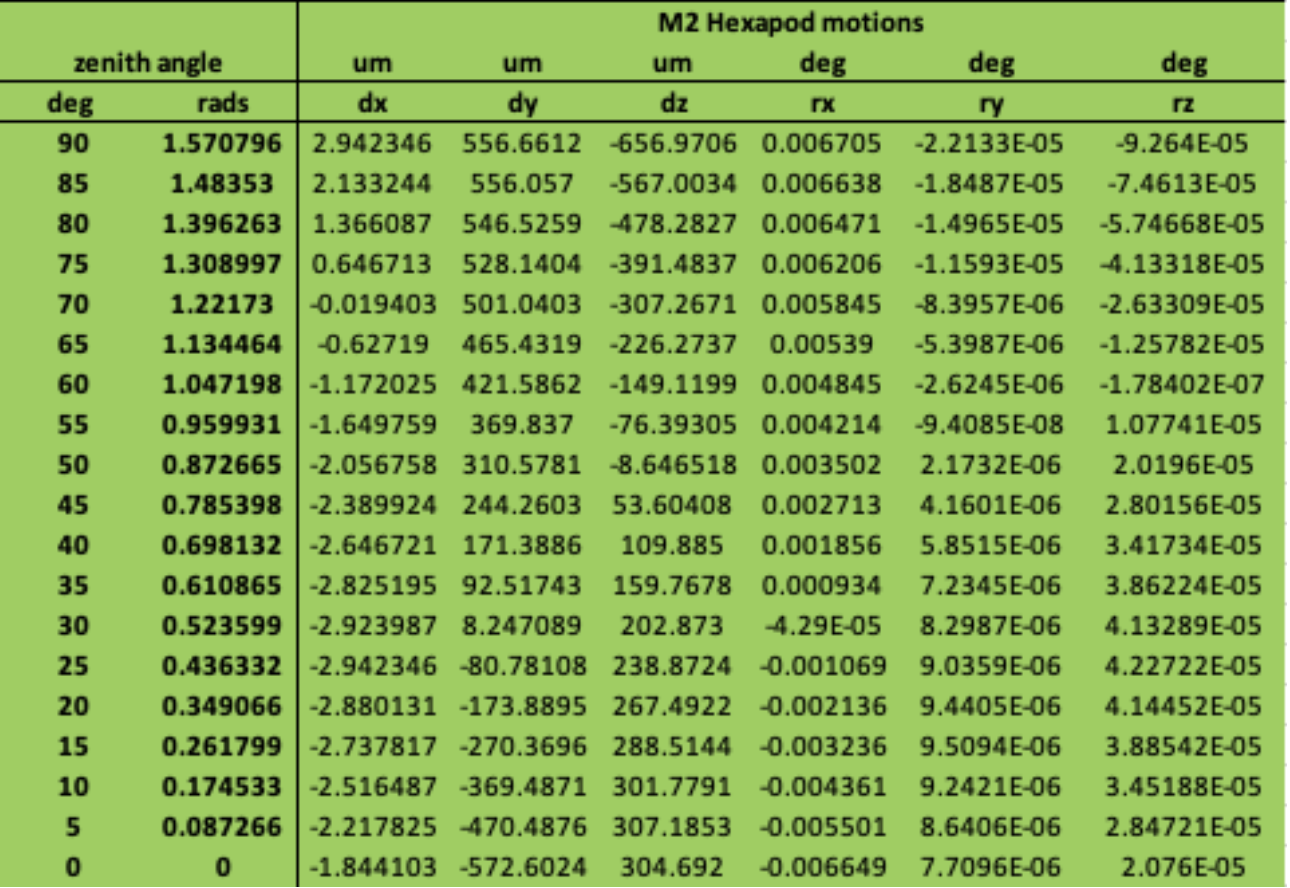
\includegraphics[width=1.5625in,height=\textheight]{jira_imgs/1620.png}\\

}
\hdashrule[0.5ex]{\textwidth}{1pt}{3mm}
  Actual Result \\
{\footnotesize

}
\begin{tabular}{p{2cm}p{14cm}}
\toprule
Step 29 & Step Execution Status: \textbf{ Not Executed } \\ \hline
\end{tabular}
 Description \\
{\footnotesize
In enabled/stationary state, send a move command of (0um, 0um, 800um,
0deg, 0deg, 0deg)

}
\hdashrule[0.5ex]{\textwidth}{1pt}{3mm}
  Expected Result \\
{\footnotesize
The hexapod does not move since it stayed in compensationMode.

}
\hdashrule[0.5ex]{\textwidth}{1pt}{3mm}
  Actual Result \\
{\footnotesize

}
\begin{tabular}{p{2cm}p{14cm}}
\toprule
Step 30 & Step Execution Status: \textbf{ Not Executed } \\ \hline
\end{tabular}
 Description \\
{\footnotesize
Wait 39 seconds.

}
\hdashrule[0.5ex]{\textwidth}{1pt}{3mm}
  Expected Result \\
{\footnotesize

}
\hdashrule[0.5ex]{\textwidth}{1pt}{3mm}
  Actual Result \\
{\footnotesize

}
\begin{tabular}{p{2cm}p{14cm}}
\toprule
Step 31 & Step Execution Status: \textbf{ Not Executed } \\ \hline
\end{tabular}
 Description \\
{\footnotesize
Record the corresponding thermal sensors and verify they are below 19
deg C. If they are above 19 deg C, wait until they are below 19 deg C to
perform the following steps.

}
\hdashrule[0.5ex]{\textwidth}{1pt}{3mm}
  Expected Result \\
{\footnotesize
All actuators are below 19 deg C.

}
\hdashrule[0.5ex]{\textwidth}{1pt}{3mm}
  Actual Result \\
{\footnotesize

}
\begin{tabular}{p{2cm}p{14cm}}
\toprule
Step 32 & Step Execution Status: \textbf{ Not Executed } \\ \hline
\end{tabular}
 Description \\
{\footnotesize
{\textbf{OFFSET TEST}}\\
\textbf{Section 3.1.2 of the attached Software Acceptance Test
Procedure\\
Test Sequence \#4 - Synchronous Offset and Move Commands}\\
In enabled/stationary state, send a move command of (x=500um, y=800um,
z=200um, u=0deg, v=0deg, w=0deg)

}
\hdashrule[0.5ex]{\textwidth}{1pt}{3mm}
  Test Data \\
 {\footnotesize
\textbf{Deviation:} There is no positionSet command anymore. positionSet
and move command replaced by new move command. Now, the hexapod starts
movement directly after receiving the command.\\
\strut \\

}
\hdashrule[0.5ex]{\textwidth}{1pt}{3mm}
  Expected Result \\
{\footnotesize
\begin{itemize}
\tightlist
\item
  The hexapod moves to (x=500um, y=800um, z=200um, u=0deg, v=0deg,
  w=0deg)
\item
  Since the Hexapod is in synchronous mode, the actuators complete the
  move at nearly the same time.
\end{itemize}

}
\hdashrule[0.5ex]{\textwidth}{1pt}{3mm}
  Actual Result \\
{\footnotesize

}
\begin{tabular}{p{2cm}p{14cm}}
\toprule
Step 33 & Step Execution Status: \textbf{ Not Executed } \\ \hline
\end{tabular}
 Description \\
{\footnotesize
In enabled/stationary state, send an offset command of (0um, 0um, 500um,
0deg, 0deg, 0deg).

}
\hdashrule[0.5ex]{\textwidth}{1pt}{3mm}
  Expected Result \\
{\footnotesize
\begin{itemize}
\tightlist
\item
  The hexapod moves only 500um in Z from the previous position
\item
  The actuators complete the move at nearly the same time.
\end{itemize}

}
\hdashrule[0.5ex]{\textwidth}{1pt}{3mm}
  Actual Result \\
{\footnotesize

}
\begin{tabular}{p{2cm}p{14cm}}
\toprule
Step 34 & Step Execution Status: \textbf{ Not Executed } \\ \hline
\end{tabular}
 Description \\
{\footnotesize
Send a move command.~

}
\hdashrule[0.5ex]{\textwidth}{1pt}{3mm}
  Test Data \\
 {\footnotesize
\textbf{Deviation:} Skip this step. The Hexapod has already moved.

}
\hdashrule[0.5ex]{\textwidth}{1pt}{3mm}
  Expected Result \\
{\footnotesize
\begin{itemize}
\tightlist
\item
  The hexapod moves only 500um in Z from the previous position
\item
  The actuators complete the move at nearly the same time.
\end{itemize}

}
\hdashrule[0.5ex]{\textwidth}{1pt}{3mm}
  Actual Result \\
{\footnotesize

}
\begin{tabular}{p{2cm}p{14cm}}
\toprule
Step 35 & Step Execution Status: \textbf{ Not Executed } \\ \hline
\end{tabular}
 Description \\
{\footnotesize
Wait 39s.

}
\hdashrule[0.5ex]{\textwidth}{1pt}{3mm}
  Expected Result \\
{\footnotesize

}
\hdashrule[0.5ex]{\textwidth}{1pt}{3mm}
  Actual Result \\
{\footnotesize

}
\begin{tabular}{p{2cm}p{14cm}}
\toprule
Step 36 & Step Execution Status: \textbf{ Not Executed } \\ \hline
\end{tabular}
 Description \\
{\footnotesize
Record the corresponding DDS events that were generated.

}
\hdashrule[0.5ex]{\textwidth}{1pt}{3mm}
  Expected Result \\
{\footnotesize
\begin{itemize}
\tightlist
\item
  The controllerState.enabledSubstate goes to MOVING\_POINT\_TO\_POINT
  when the move begins and STATIONARY when the move ends
\item
  The inPosition event is True when the move finishes
\item
  The inPosition event is False when the enabledSubstate goes back to
  STATIONARY.
\end{itemize}

}
\hdashrule[0.5ex]{\textwidth}{1pt}{3mm}
  Actual Result \\
{\footnotesize

}
\begin{tabular}{p{2cm}p{14cm}}
\toprule
Step 37 & Step Execution Status: \textbf{ Not Executed } \\ \hline
\end{tabular}
 Description \\
{\footnotesize
\textbf{Section 3.1.2 of the attached Software Acceptance Test
Procedure\\
Test Sequence \#2 -Pivot, PositionSet and Move Commands}\\
In enabled/stationary state, send a move command of
(x=2000um,y=-3500um,z=200um,u=0.01deg,v=-0.05deg, w=0.002deg,sync=true)

}
\hdashrule[0.5ex]{\textwidth}{1pt}{3mm}
  Test Data \\
 {\footnotesize
\textbf{Deviation:} Determine where the original pivot point is before
sending a pivot command of (0, 0, 0).\\
Record any offset commands necessary to test before sending the move
command.

}
\hdashrule[0.5ex]{\textwidth}{1pt}{3mm}
  Expected Result \\
{\footnotesize
The hexapod moves to the commanded position

}
\hdashrule[0.5ex]{\textwidth}{1pt}{3mm}
  Actual Result \\
{\footnotesize

}
\begin{tabular}{p{2cm}p{14cm}}
\toprule
Step 38 & Step Execution Status: \textbf{ Not Executed } \\ \hline
\end{tabular}
 Description \\
{\footnotesize
In the enabled/stationary state, send a pivot command of (0,0,0).

}
\hdashrule[0.5ex]{\textwidth}{1pt}{3mm}
  Expected Result \\
{\footnotesize
The actuator positions do not change but the hexapod position changes to
account for the new pivot point.

}
\hdashrule[0.5ex]{\textwidth}{1pt}{3mm}
  Actual Result \\
{\footnotesize

}
\begin{tabular}{p{2cm}p{14cm}}
\toprule
Step 39 & Step Execution Status: \textbf{ Not Executed } \\ \hline
\end{tabular}
 Description \\
{\footnotesize
In the enabled/stationary state, send again the move command of
(x=2000um, y=-3500um, z=200um, u=0.01deg, v=-0.05deg,
w=0.002deg,sync=true)

}
\hdashrule[0.5ex]{\textwidth}{1pt}{3mm}
  Test Data \\
 {\footnotesize
\textbf{Deviation:} Record any offset commands necessary to test before
sending the move command.\\
\strut \\

}
\hdashrule[0.5ex]{\textwidth}{1pt}{3mm}
  Expected Result \\
{\footnotesize
Confirm the hexapod moves to the commanded position and the actuators
change position to account for the new pivot point. Position values in
the EFD appear different.

}
\hdashrule[0.5ex]{\textwidth}{1pt}{3mm}
  Actual Result \\
{\footnotesize

}
\begin{tabular}{p{2cm}p{14cm}}
\toprule
Step 40 & Step Execution Status: \textbf{ Not Executed } \\ \hline
\end{tabular}
 Description \\
{\footnotesize
Wait 39s.

}
\hdashrule[0.5ex]{\textwidth}{1pt}{3mm}
  Expected Result \\
{\footnotesize

}
\hdashrule[0.5ex]{\textwidth}{1pt}{3mm}
  Actual Result \\
{\footnotesize

}
\begin{tabular}{p{2cm}p{14cm}}
\toprule
Step 41 & Step Execution Status: \textbf{ Not Executed } \\ \hline
\end{tabular}
 Description \\
{\footnotesize
\textbf{{CONFIGURE LIMITS TEST}}\\
\textbf{Section 3.1.2 of the attached Software Acceptance Test
Procedure\\
Test Sequence \#6 - configureLimits Command}\\
In enabled/stationary state, send a configureLimits command of (12000um,
-1000um, 1000um, 0.1, -0.1, 0.05)

}
\hdashrule[0.5ex]{\textwidth}{1pt}{3mm}
  Test Data \\
 {\footnotesize
\textbf{Deviation:} Skip complete test. This test uses an obsolete
command. The configuration is now done before and should not be changed
this state

}
\hdashrule[0.5ex]{\textwidth}{1pt}{3mm}
  Expected Result \\
{\footnotesize
The command is rejected for being outside acceptable limits.

}
\hdashrule[0.5ex]{\textwidth}{1pt}{3mm}
  Actual Result \\
{\footnotesize

}
\begin{tabular}{p{2cm}p{14cm}}
\toprule
Step 42 & Step Execution Status: \textbf{ Not Executed } \\ \hline
\end{tabular}
 Description \\
{\footnotesize
In enabled/stationary state, send a configureLimits command of (1000um,
-1000um, 1000um, 0.1, -0.1, 0.05)

}
\hdashrule[0.5ex]{\textwidth}{1pt}{3mm}
  Expected Result \\
{\footnotesize
The command is accepted.

}
\hdashrule[0.5ex]{\textwidth}{1pt}{3mm}
  Actual Result \\
{\footnotesize

}
\begin{tabular}{p{2cm}p{14cm}}
\toprule
Step 43 & Step Execution Status: \textbf{ Not Executed } \\ \hline
\end{tabular}
 Description \\
{\footnotesize
In enabled/stationary state, send a positionSet command of (1200um, 0um,
200um, 0deg, 0deg, 0deg)

}
\hdashrule[0.5ex]{\textwidth}{1pt}{3mm}
  Expected Result \\
{\footnotesize
The command is rejected for being outside of range limits

}
\hdashrule[0.5ex]{\textwidth}{1pt}{3mm}
  Actual Result \\
{\footnotesize

}
\begin{tabular}{p{2cm}p{14cm}}
\toprule
Step 44 & Step Execution Status: \textbf{ Not Executed } \\ \hline
\end{tabular}
 Description \\
{\footnotesize
In enabled/stationary state, send a positionSet command of (990um,
990um, 200um, 0deg, 0deg, 0deg)

}
\hdashrule[0.5ex]{\textwidth}{1pt}{3mm}
  Expected Result \\
{\footnotesize
The command is rejected for being outside of range limits.

}
\hdashrule[0.5ex]{\textwidth}{1pt}{3mm}
  Actual Result \\
{\footnotesize

}
\begin{tabular}{p{2cm}p{14cm}}
\toprule
Step 45 & Step Execution Status: \textbf{ Not Executed } \\ \hline
\end{tabular}
 Description \\
{\footnotesize
In enabled/stationary state, send a positionSet command of (500um,
500um, 200um, 0deg, 0.1 deg, 0.01deg)

}
\hdashrule[0.5ex]{\textwidth}{1pt}{3mm}
  Expected Result \\
{\footnotesize
The command is accepted.

}
\hdashrule[0.5ex]{\textwidth}{1pt}{3mm}
  Actual Result \\
{\footnotesize

}
\begin{tabular}{p{2cm}p{14cm}}
\toprule
Step 46 & Step Execution Status: \textbf{ Not Executed } \\ \hline
\end{tabular}
 Description \\
{\footnotesize
Send a move command.

}
\hdashrule[0.5ex]{\textwidth}{1pt}{3mm}
  Expected Result \\
{\footnotesize
The previously accepted command is executed.

}
\hdashrule[0.5ex]{\textwidth}{1pt}{3mm}
  Actual Result \\
{\footnotesize

}
\begin{tabular}{p{2cm}p{14cm}}
\toprule
Step 47 & Step Execution Status: \textbf{ Not Executed } \\ \hline
\end{tabular}
 Description \\
{\footnotesize
Record the DDS events that were generated.

}
\hdashrule[0.5ex]{\textwidth}{1pt}{3mm}
  Expected Result \\
{\footnotesize
The change is reflected in the settingsApplied event and the EUI.

}
\hdashrule[0.5ex]{\textwidth}{1pt}{3mm}
  Actual Result \\
{\footnotesize

}
\begin{tabular}{p{2cm}p{14cm}}
\toprule
Step 48 & Step Execution Status: \textbf{ Not Executed } \\ \hline
\end{tabular}
 Description \\
{\footnotesize
{\textbf{CONFIGURE ACCELERATION TEST}}\\
\textbf{Section 3.1.2 of the attached Software Acceptance Test
Procedure\\
Test Sequence \#7 - configureAcceleration Command}\\
In enabled/stationary state, at a position of (0, 0, 0, 0, 0, 0) with
the velocity and acceleration values set to their nominal values, send a
positionSet command of (0um, 0um, 4900um, 0 deg, 0 deg, 0 deg, s).

}
\hdashrule[0.5ex]{\textwidth}{1pt}{3mm}
  Test Data \\
 {\footnotesize
\textbf{Deviation:} Skip complete test. This test uses an obsolete
command. The configuration is now done before and should not be changed
this state

}
\hdashrule[0.5ex]{\textwidth}{1pt}{3mm}
  Expected Result \\
{\footnotesize
The hexapod doesn\textquotesingle t move.

}
\hdashrule[0.5ex]{\textwidth}{1pt}{3mm}
  Actual Result \\
{\footnotesize

}
\begin{tabular}{p{2cm}p{14cm}}
\toprule
Step 49 & Step Execution Status: \textbf{ Not Executed } \\ \hline
\end{tabular}
 Description \\
{\footnotesize
Send a move command.

}
\hdashrule[0.5ex]{\textwidth}{1pt}{3mm}
  Expected Result \\
{\footnotesize
The move takes approximately 9 seconds to complete.

}
\hdashrule[0.5ex]{\textwidth}{1pt}{3mm}
  Actual Result \\
{\footnotesize

}
\begin{tabular}{p{2cm}p{14cm}}
\toprule
Step 50 & Step Execution Status: \textbf{ Not Executed } \\ \hline
\end{tabular}
 Description \\
{\footnotesize
Send a configureAcceleration command of 1000.

}
\hdashrule[0.5ex]{\textwidth}{1pt}{3mm}
  Expected Result \\
{\footnotesize
~Confirm command is rejected for being outside of acceptable limits.

}
\hdashrule[0.5ex]{\textwidth}{1pt}{3mm}
  Actual Result \\
{\footnotesize

}
\begin{tabular}{p{2cm}p{14cm}}
\toprule
Step 51 & Step Execution Status: \textbf{ Not Executed } \\ \hline
\end{tabular}
 Description \\
{\footnotesize
Send a configureAcceleration command of 100.

}
\hdashrule[0.5ex]{\textwidth}{1pt}{3mm}
  Expected Result \\
{\footnotesize
The command is accepted.~

}
\hdashrule[0.5ex]{\textwidth}{1pt}{3mm}
  Actual Result \\
{\footnotesize

}
\begin{tabular}{p{2cm}p{14cm}}
\toprule
Step 52 & Step Execution Status: \textbf{ Not Executed } \\ \hline
\end{tabular}
 Description \\
{\footnotesize
In enabled/stationary state, send a postionSet command of (0um, 0um,
0um, 0 deg, 0 deg, 0 deg, s).

}
\hdashrule[0.5ex]{\textwidth}{1pt}{3mm}
  Expected Result \\
{\footnotesize
The hexapod doesn\textquotesingle t move.

}
\hdashrule[0.5ex]{\textwidth}{1pt}{3mm}
  Actual Result \\
{\footnotesize

}
\begin{tabular}{p{2cm}p{14cm}}
\toprule
Step 53 & Step Execution Status: \textbf{ Not Executed } \\ \hline
\end{tabular}
 Description \\
{\footnotesize
Send a move command.~

}
\hdashrule[0.5ex]{\textwidth}{1pt}{3mm}
  Expected Result \\
{\footnotesize
It takes approximately 13 seconds to complete the commanded move with
the reduced acceleration value.

}
\hdashrule[0.5ex]{\textwidth}{1pt}{3mm}
  Actual Result \\
{\footnotesize

}
\begin{tabular}{p{2cm}p{14cm}}
\toprule
Step 54 & Step Execution Status: \textbf{ Not Executed } \\ \hline
\end{tabular}
 Description \\
{\footnotesize
Send a configureAcceleration command of 500 to return the acceleration
limit to its nominal value.

}
\hdashrule[0.5ex]{\textwidth}{1pt}{3mm}
  Expected Result \\
{\footnotesize
The command is accepted.

}
\hdashrule[0.5ex]{\textwidth}{1pt}{3mm}
  Actual Result \\
{\footnotesize

}
\begin{tabular}{p{2cm}p{14cm}}
\toprule
Step 55 & Step Execution Status: \textbf{ Not Executed } \\ \hline
\end{tabular}
 Description \\
{\footnotesize
Record the corresponding DDS events that were generated.

}
\hdashrule[0.5ex]{\textwidth}{1pt}{3mm}
  Expected Result \\
{\footnotesize
The change is reflected in the settingsApplied event and the EUI.

}
\hdashrule[0.5ex]{\textwidth}{1pt}{3mm}
  Actual Result \\
{\footnotesize

}
\begin{tabular}{p{2cm}p{14cm}}
\toprule
Step 56 & Step Execution Status: \textbf{ Not Executed } \\ \hline
\end{tabular}
 Description \\
{\footnotesize
\textbf{{CONFIGURE VELOCITY TEST}}\\
\textbf{Section 3.1.2 of the attached Software Acceptance Test
Procedure\\
Test Sequence \#8 - configureVelocity Command}\\
In enabled/stationary state, at a position of (0, 0, 0, 0, 0, 0), send a
configureVelocity command of (10000, .01, 100, .01).

}
\hdashrule[0.5ex]{\textwidth}{1pt}{3mm}
  Test Data \\
 {\footnotesize
\textbf{Deviation:} Skip complete test. This test uses an obsolete
command. The configuration is now done before and should not be changed
this state

}
\hdashrule[0.5ex]{\textwidth}{1pt}{3mm}
  Expected Result \\
{\footnotesize
This command is rejected for being outside of acceptable limits.

}
\hdashrule[0.5ex]{\textwidth}{1pt}{3mm}
  Actual Result \\
{\footnotesize

}
\begin{tabular}{p{2cm}p{14cm}}
\toprule
Step 57 & Step Execution Status: \textbf{ Not Executed } \\ \hline
\end{tabular}
 Description \\
{\footnotesize
In enabled/stationary state, send a configureVelocity command of (100,
.01, 200, .01).~

}
\hdashrule[0.5ex]{\textwidth}{1pt}{3mm}
  Expected Result \\
{\footnotesize
This command is accepted.

}
\hdashrule[0.5ex]{\textwidth}{1pt}{3mm}
  Actual Result \\
{\footnotesize

}
\begin{tabular}{p{2cm}p{14cm}}
\toprule
Step 58 & Step Execution Status: \textbf{ Not Executed } \\ \hline
\end{tabular}
 Description \\
{\footnotesize
In enabled/stationary state, send a positionSet command of (0, 0um,
2000um, 0 deg, 0 deg, 0 deg, s).

}
\hdashrule[0.5ex]{\textwidth}{1pt}{3mm}
  Expected Result \\
{\footnotesize
The command is accepted

}
\hdashrule[0.5ex]{\textwidth}{1pt}{3mm}
  Actual Result \\
{\footnotesize

}
\begin{tabular}{p{2cm}p{14cm}}
\toprule
Step 59 & Step Execution Status: \textbf{ Not Executed } \\ \hline
\end{tabular}
 Description \\
{\footnotesize
Send a move command.~

}
\hdashrule[0.5ex]{\textwidth}{1pt}{3mm}
  Expected Result \\
{\footnotesize
It takes approximately 20 seconds to complete the commanded move.

}
\hdashrule[0.5ex]{\textwidth}{1pt}{3mm}
  Actual Result \\
{\footnotesize

}
\begin{tabular}{p{2cm}p{14cm}}
\toprule
Step 60 & Step Execution Status: \textbf{ Not Executed } \\ \hline
\end{tabular}
 Description \\
{\footnotesize
In enabled/stationary state, send a configureVelocity command of (100,
.01, 100, .01).~

}
\hdashrule[0.5ex]{\textwidth}{1pt}{3mm}
  Expected Result \\
{\footnotesize
This command is accepted.

}
\hdashrule[0.5ex]{\textwidth}{1pt}{3mm}
  Actual Result \\
{\footnotesize

}
\begin{tabular}{p{2cm}p{14cm}}
\toprule
Step 61 & Step Execution Status: \textbf{ Not Executed } \\ \hline
\end{tabular}
 Description \\
{\footnotesize
In enabled/stationary state, send an offset command of (0, 0um, 2000um,
0 deg, 0 deg, 0 deg).

}
\hdashrule[0.5ex]{\textwidth}{1pt}{3mm}
  Expected Result \\
{\footnotesize
This command is accepted

}
\hdashrule[0.5ex]{\textwidth}{1pt}{3mm}
  Actual Result \\
{\footnotesize

}
\begin{tabular}{p{2cm}p{14cm}}
\toprule
Step 62 & Step Execution Status: \textbf{ Not Executed } \\ \hline
\end{tabular}
 Description \\
{\footnotesize
Send a move command.~

}
\hdashrule[0.5ex]{\textwidth}{1pt}{3mm}
  Expected Result \\
{\footnotesize
It takes approximately 40 seconds to complete the commanded move.

}
\hdashrule[0.5ex]{\textwidth}{1pt}{3mm}
  Actual Result \\
{\footnotesize

}
\begin{tabular}{p{2cm}p{14cm}}
\toprule
Step 63 & Step Execution Status: \textbf{ Not Executed } \\ \hline
\end{tabular}
 Description \\
{\footnotesize
Record the corresponding DDS events that were generated:

}
\hdashrule[0.5ex]{\textwidth}{1pt}{3mm}
  Expected Result \\
{\footnotesize
The change is reflected in the settingsApplied event and the EUI.

}
\hdashrule[0.5ex]{\textwidth}{1pt}{3mm}
  Actual Result \\
{\footnotesize

}
\begin{tabular}{p{2cm}p{14cm}}
\toprule
Step 64 & Step Execution Status: \textbf{ Not Executed } \\ \hline
\end{tabular}
 Description \\
{\footnotesize
\textbf{Section 3.3.2 of the attached Software Acceptance Test Procedure
Hexapod Action on State Commands}\\
In the Offline/PublishOnly state, send all commands

}
\hdashrule[0.5ex]{\textwidth}{1pt}{3mm}
  Expected Result \\
{\footnotesize
There is no change and command is rejected.

}
\hdashrule[0.5ex]{\textwidth}{1pt}{3mm}
  Actual Result \\
{\footnotesize

}
\begin{tabular}{p{2cm}p{14cm}}
\toprule
Step 65 & Step Execution Status: \textbf{ Not Executed } \\ \hline
\end{tabular}
 Description \\
{\footnotesize
In the Offline/Available state, send an enterControl command

}
\hdashrule[0.5ex]{\textwidth}{1pt}{3mm}
  Expected Result \\
{\footnotesize
The system enters the Standby state.

}
\hdashrule[0.5ex]{\textwidth}{1pt}{3mm}
  Actual Result \\
{\footnotesize

}
\begin{tabular}{p{2cm}p{14cm}}
\toprule
Step 66 & Step Execution Status: \textbf{ Not Executed } \\ \hline
\end{tabular}
 Description \\
{\footnotesize
In the Standby state, send any command except start or exitControl

}
\hdashrule[0.5ex]{\textwidth}{1pt}{3mm}
  Expected Result \\
{\footnotesize
There is no change and command is rejected.

}
\hdashrule[0.5ex]{\textwidth}{1pt}{3mm}
  Actual Result \\
{\footnotesize

}
\begin{tabular}{p{2cm}p{14cm}}
\toprule
Step 67 & Step Execution Status: \textbf{ Not Executed } \\ \hline
\end{tabular}
 Description \\
{\footnotesize
In the Standby state, send an exitControl command.

}
\hdashrule[0.5ex]{\textwidth}{1pt}{3mm}
  Expected Result \\
{\footnotesize
The system transitions into the Offline/Available state.

}
\hdashrule[0.5ex]{\textwidth}{1pt}{3mm}
  Actual Result \\
{\footnotesize

}
\begin{tabular}{p{2cm}p{14cm}}
\toprule
Step 68 & Step Execution Status: \textbf{ Not Executed } \\ \hline
\end{tabular}
 Description \\
{\footnotesize
In the Standby state, send a start command.

}
\hdashrule[0.5ex]{\textwidth}{1pt}{3mm}
  Expected Result \\
{\footnotesize
The system transitions into the Disabled state.

}
\hdashrule[0.5ex]{\textwidth}{1pt}{3mm}
  Actual Result \\
{\footnotesize

}
\begin{tabular}{p{2cm}p{14cm}}
\toprule
Step 69 & Step Execution Status: \textbf{ Not Executed } \\ \hline
\end{tabular}
 Description \\
{\footnotesize
In the Disabled state, send any command except for the enabled or
standby command.

}
\hdashrule[0.5ex]{\textwidth}{1pt}{3mm}
  Expected Result \\
{\footnotesize
There is no change and the command is rejected.

}
\hdashrule[0.5ex]{\textwidth}{1pt}{3mm}
  Actual Result \\
{\footnotesize

}
\begin{tabular}{p{2cm}p{14cm}}
\toprule
Step 70 & Step Execution Status: \textbf{ Not Executed } \\ \hline
\end{tabular}
 Description \\
{\footnotesize
In the Disabled state, send the standby command.

}
\hdashrule[0.5ex]{\textwidth}{1pt}{3mm}
  Expected Result \\
{\footnotesize
The system transitions into the Standby state.

}
\hdashrule[0.5ex]{\textwidth}{1pt}{3mm}
  Actual Result \\
{\footnotesize

}
\begin{tabular}{p{2cm}p{14cm}}
\toprule
Step 71 & Step Execution Status: \textbf{ Not Executed } \\ \hline
\end{tabular}
 Description \\
{\footnotesize
In the Disabled state, send the enable command.

}
\hdashrule[0.5ex]{\textwidth}{1pt}{3mm}
  Expected Result \\
{\footnotesize
The system transitions into the Enabled/Stationary state.

}
\hdashrule[0.5ex]{\textwidth}{1pt}{3mm}
  Actual Result \\
{\footnotesize

}
\begin{tabular}{p{2cm}p{14cm}}
\toprule
Step 72 & Step Execution Status: \textbf{ Not Executed } \\ \hline
\end{tabular}
 Description \\
{\footnotesize
In the Enabled/Stationary state, send either the enterControl command,
exitControl command, start command, clearError command, or enable
command.

}
\hdashrule[0.5ex]{\textwidth}{1pt}{3mm}
  Expected Result \\
{\footnotesize
There is no change and command is rejected.

}
\hdashrule[0.5ex]{\textwidth}{1pt}{3mm}
  Actual Result \\
{\footnotesize

}
\begin{tabular}{p{2cm}p{14cm}}
\toprule
Step 73 & Step Execution Status: \textbf{ Not Executed } \\ \hline
\end{tabular}
 Description \\
{\footnotesize
In the Enabled/Stationary state, send a disable command.

}
\hdashrule[0.5ex]{\textwidth}{1pt}{3mm}
  Expected Result \\
{\footnotesize
The system transitions into Disabled state.

}
\hdashrule[0.5ex]{\textwidth}{1pt}{3mm}
  Actual Result \\
{\footnotesize

}
\begin{tabular}{p{2cm}p{14cm}}
\toprule
Step 74 & Step Execution Status: \textbf{ Not Executed } \\ \hline
\end{tabular}
 Description \\
{\footnotesize
In the Fault state, send any command except the clearError command.

}
\hdashrule[0.5ex]{\textwidth}{1pt}{3mm}
  Expected Result \\
{\footnotesize
There is no change and command is rejected.

}
\hdashrule[0.5ex]{\textwidth}{1pt}{3mm}
  Actual Result \\
{\footnotesize

}
\begin{tabular}{p{2cm}p{14cm}}
\toprule
Step 75 & Step Execution Status: \textbf{ Not Executed } \\ \hline
\end{tabular}
 Description \\
{\footnotesize
In the Fault state, send the clearError command.

}
\hdashrule[0.5ex]{\textwidth}{1pt}{3mm}
  Expected Result \\
{\footnotesize
The system transitions into the Offline/PublishOnly state.

}
\hdashrule[0.5ex]{\textwidth}{1pt}{3mm}
  Actual Result \\
{\footnotesize

}
\begin{tabular}{p{2cm}p{14cm}}
\toprule
Step 76 & Step Execution Status: \textbf{ Not Executed } \\ \hline
\end{tabular}
 Description \\
{\footnotesize
\textbf{Section 4 of the attached Software Acceptance Test Procedure}\\
In the Enabled/Stationary state, unplug a motor encoder cable for one of
the actuators.\textbf{}\\

}
\hdashrule[0.5ex]{\textwidth}{1pt}{3mm}
  Expected Result \\
{\footnotesize
A Drive Fault error event is created and the system transitions to Fault
state.

}
\hdashrule[0.5ex]{\textwidth}{1pt}{3mm}
  Actual Result \\
{\footnotesize

}
\begin{tabular}{p{2cm}p{14cm}}
\toprule
Step 77 & Step Execution Status: \textbf{ Not Executed } \\ \hline
\end{tabular}
 Description \\
{\footnotesize
In the Enabled/Stationary state, unplug a linear encoder cable for one
of the actuators.

}
\hdashrule[0.5ex]{\textwidth}{1pt}{3mm}
  Expected Result \\
{\footnotesize
A Drive Fault error event is created and the system transitions to Fault
state.

}
\hdashrule[0.5ex]{\textwidth}{1pt}{3mm}
  Actual Result \\
{\footnotesize

}
\begin{tabular}{p{2cm}p{14cm}}
\toprule
Step 78 & Step Execution Status: \textbf{ Not Executed } \\ \hline
\end{tabular}
 Description \\
{\footnotesize
Unplug a motor power cable from one of the actuators and command a Move.

}
\hdashrule[0.5ex]{\textwidth}{1pt}{3mm}
  Expected Result \\
{\footnotesize
A Following Error event is created and the system transitions to Fault
state.

}
\hdashrule[0.5ex]{\textwidth}{1pt}{3mm}
  Actual Result \\
{\footnotesize

}
\begin{tabular}{p{2cm}p{14cm}}
\toprule
Step 79 & Step Execution Status: \textbf{ Not Executed } \\ \hline
\end{tabular}
 Description \\
{\footnotesize
Activate an extension limit switch on one of the actuators by removing
the limit switch cover and manually tripping.

}
\hdashrule[0.5ex]{\textwidth}{1pt}{3mm}
  Expected Result \\
{\footnotesize
An Extended Limit Switch error event is created and the system
transitions into Fault state.

}
\hdashrule[0.5ex]{\textwidth}{1pt}{3mm}
  Actual Result \\
{\footnotesize

}
\begin{tabular}{p{2cm}p{14cm}}
\toprule
Step 80 & Step Execution Status: \textbf{ Not Executed } \\ \hline
\end{tabular}
 Description \\
{\footnotesize
Activate a retraction limit switch on one of the actuators by removing
the limit switch cover and manually tripping.

}
\hdashrule[0.5ex]{\textwidth}{1pt}{3mm}
  Expected Result \\
{\footnotesize
A Retracted Limit Switch error event is created and the system
transitions into Fault state.

}
\hdashrule[0.5ex]{\textwidth}{1pt}{3mm}
  Actual Result \\
{\footnotesize

}
\begin{tabular}{p{2cm}p{14cm}}
\toprule
Step 81 & Step Execution Status: \textbf{ Not Executed } \\ \hline
\end{tabular}
 Description \\
{\footnotesize
Unplug the Ethercat cable between the control PC and the first Copley
XE2 drive.

}
\hdashrule[0.5ex]{\textwidth}{1pt}{3mm}
  Expected Result \\
{\footnotesize
An Ethercat Lost event is created and the system transitions to Fault
state.

}
\hdashrule[0.5ex]{\textwidth}{1pt}{3mm}
  Actual Result \\
{\footnotesize

}



\newpage
\appendix
%Make sure lsst-texmf/bin/generateAcronyms.py is in your path
\section{Acronyms used in this document}\label{sec:acronyms}
\addtocounter{table}{-1}
\begin{longtable}{p{0.145\textwidth}p{0.8\textwidth}}\hline
\textbf{Acronym} & \textbf{Description}  \\\hline

EFD & Engineering and Facility Database \\\hline
GUI & Graphical User Interface \\\hline
LSST & Large Synoptic Survey Telescope \\\hline
LUT & Look-Up Table \\\hline
PMCS & Project Management Controls System \\\hline
Source & A single detection of an astrophysical object in an image, the characteristics for which are stored in the Source Catalog of the DRP database. The association of Sources that are non-moving lead to Objects; the association of moving Sources leads to Solar System Objects. (Note that in non-LSST usage "source" is often used for what LSST calls an Object.) \\\hline
\end{longtable}


\end{document}
